%int-01
\begin{figure}[ht]
  \centering
  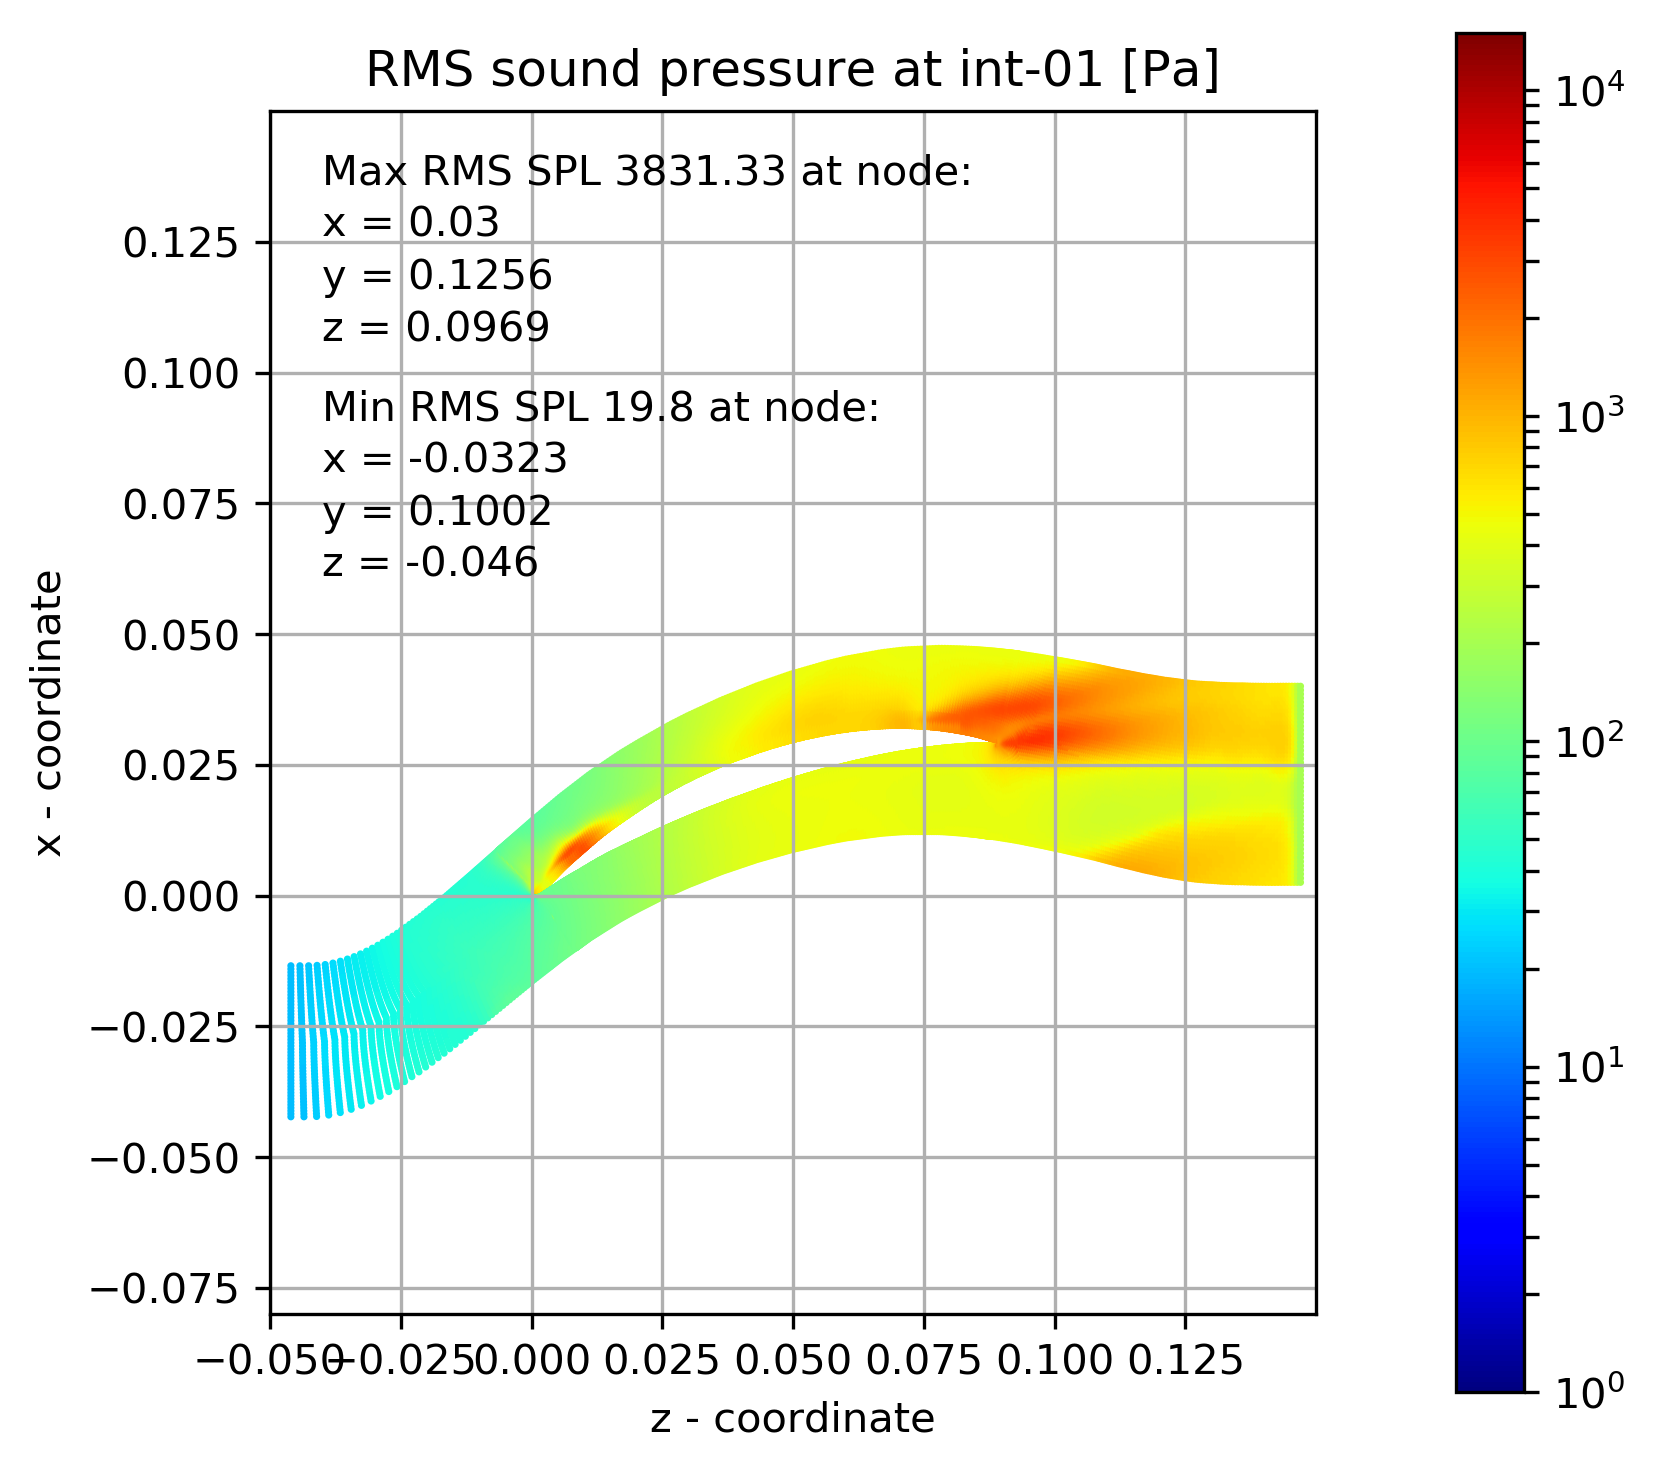
\includegraphics[width=0.75\textwidth]{Figures/int-01-rms-spl.png} \label{int-01-rms-spl}
  \caption{RMS Sound pressure at int-01 mark}
  
  \vspace*{\floatsep}% https://tex.stackexchange.com/q/26521/5764

  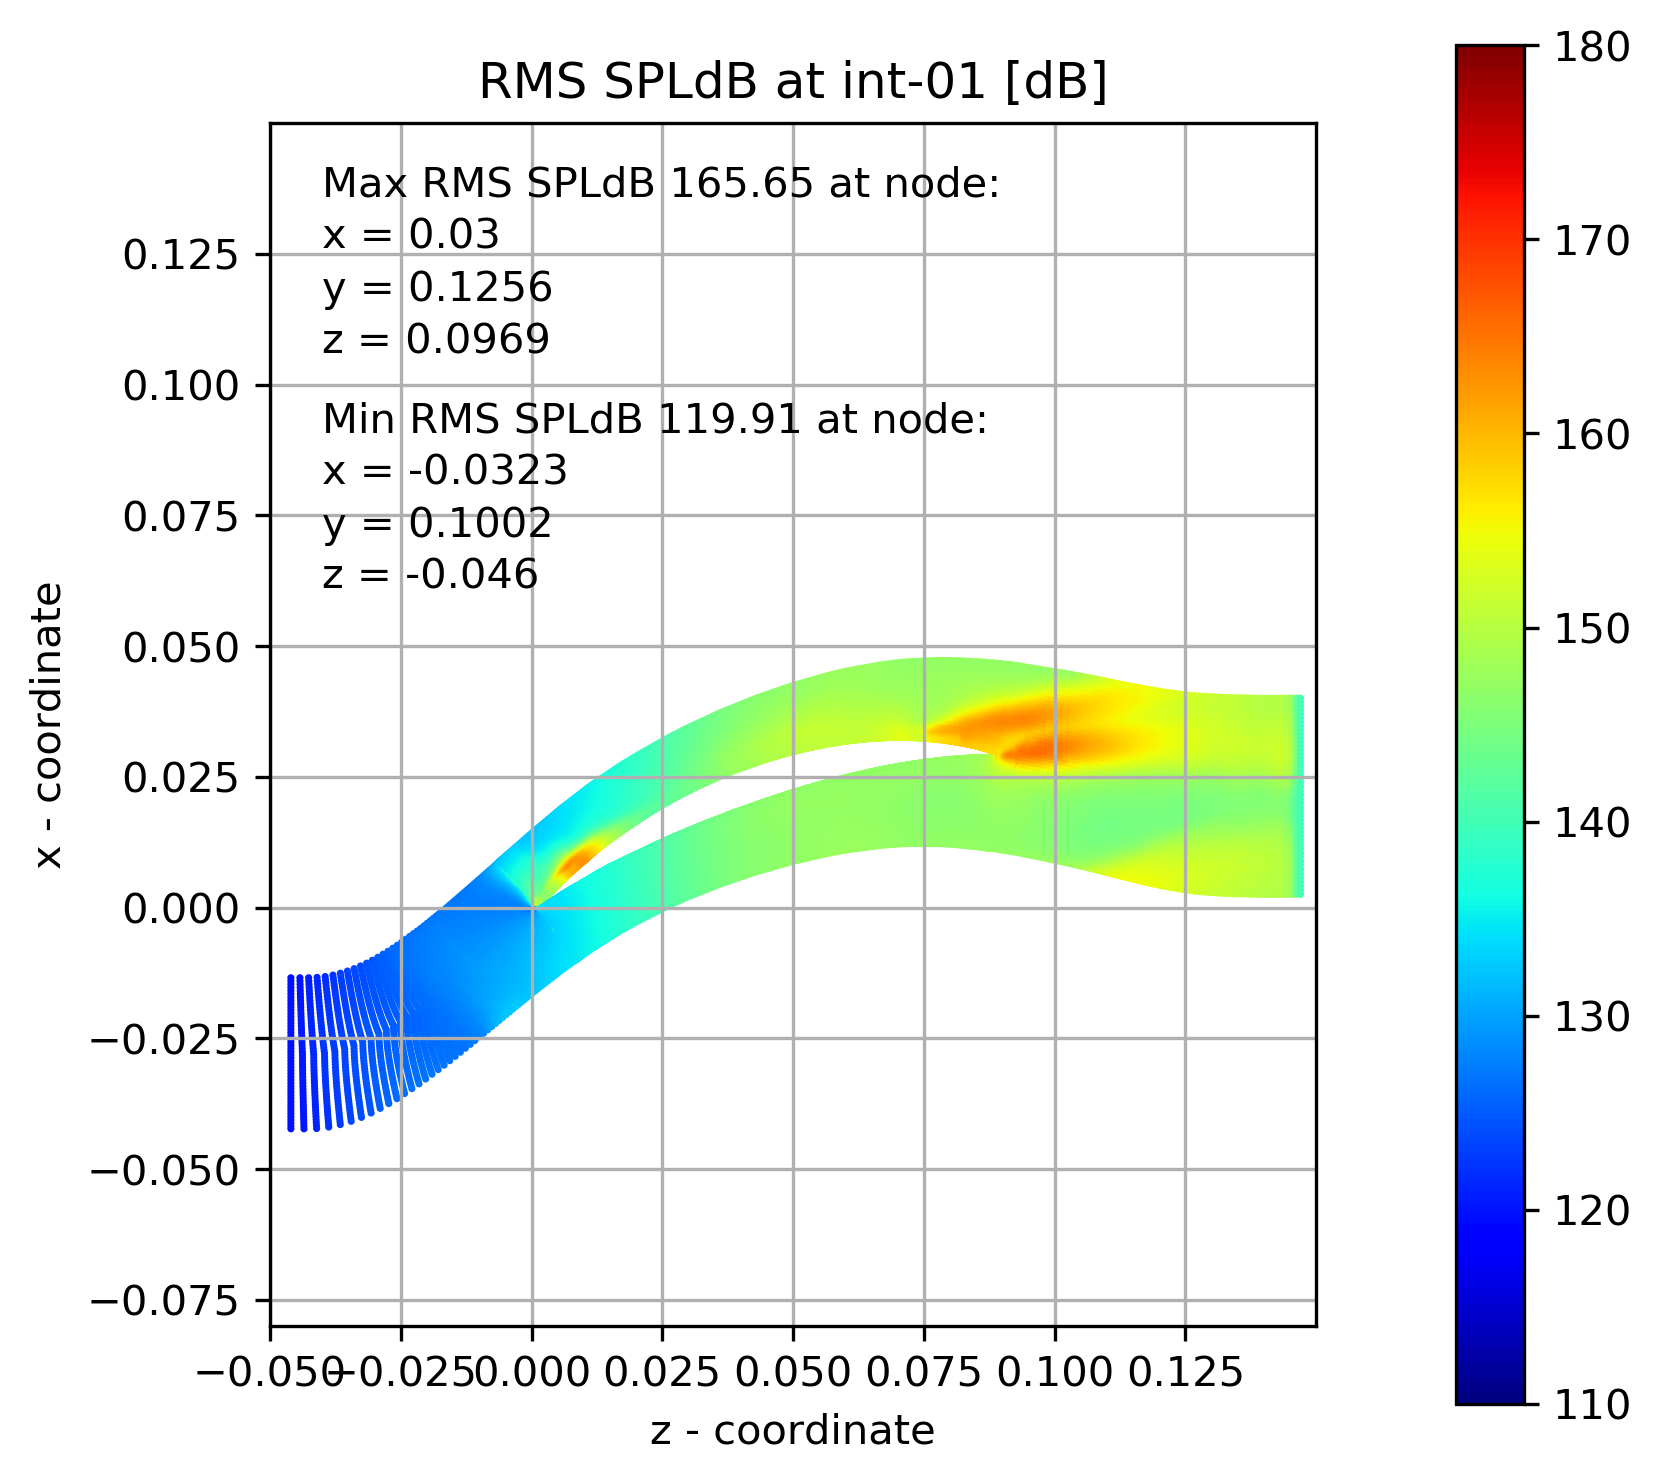
\includegraphics[width=0.75\textwidth]{Figures/int-01-rms-spldb.png} \label{int-01-rms-spldb}
  \caption{RMS Sound pressure decibel level at int-01 mark}
\end{figure}
%int-01
\begin{figure}[ht]
  \centering
  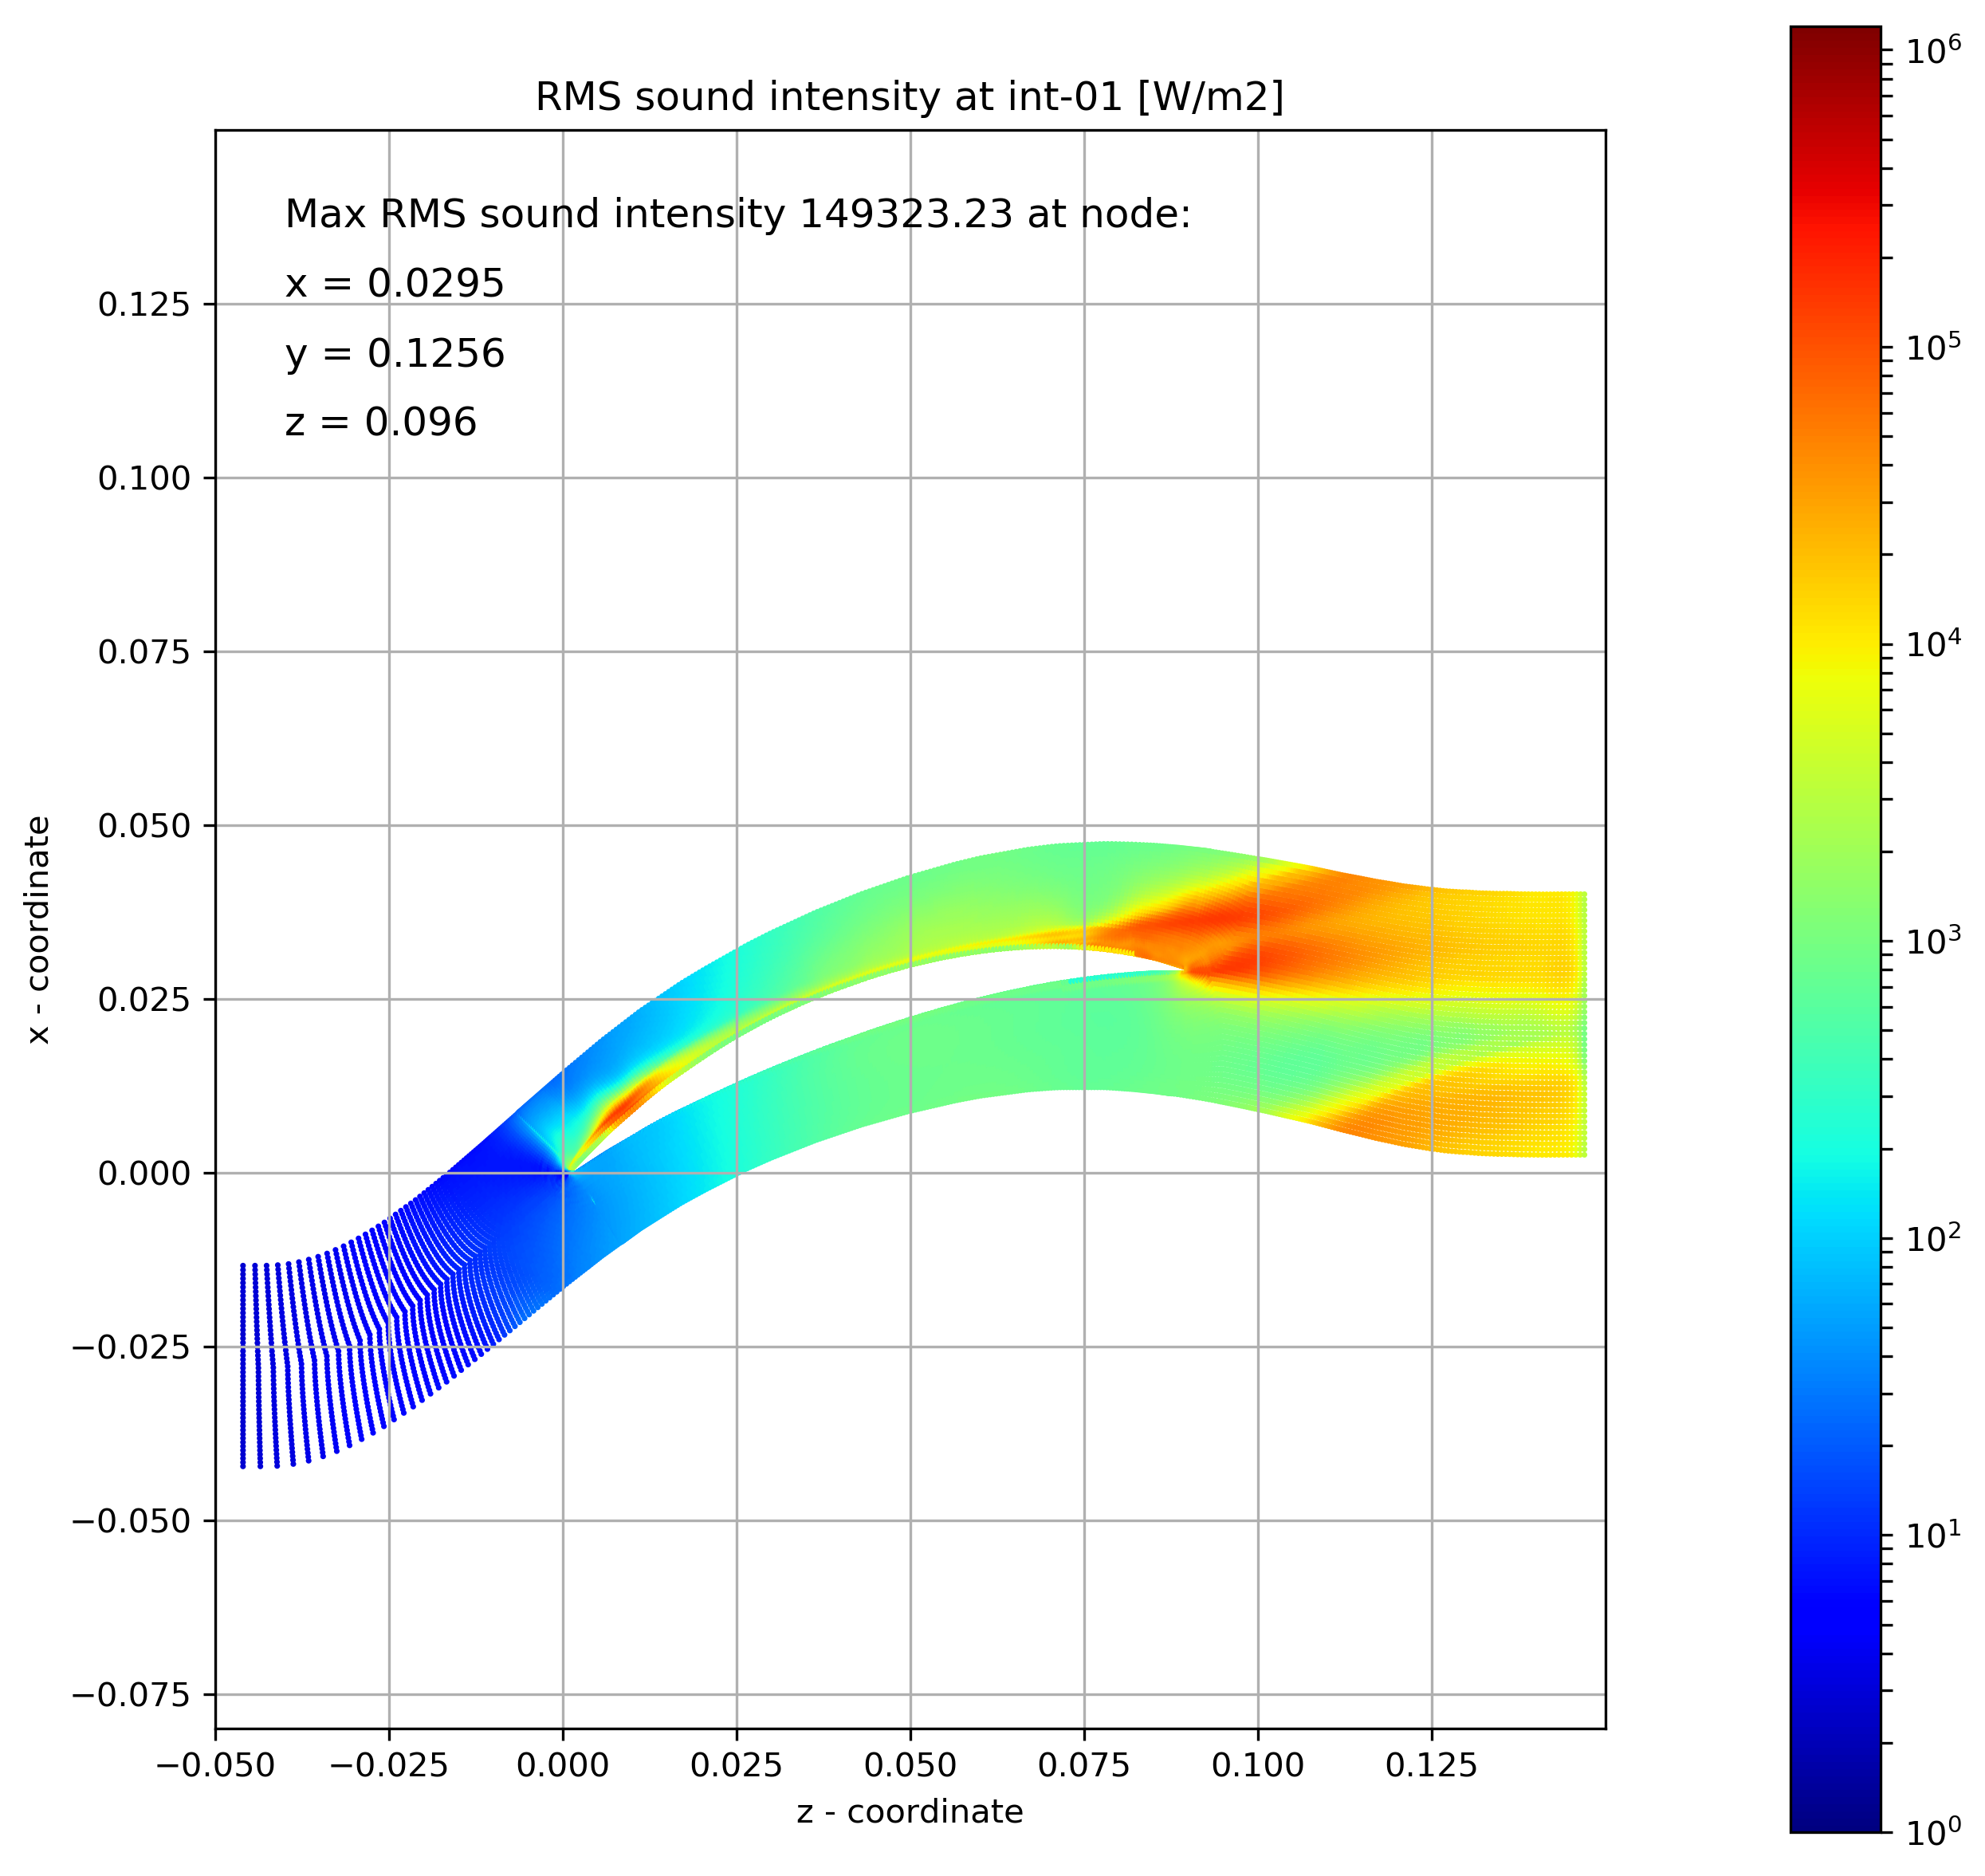
\includegraphics[width=0.75\textwidth]{Figures/int-01-rms-sil.png} \label{int-01-rms-sil}
  \caption{RMS Sound intensity at int-01 mark}
  
  \vspace*{\floatsep}% https://tex.stackexchange.com/q/26521/5764

  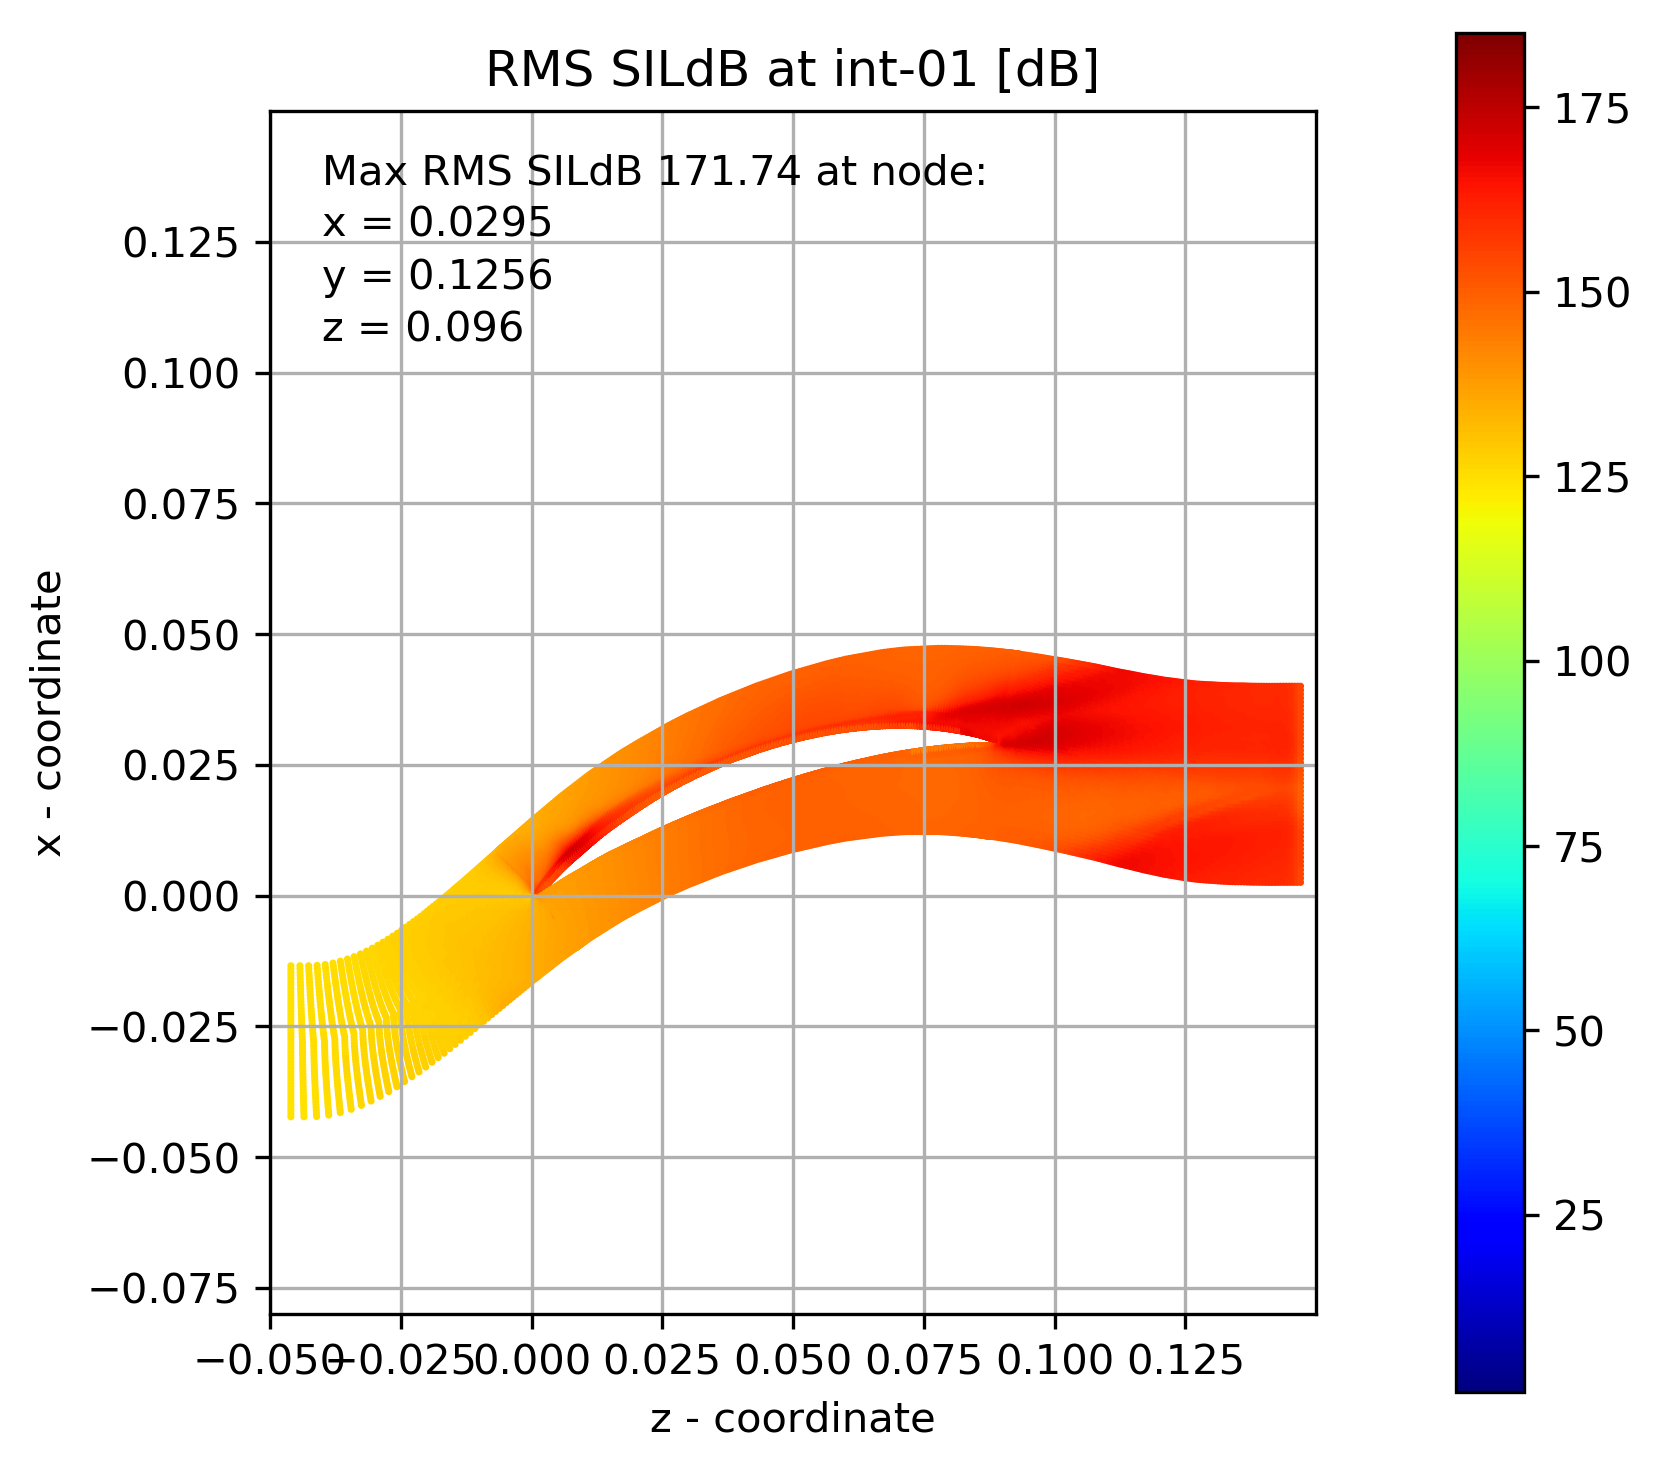
\includegraphics[width=0.75\textwidth]{Figures/int-01-rms-sildb.png} \label{int-01-rms-sildb}
  \caption{RMS Sound intensity decibel level at int-01 mark}
\end{figure}

%int-02
\begin{figure}[ht]
  \centering
  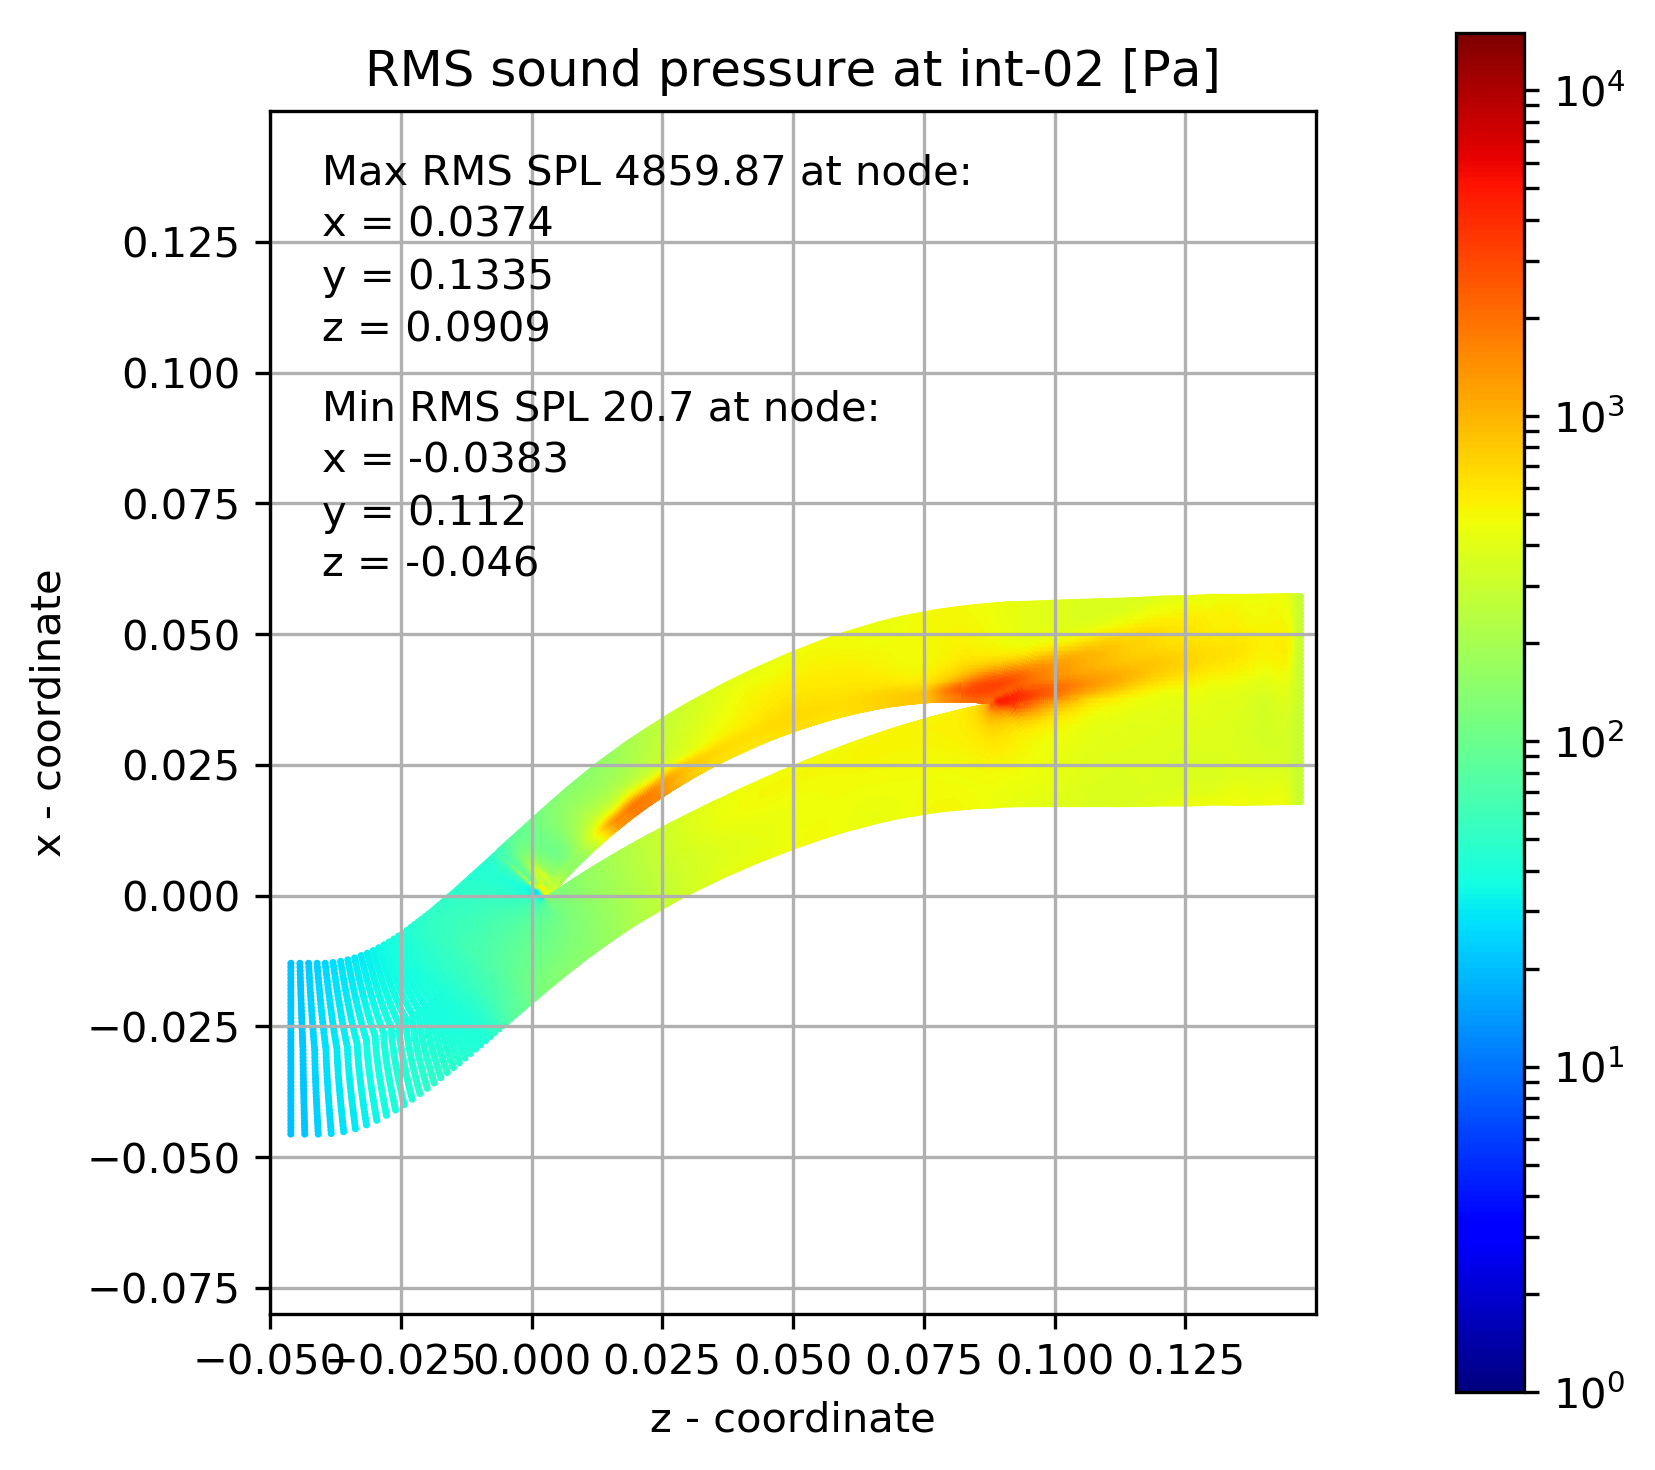
\includegraphics[width=0.75\textwidth]{Figures/int-02-rms-spl.png} \label{int-02-rms-spl}
  \caption{RMS Sound pressure at int-02 mark}
  
  \vspace*{\floatsep}% https://tex.stackexchange.com/q/26521/5764

  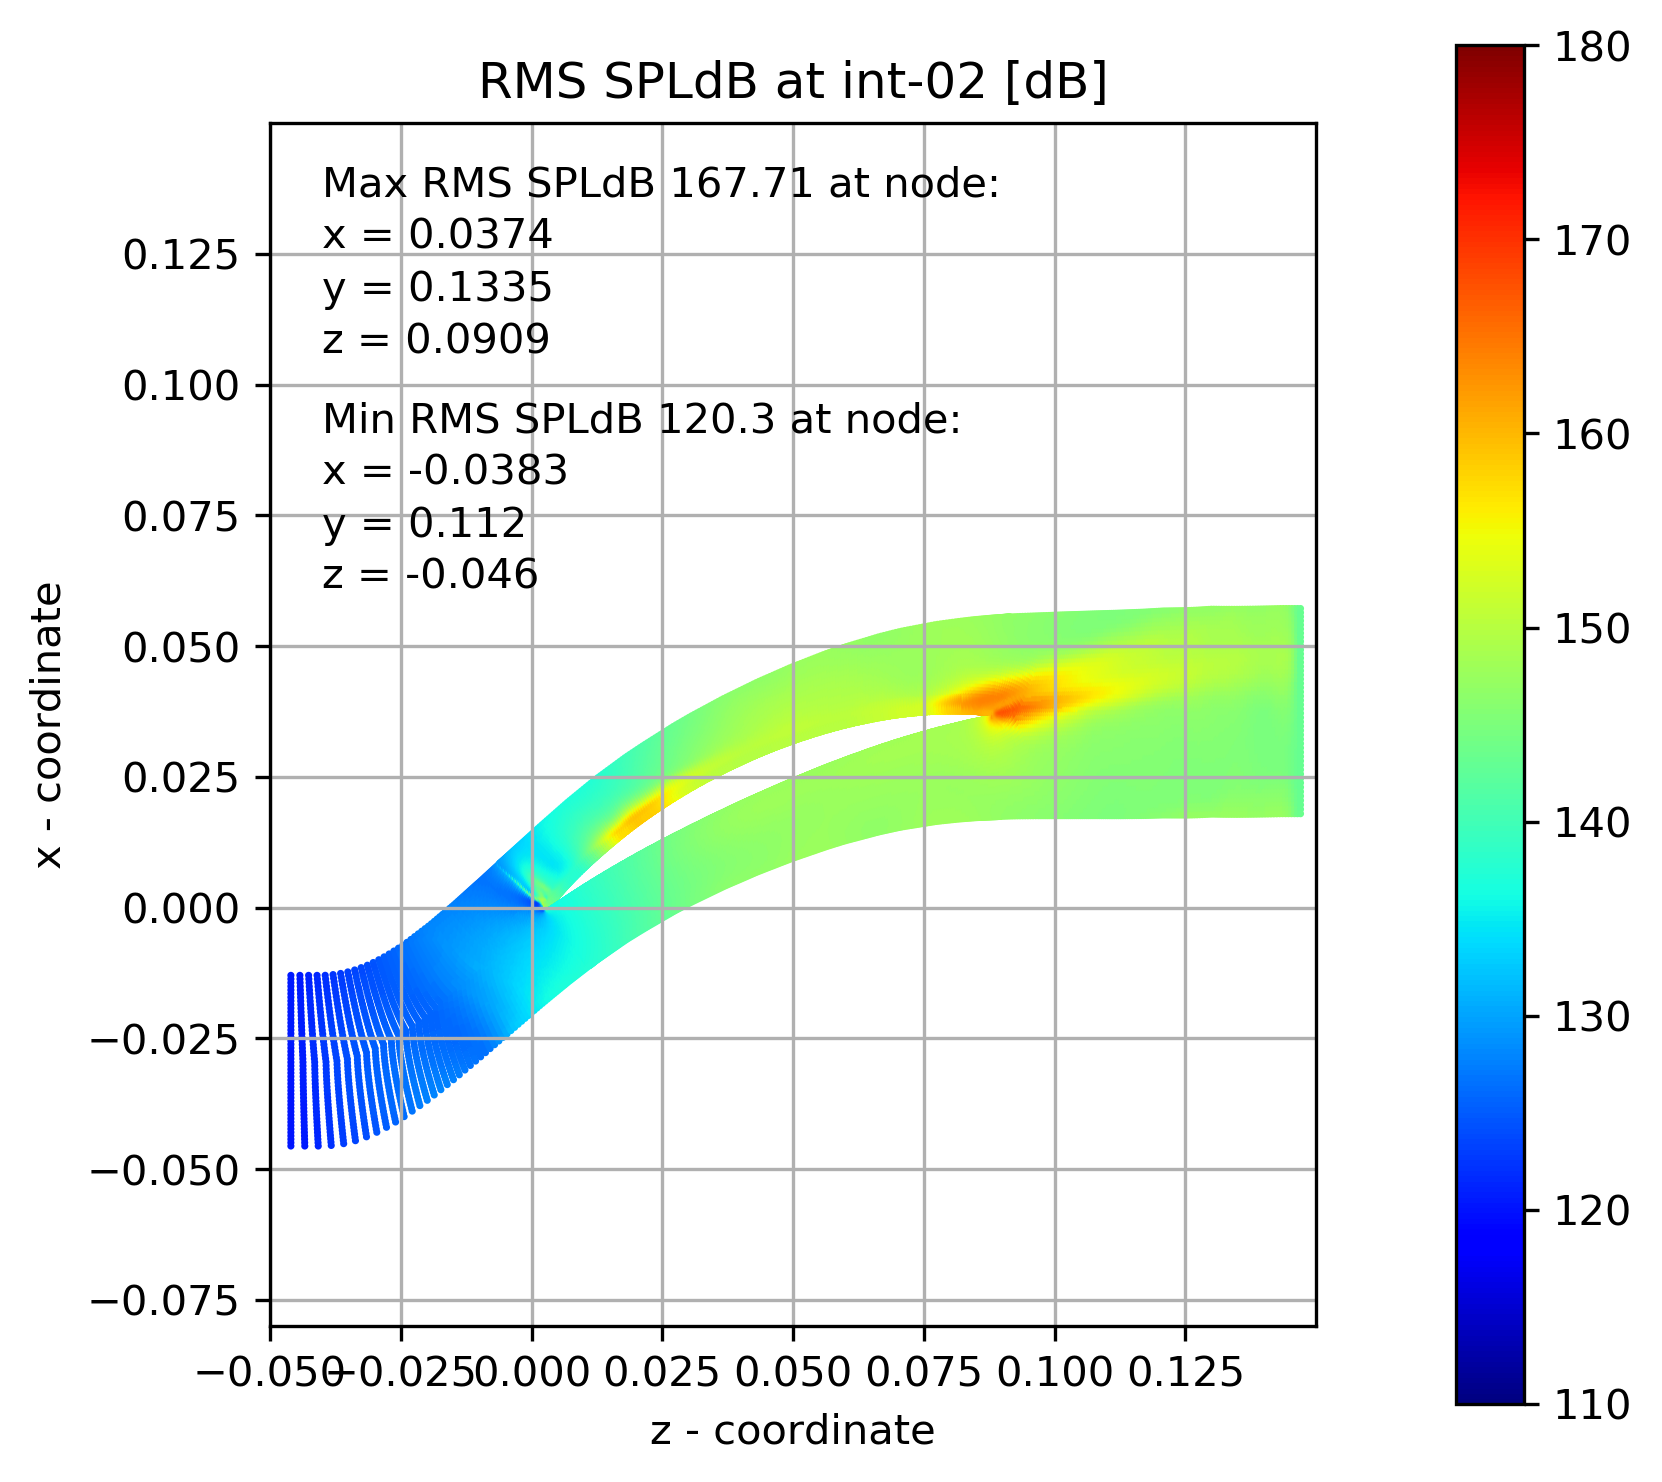
\includegraphics[width=0.75\textwidth]{Figures/int-02-rms-spldb.png} \label{int-02-rms-spldb}
  \caption{RMS Sound pressure decibel level at int-02 mark}
\end{figure}
%int-02
\begin{figure}[ht]
  \centering
  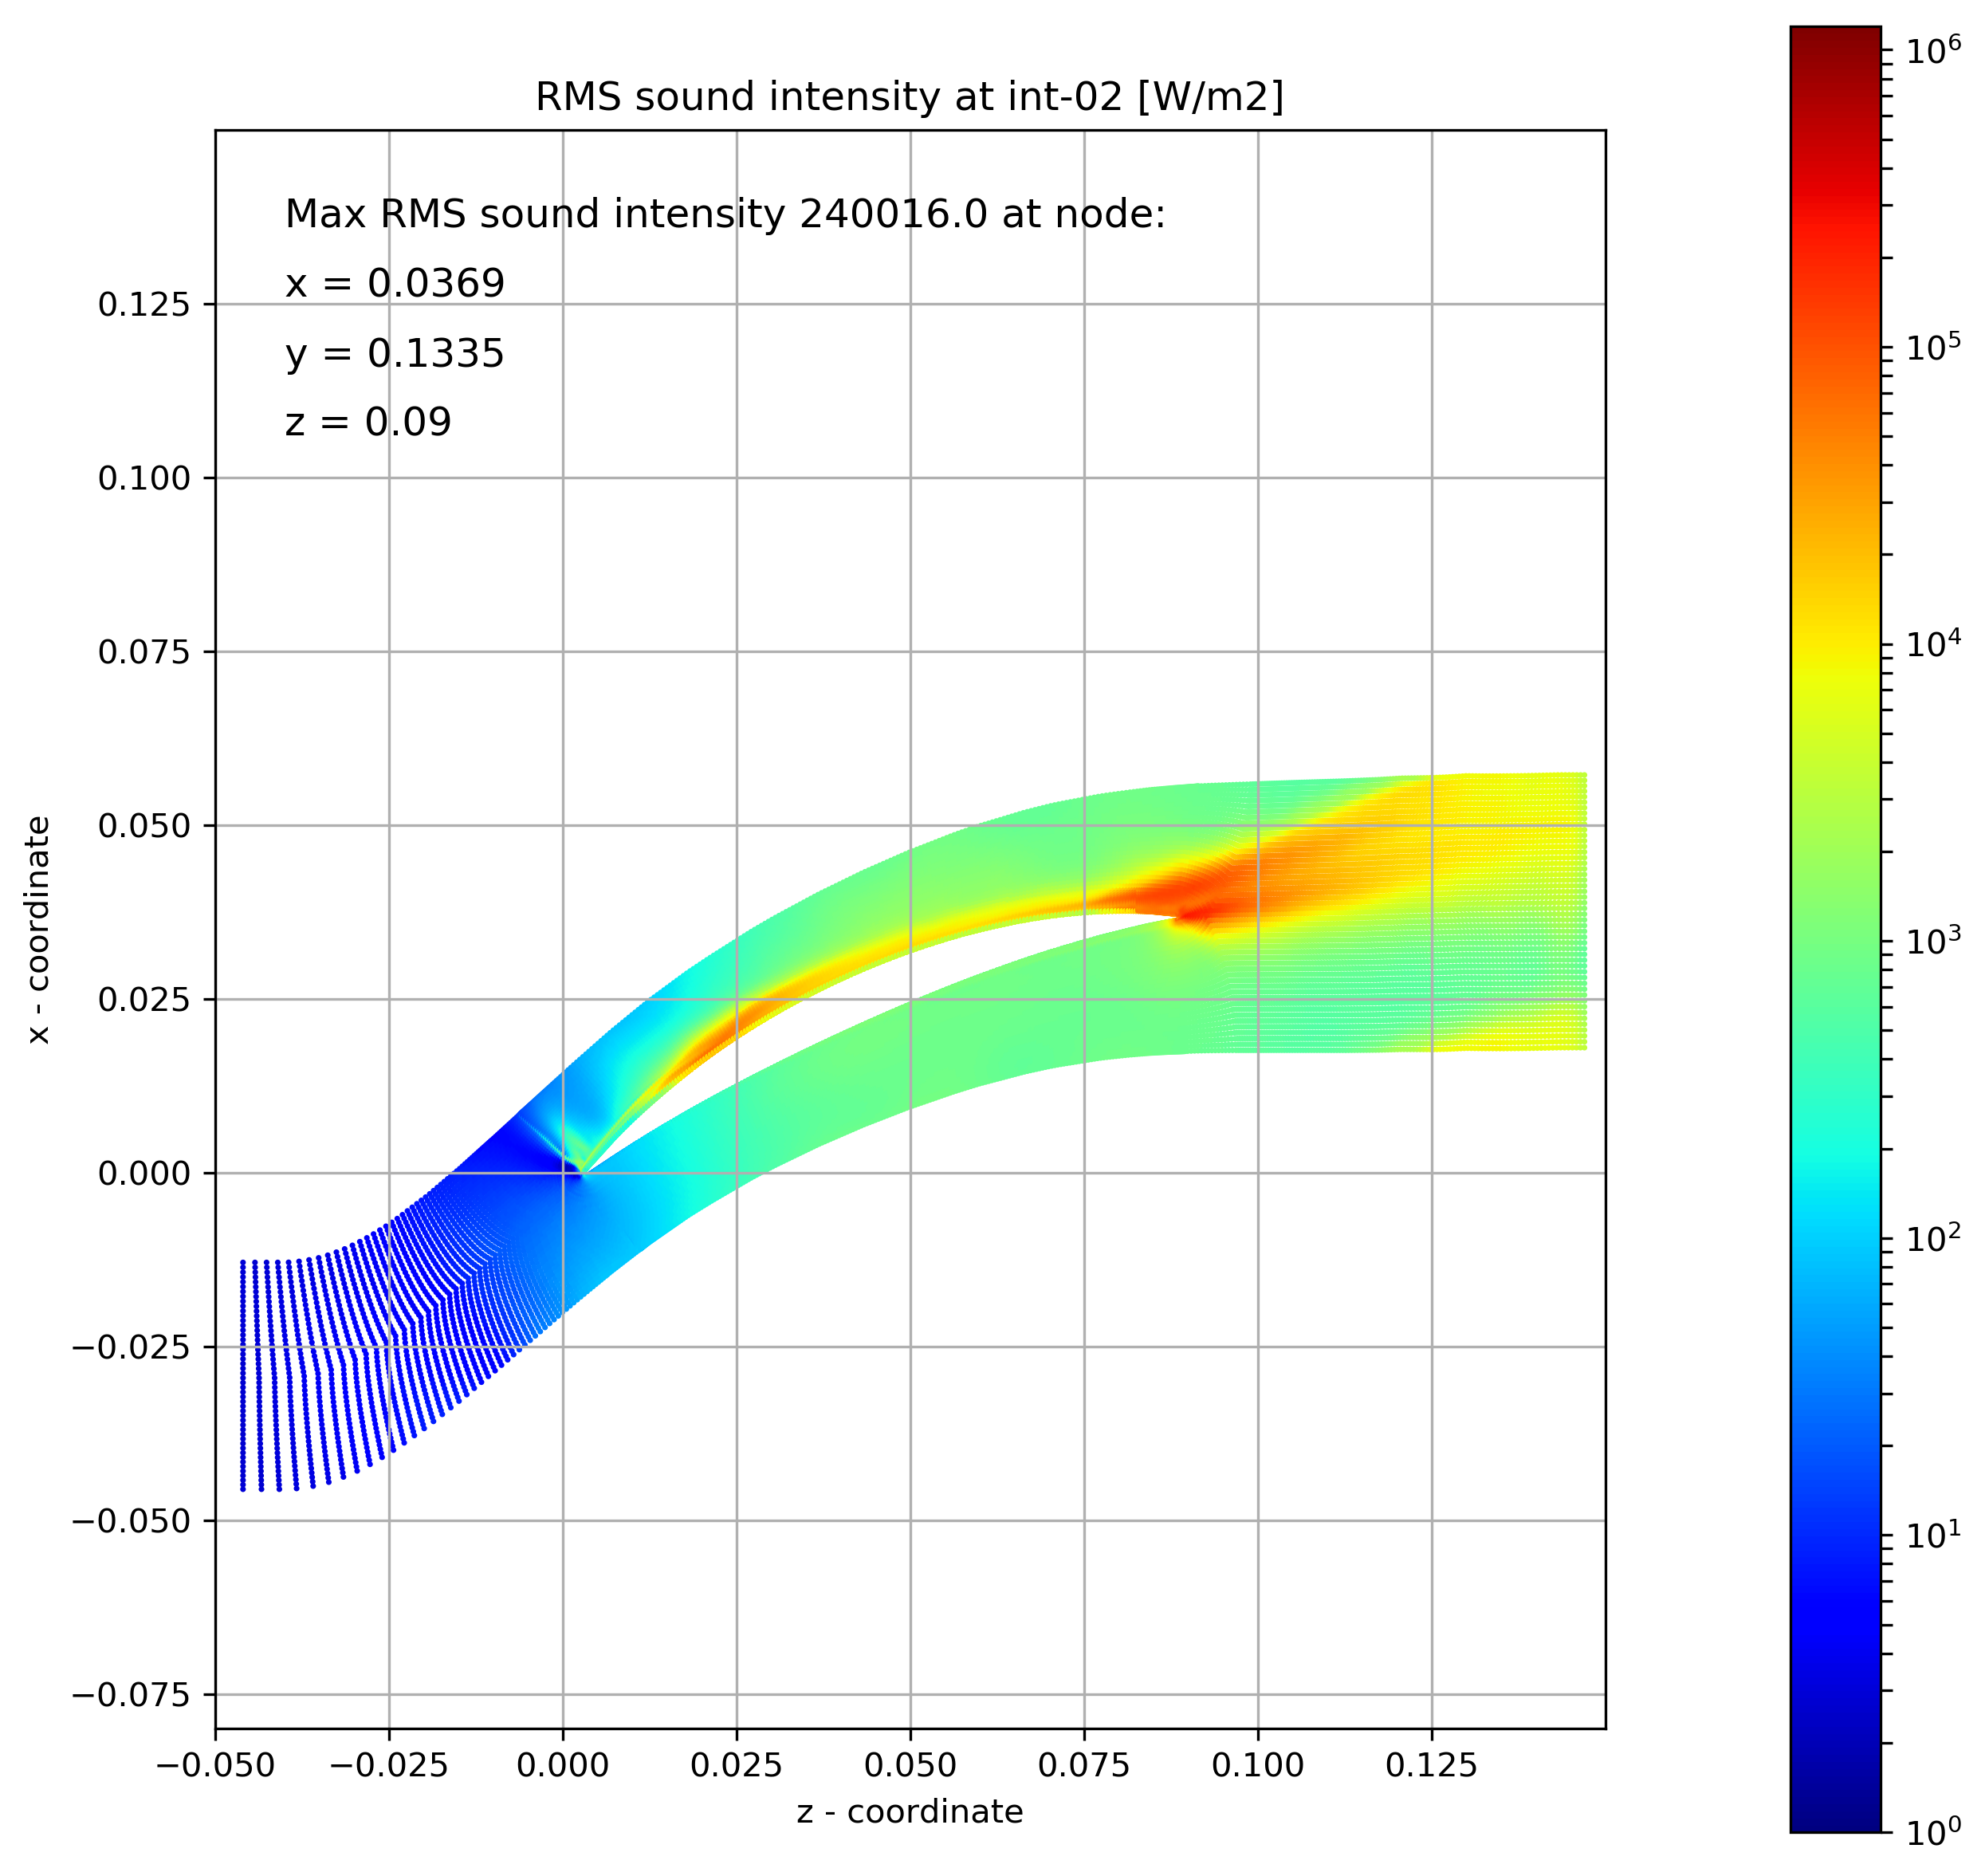
\includegraphics[width=0.75\textwidth]{Figures/int-02-rms-sil.png} \label{int-02-rms-sil}
  \caption{RMS Sound intensity at int-02 mark}
  
  \vspace*{\floatsep}% https://tex.stackexchange.com/q/26521/5764

  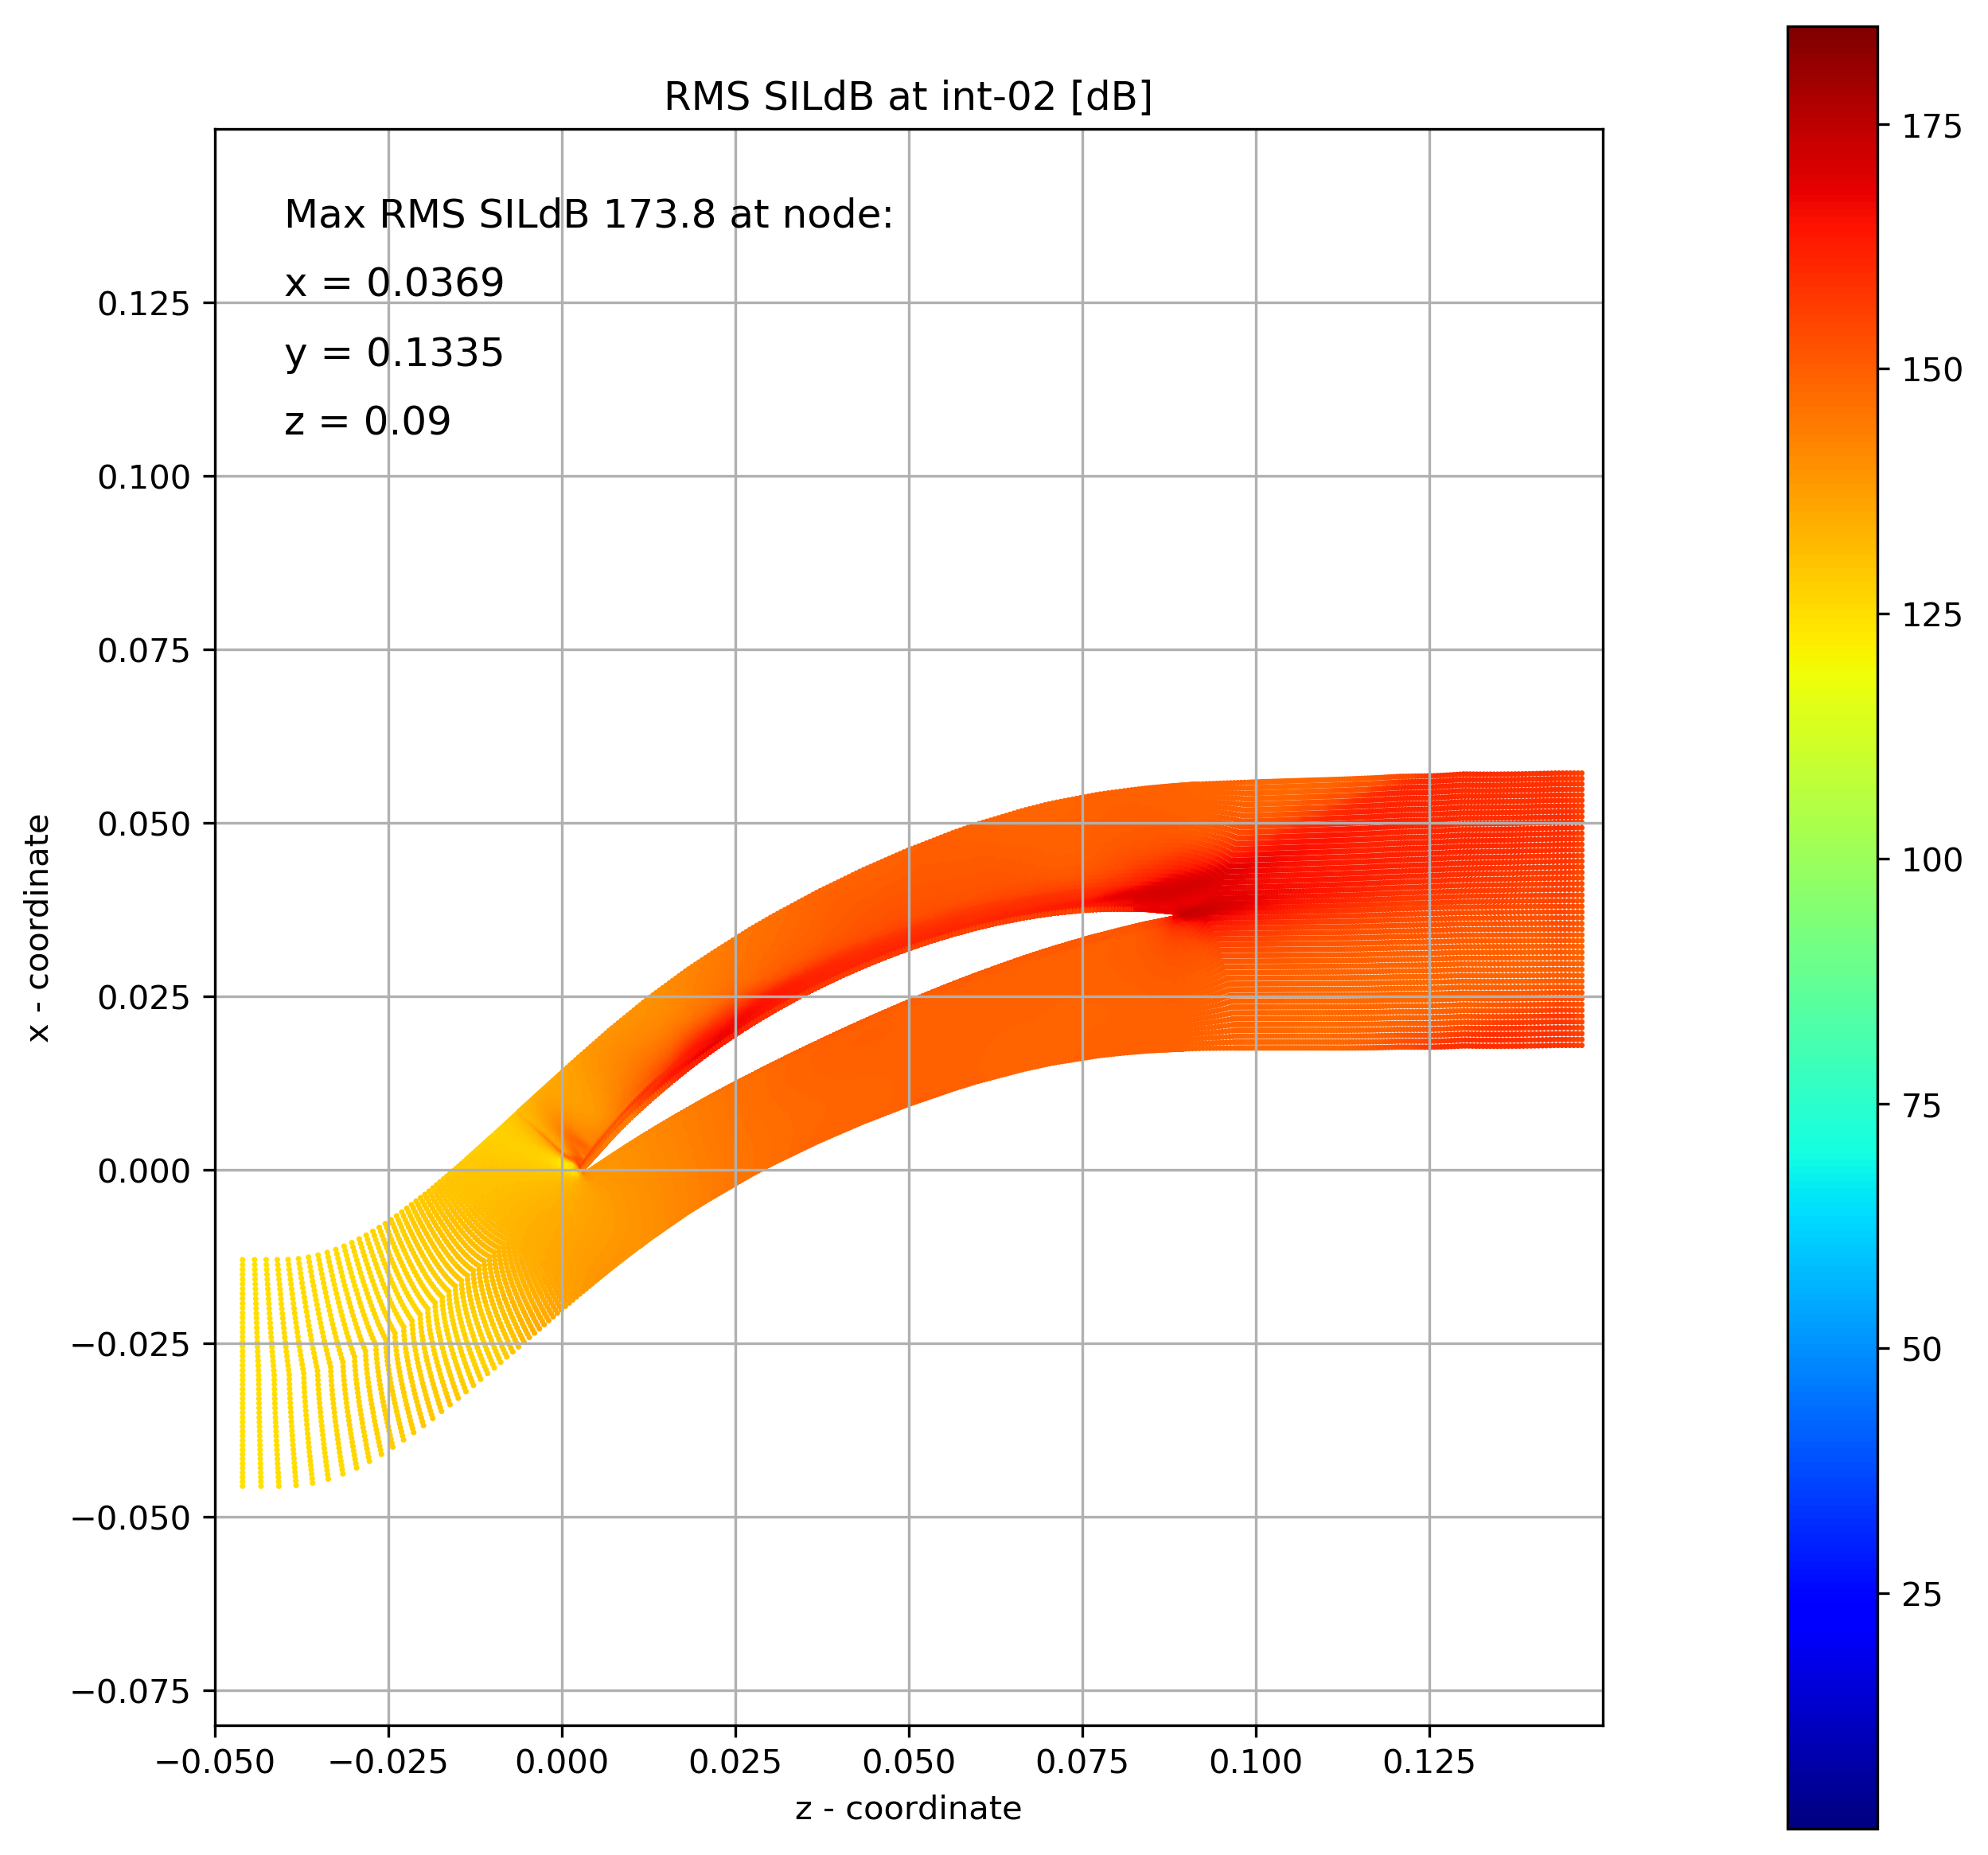
\includegraphics[width=0.75\textwidth]{Figures/int-02-rms-sildb.png} \label{int-02-rms-sildb}
  \caption{RMS Sound intensity decibel level at int-02 mark}
\end{figure}

%int-03
\begin{figure}[ht]
  \centering
  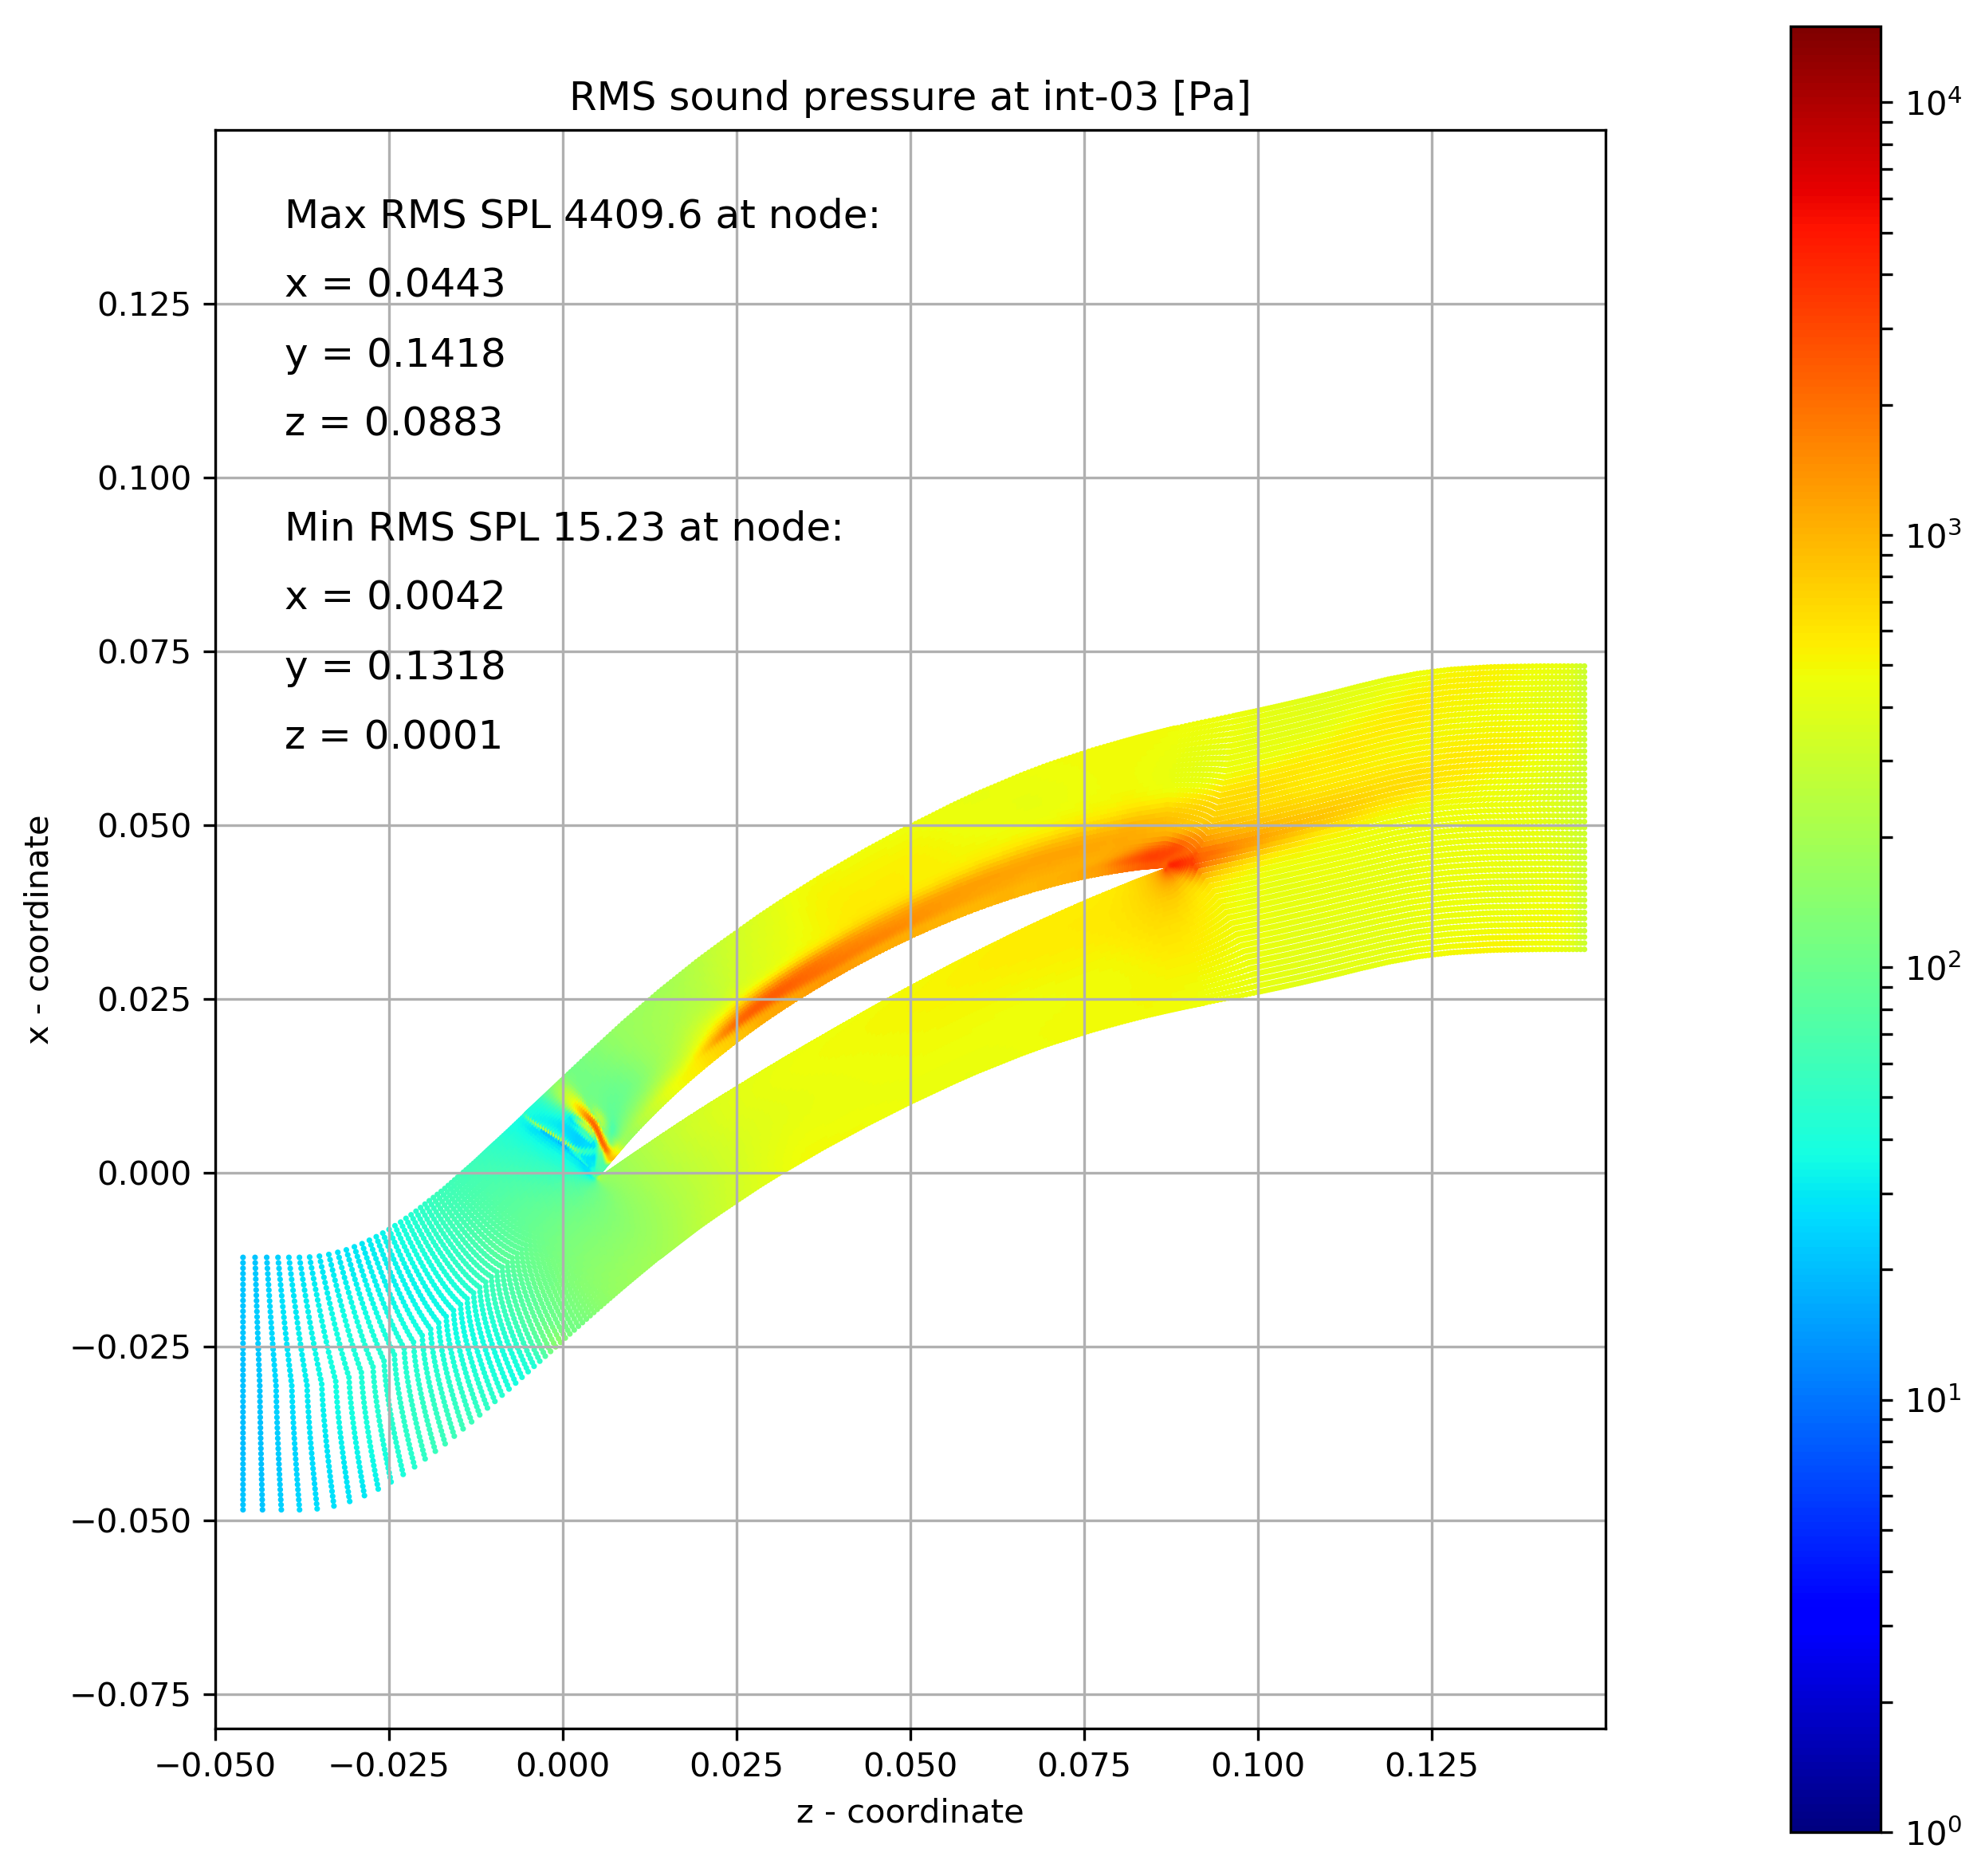
\includegraphics[width=0.75\textwidth]{Figures/int-03-rms-spl.png} \label{int-03-rms-spl}
  \caption{RMS Sound pressure at int-03 mark}
  
  \vspace*{\floatsep}% https://tex.stackexchange.com/q/26521/5764

  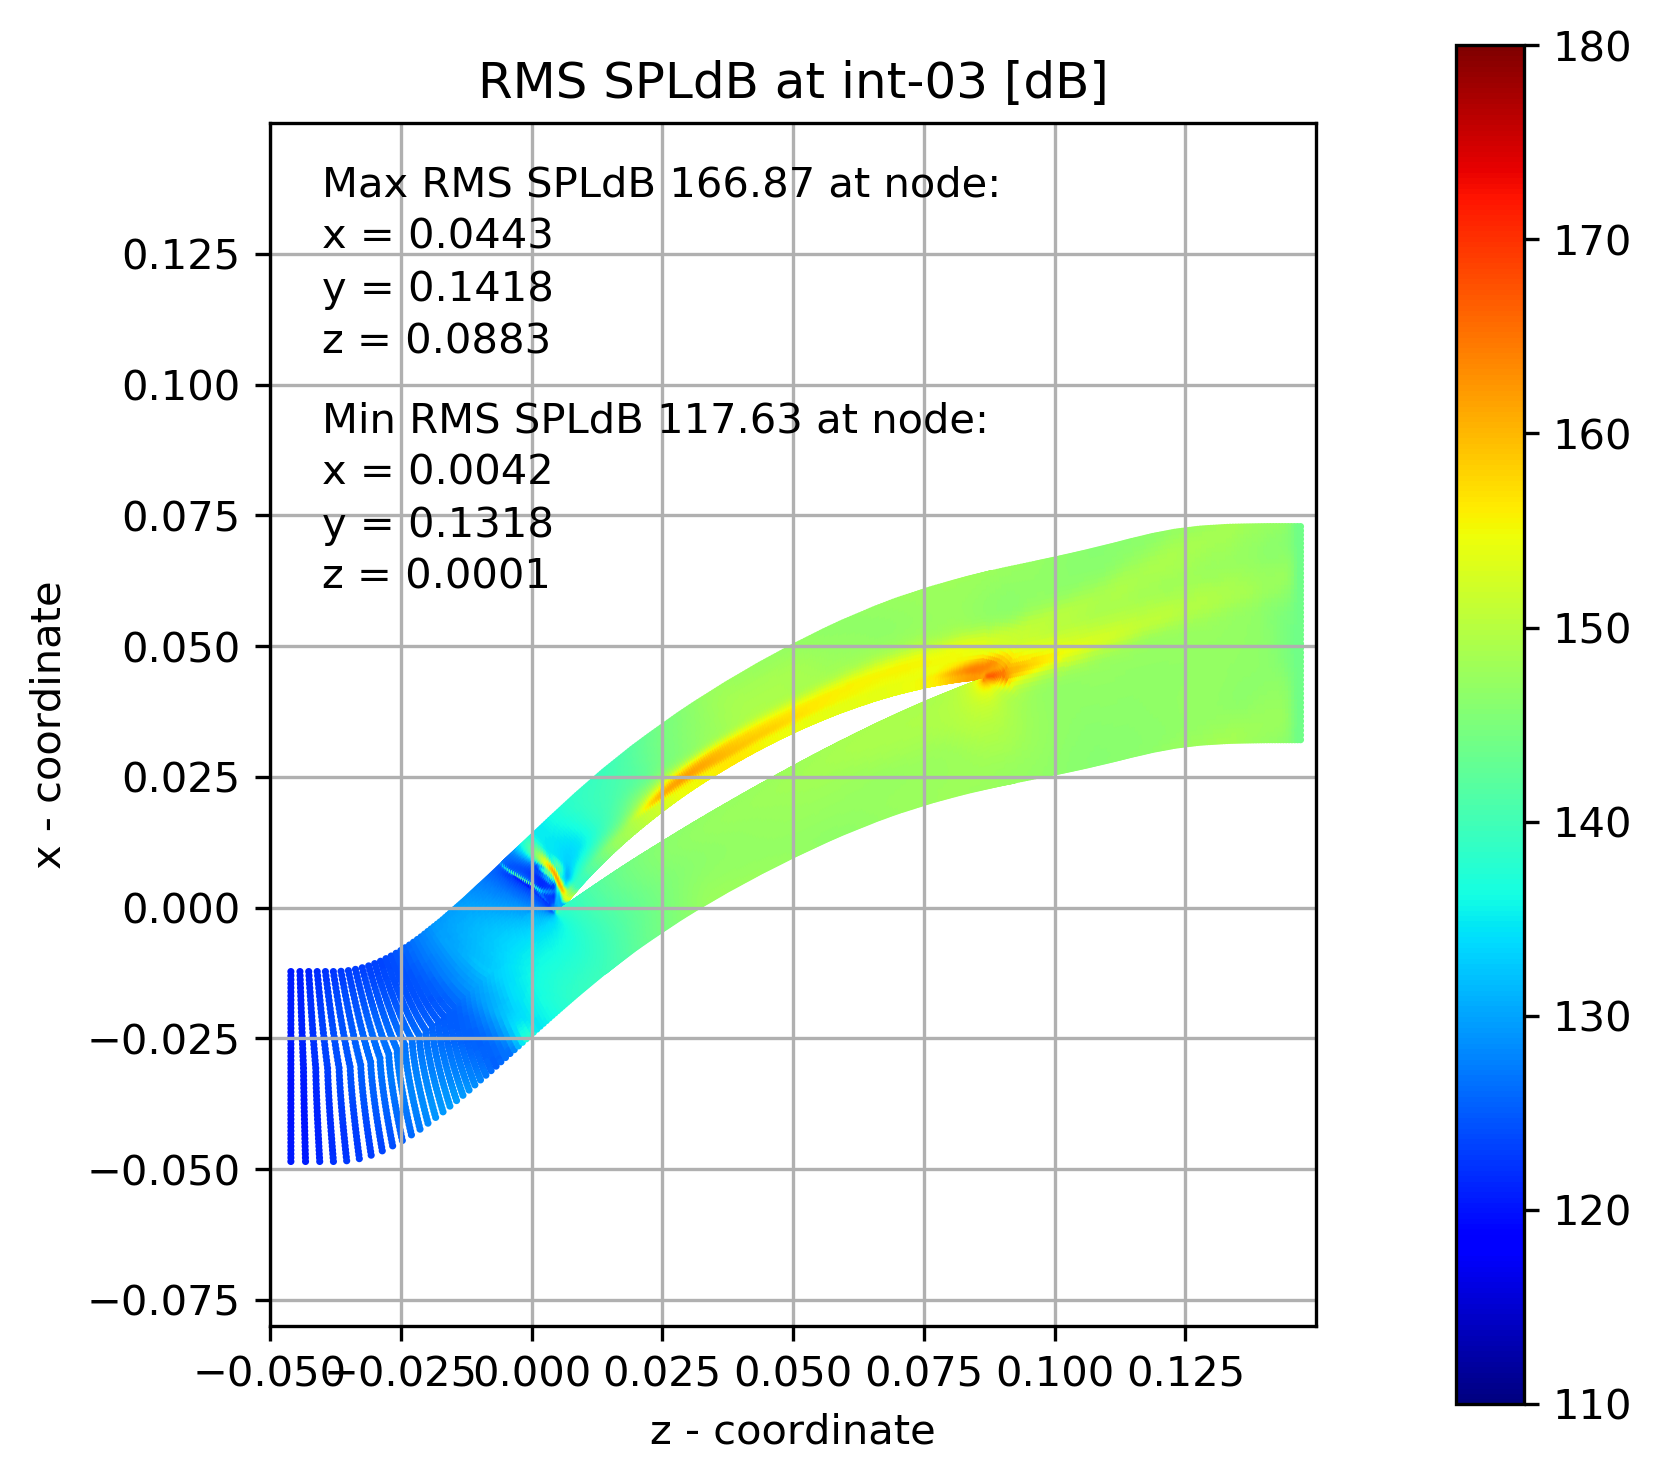
\includegraphics[width=0.75\textwidth]{Figures/int-03-rms-spldb.png} \label{int-03-rms-spldb}
  \caption{RMS Sound pressure decibel level at int-03 mark}
\end{figure}
%int-03
\begin{figure}[ht]
  \centering
  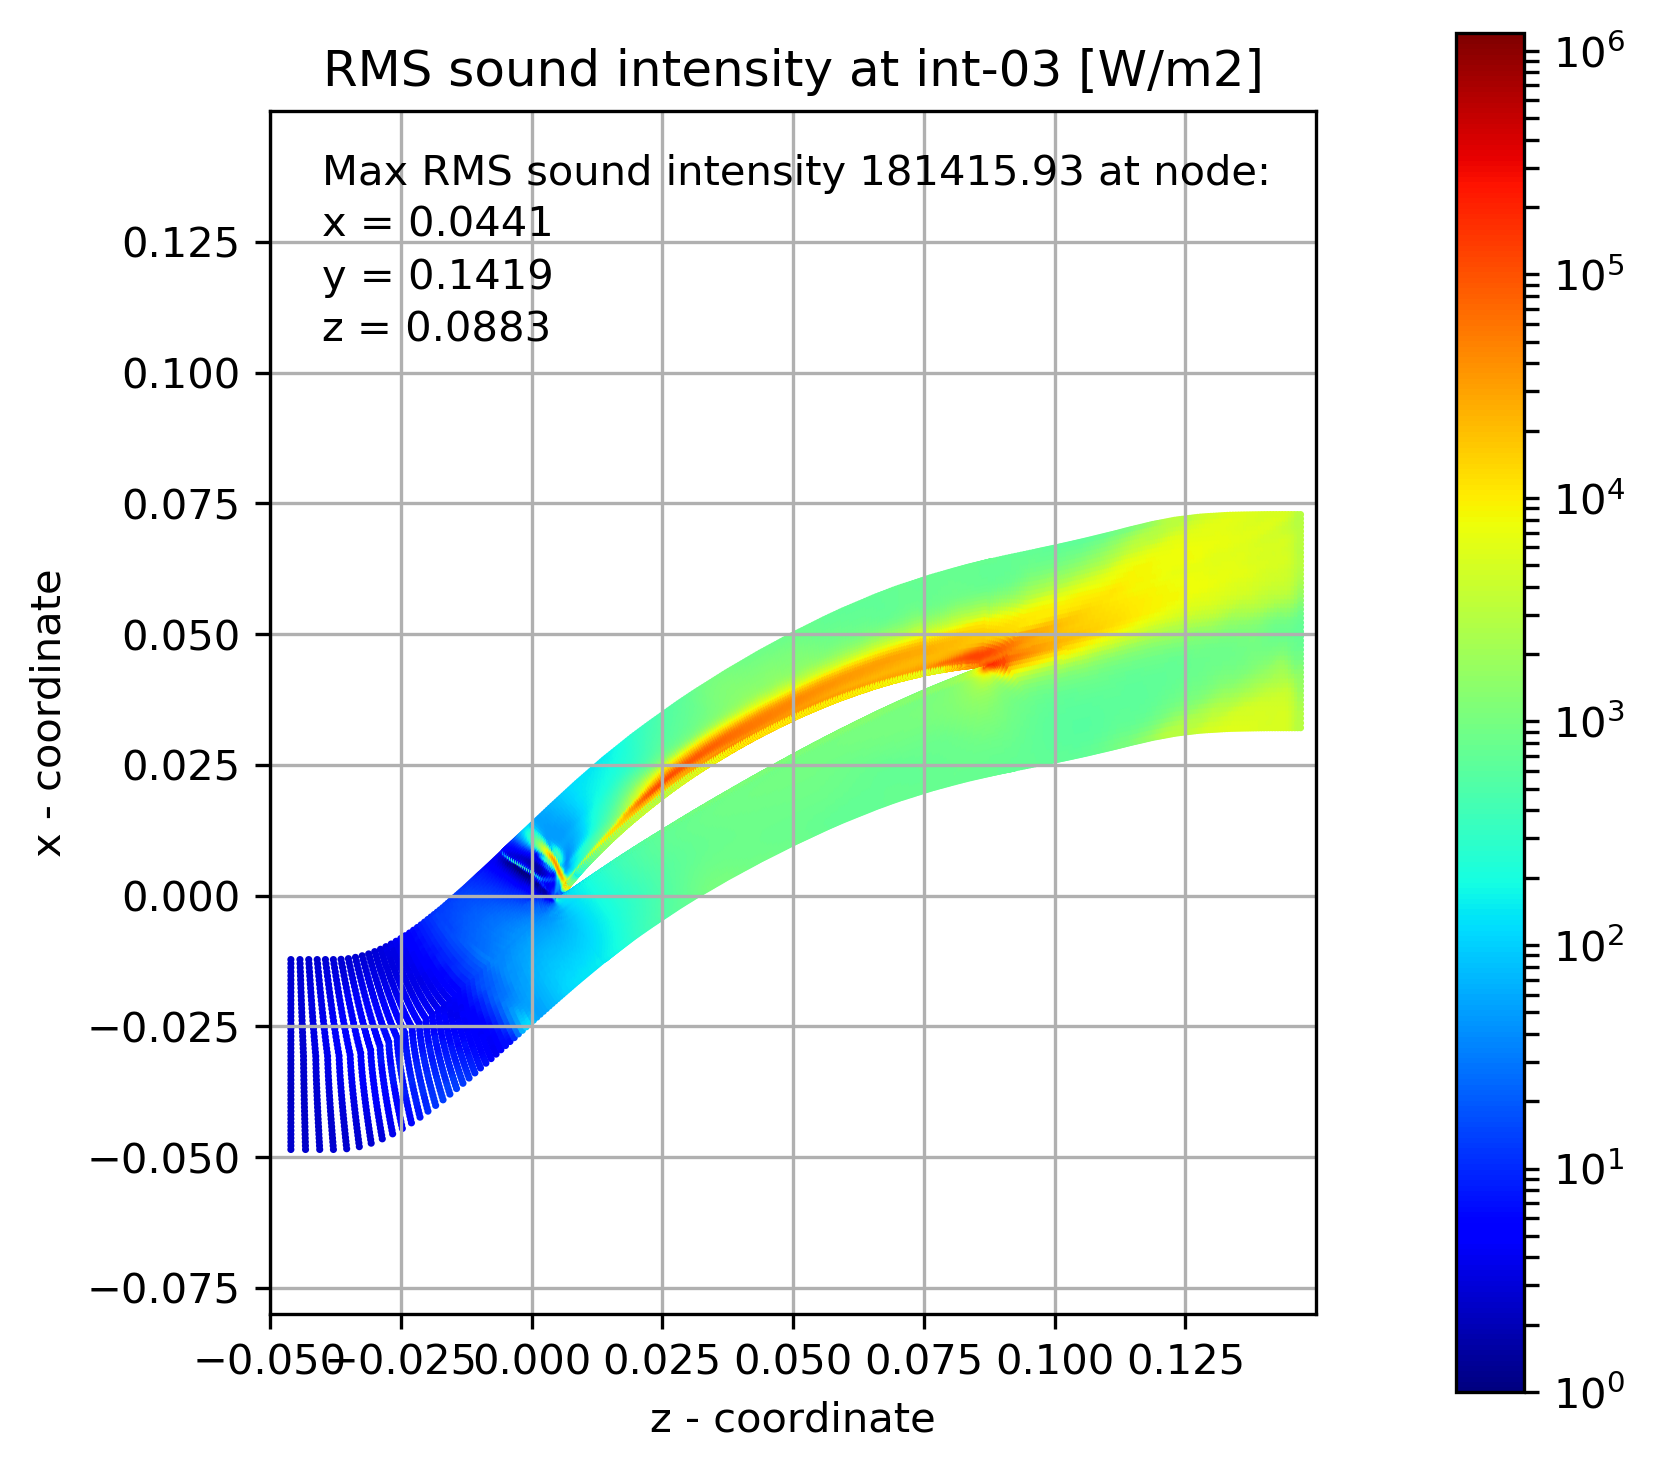
\includegraphics[width=0.75\textwidth]{Figures/int-03-rms-sil.png} \label{int-03-rms-sil}
  \caption{RMS Sound intensity at int-03 mark}
  
  \vspace*{\floatsep}% https://tex.stackexchange.com/q/26521/5764

  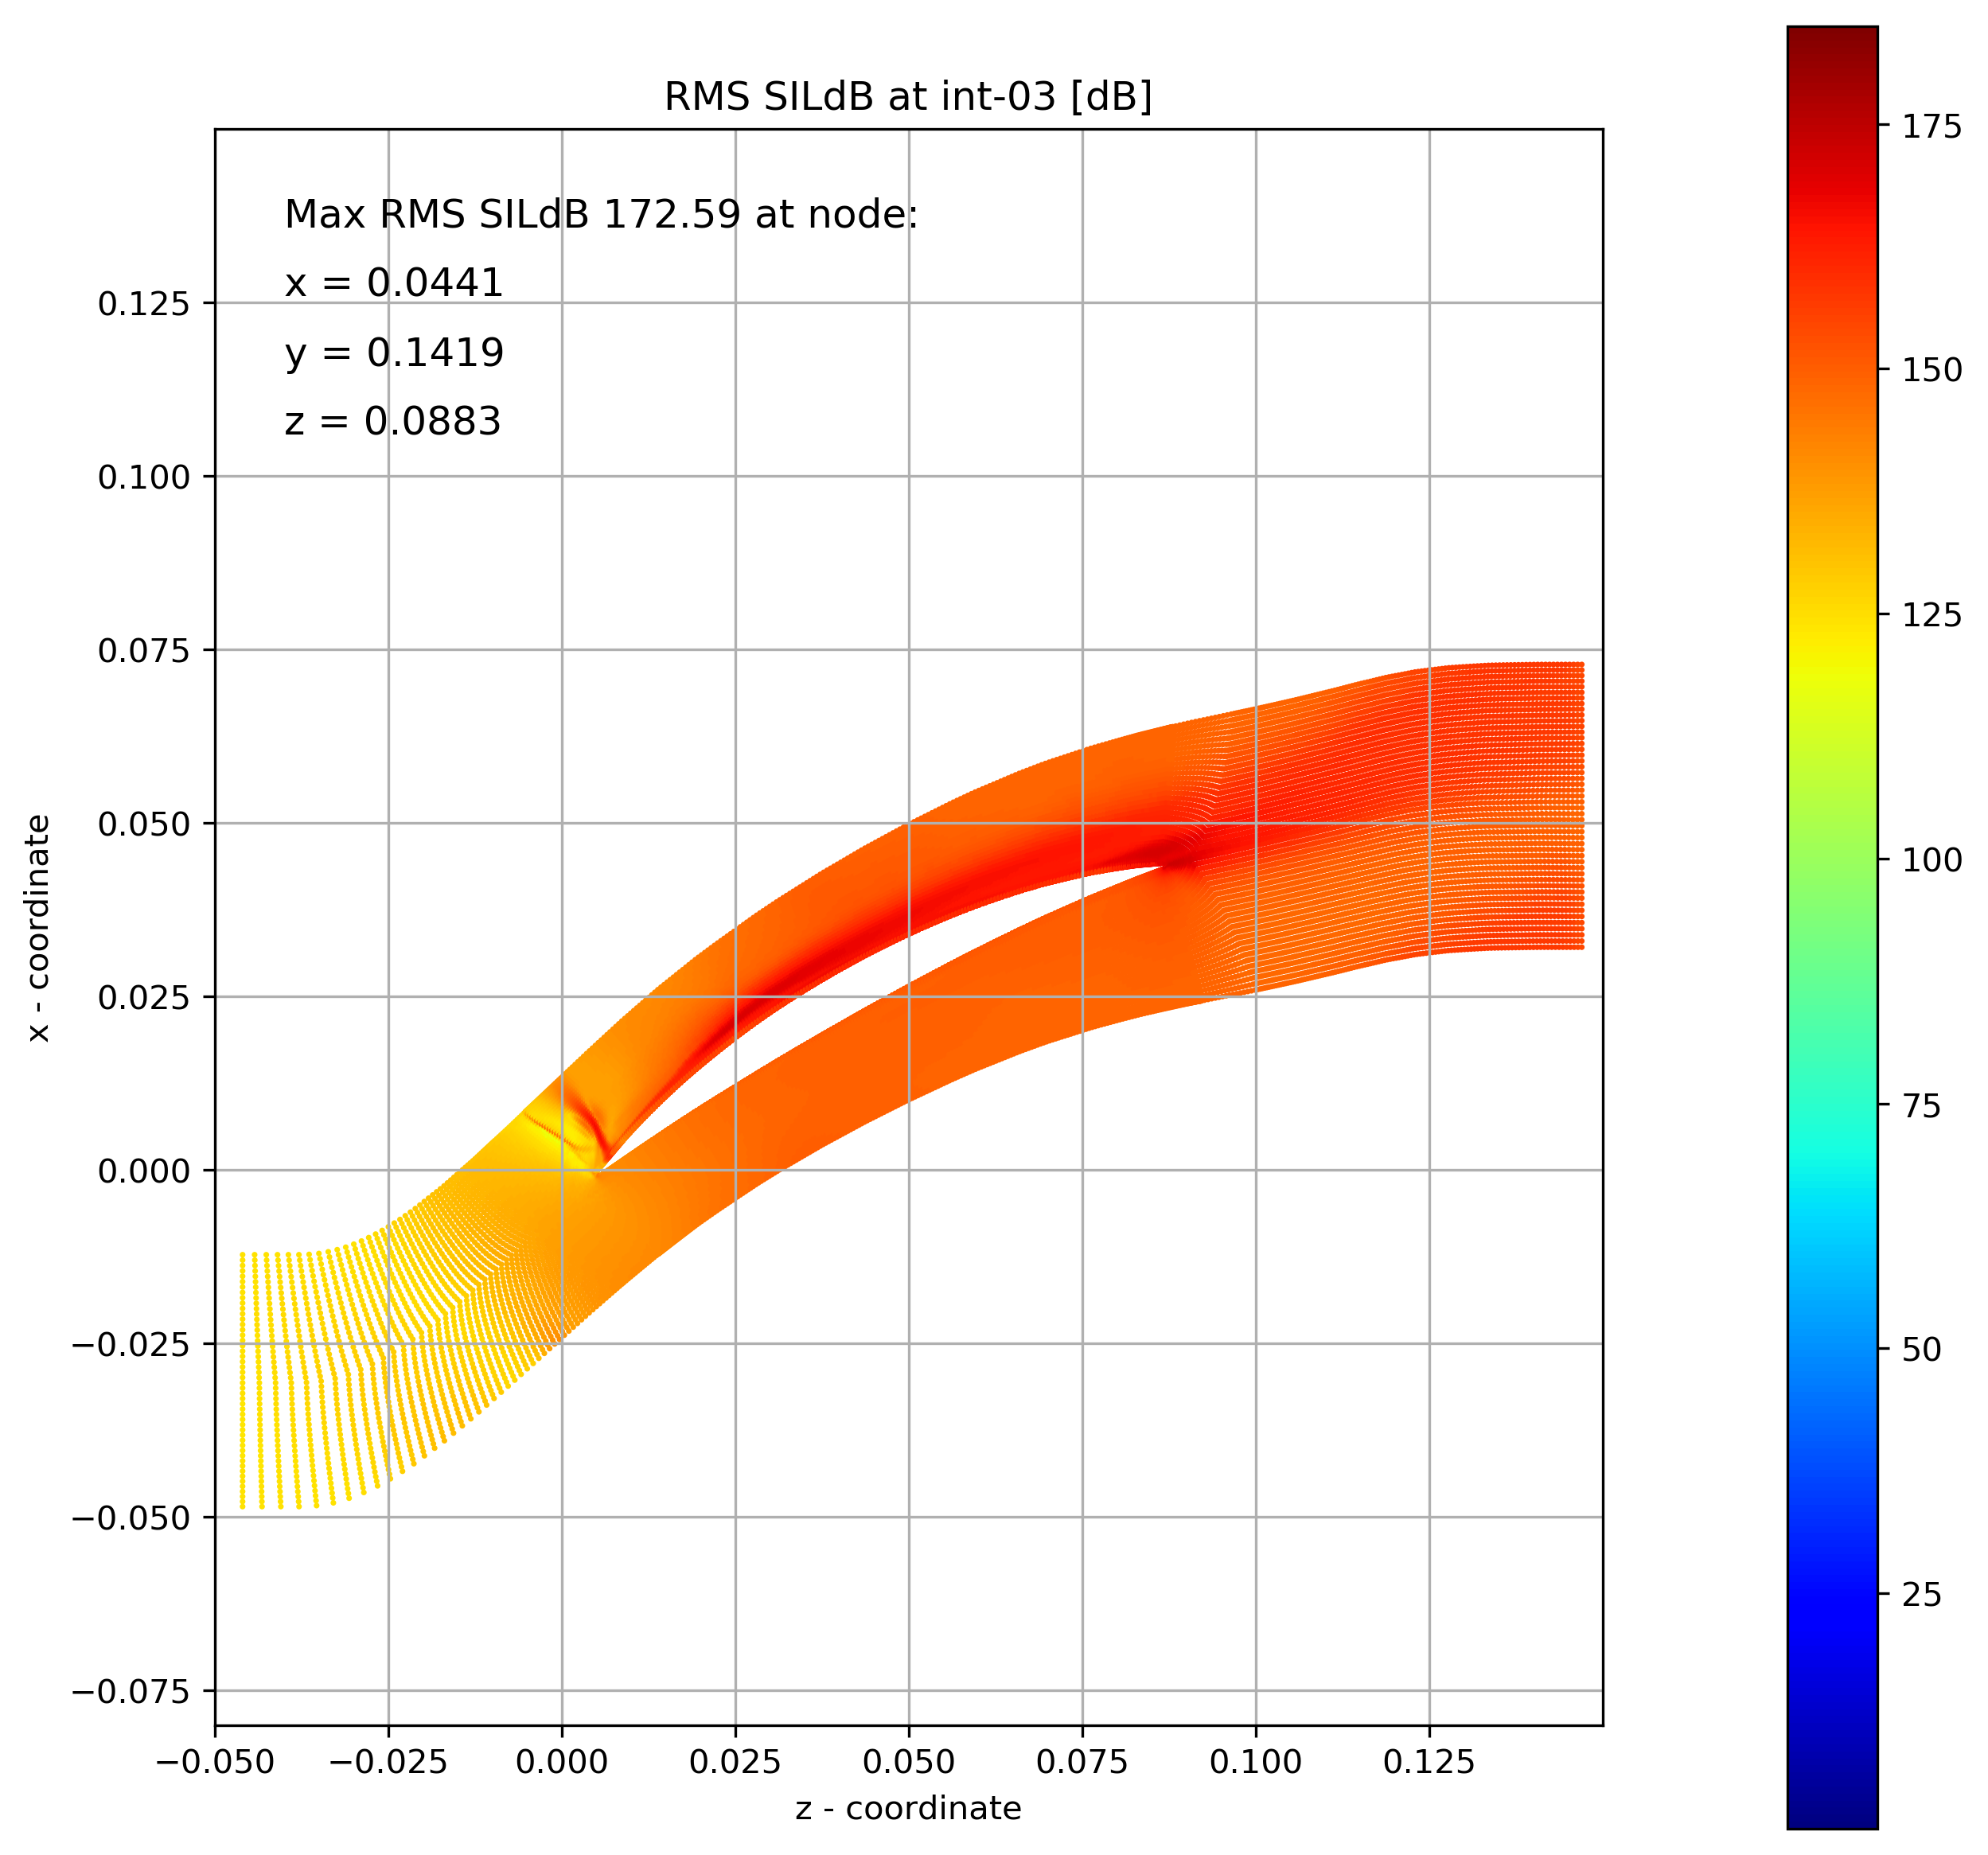
\includegraphics[width=0.75\textwidth]{Figures/int-03-rms-sildb.png} \label{int-03-rms-sildb}
  \caption{RMS Sound intensity decibel level at int-03 mark}
\end{figure}

%int-04
\begin{figure}[ht]
  \centering
  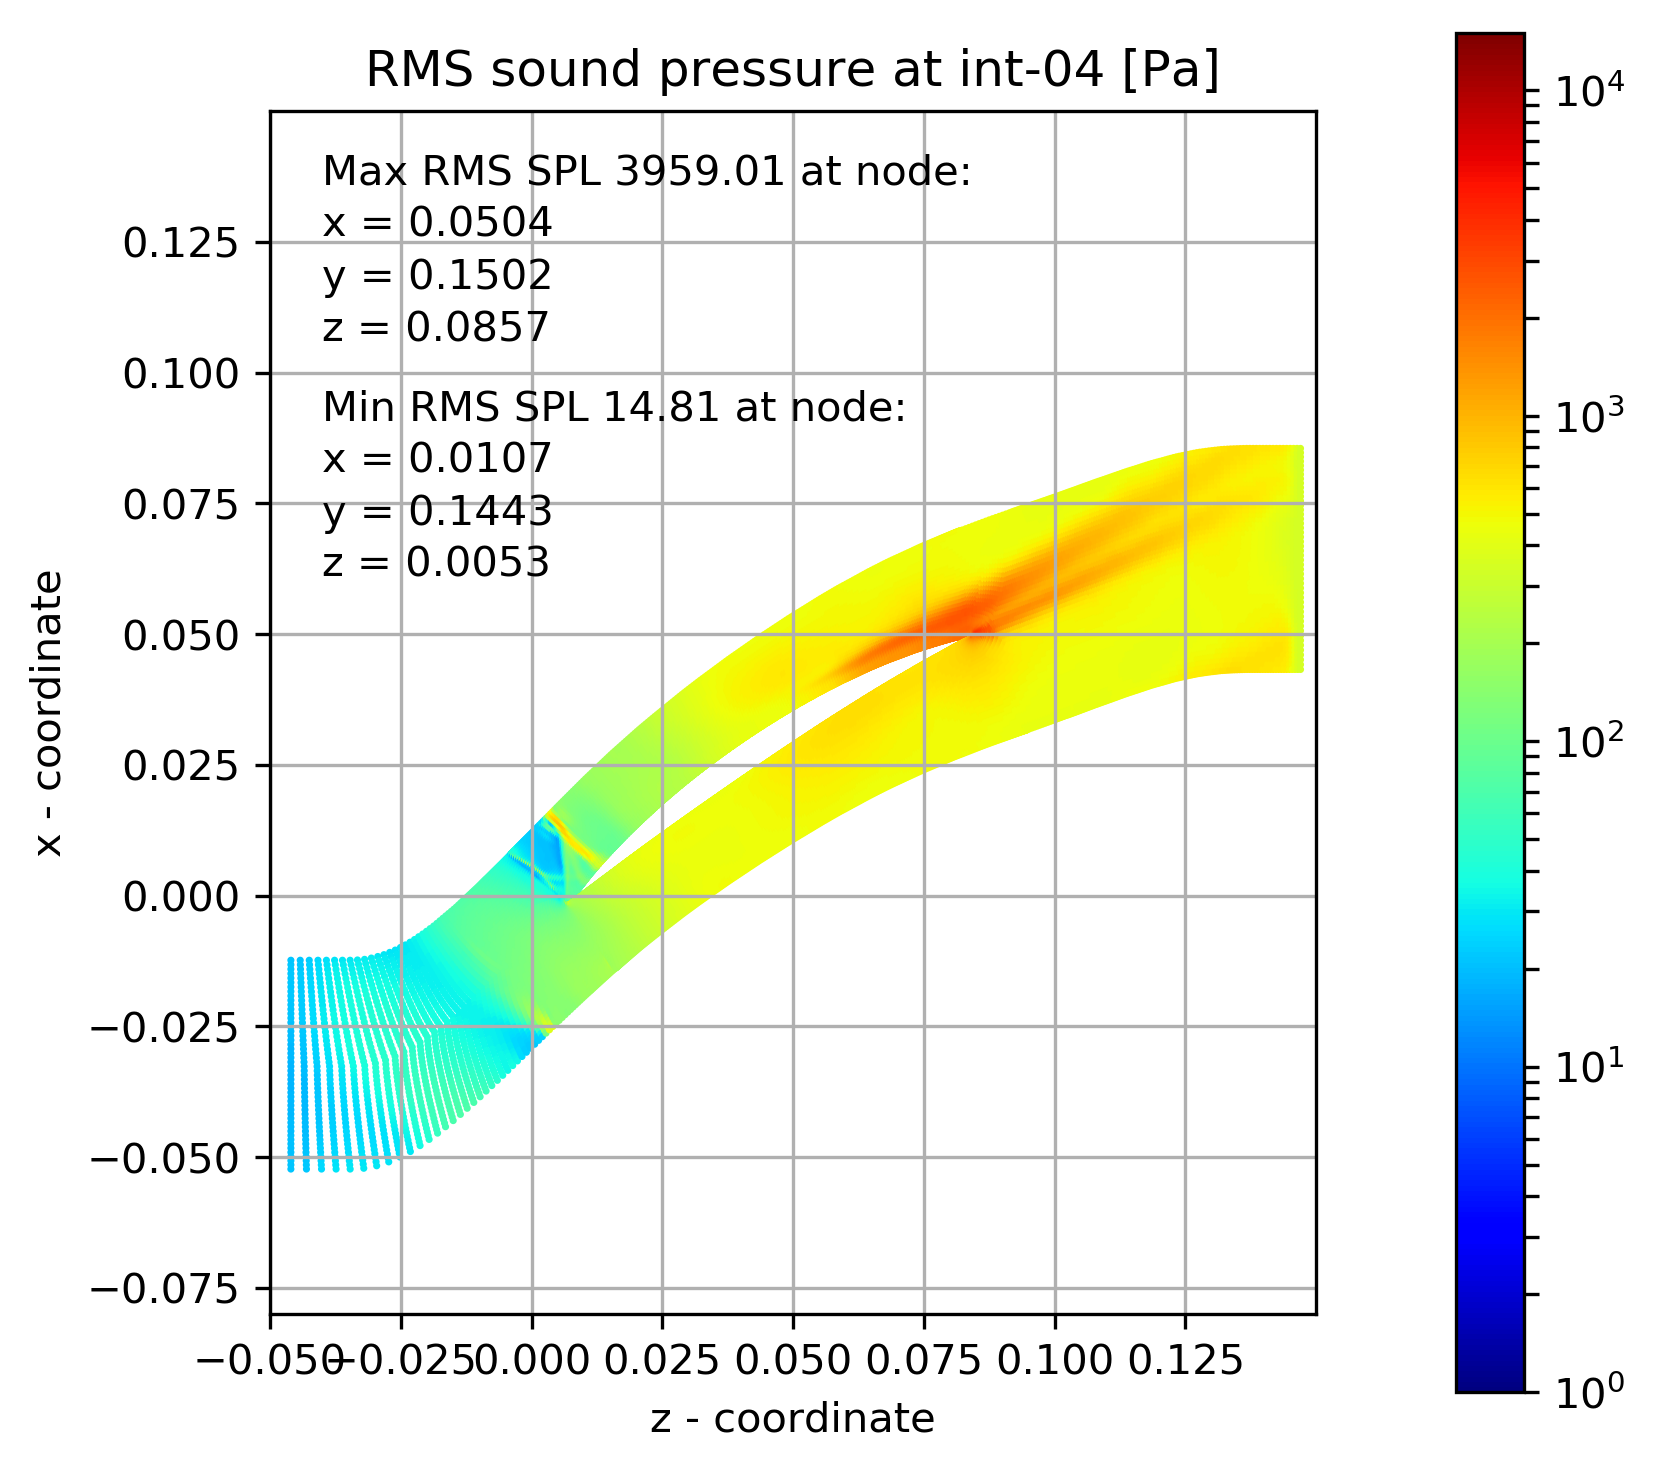
\includegraphics[width=0.75\textwidth]{Figures/int-04-rms-spl.png} \label{int-04-rms-spl}
  \caption{RMS Sound pressure at int-04 mark}
  
  \vspace*{\floatsep}% https://tex.stackexchange.com/q/26521/5764

  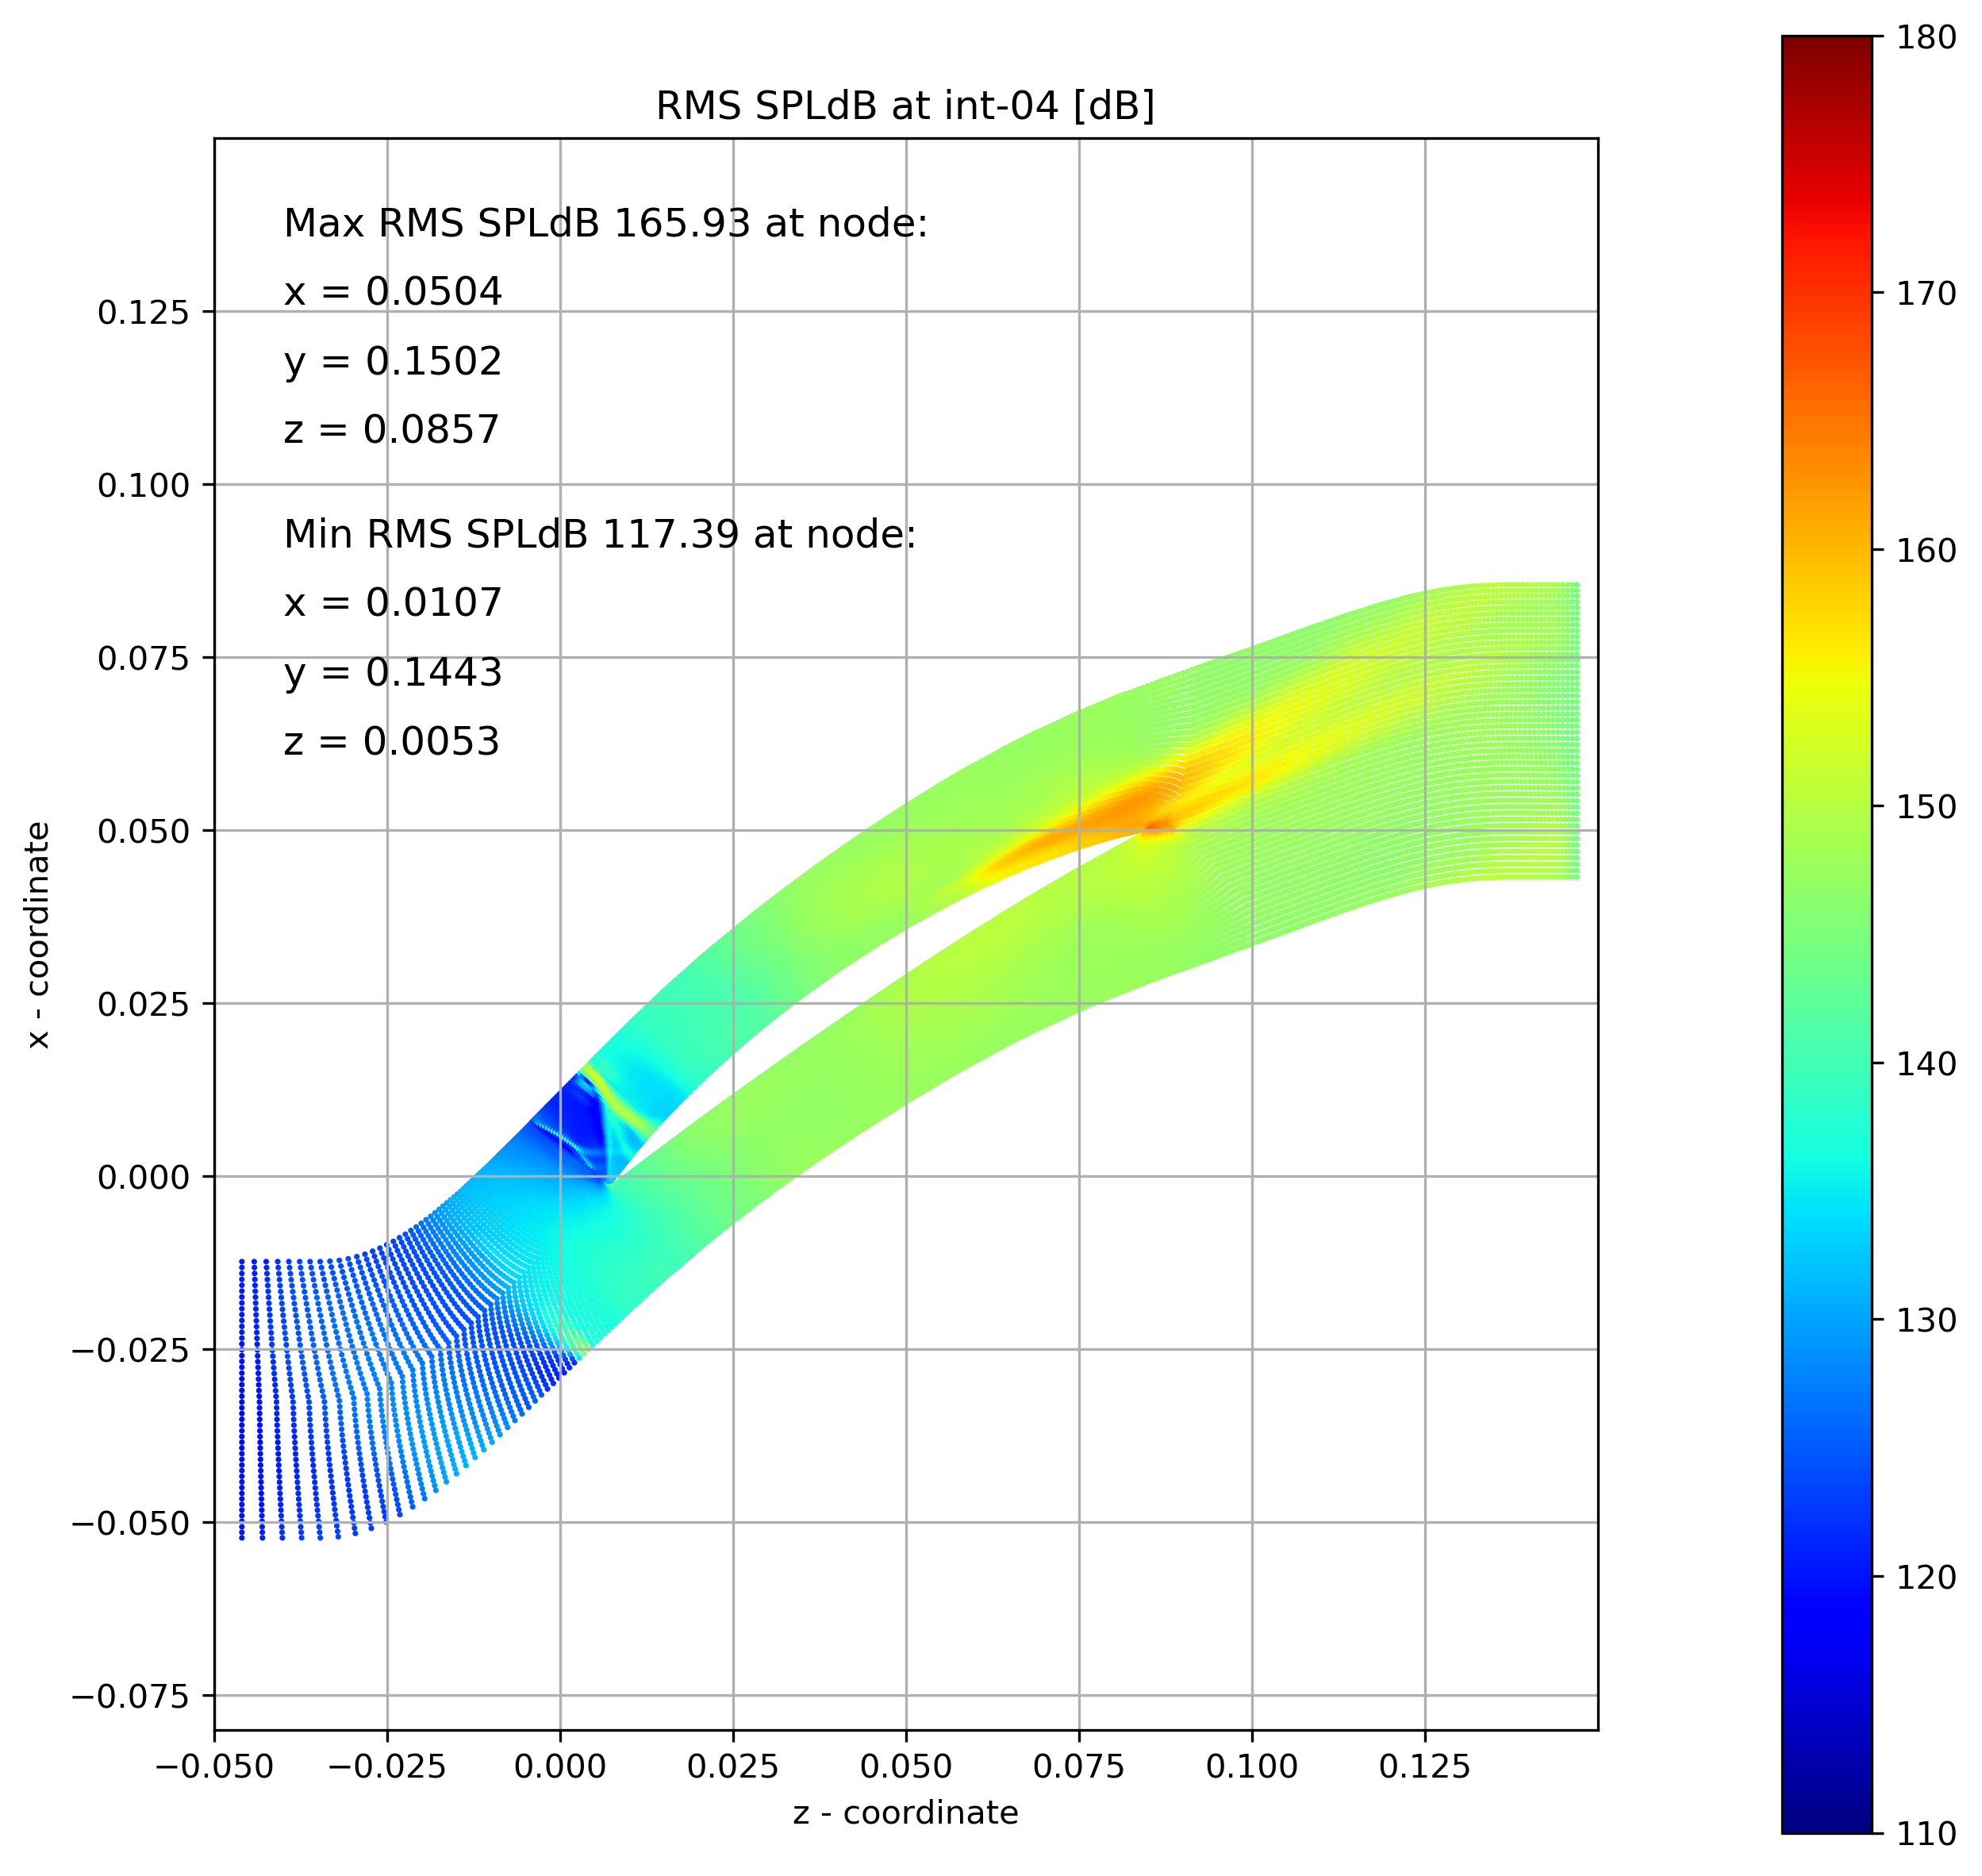
\includegraphics[width=0.75\textwidth]{Figures/int-04-rms-spldb.png} \label{int-04-rms-spldb}
  \caption{RMS Sound pressure decibel level at int-04 mark}
\end{figure}
%int-04
\begin{figure}[ht]
  \centering
  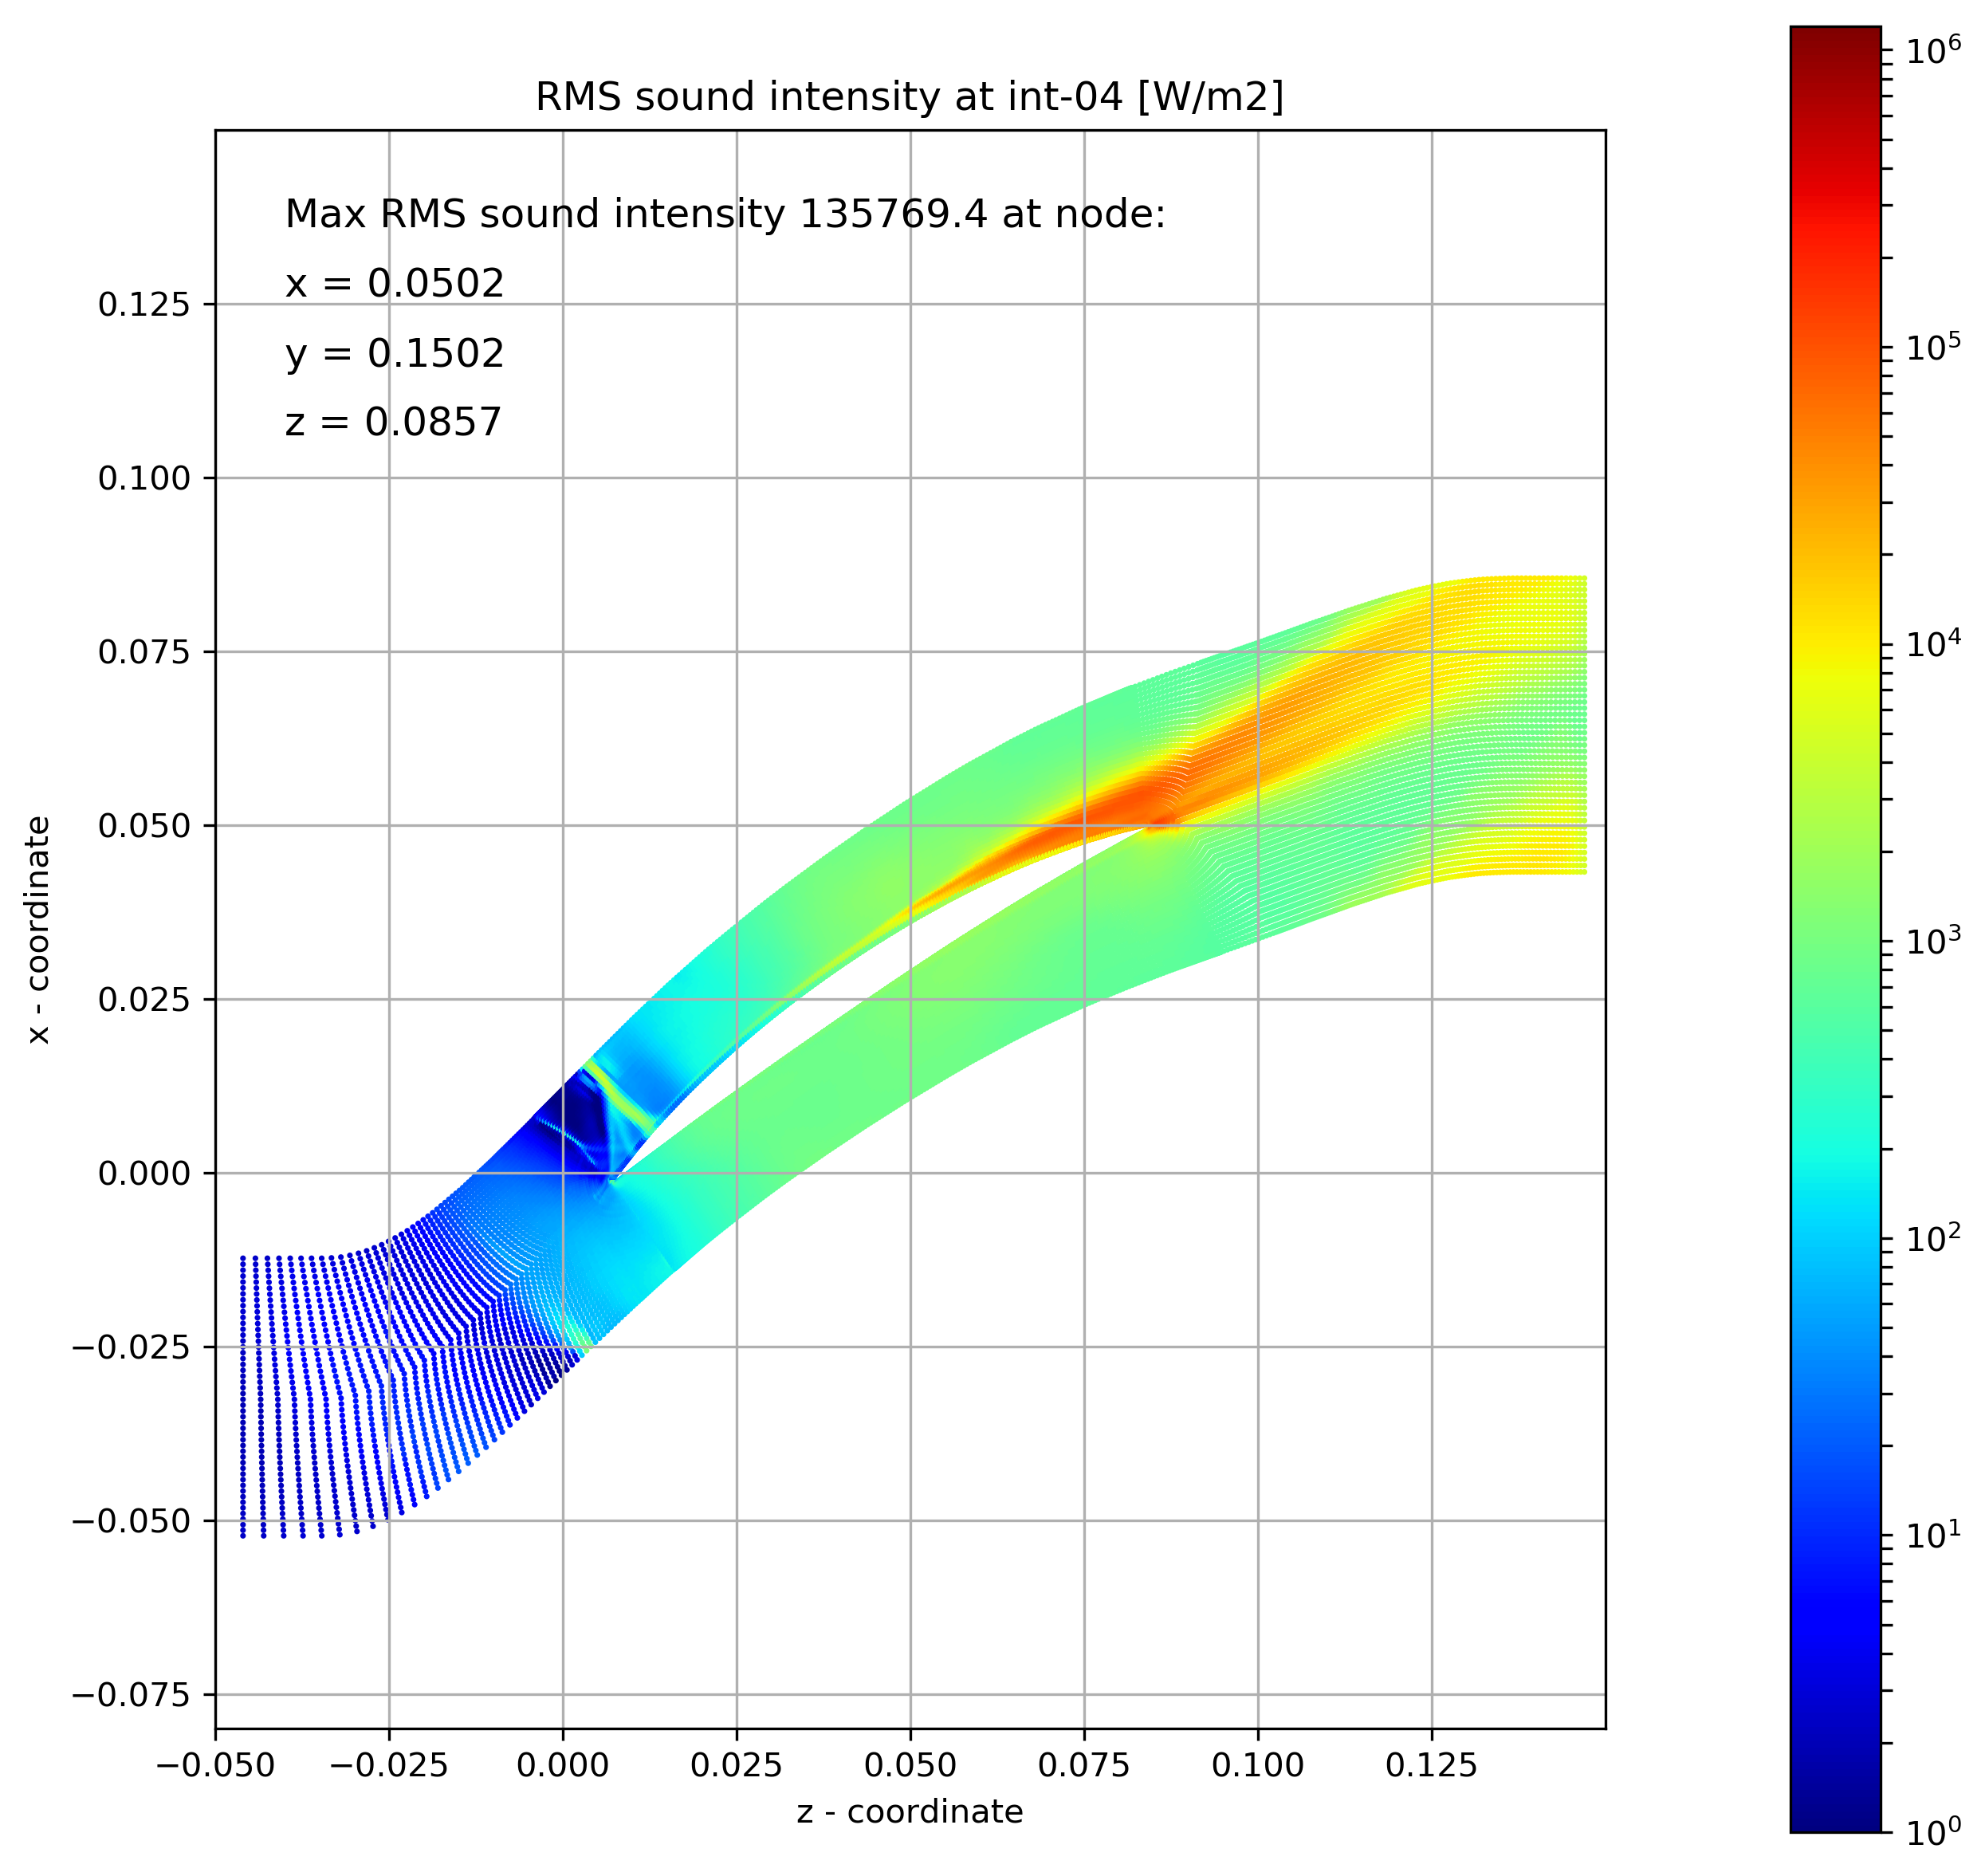
\includegraphics[width=0.75\textwidth]{Figures/int-04-rms-sil.png} \label{int-04-rms-sil}
  \caption{RMS Sound intensity at int-04 mark}
  
  \vspace*{\floatsep}% https://tex.stackexchange.com/q/26521/5764

  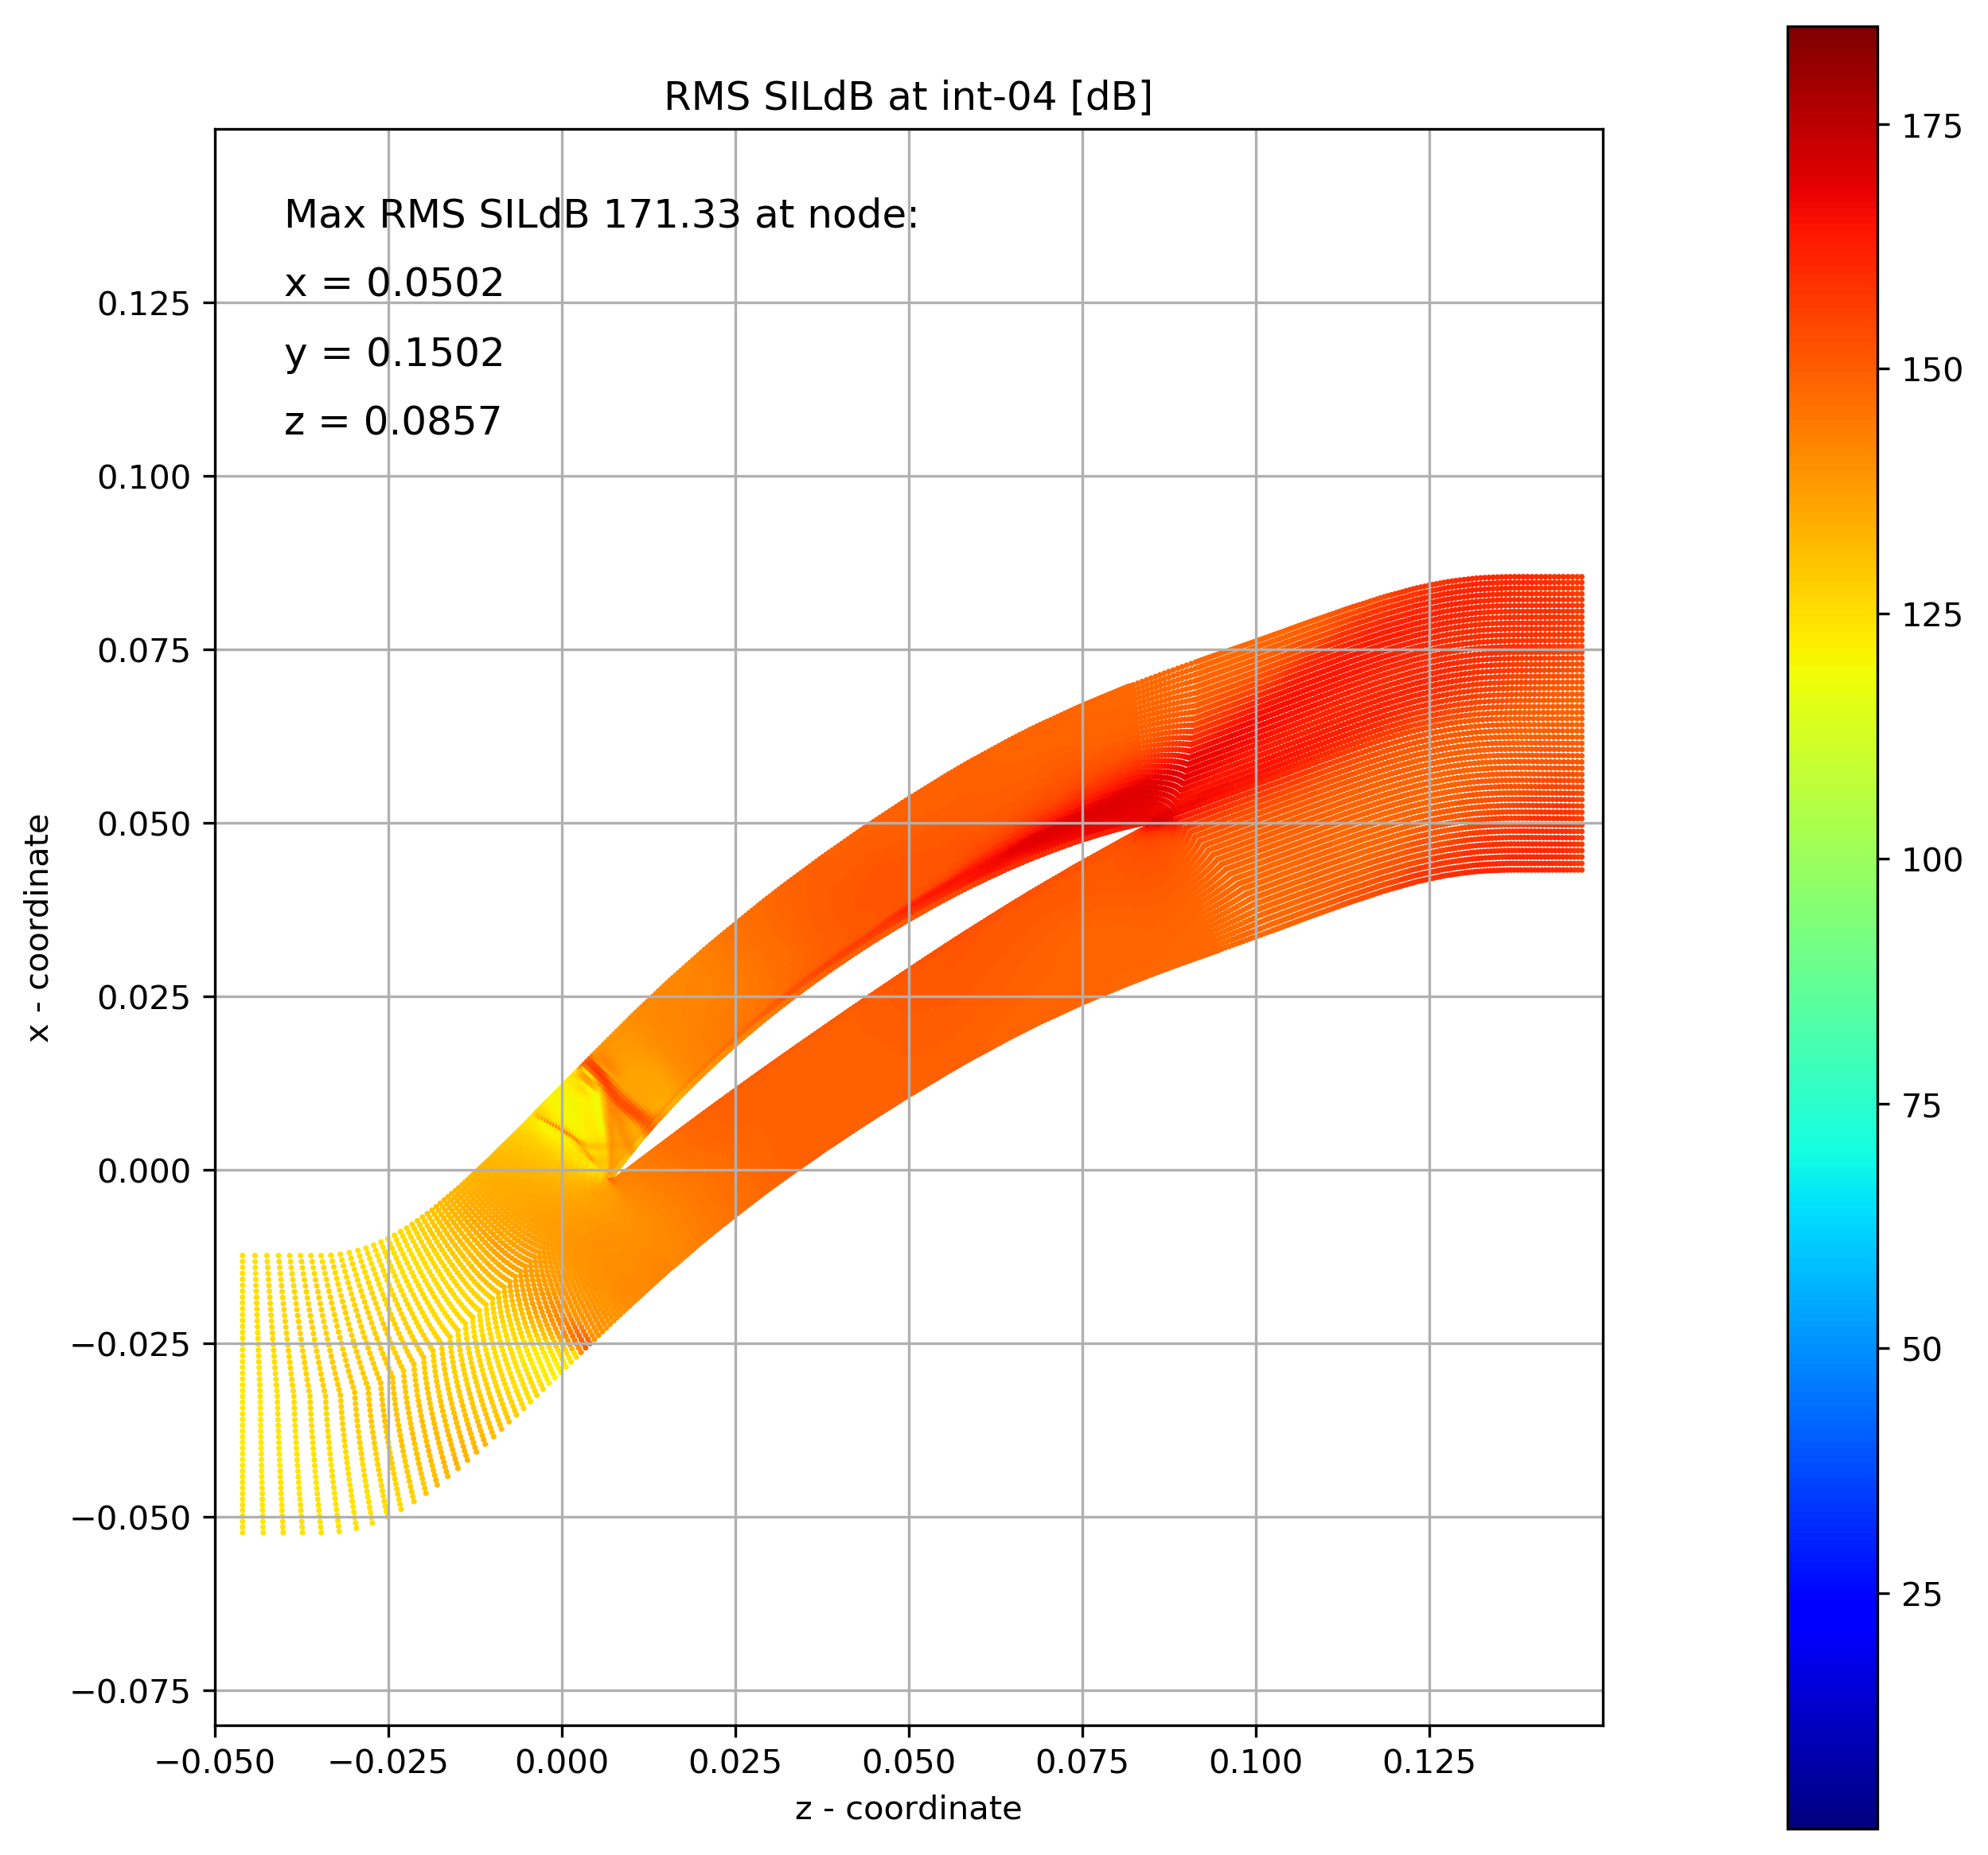
\includegraphics[width=0.75\textwidth]{Figures/int-04-rms-sildb.png} \label{int-04-rms-sildb}
  \caption{RMS Sound intensity decibel level at int-04 mark}
\end{figure}

%int-05
\begin{figure}[ht]
  \centering
  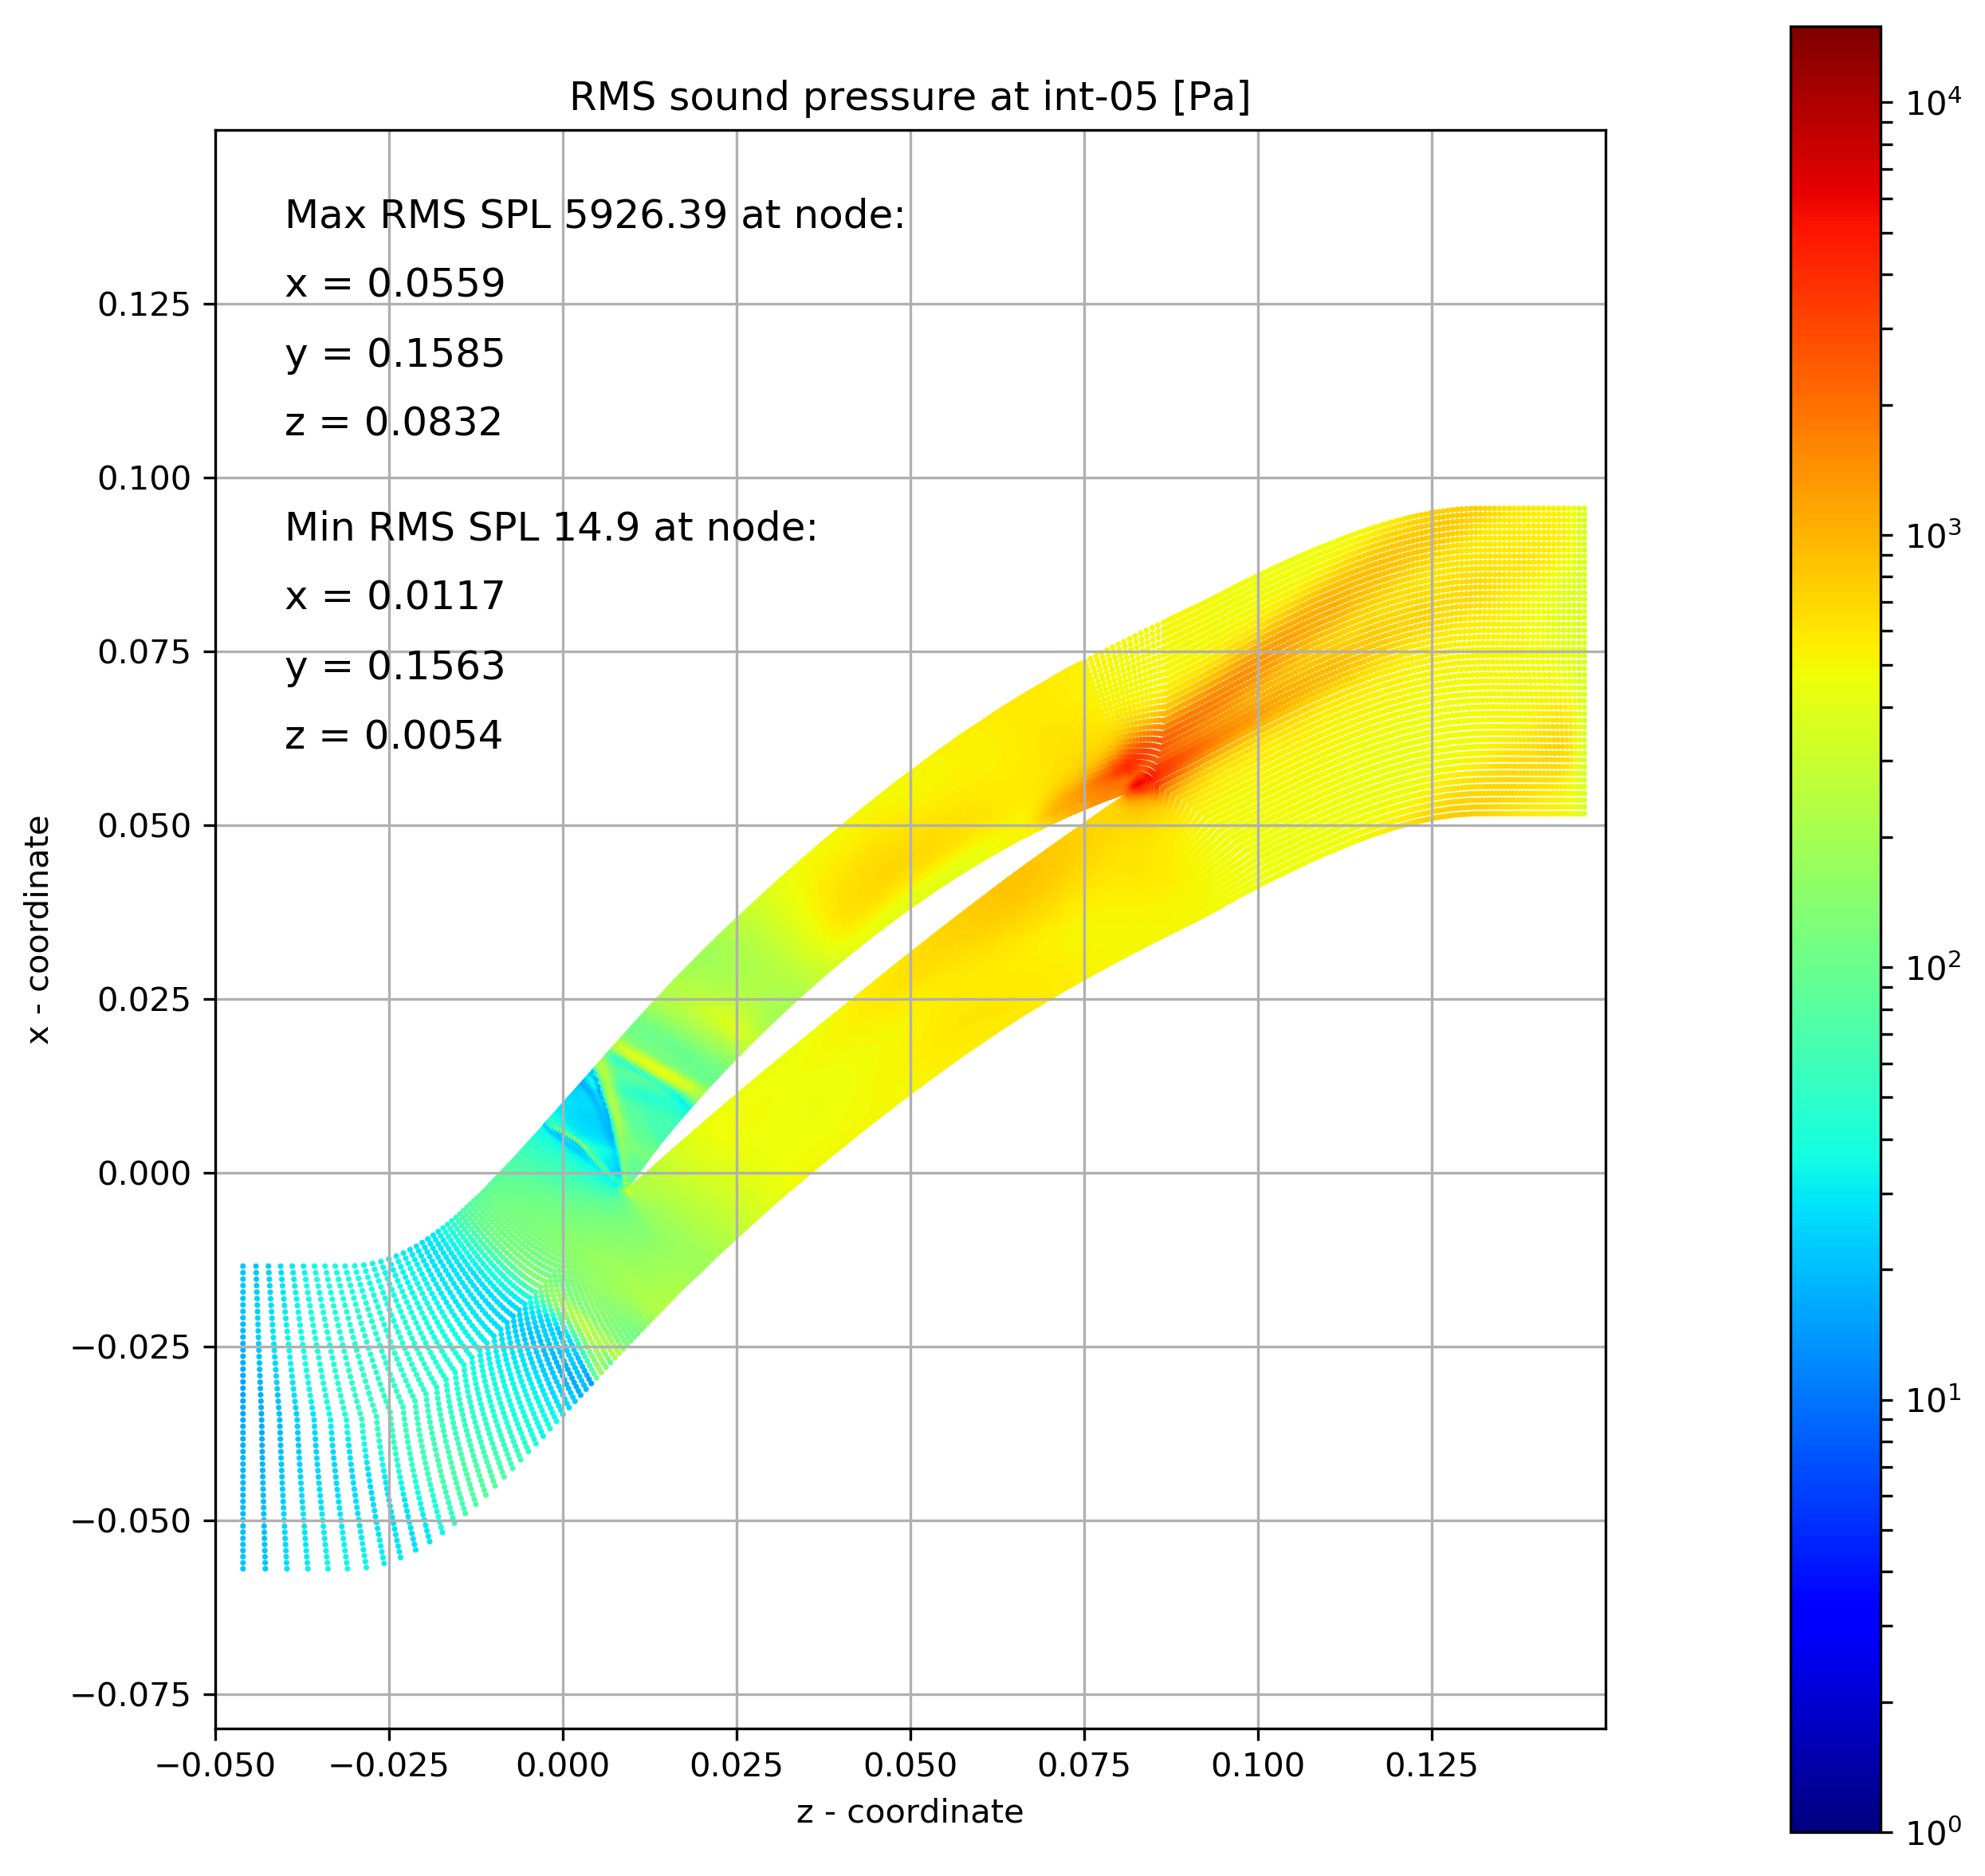
\includegraphics[width=0.75\textwidth]{Figures/int-05-rms-spl.png} \label{int-05-rms-spl}
  \caption{RMS Sound pressure at int-05 mark}
  
  \vspace*{\floatsep}% https://tex.stackexchange.com/q/26521/5764

  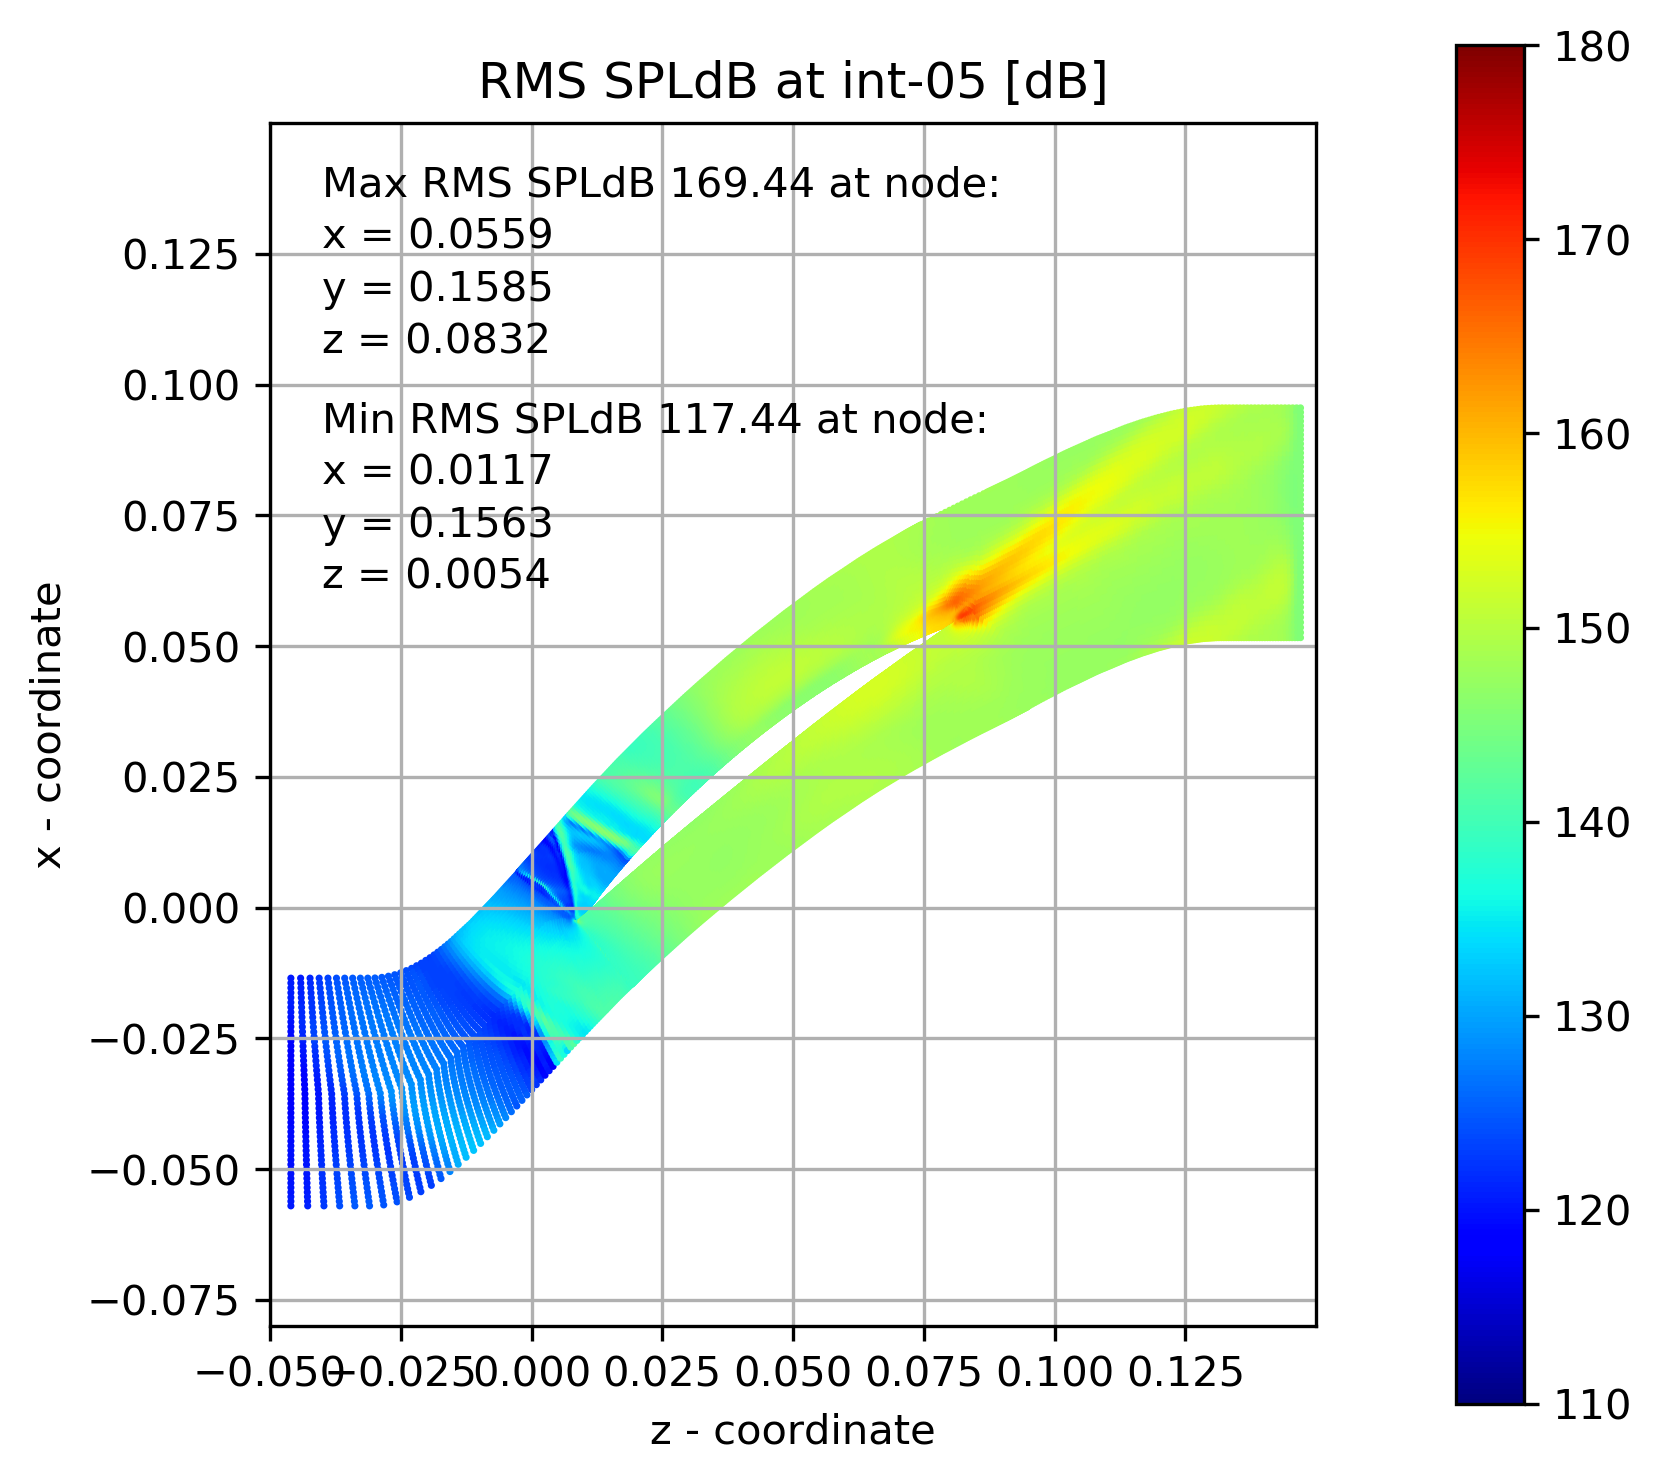
\includegraphics[width=0.75\textwidth]{Figures/int-05-rms-spldb.png} \label{int-05-rms-spldb}
  \caption{RMS Sound pressure decibel level at int-05 mark}
\end{figure}
%int-05
\begin{figure}[ht]
  \centering
  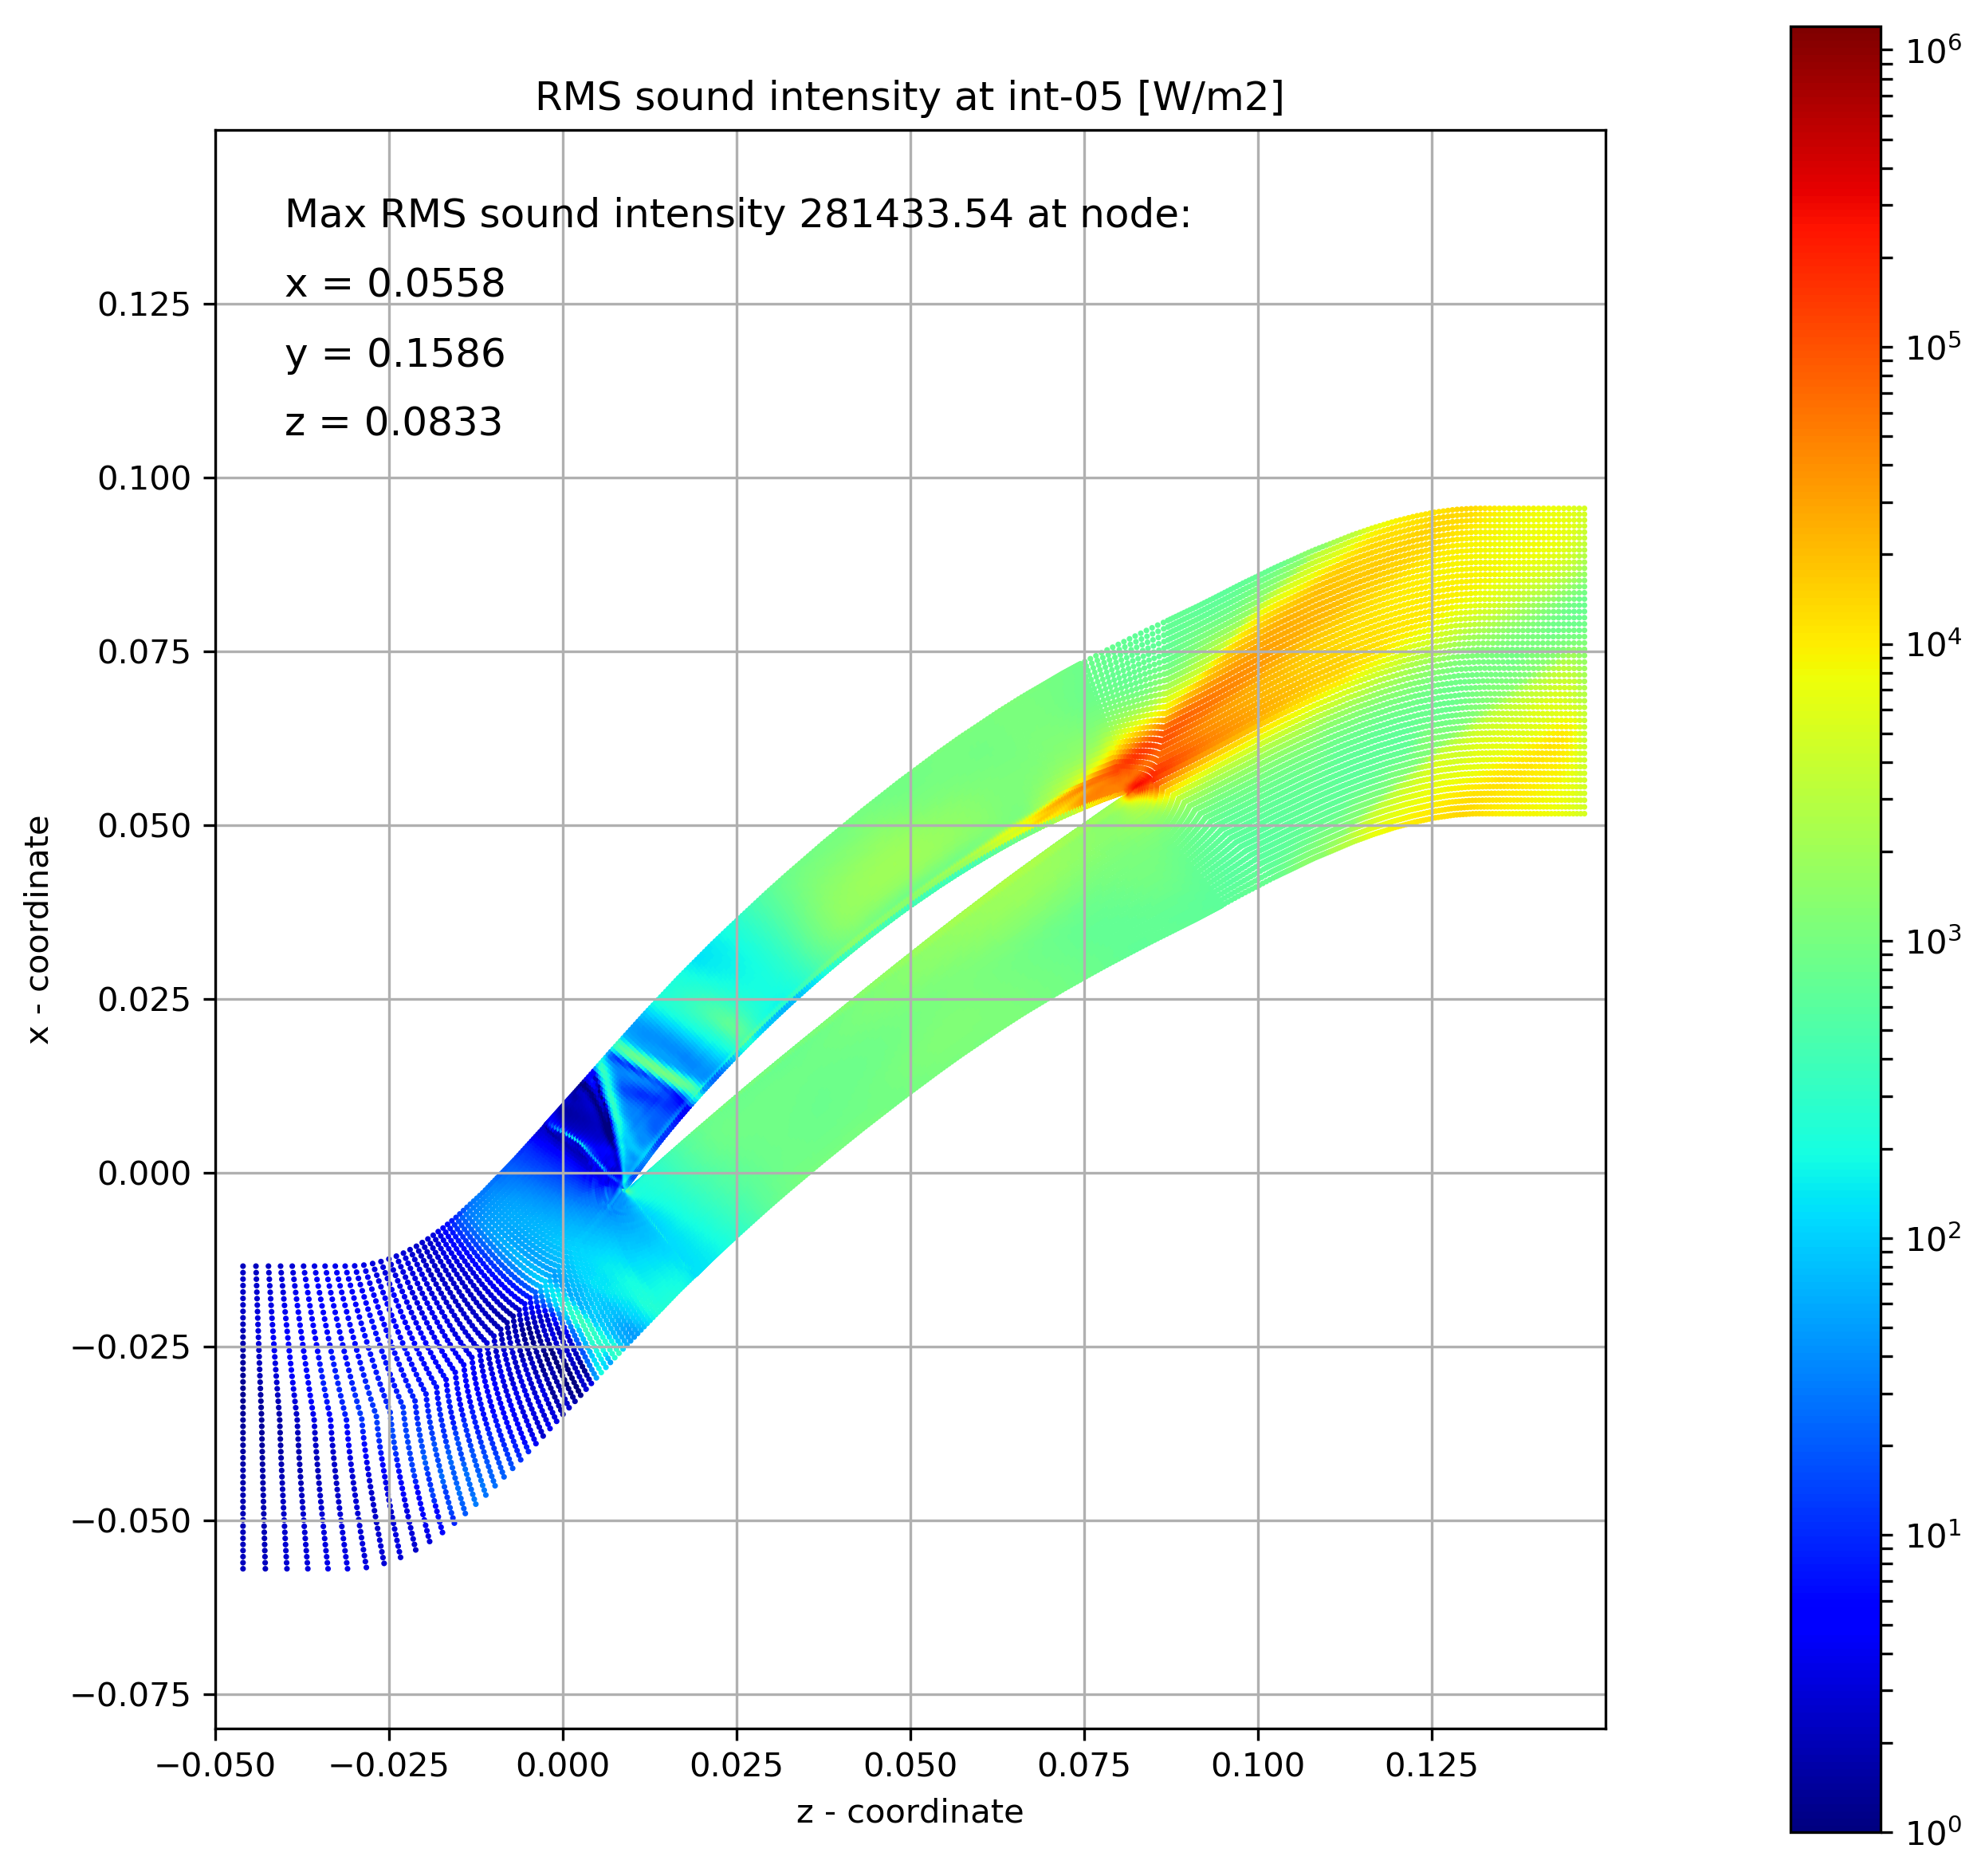
\includegraphics[width=0.75\textwidth]{Figures/int-05-rms-sil.png} \label{int-05-rms-sil}
  \caption{RMS Sound intensity at int-05 mark}
  
  \vspace*{\floatsep}% https://tex.stackexchange.com/q/26521/5764

  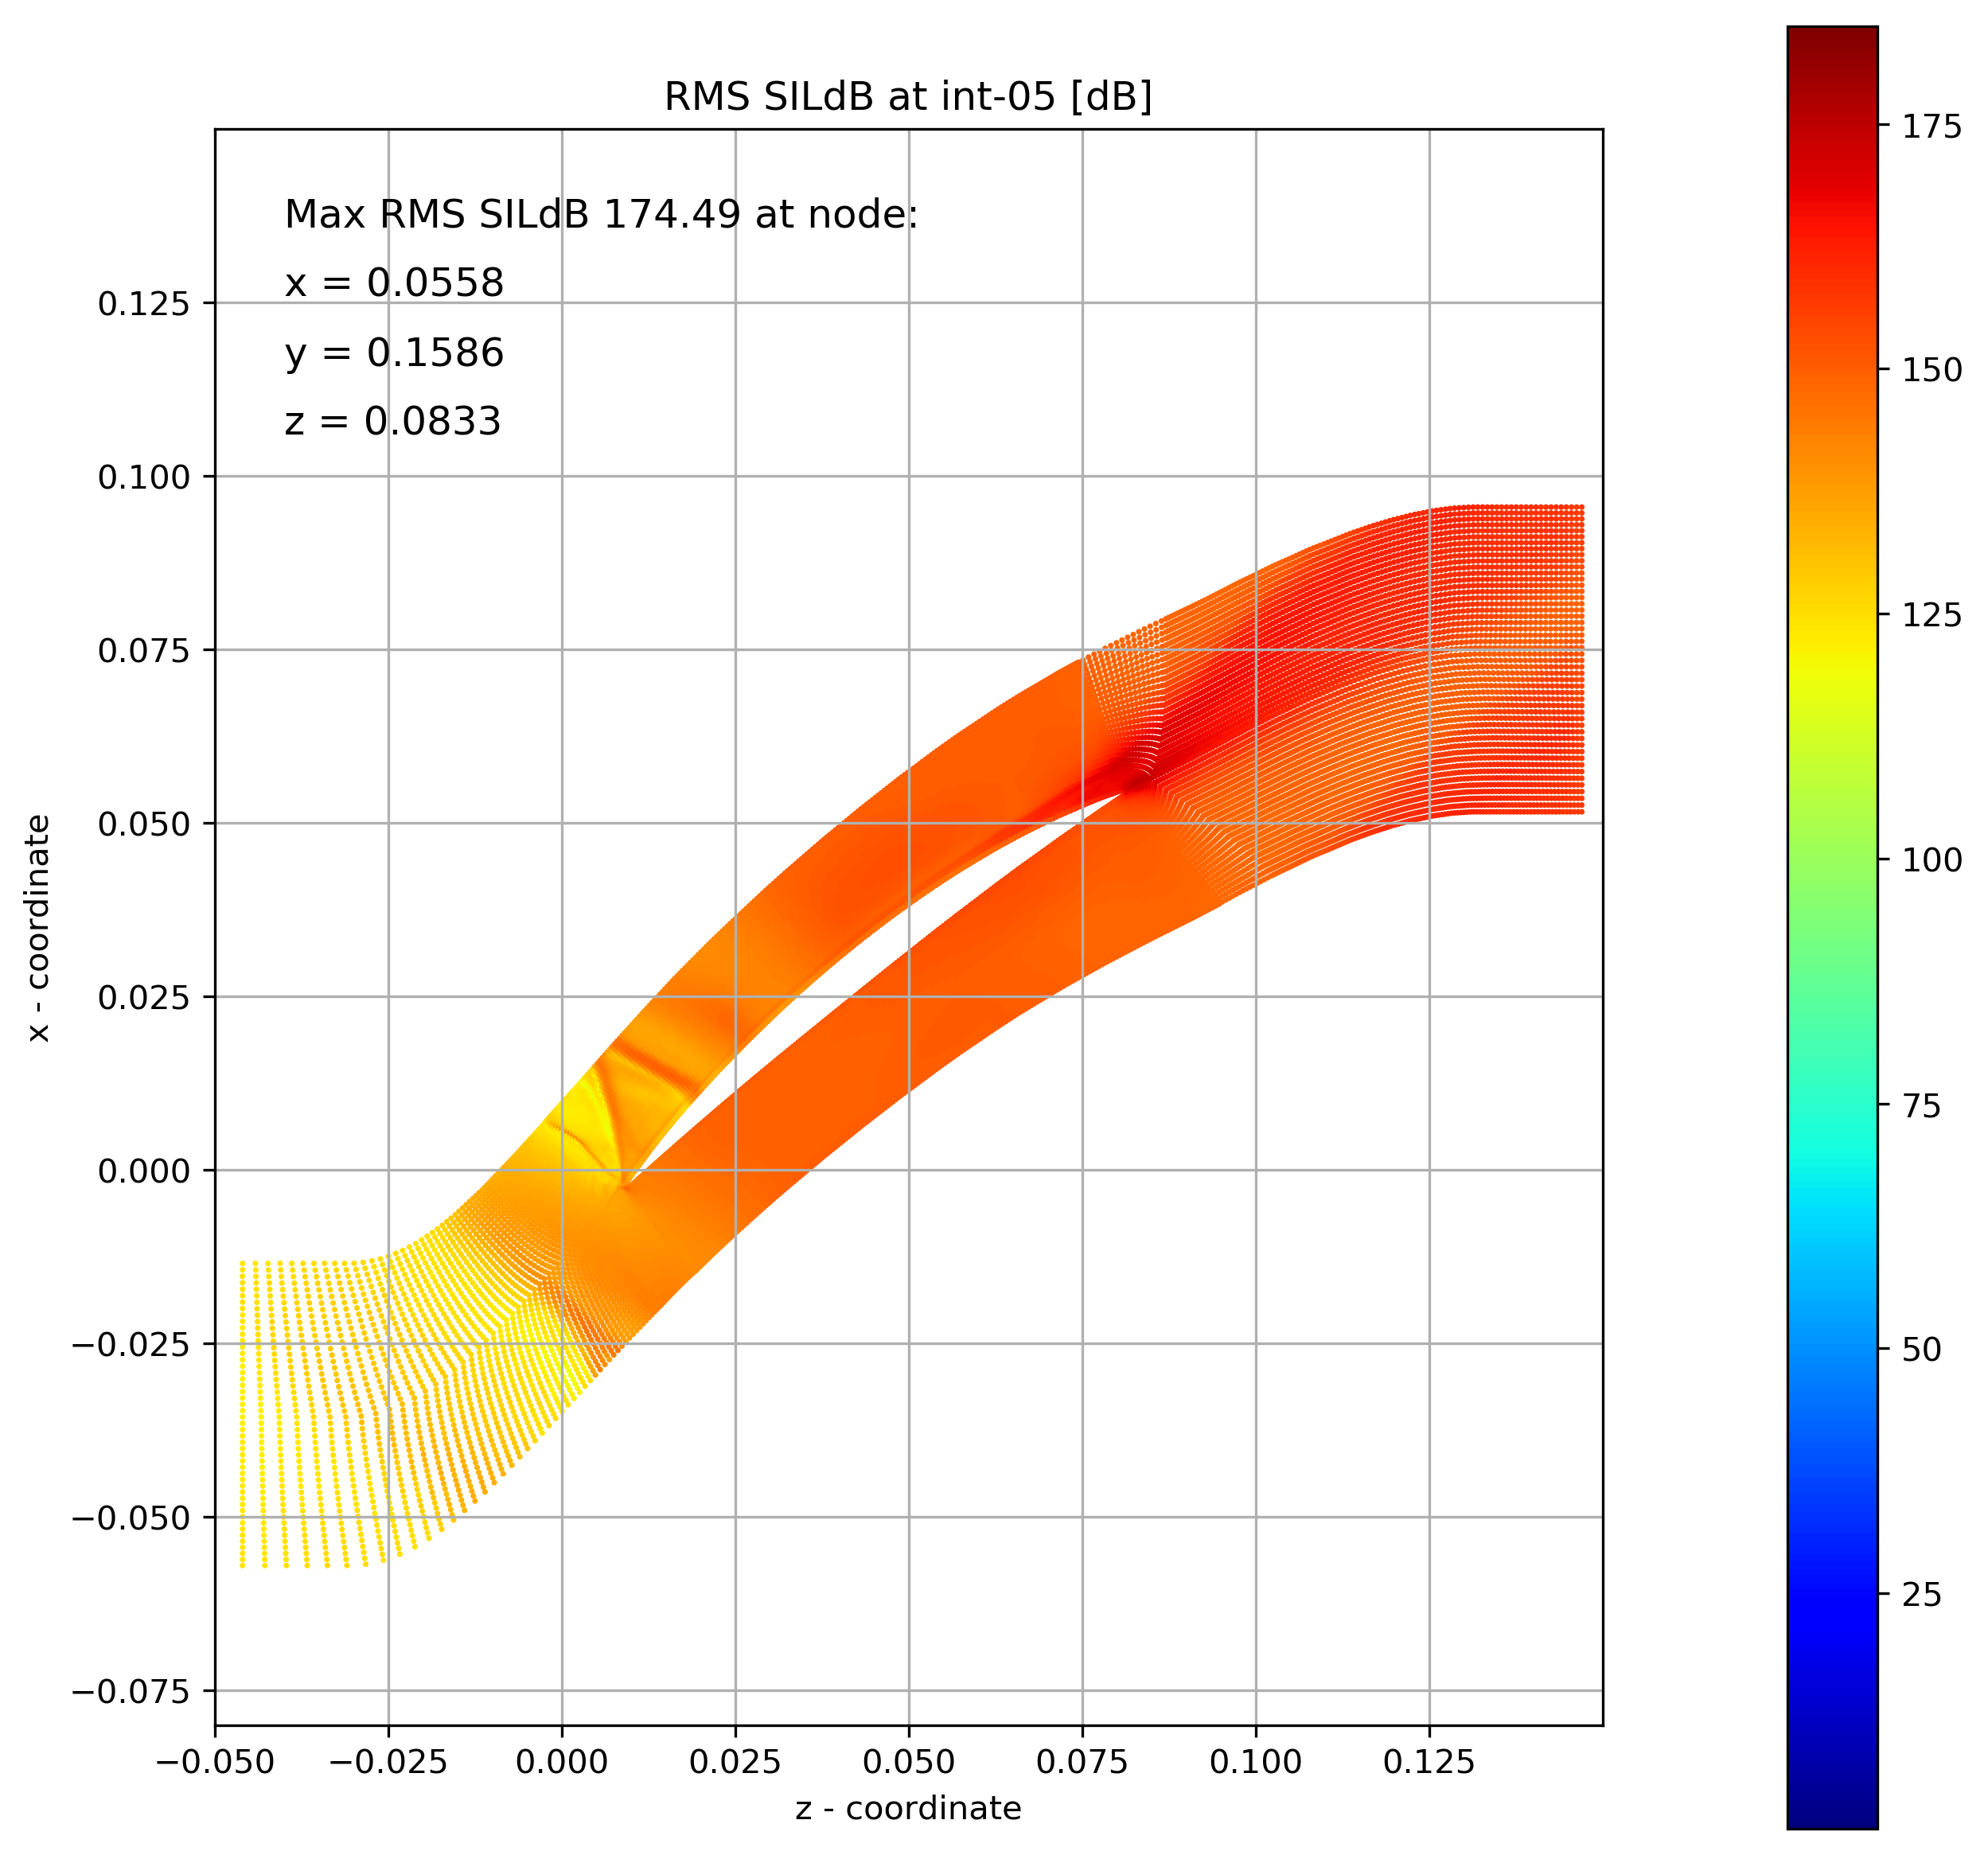
\includegraphics[width=0.75\textwidth]{Figures/int-05-rms-sildb.png} \label{int-05-rms-sildb}
  \caption{RMS Sound intensity decibel level at int-05 mark}
\end{figure}


%int-06
\begin{figure}[ht]
  \centering
  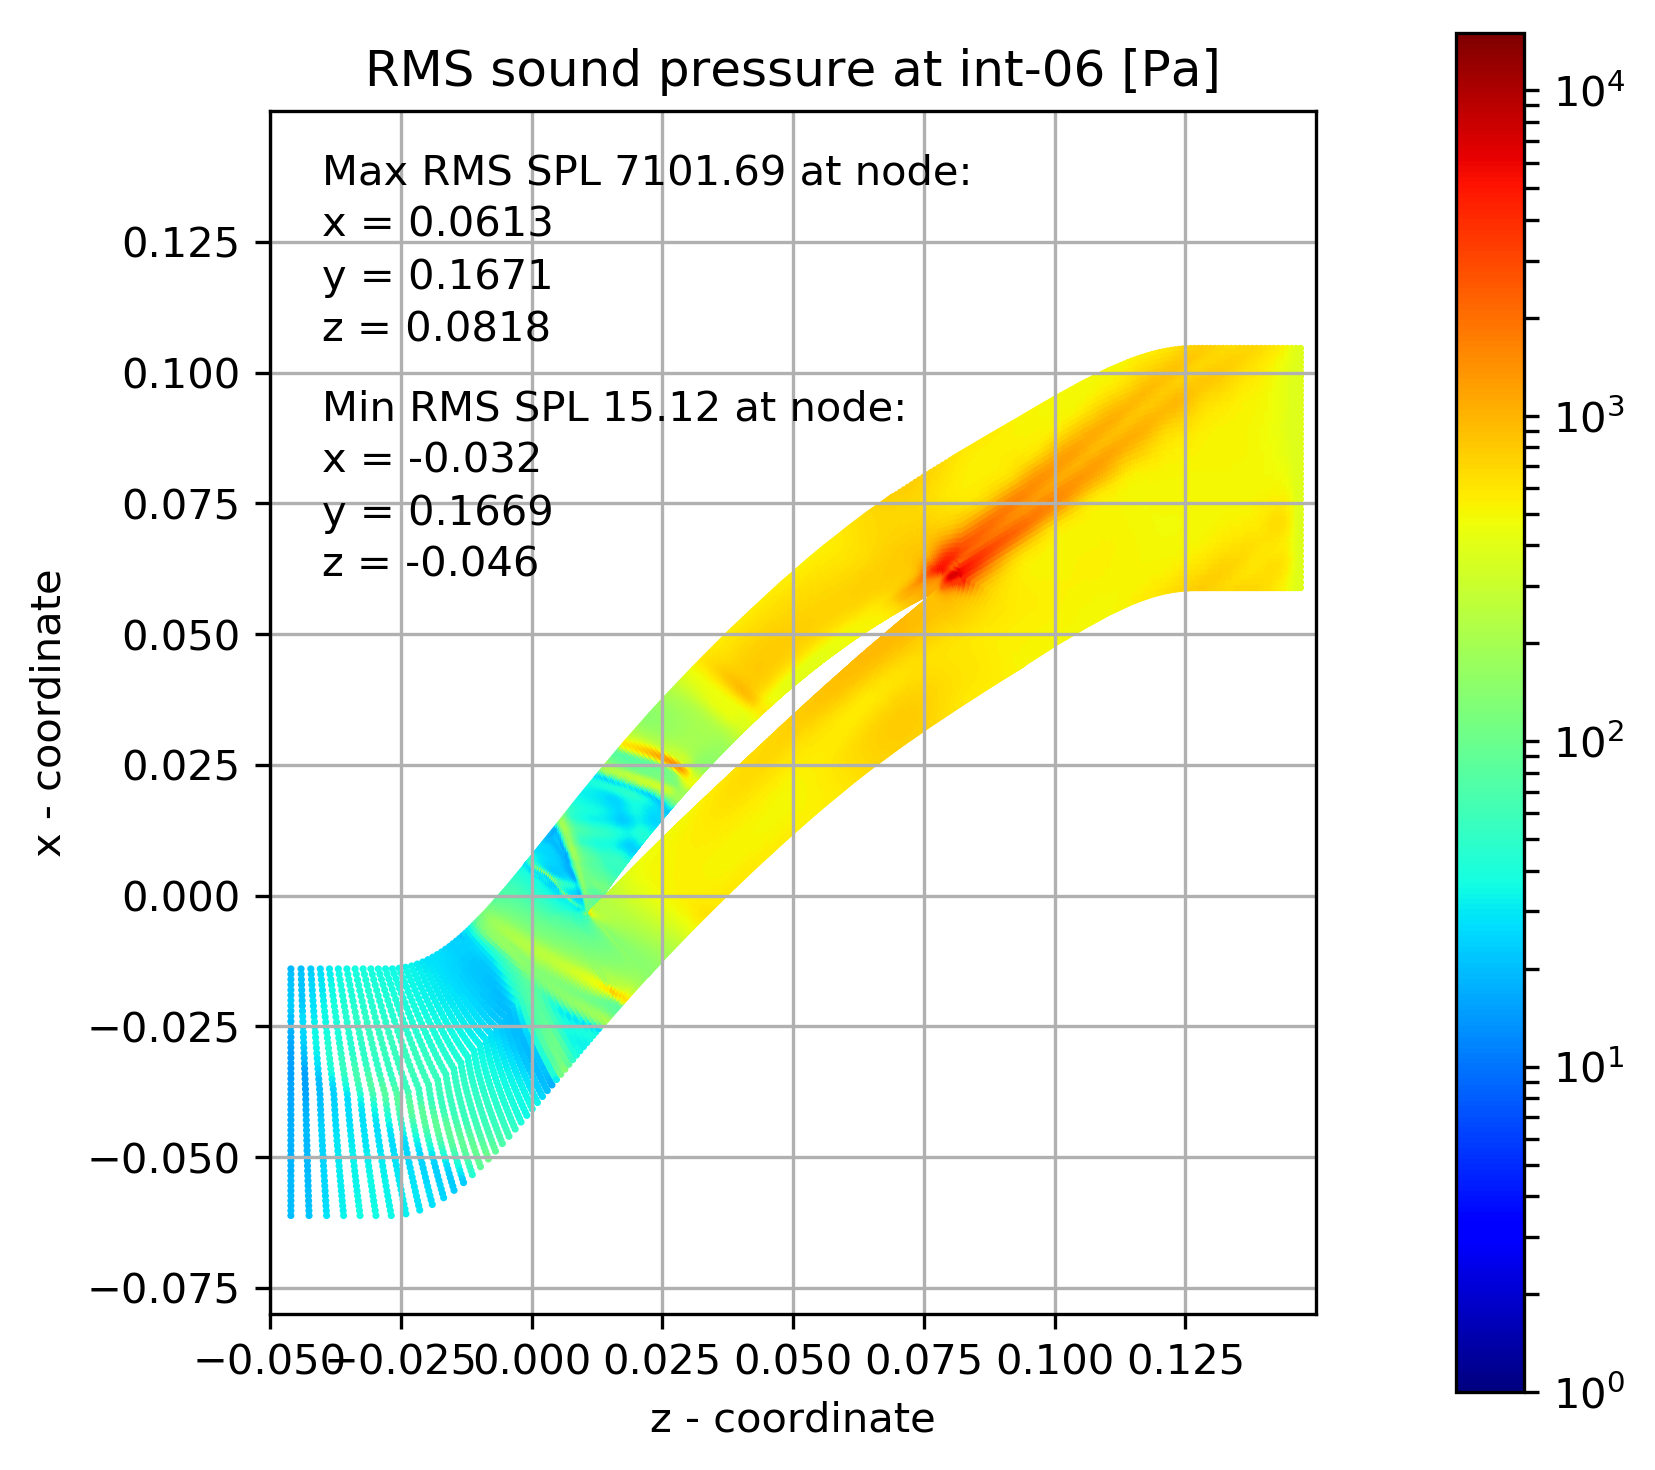
\includegraphics[width=0.75\textwidth]{Figures/int-06-rms-spl.png} \label{int-06-rms-spl}
  \caption{RMS Sound pressure at int-06 mark}
  
  \vspace*{\floatsep}% https://tex.stackexchange.com/q/26521/5764

  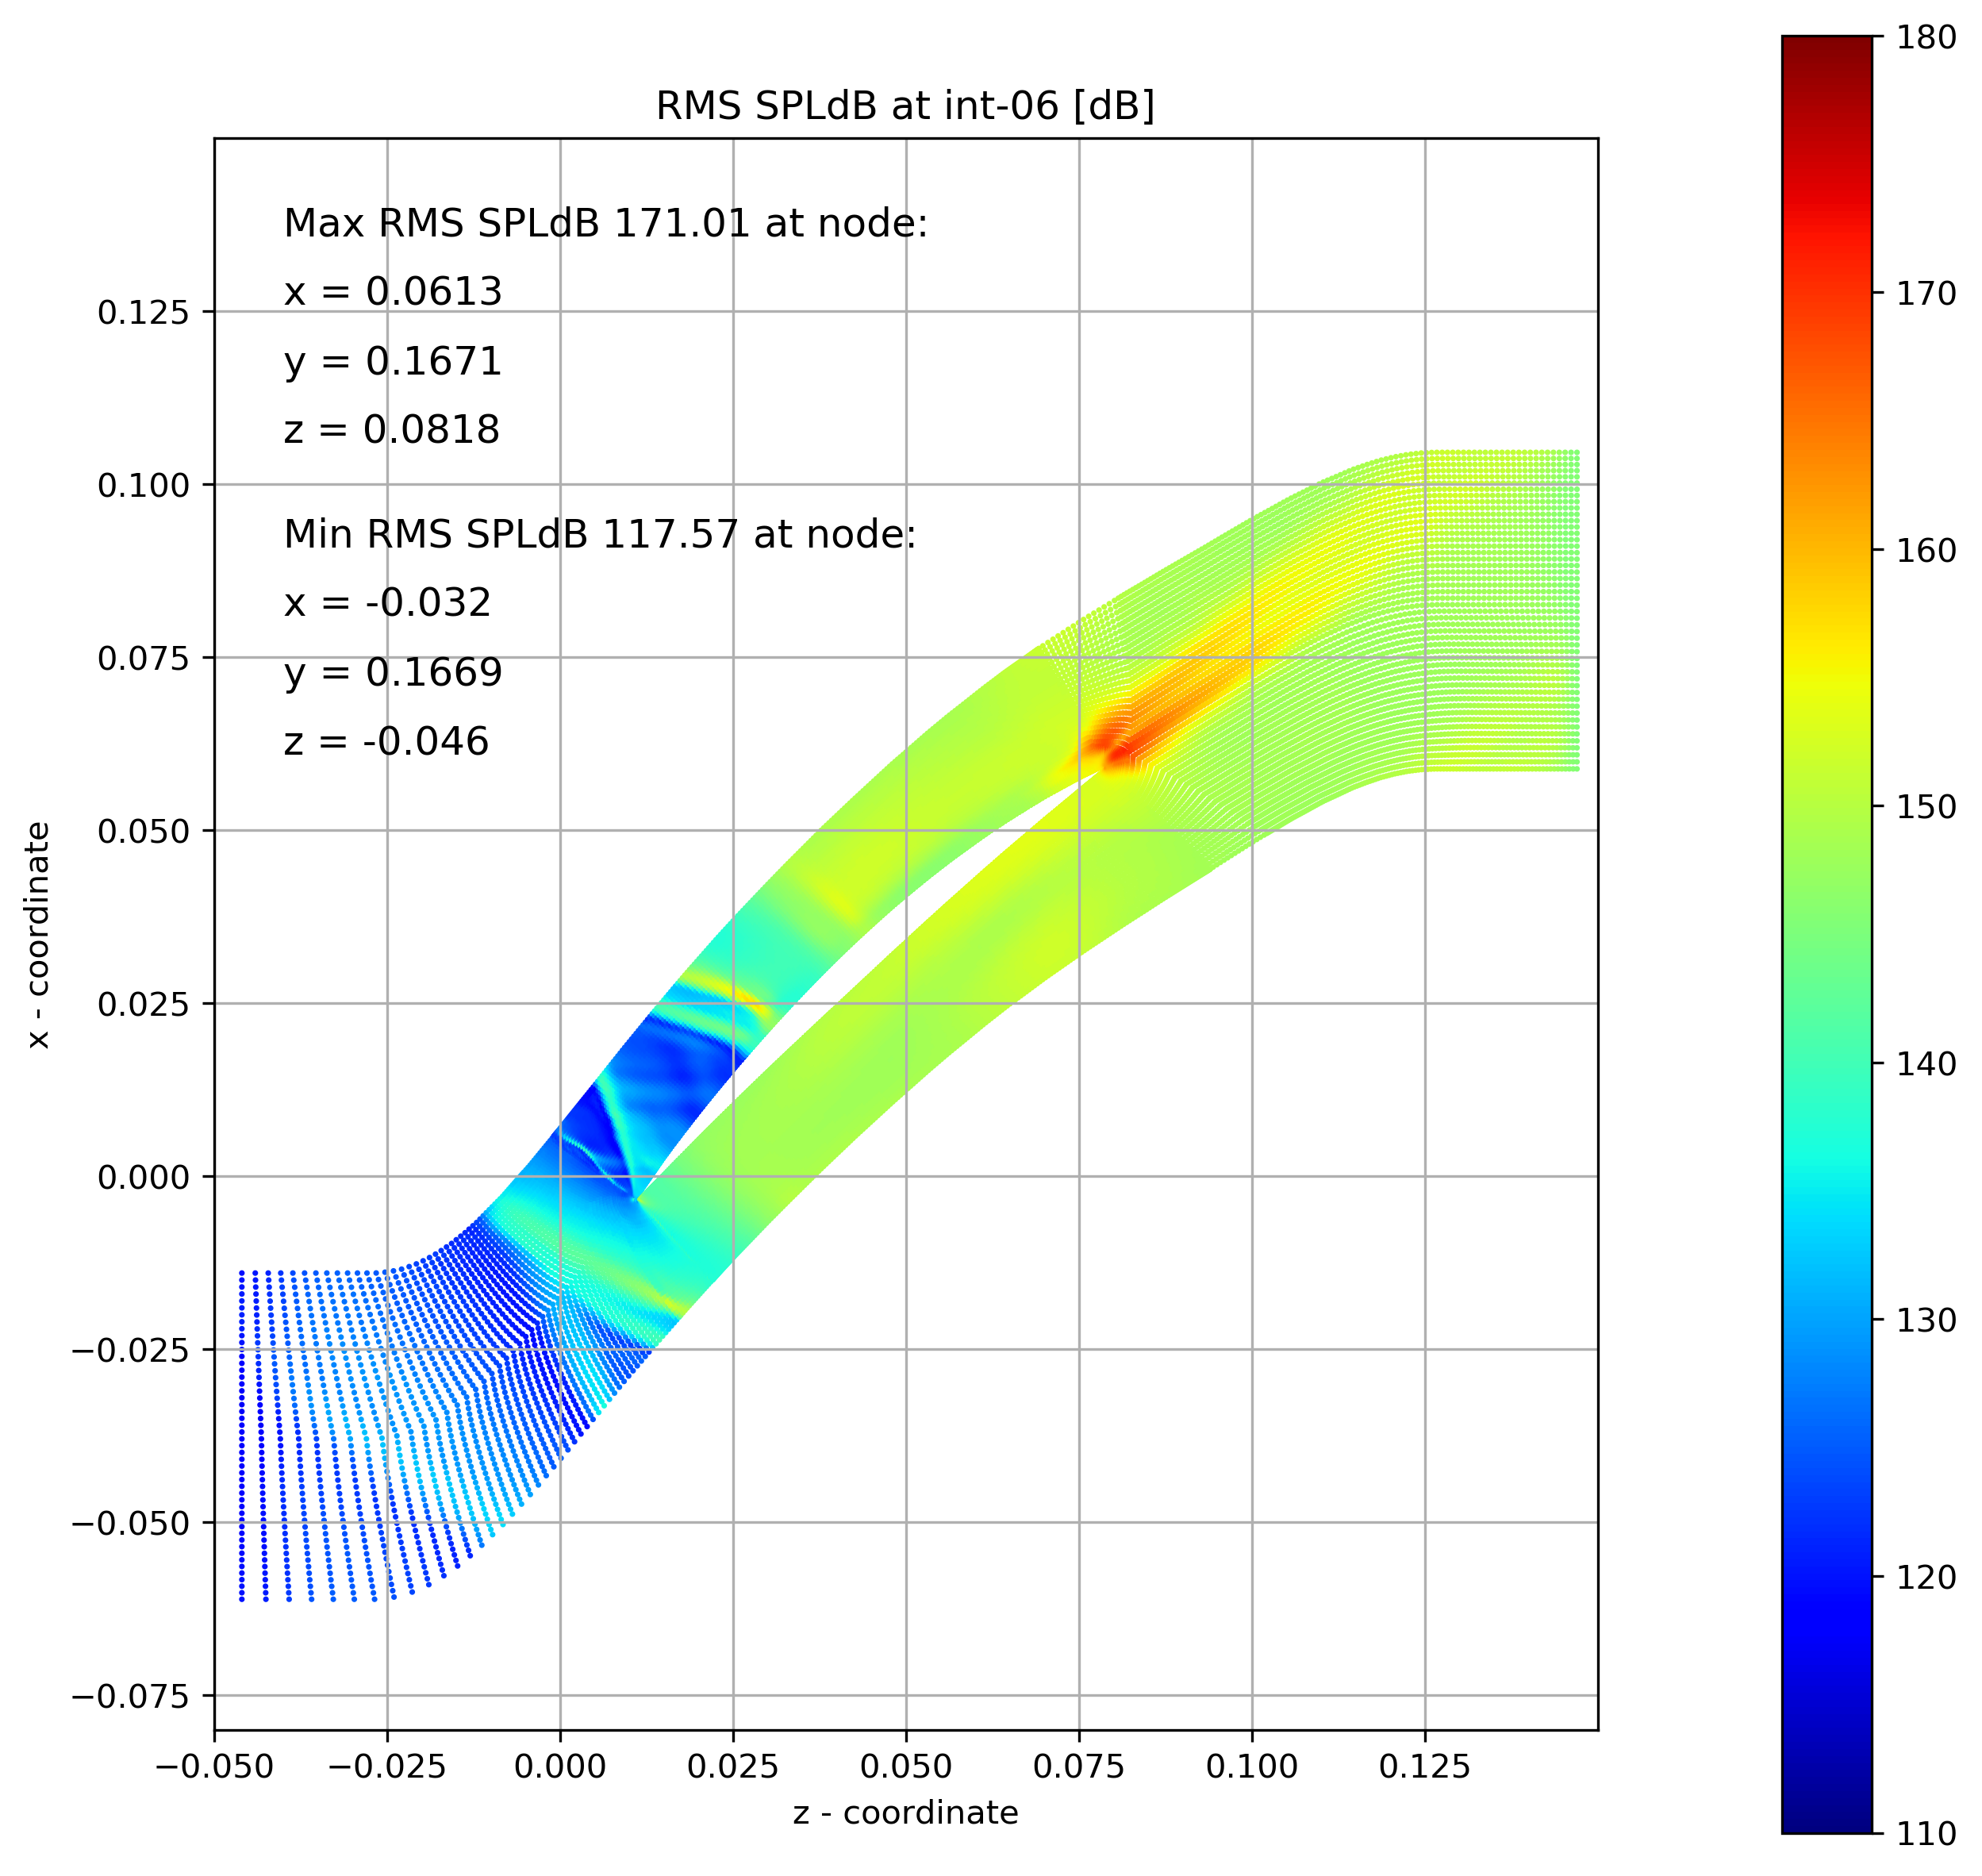
\includegraphics[width=0.75\textwidth]{Figures/int-06-rms-spldb.png} \label{int-06-rms-spldb}
  \caption{RMS Sound pressure decibel level at int-06 mark}
\end{figure}
%int-06
\begin{figure}[ht]
  \centering
  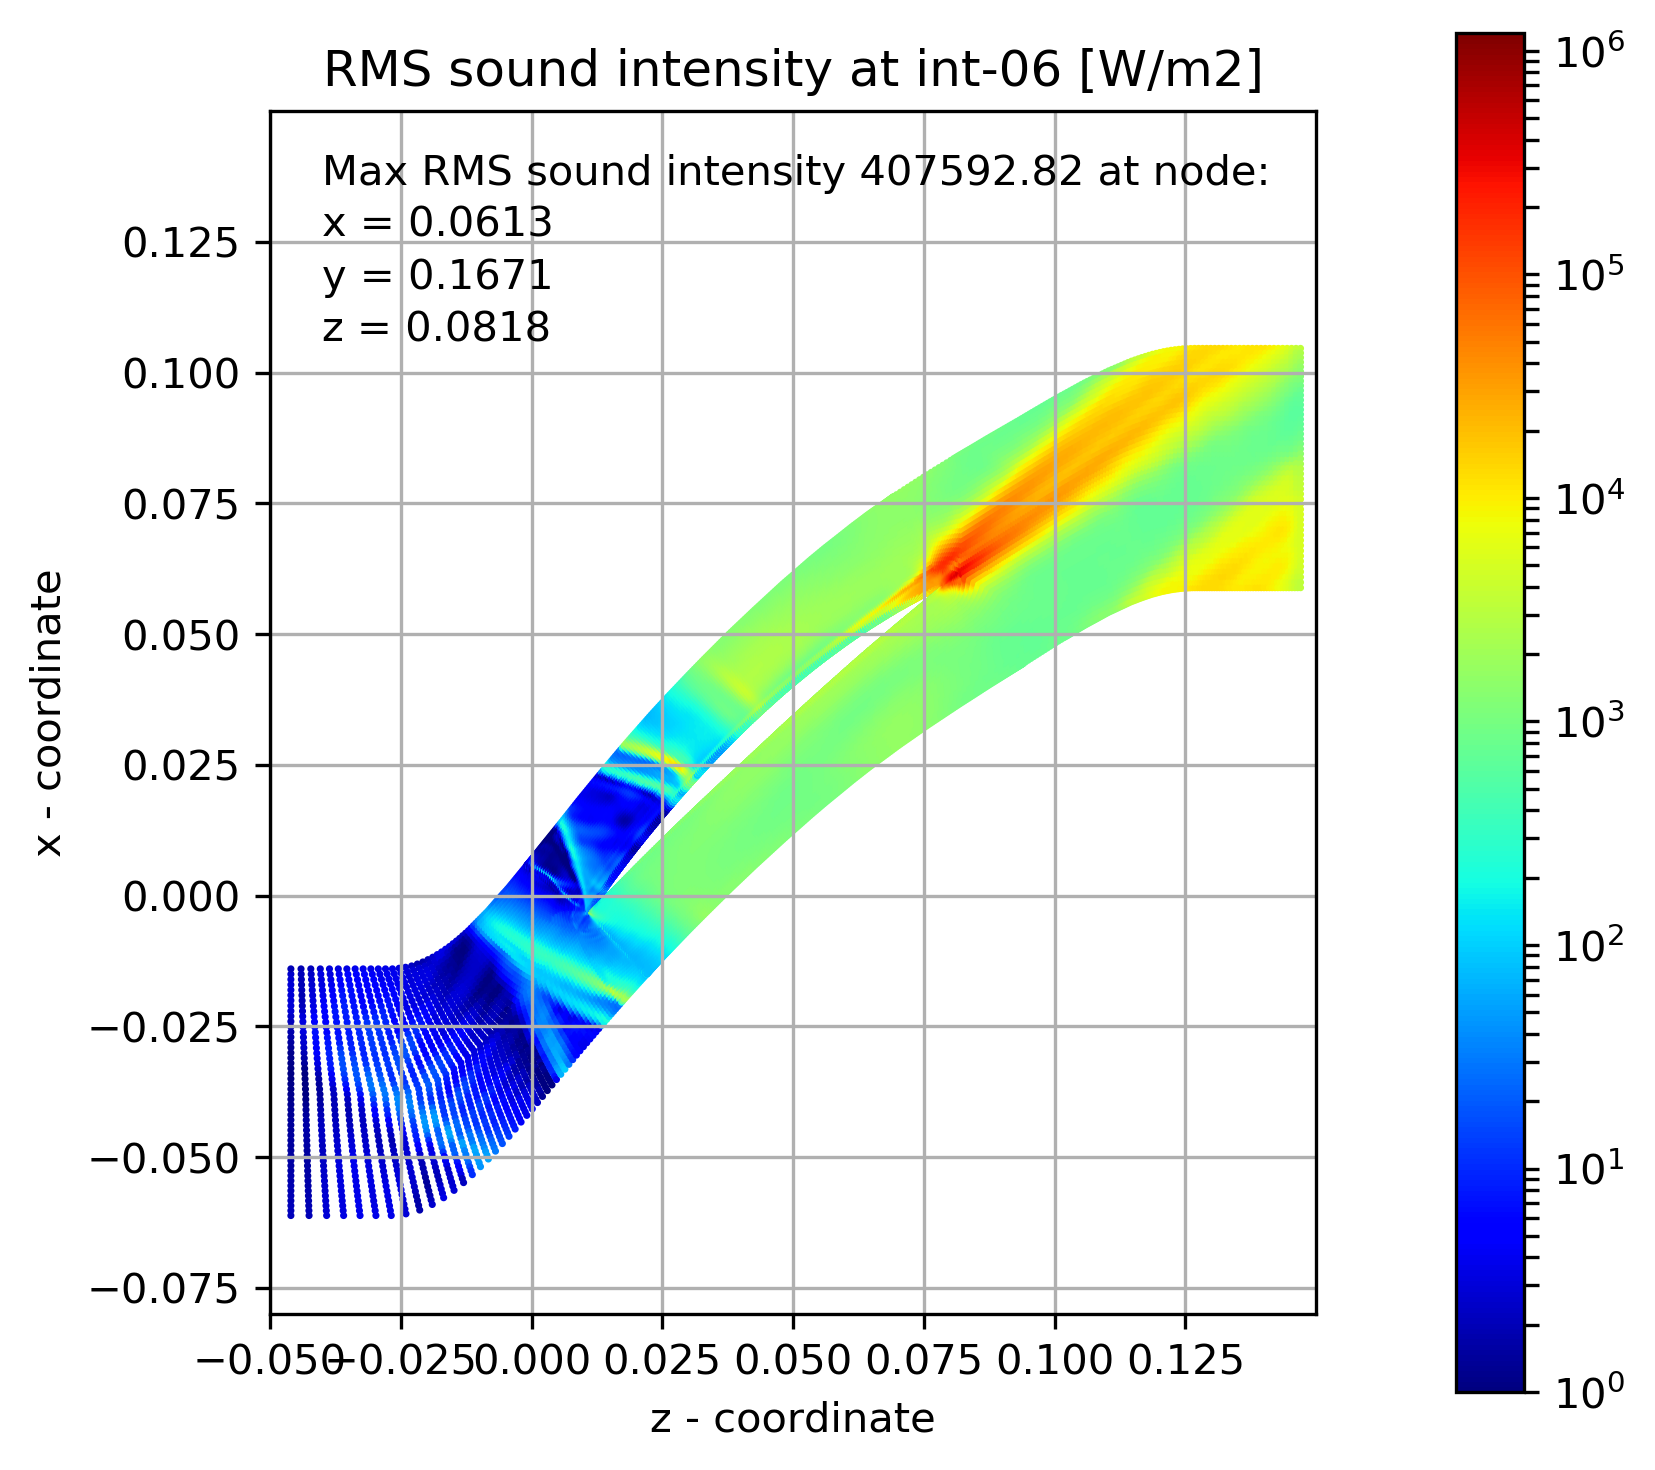
\includegraphics[width=0.75\textwidth]{Figures/int-06-rms-sil.png} \label{int-06-rms-sil}
  \caption{RMS Sound intensity at int-06 mark}
  
  \vspace*{\floatsep}% https://tex.stackexchange.com/q/26521/5764

  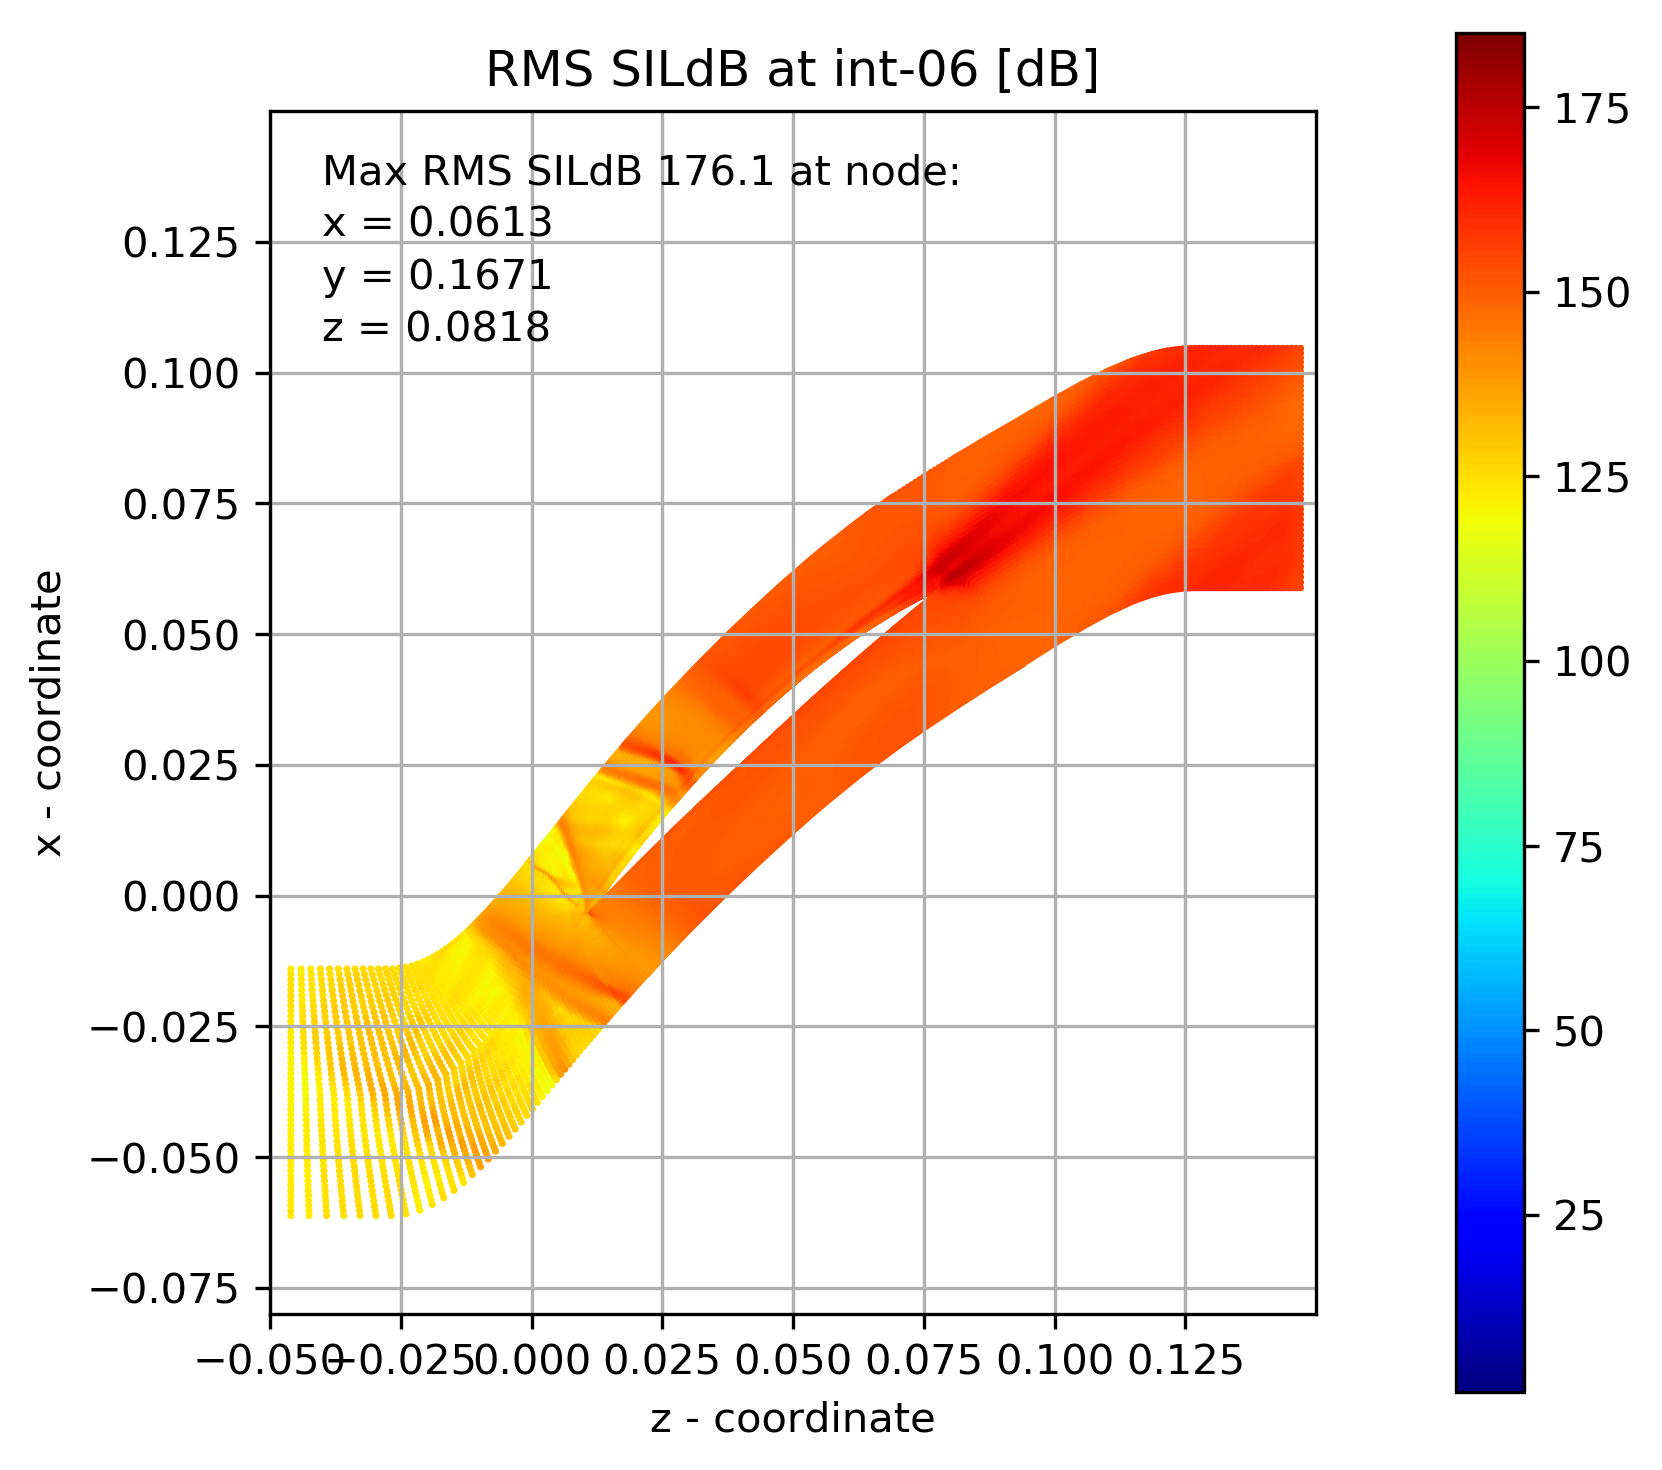
\includegraphics[width=0.75\textwidth]{Figures/int-06-rms-sildb.png} \label{int-06-rms-sildb}
  \caption{RMS Sound intensity decibel level at int-06 mark}
\end{figure}


%int-07
\begin{figure}[ht]
  \centering
  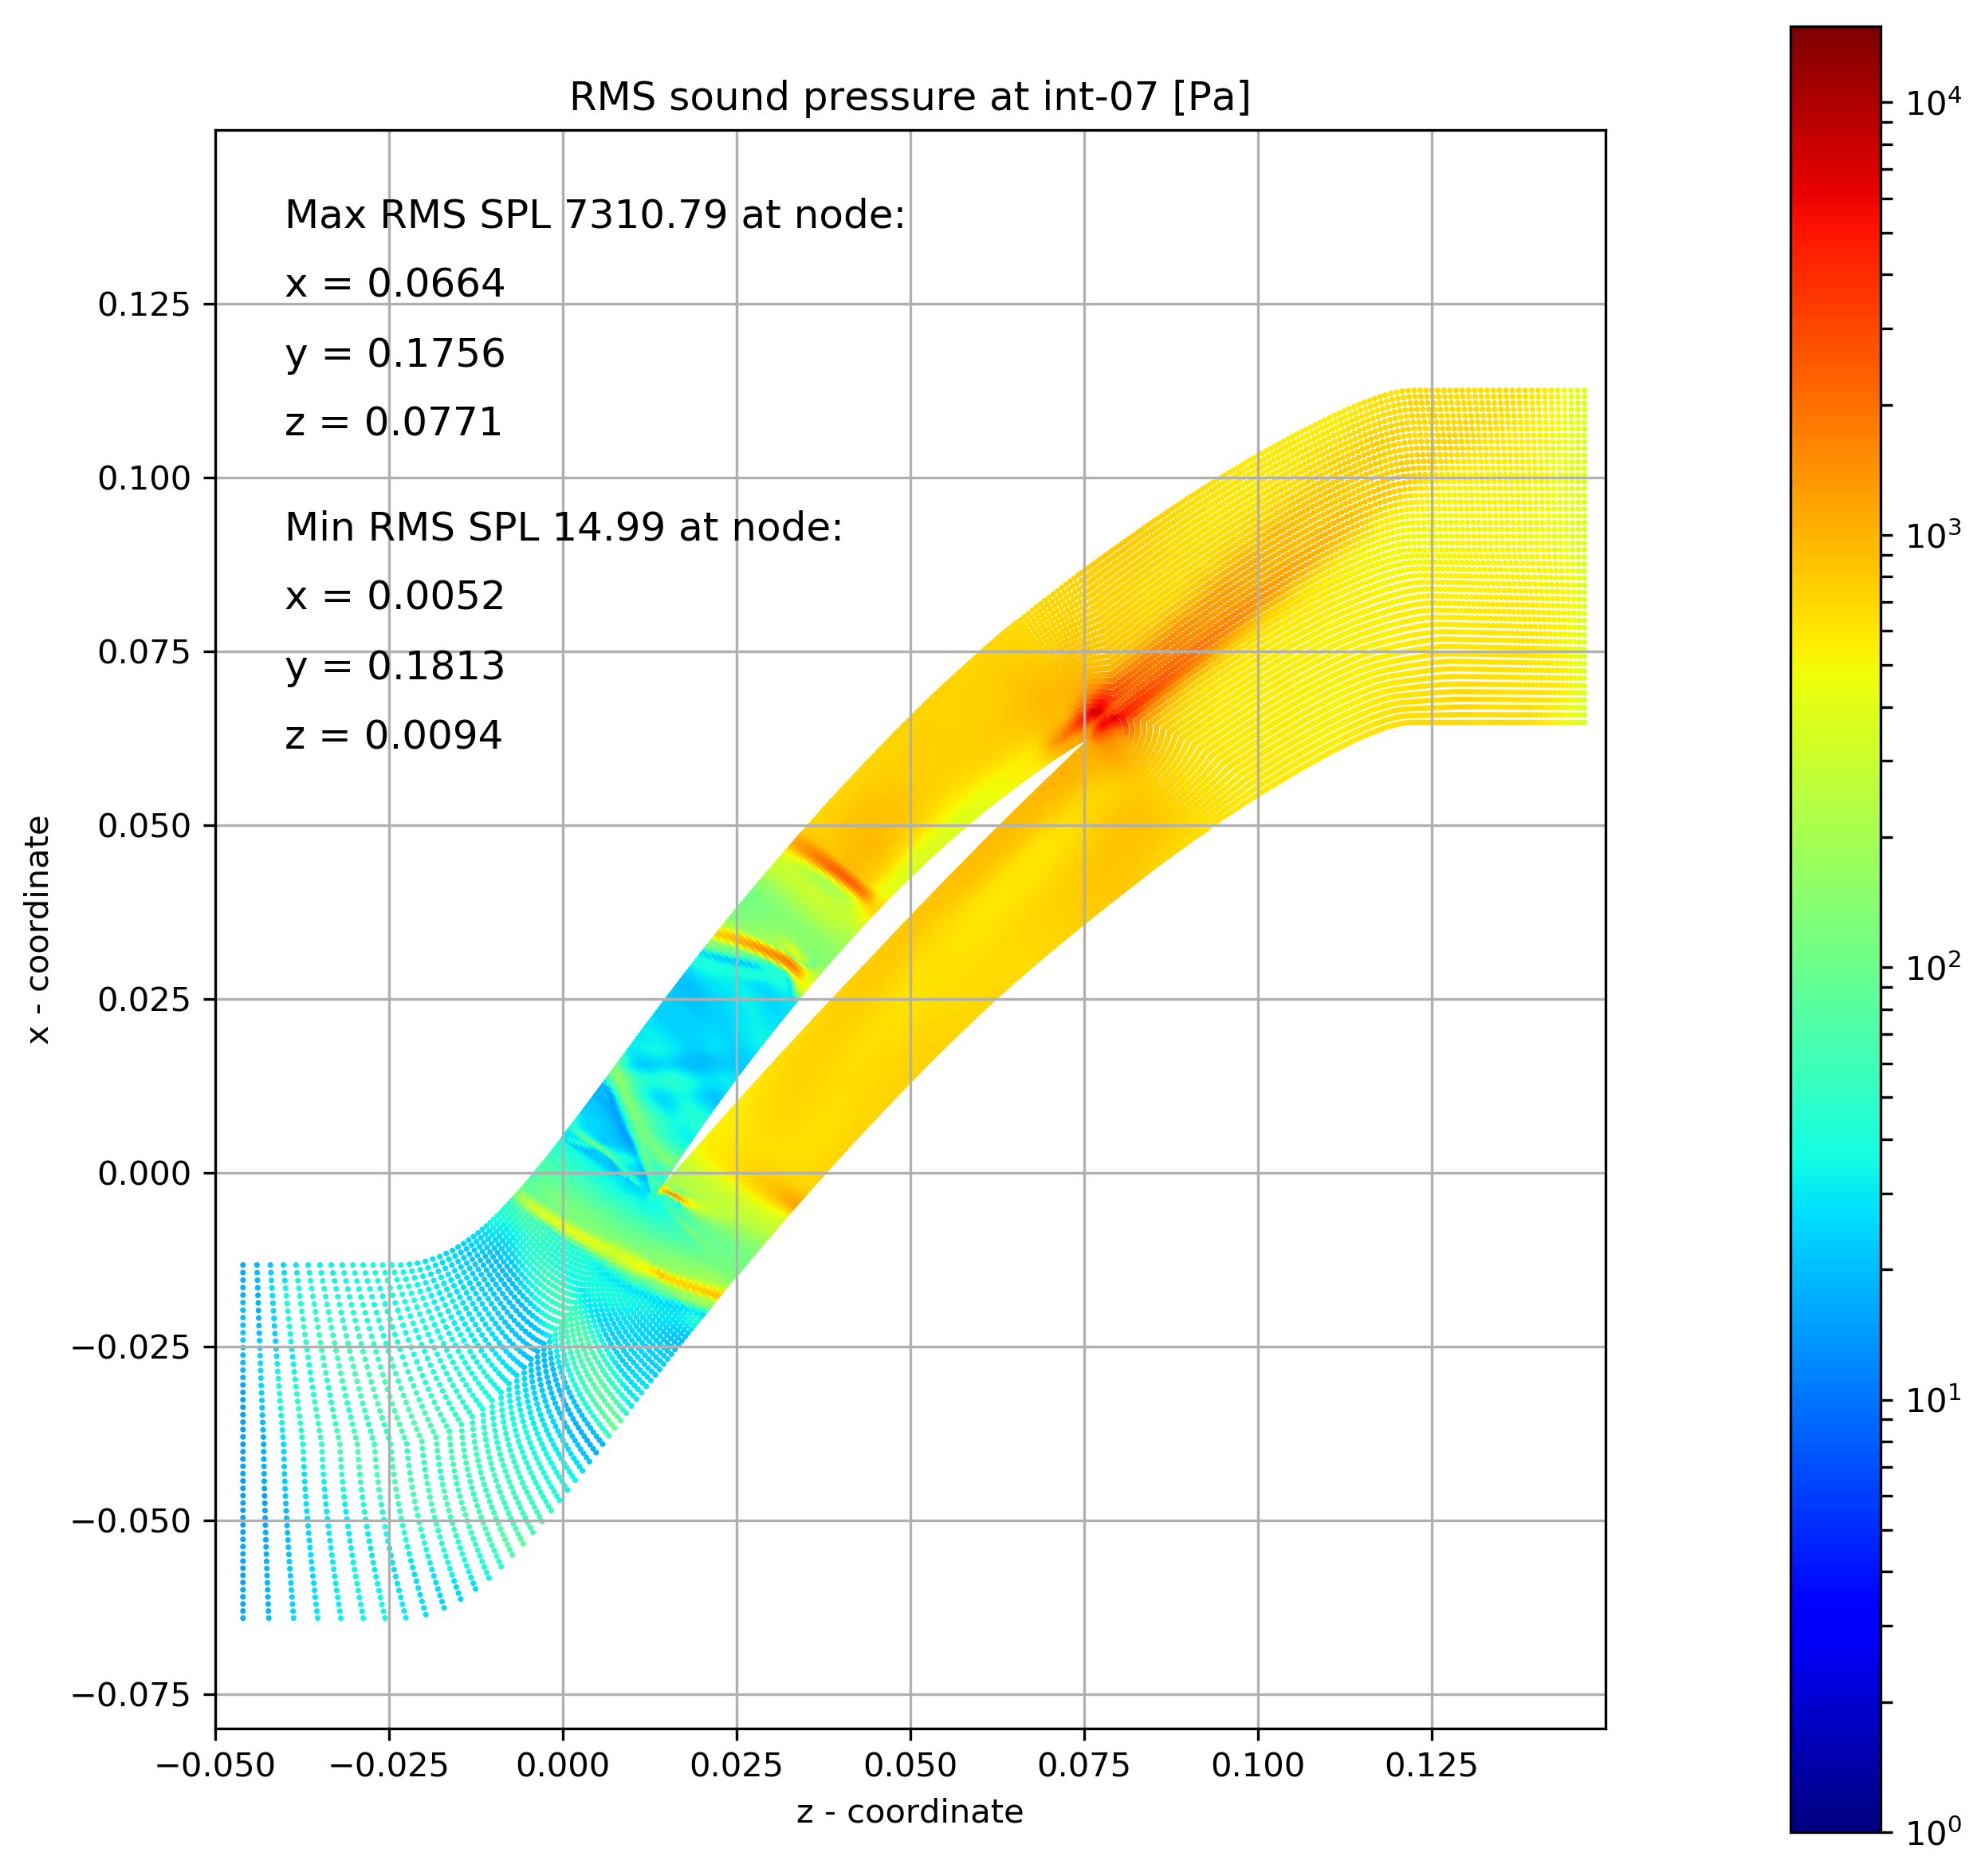
\includegraphics[width=0.75\textwidth]{Figures/int-07-rms-spl.png} \label{int-07-rms-spl}
  \caption{RMS Sound pressure at int-07 mark}
  
  \vspace*{\floatsep}% https://tex.stackexchange.com/q/26521/5764

  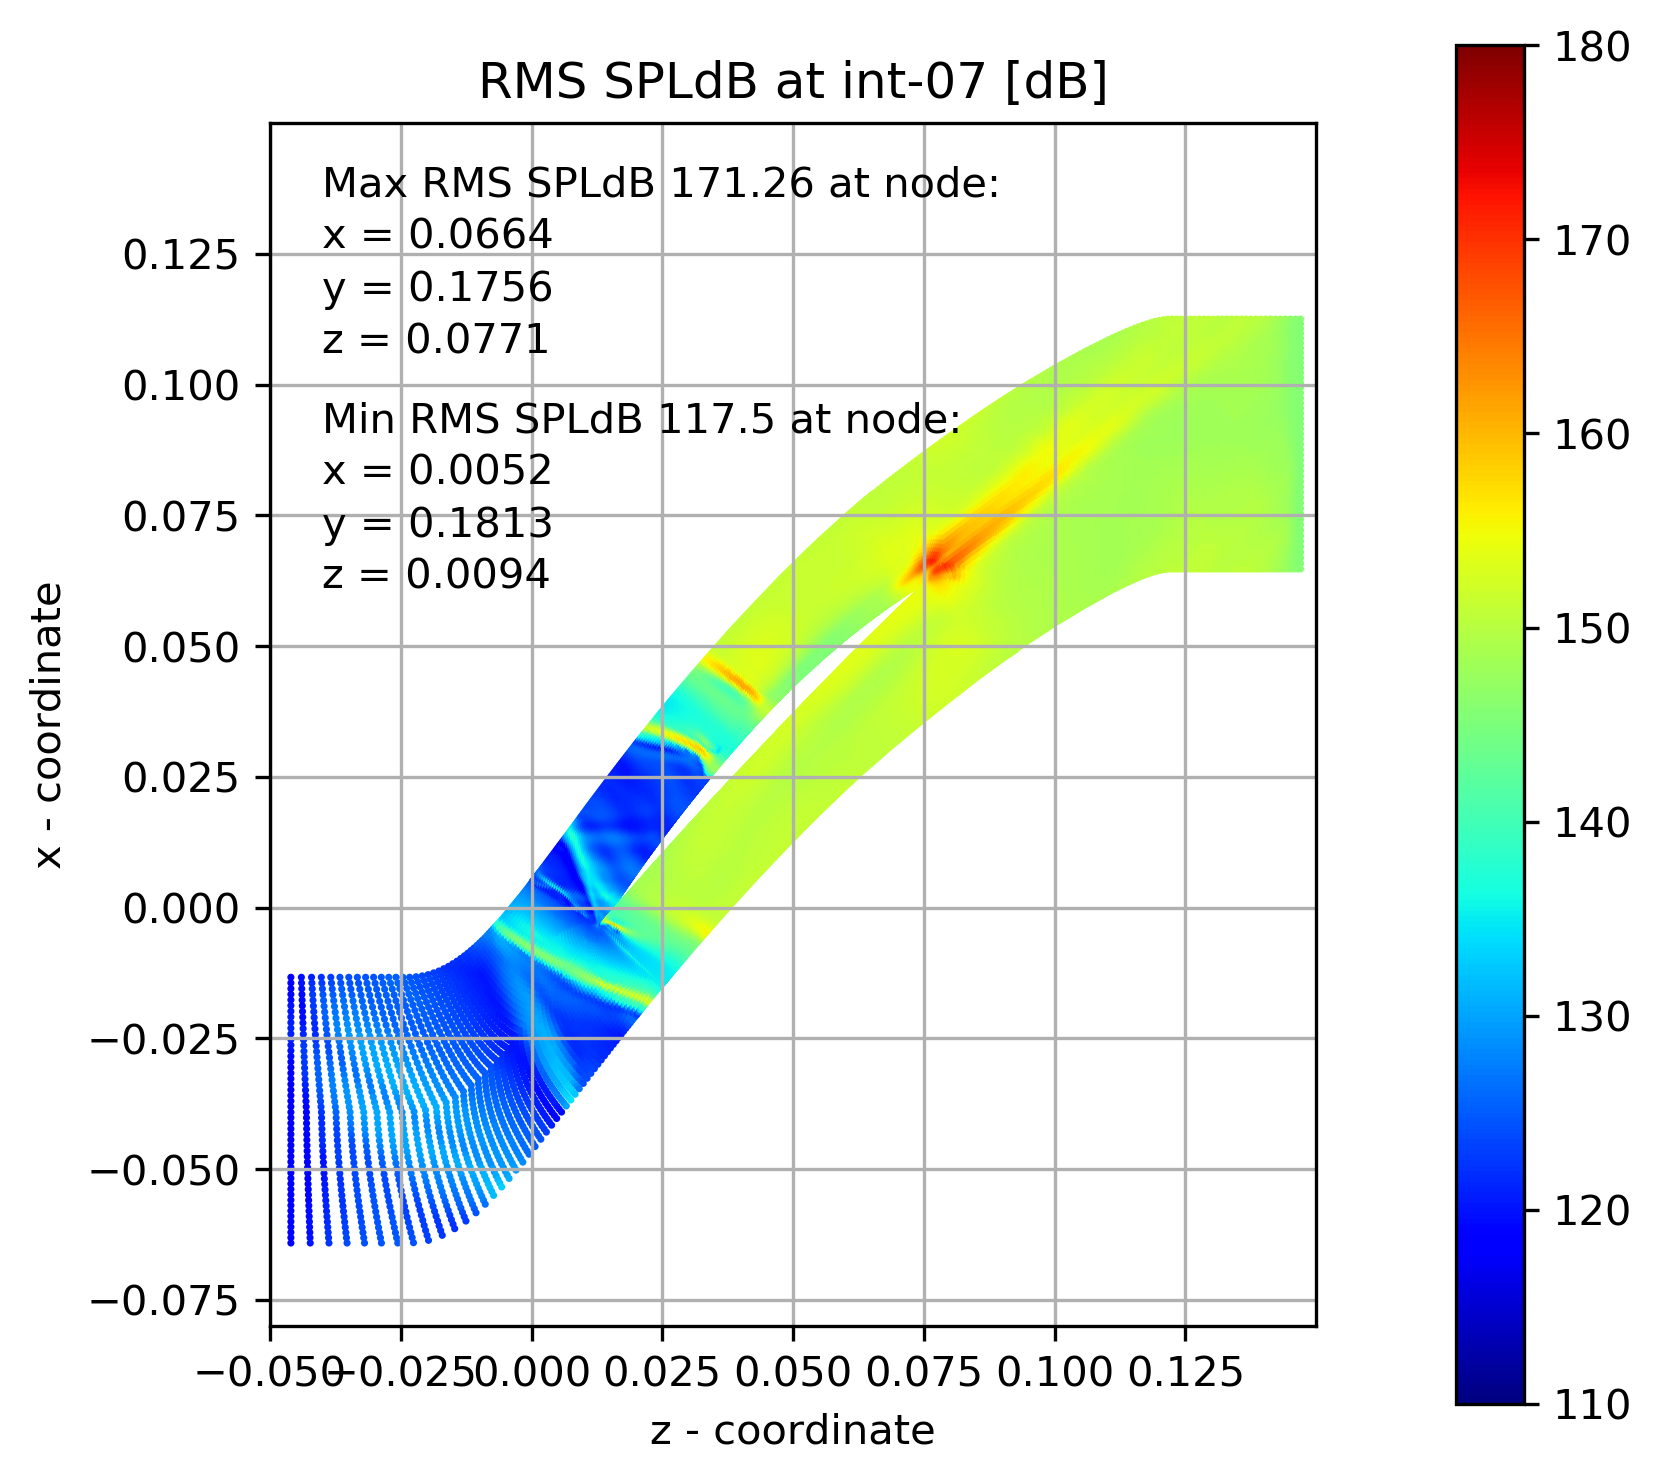
\includegraphics[width=0.75\textwidth]{Figures/int-07-rms-spldb.png} \label{int-07-rms-spldb}
  \caption{RMS Sound pressure decibel level at int-07 mark}
\end{figure}
%int-07
\begin{figure}[ht]
  \centering
  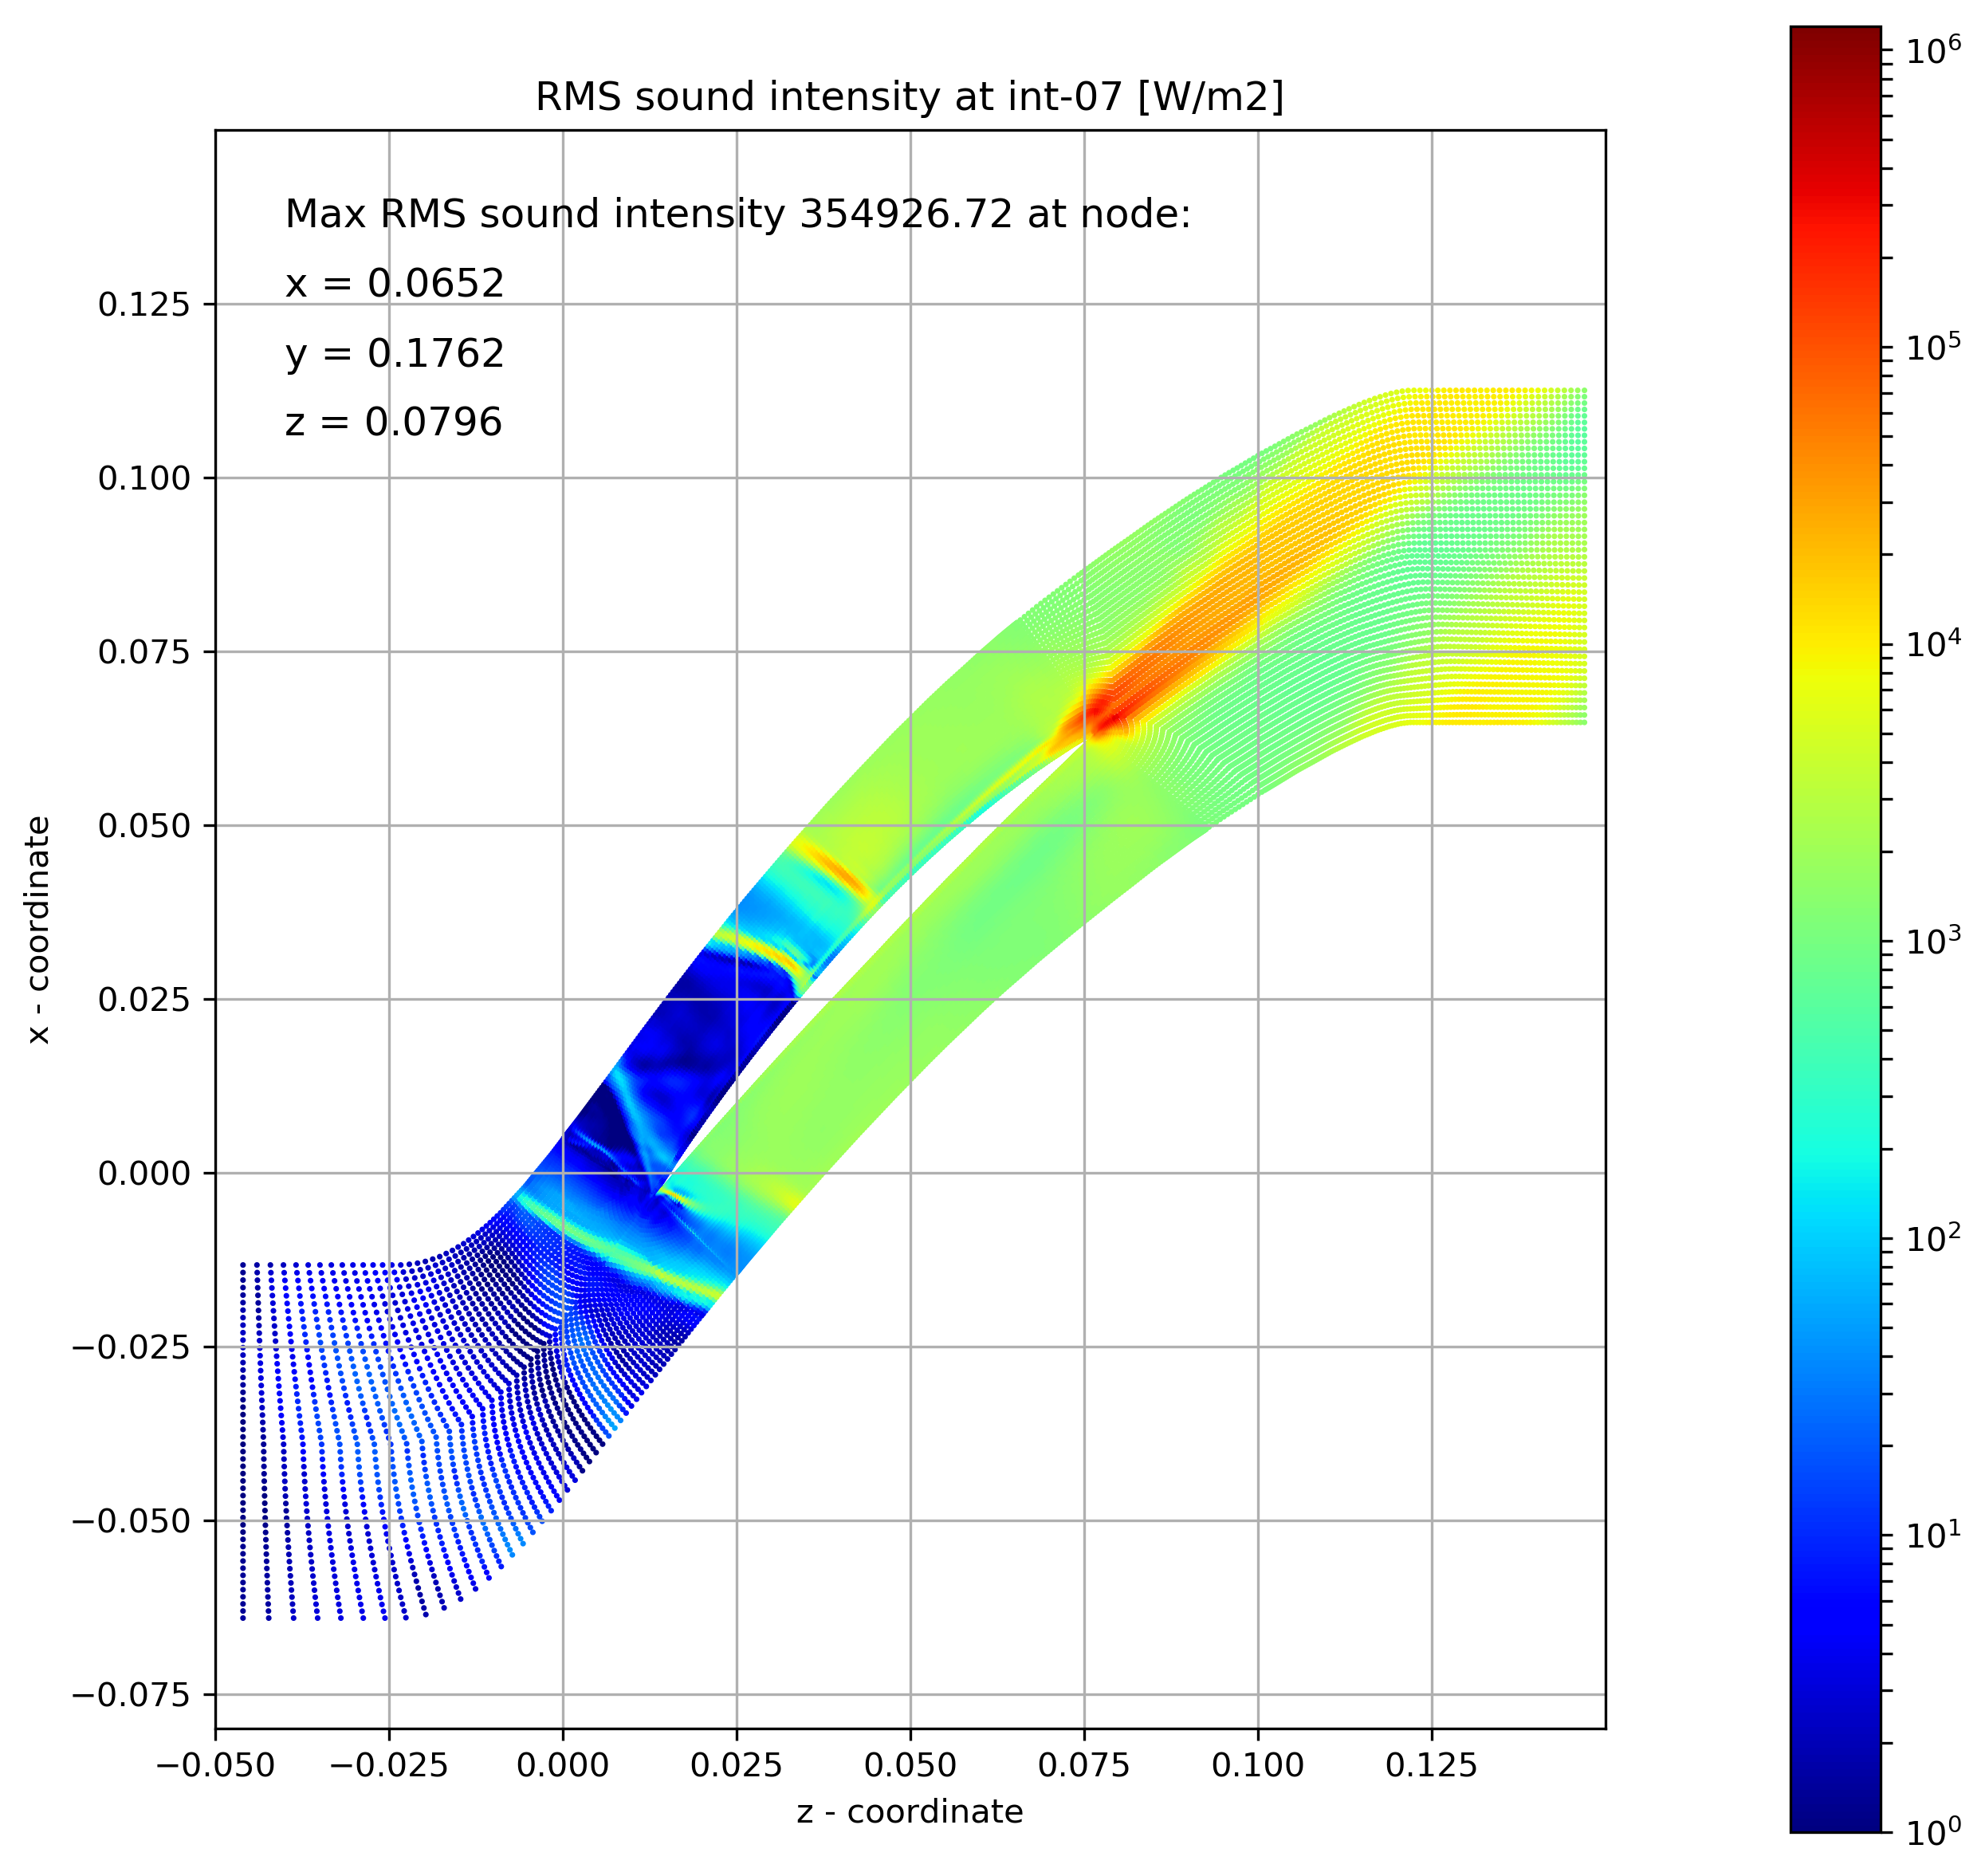
\includegraphics[width=0.75\textwidth]{Figures/int-07-rms-sil.png} \label{int-07-rms-sil}
  \caption{RMS Sound intensity at int-07 mark}
  
  \vspace*{\floatsep}% https://tex.stackexchange.com/q/26521/5764

  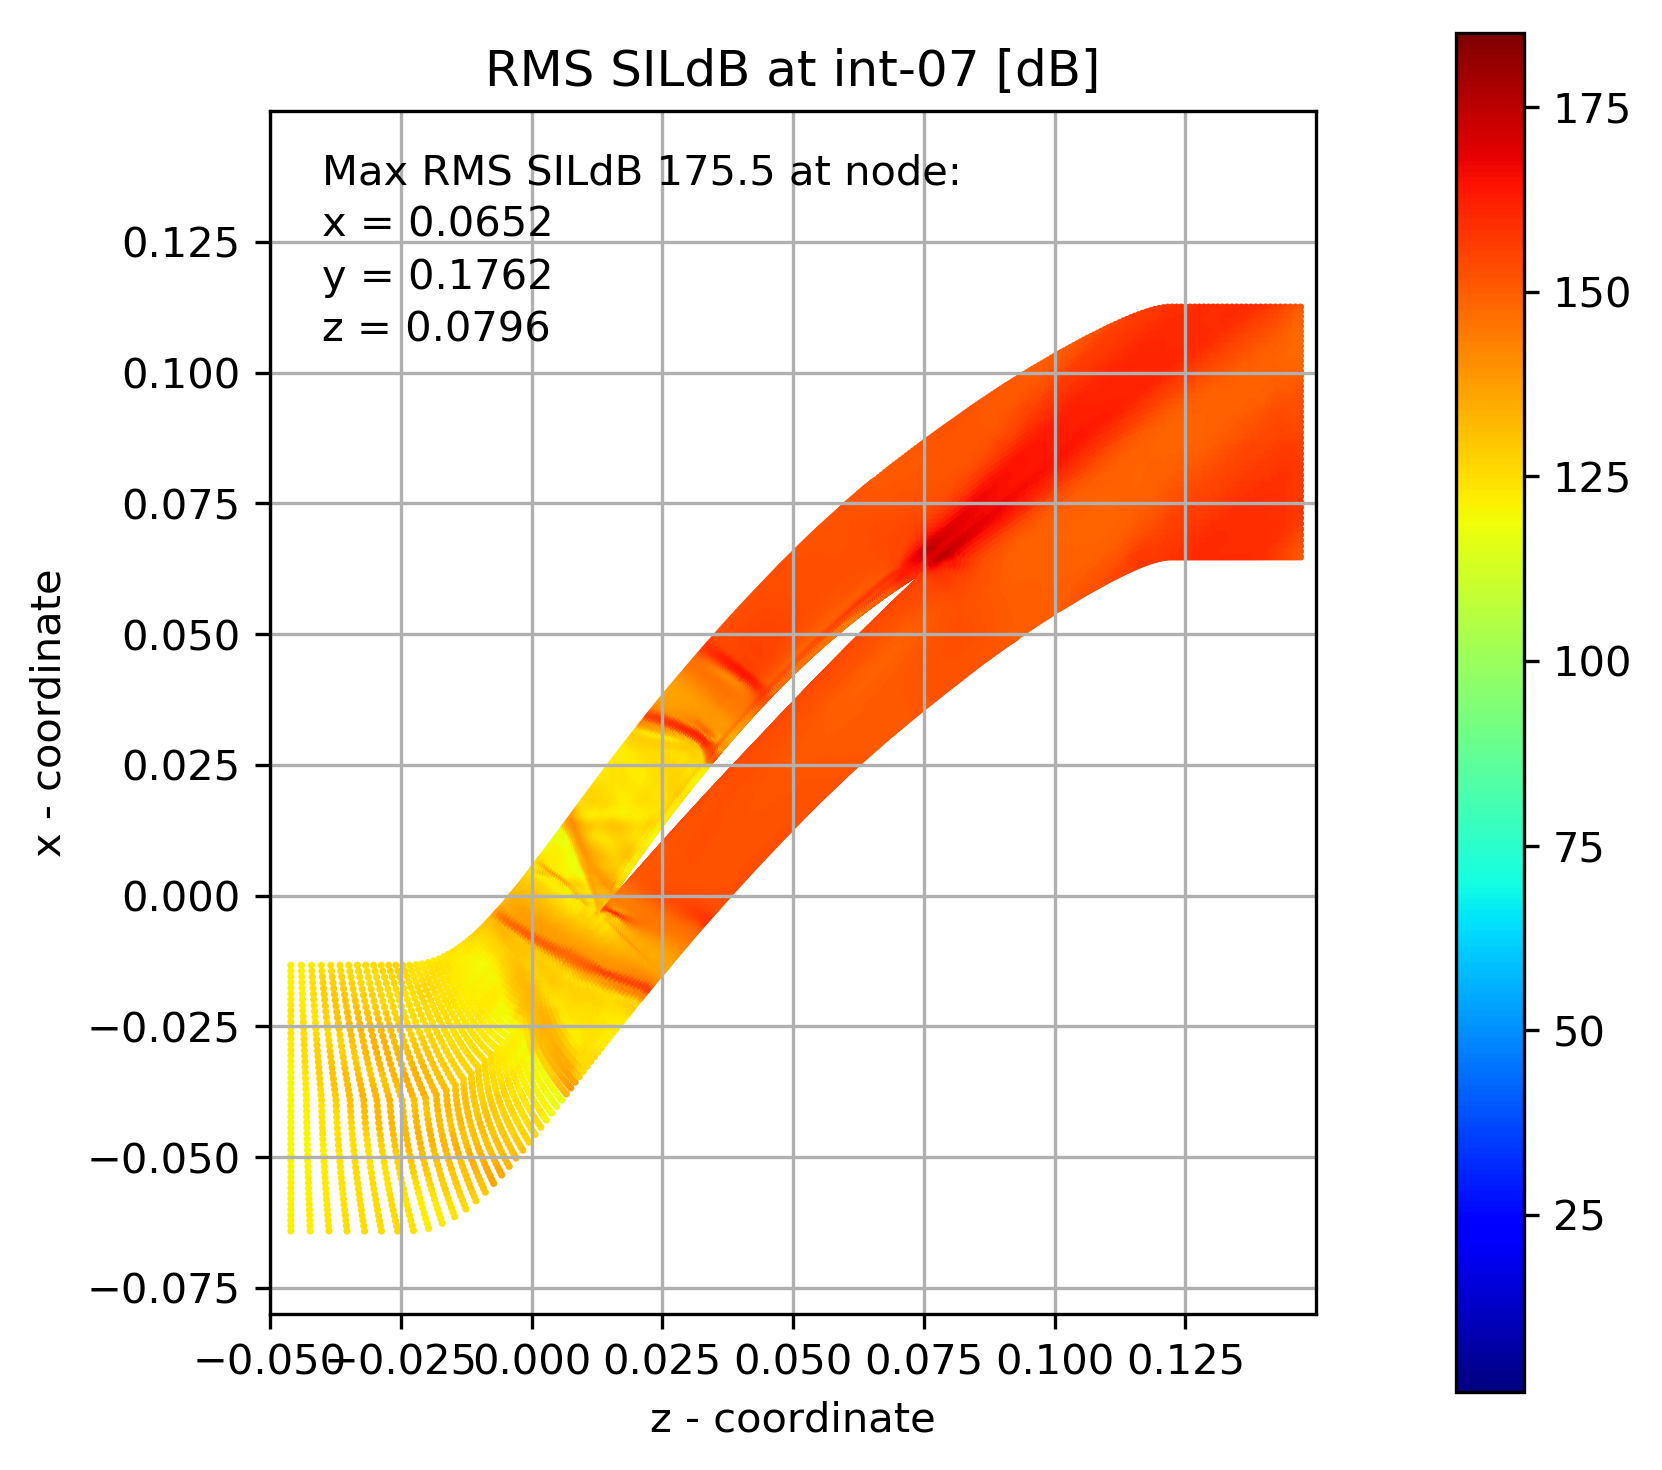
\includegraphics[width=0.75\textwidth]{Figures/int-07-rms-sildb.png} \label{int-07-rms-sildb}
  \caption{RMS Sound intensity decibel level at int-07 mark}
\end{figure}


%int-08
\begin{figure}[ht]
  \centering
  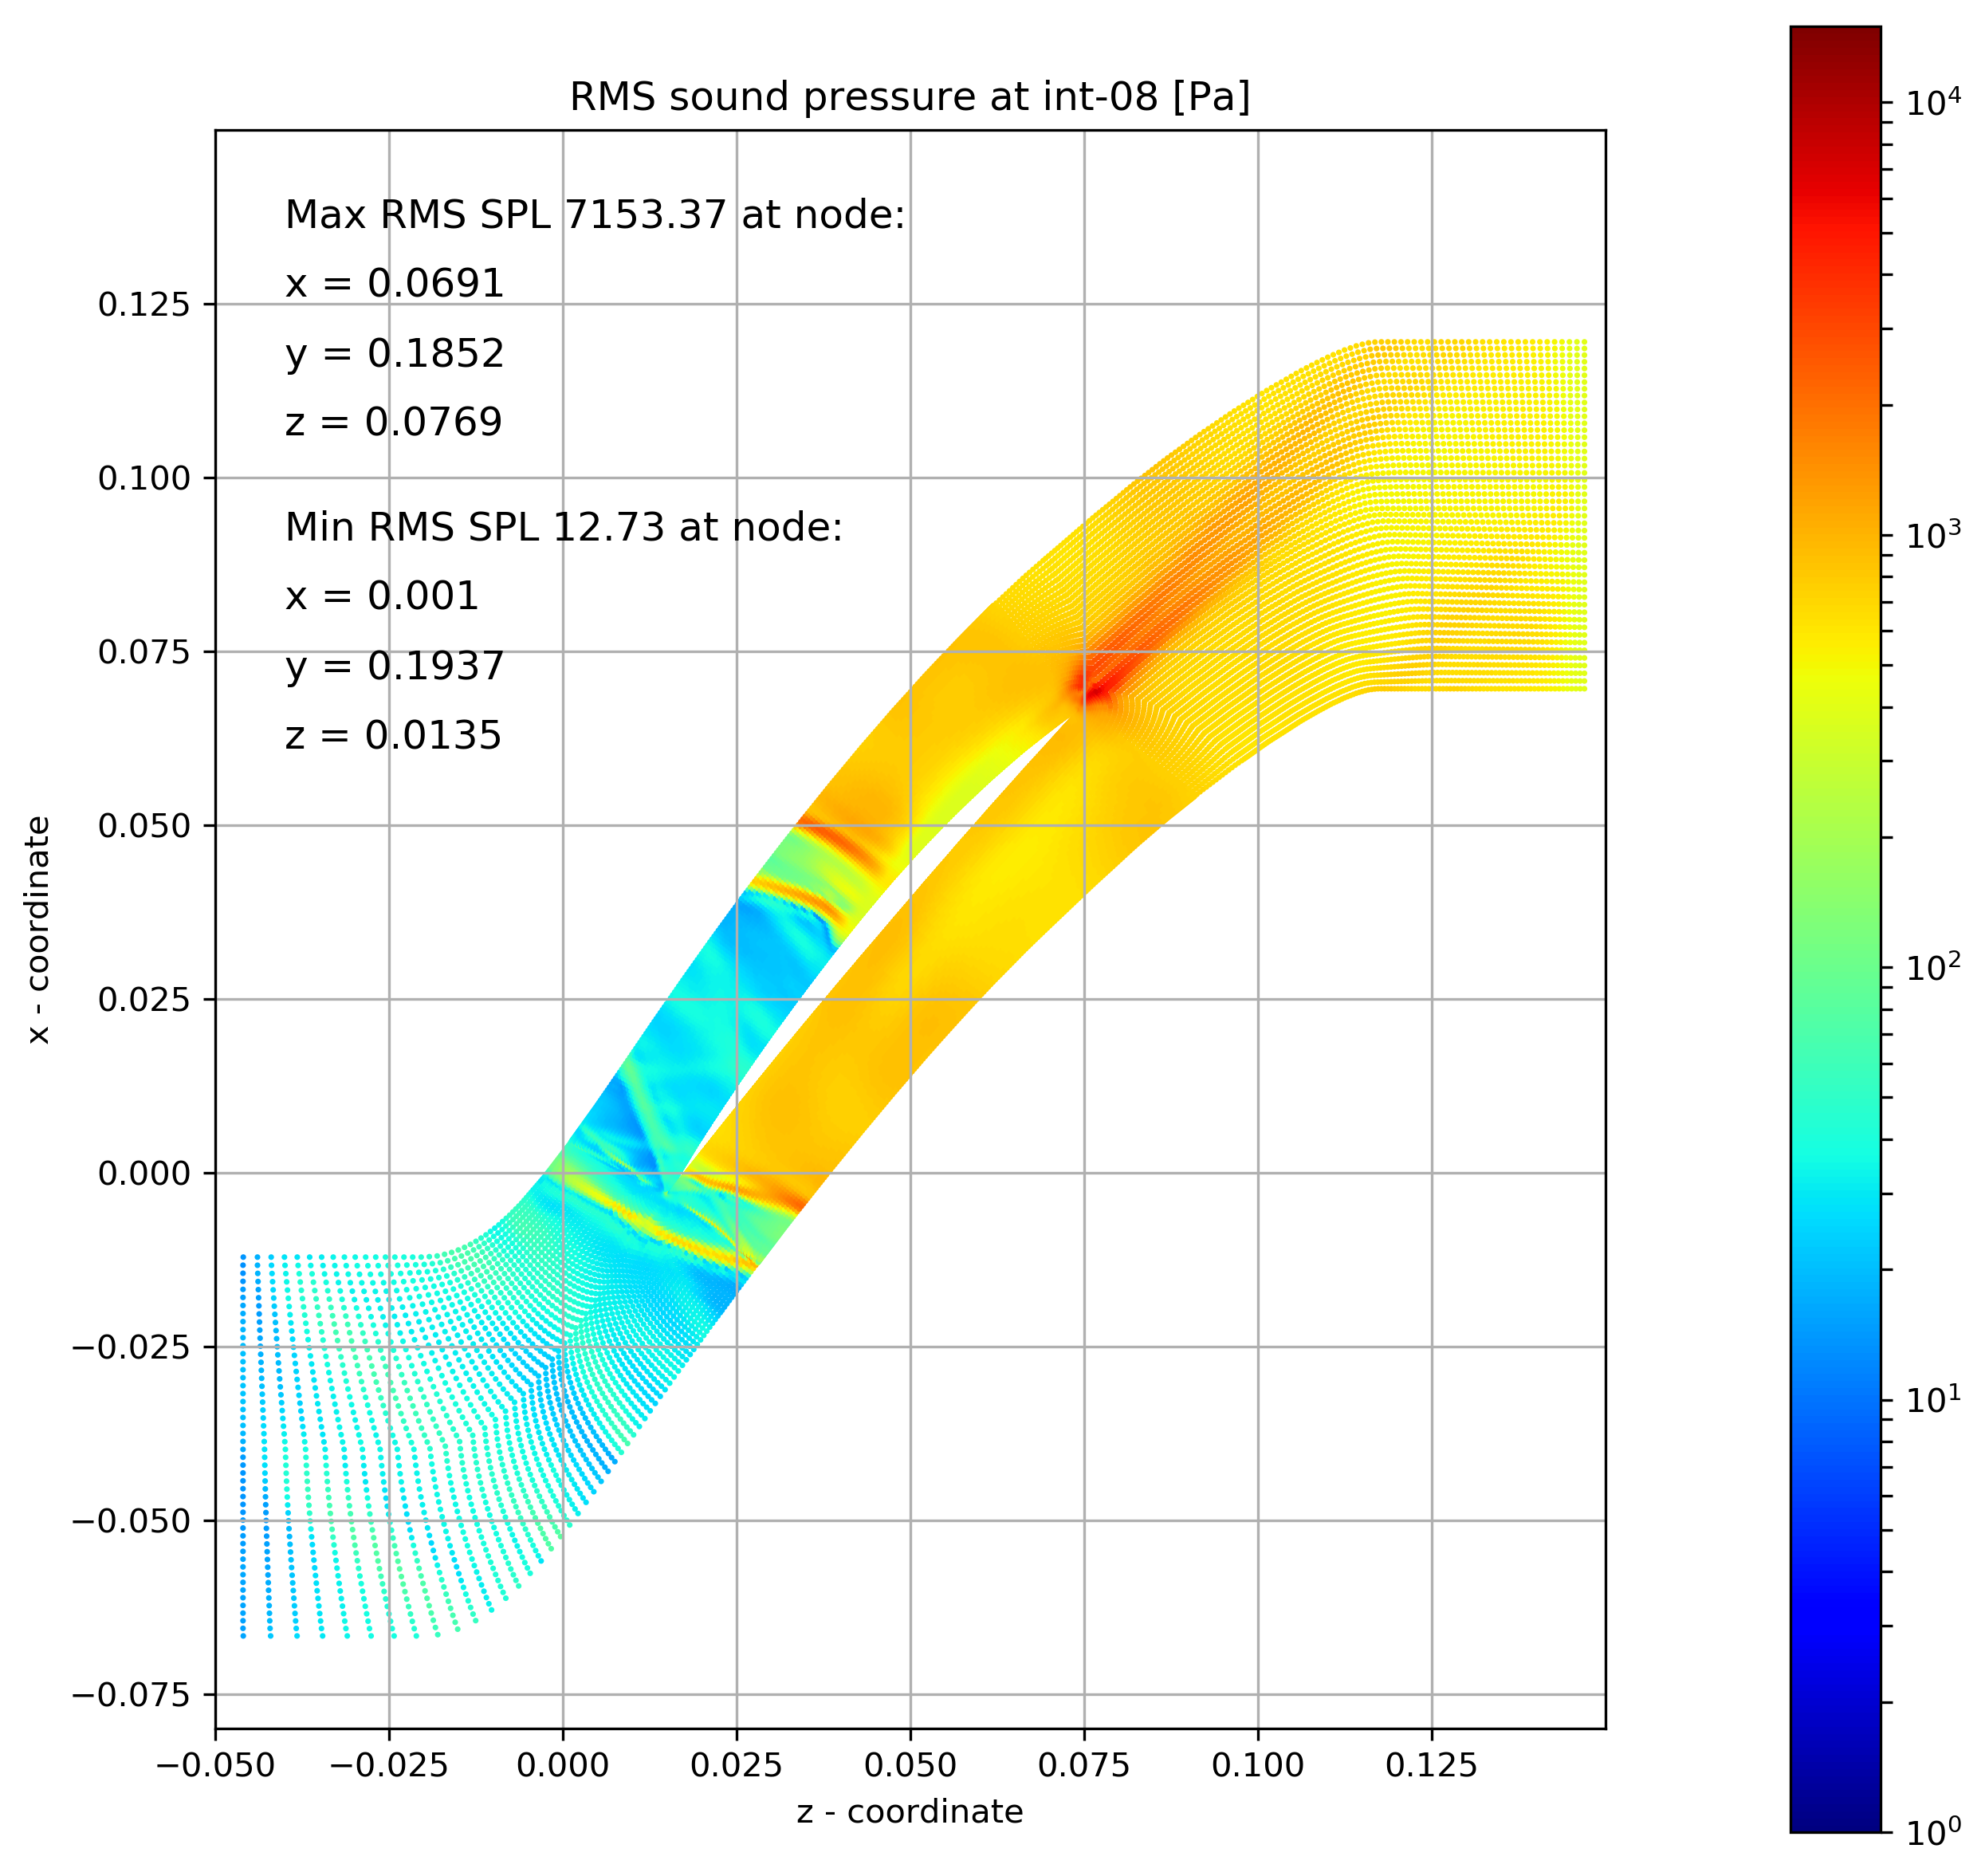
\includegraphics[width=0.75\textwidth]{Figures/int-08-rms-spl.png} \label{int-08-rms-spl}
  \caption{RMS Sound pressure at int-08 mark}
  
  \vspace*{\floatsep}% https://tex.stackexchange.com/q/26521/5764

  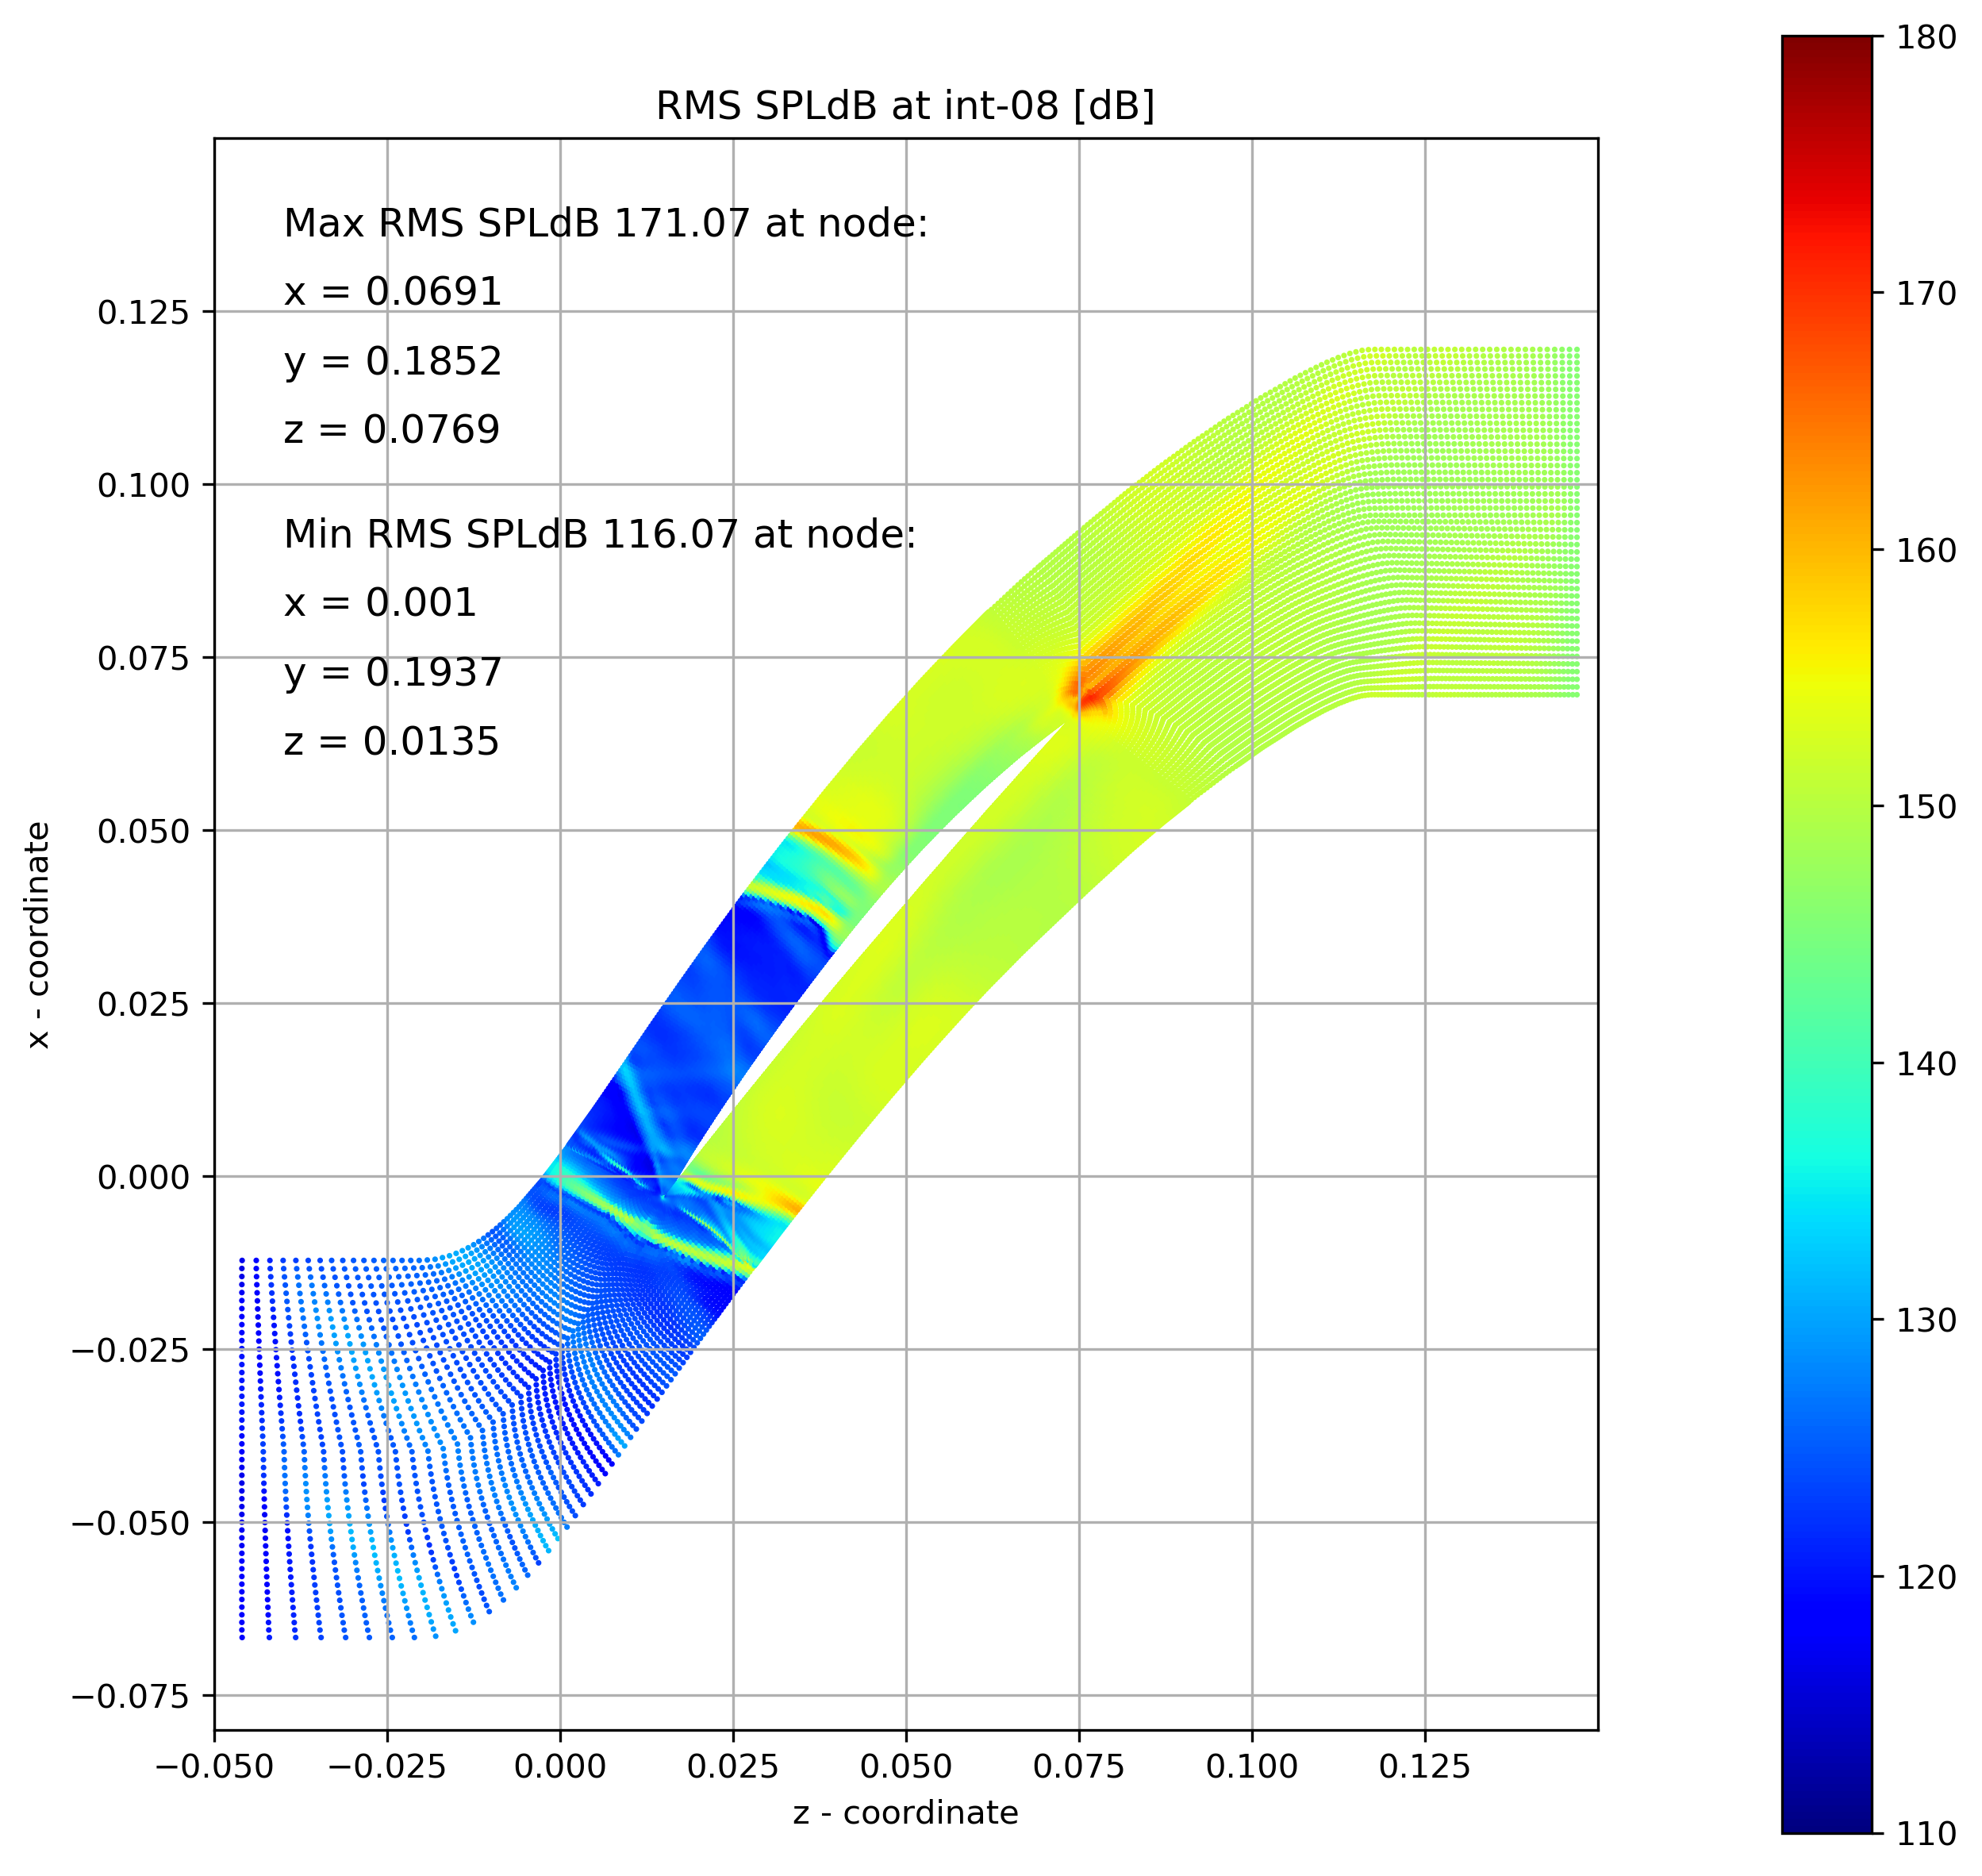
\includegraphics[width=0.75\textwidth]{Figures/int-08-rms-spldb.png} \label{int-08-rms-spldb}
  \caption{RMS Sound pressure decibel level at int-08 mark}
\end{figure}
%int-08
\begin{figure}[ht]
  \centering
  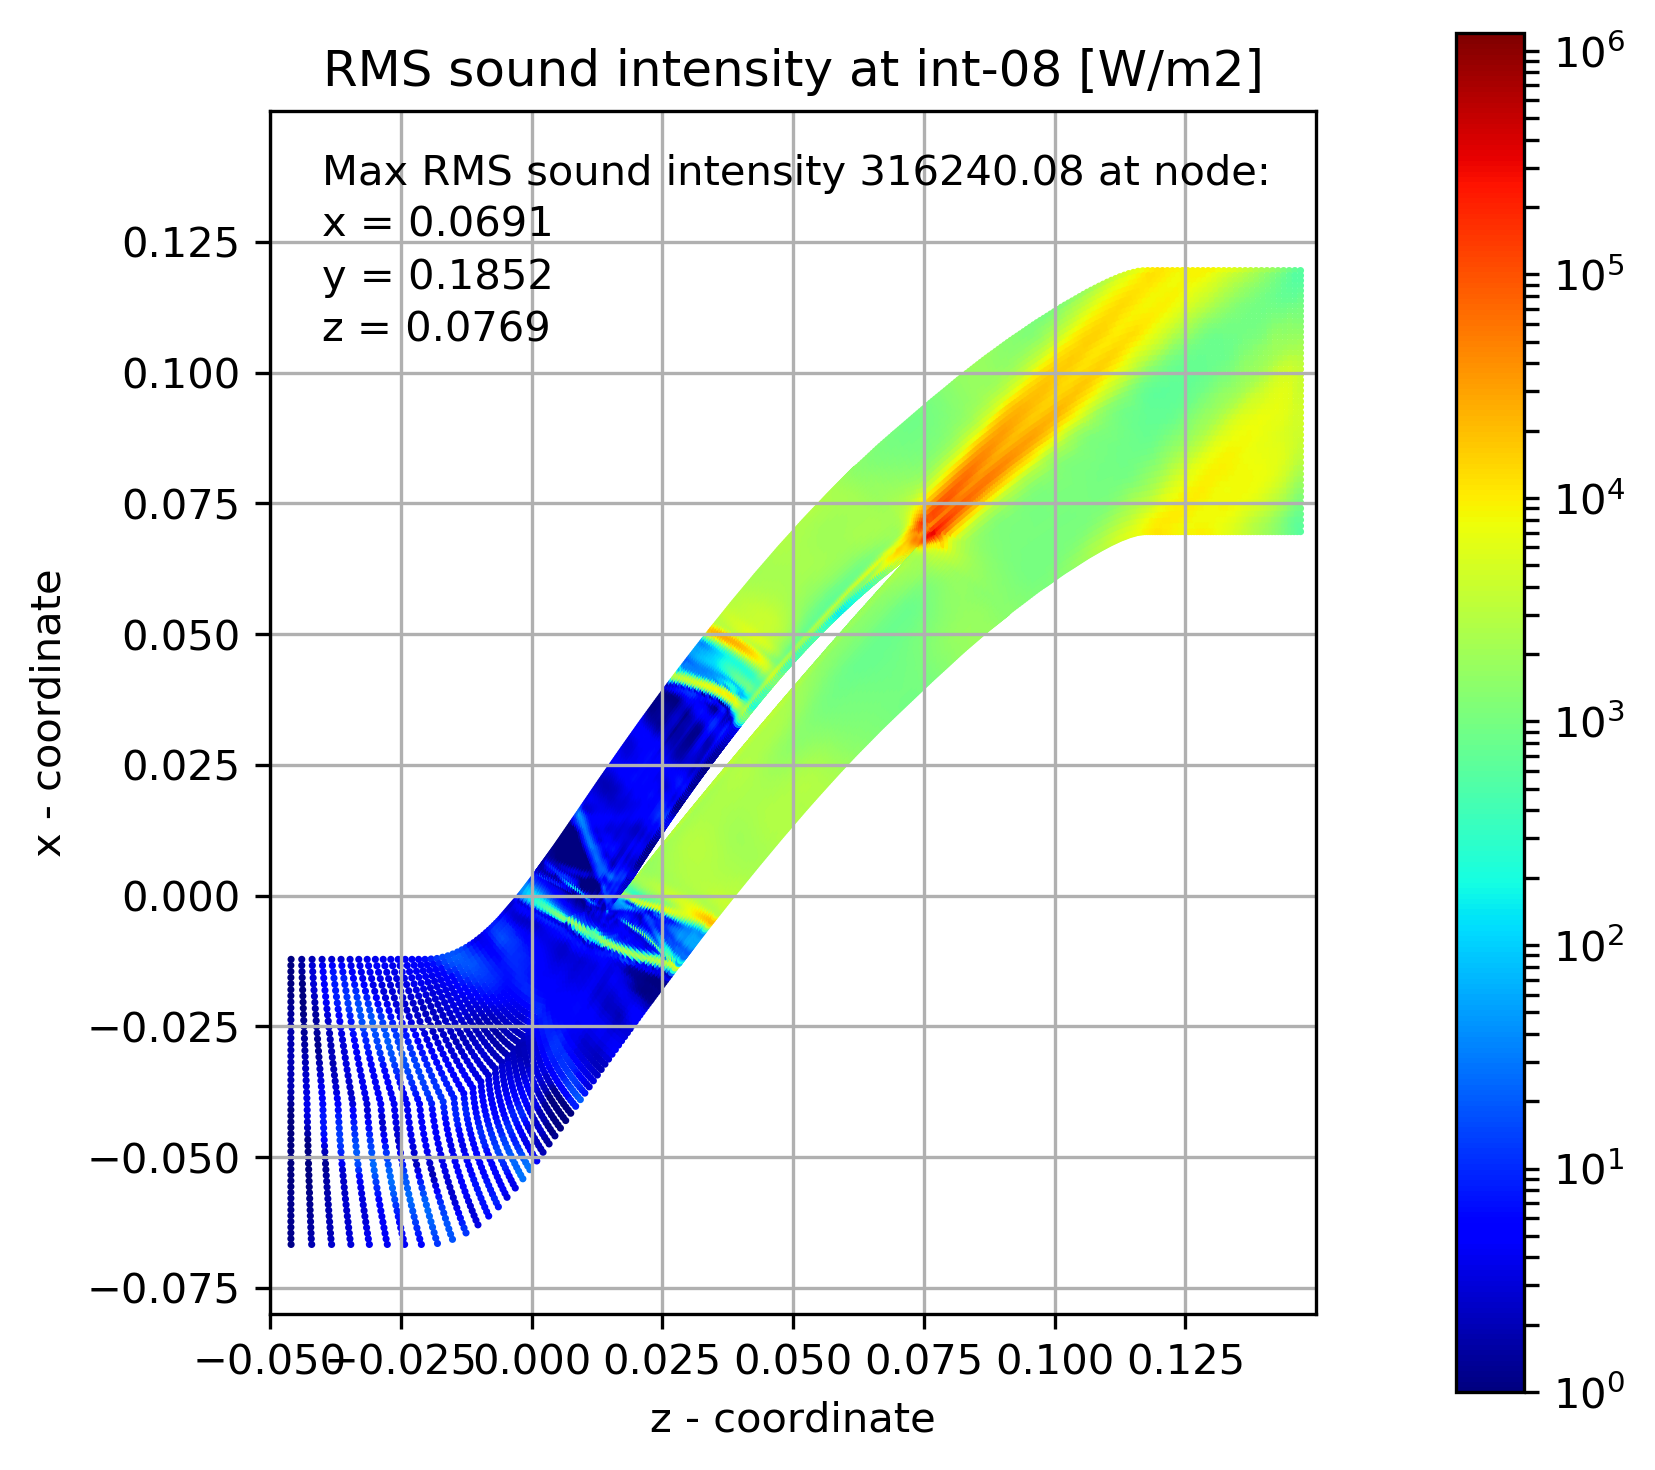
\includegraphics[width=0.75\textwidth]{Figures/int-08-rms-sil.png} \label{int-08-rms-sil}
  \caption{RMS Sound intensity at int-08 mark}
  
  \vspace*{\floatsep}% https://tex.stackexchange.com/q/26521/5764

  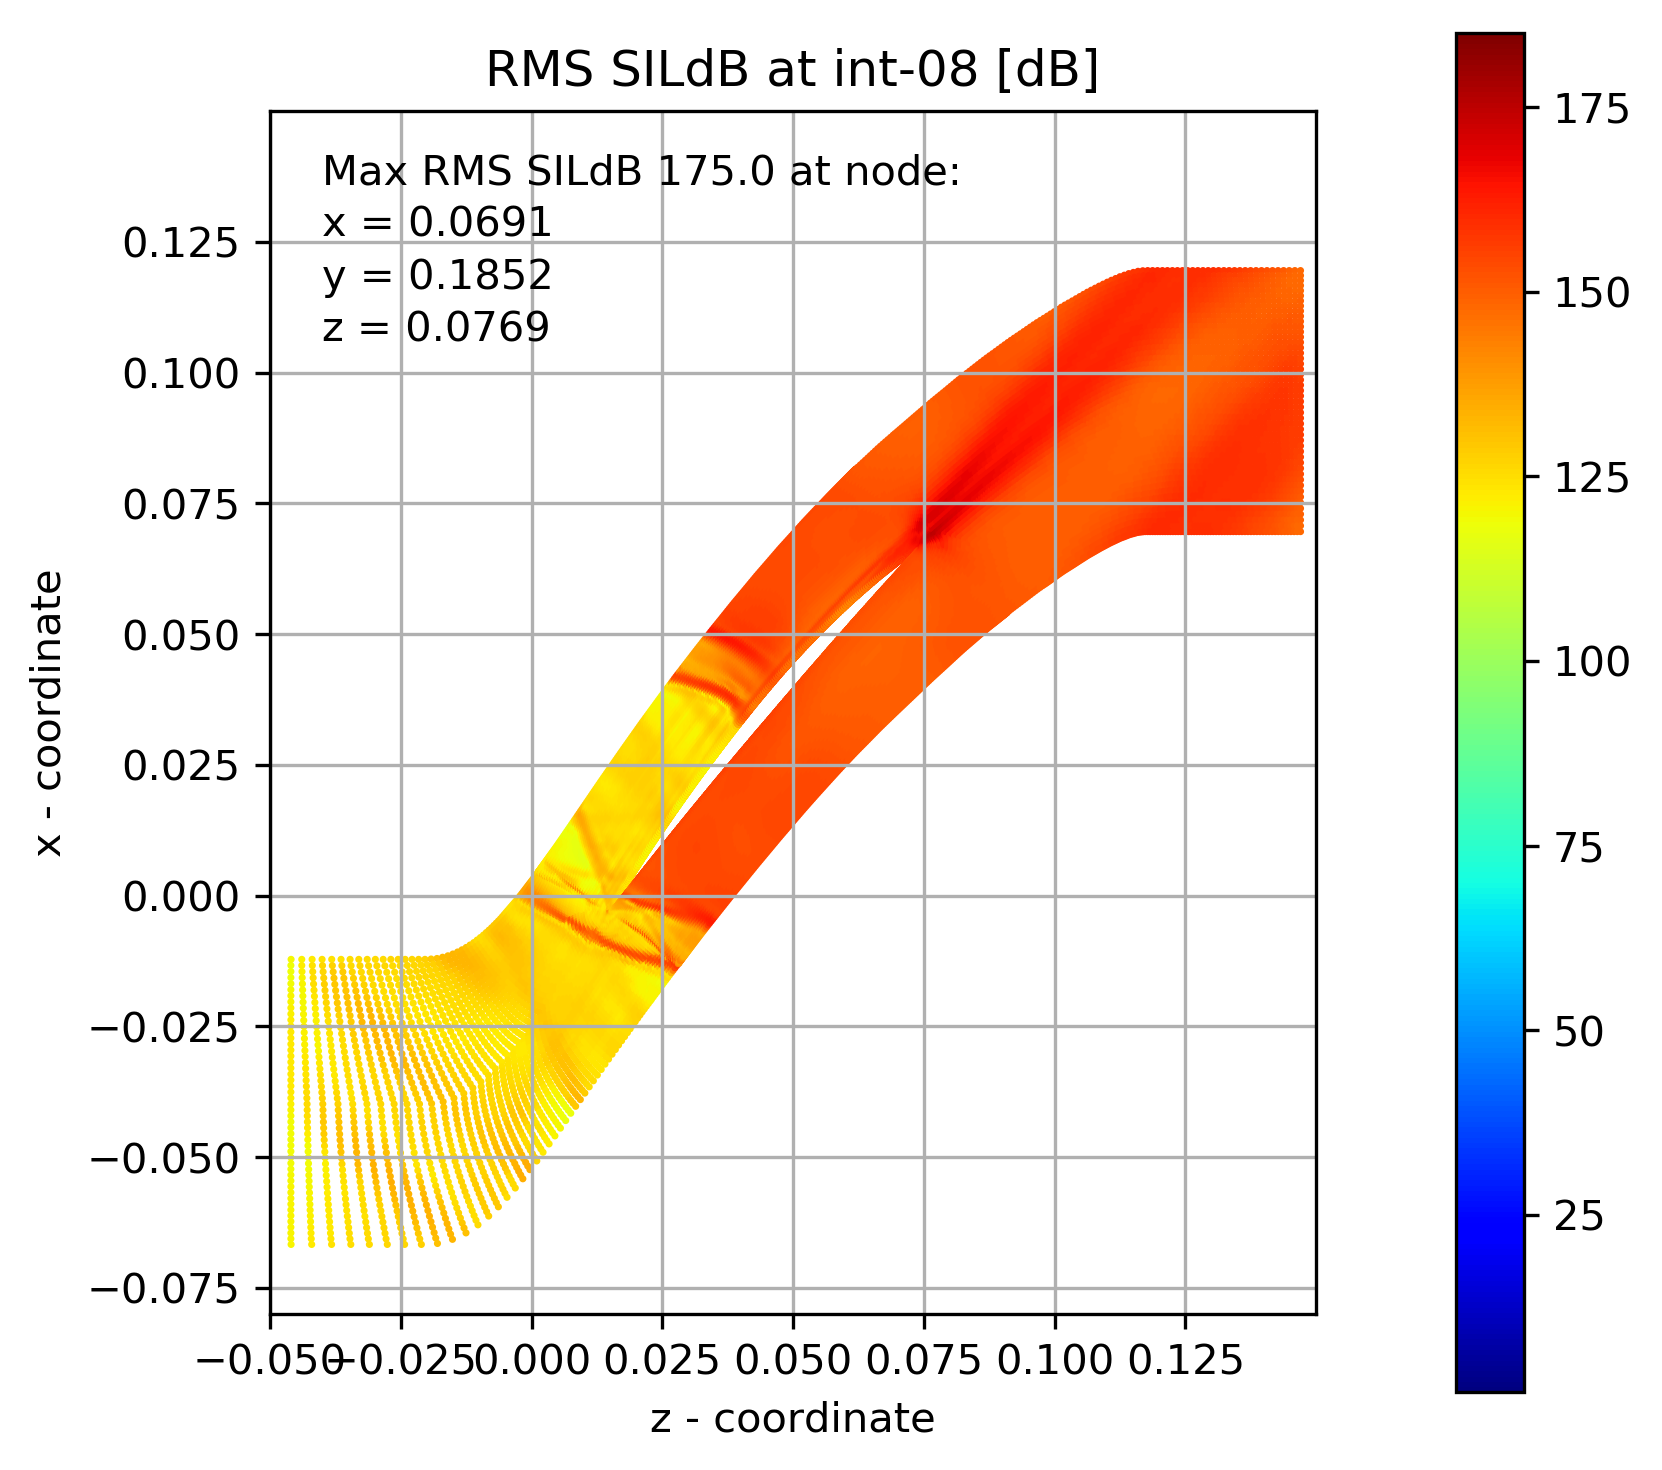
\includegraphics[width=0.75\textwidth]{Figures/int-08-rms-sildb.png} \label{int-08-rms-sildb}
  \caption{RMS Sound intensity decibel level at int-08 mark}
\end{figure}


%int-09
\begin{figure}[ht]
  \centering
  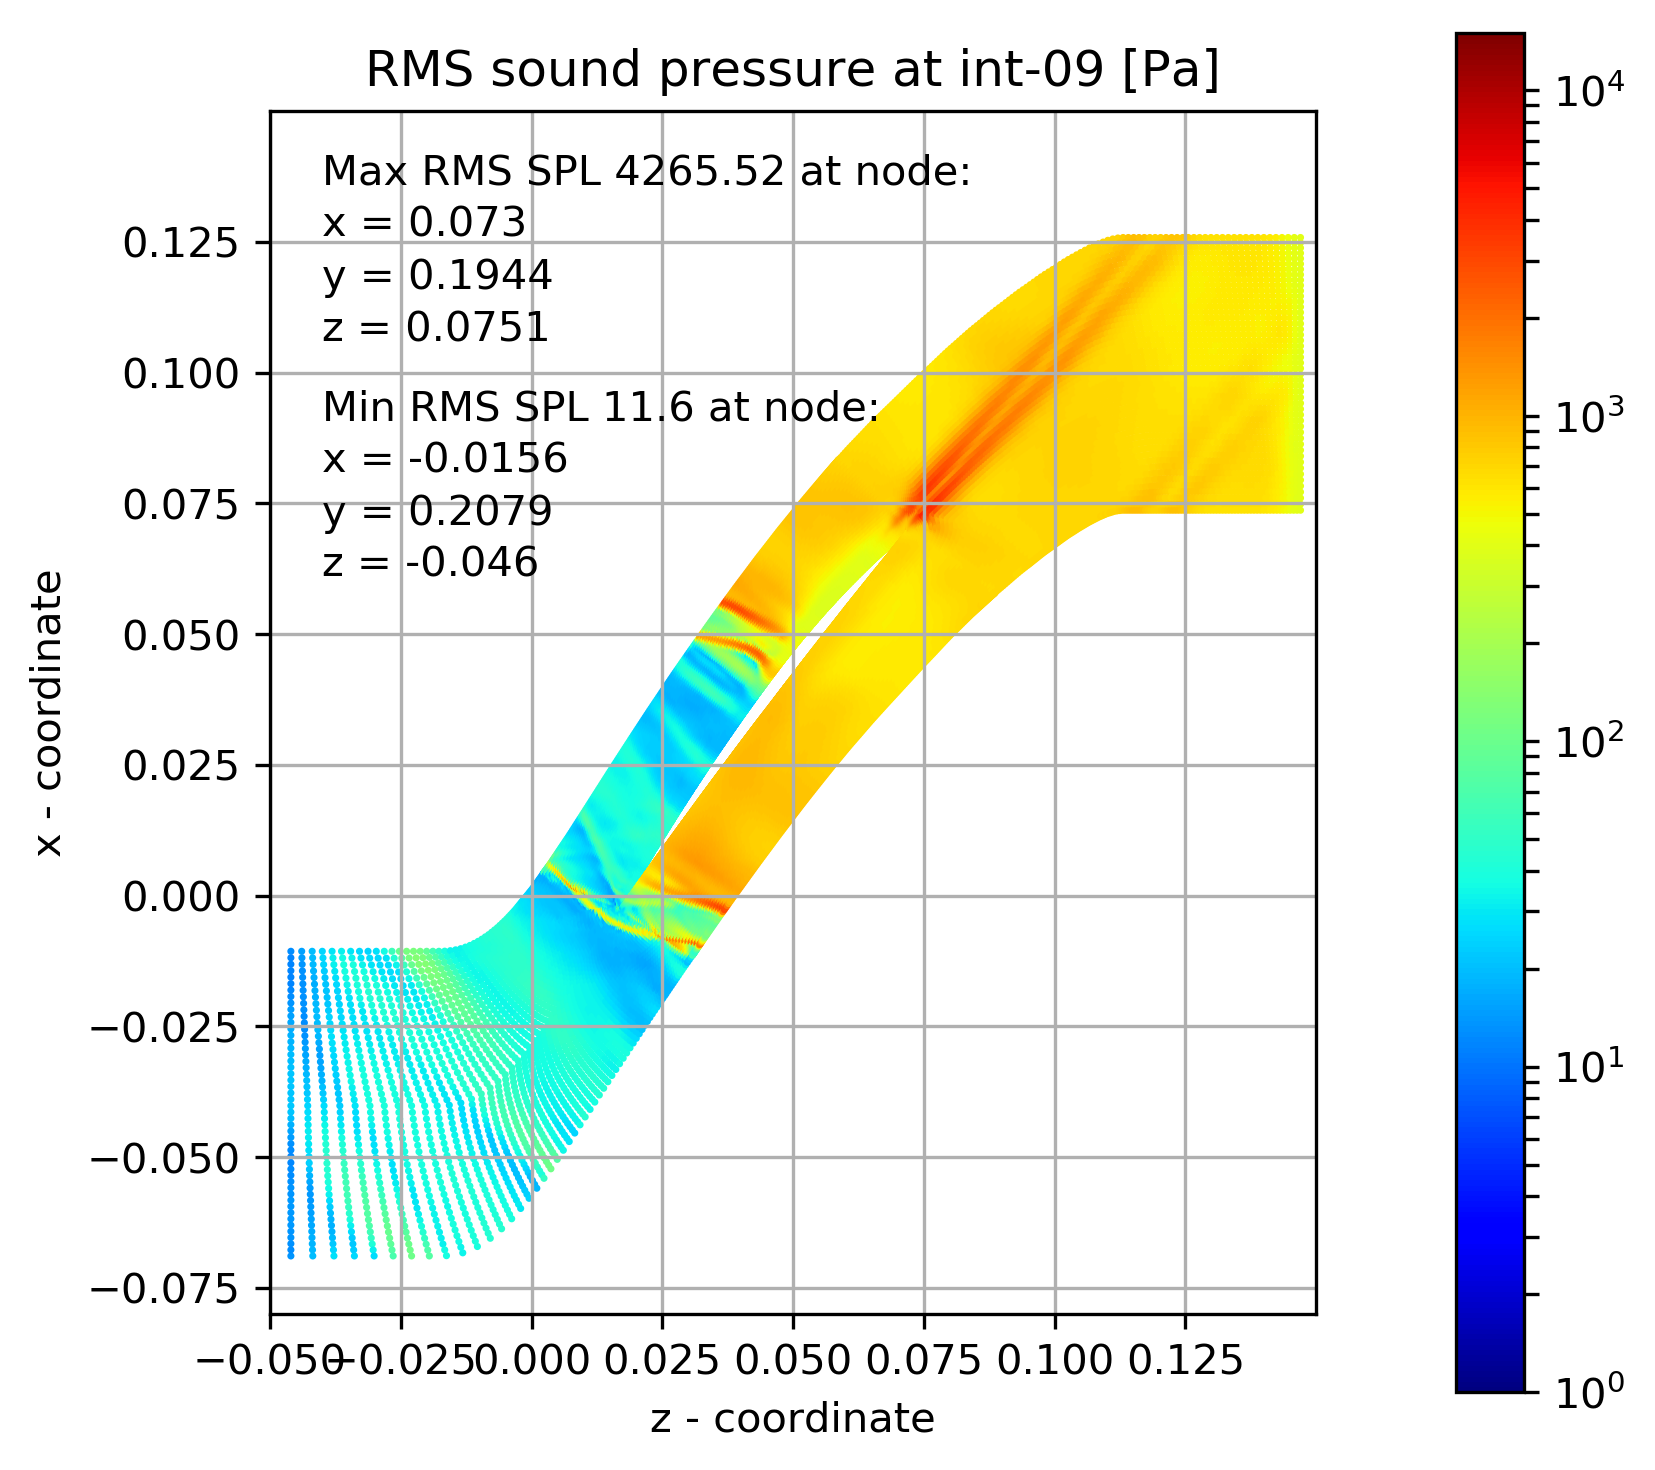
\includegraphics[width=0.75\textwidth]{Figures/int-09-rms-spl.png} \label{int-09-rms-spl}
  \caption{RMS Sound pressure at int-09 mark}
  
  \vspace*{\floatsep}% https://tex.stackexchange.com/q/26521/5764

  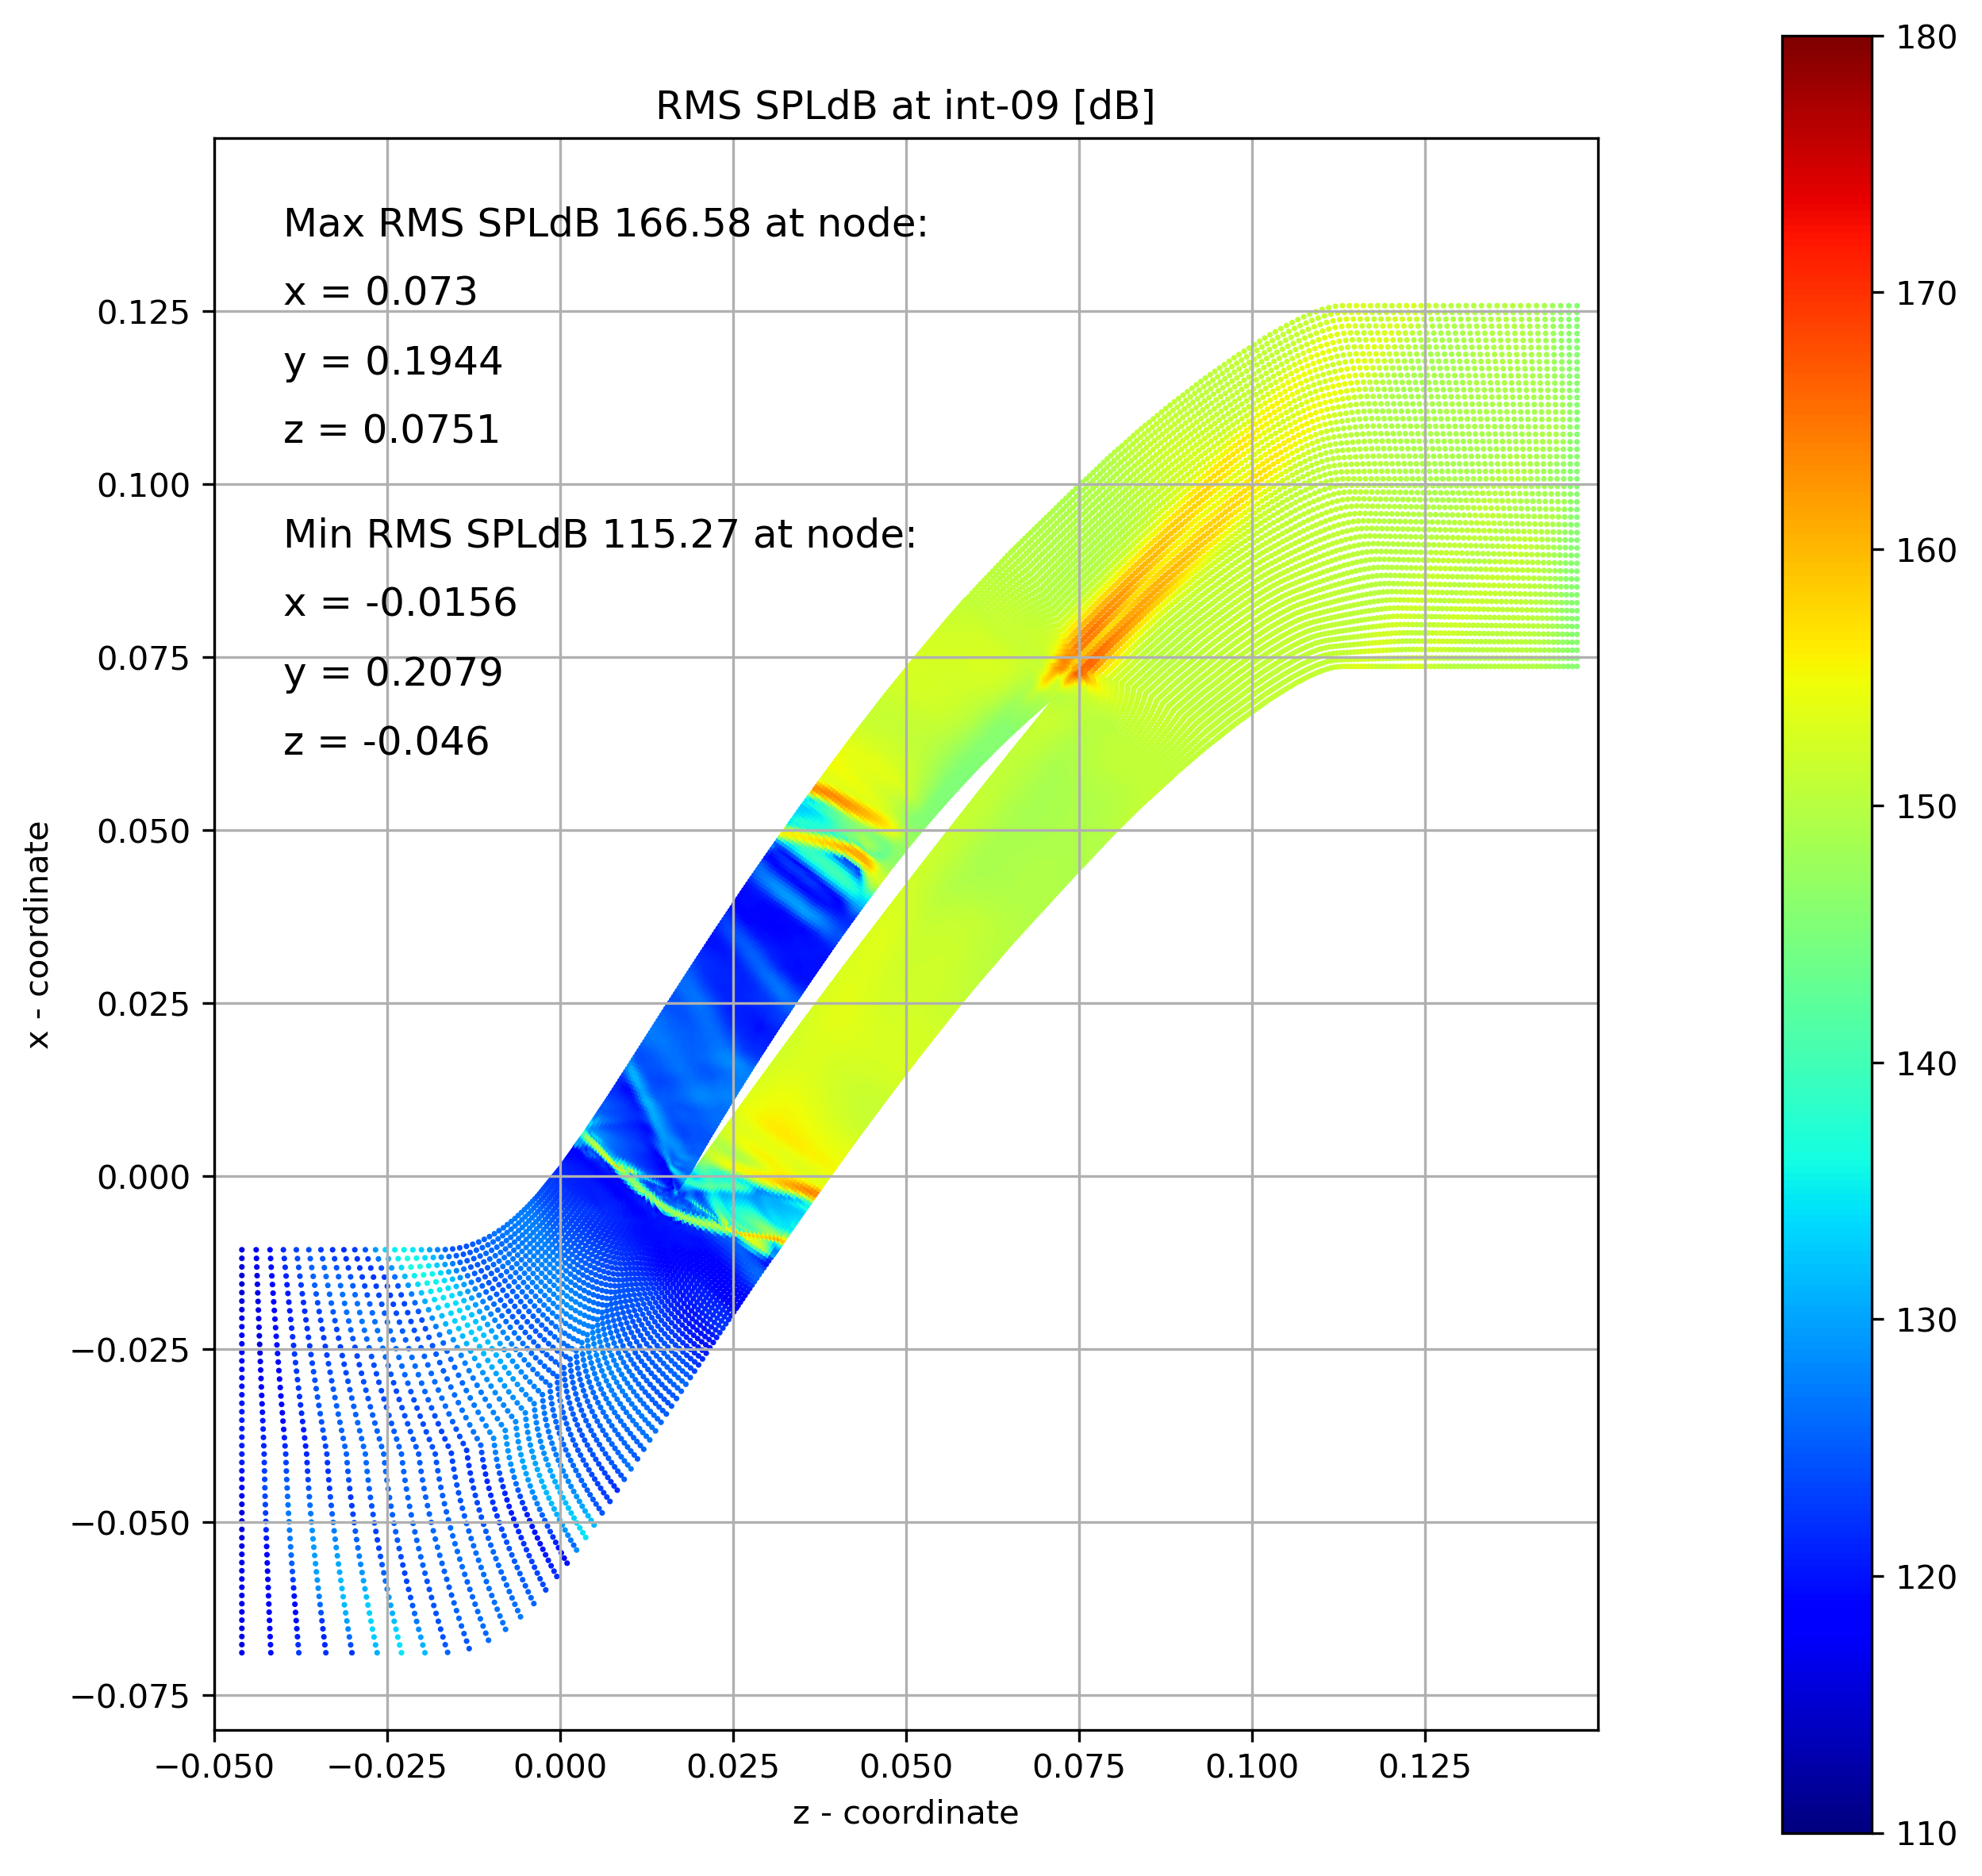
\includegraphics[width=0.75\textwidth]{Figures/int-09-rms-spldb.png} \label{int-09-rms-spldb}
  \caption{RMS Sound pressure decibel level at int-09 mark}
\end{figure}
%int-09
\begin{figure}[ht]
  \centering
  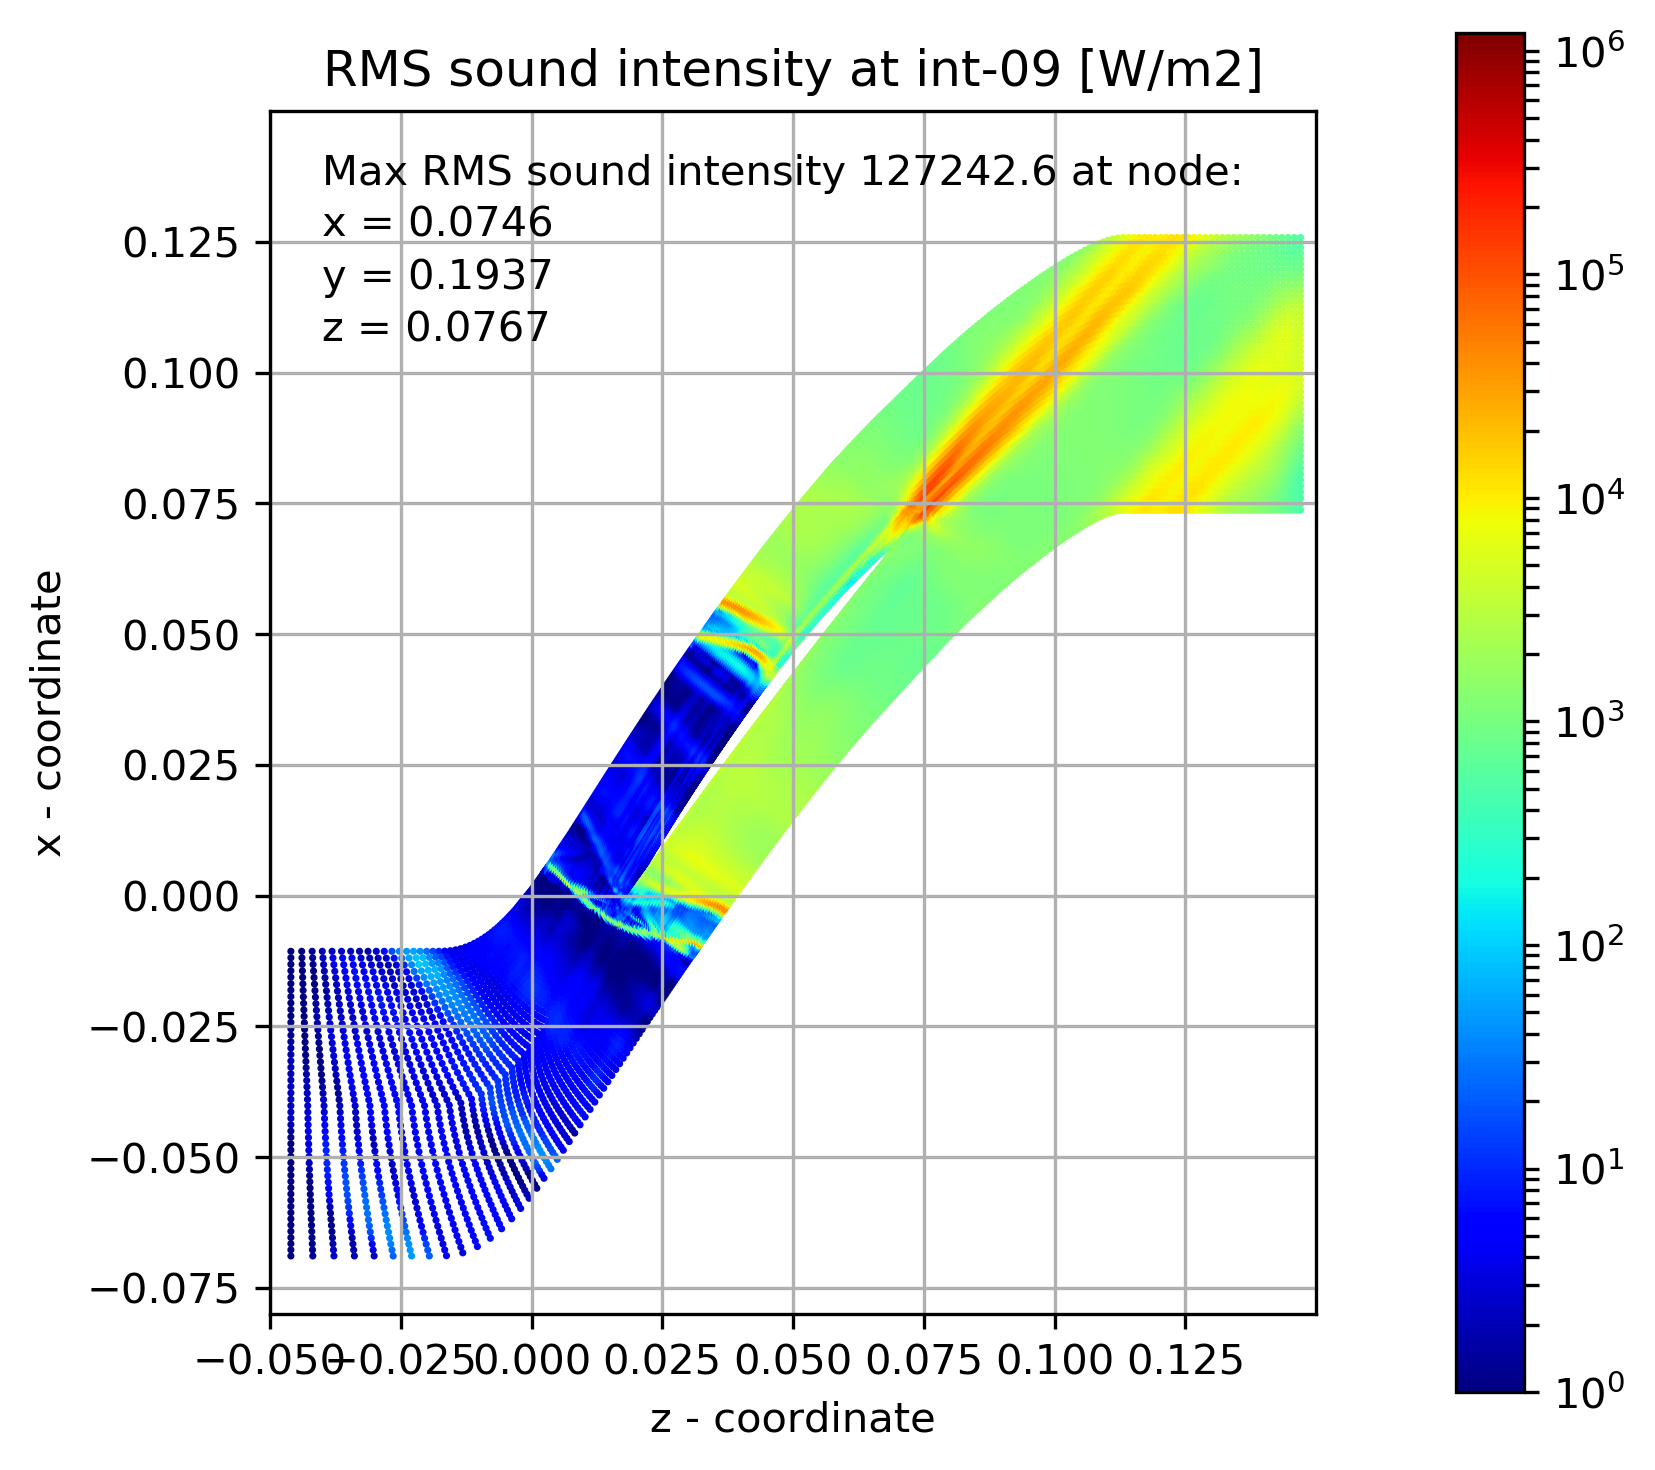
\includegraphics[width=0.75\textwidth]{Figures/int-09-rms-sil.png} \label{int-09-rms-sil}
  \caption{RMS Sound intensity at int-09 mark}
  
  \vspace*{\floatsep}% https://tex.stackexchange.com/q/26521/5764

  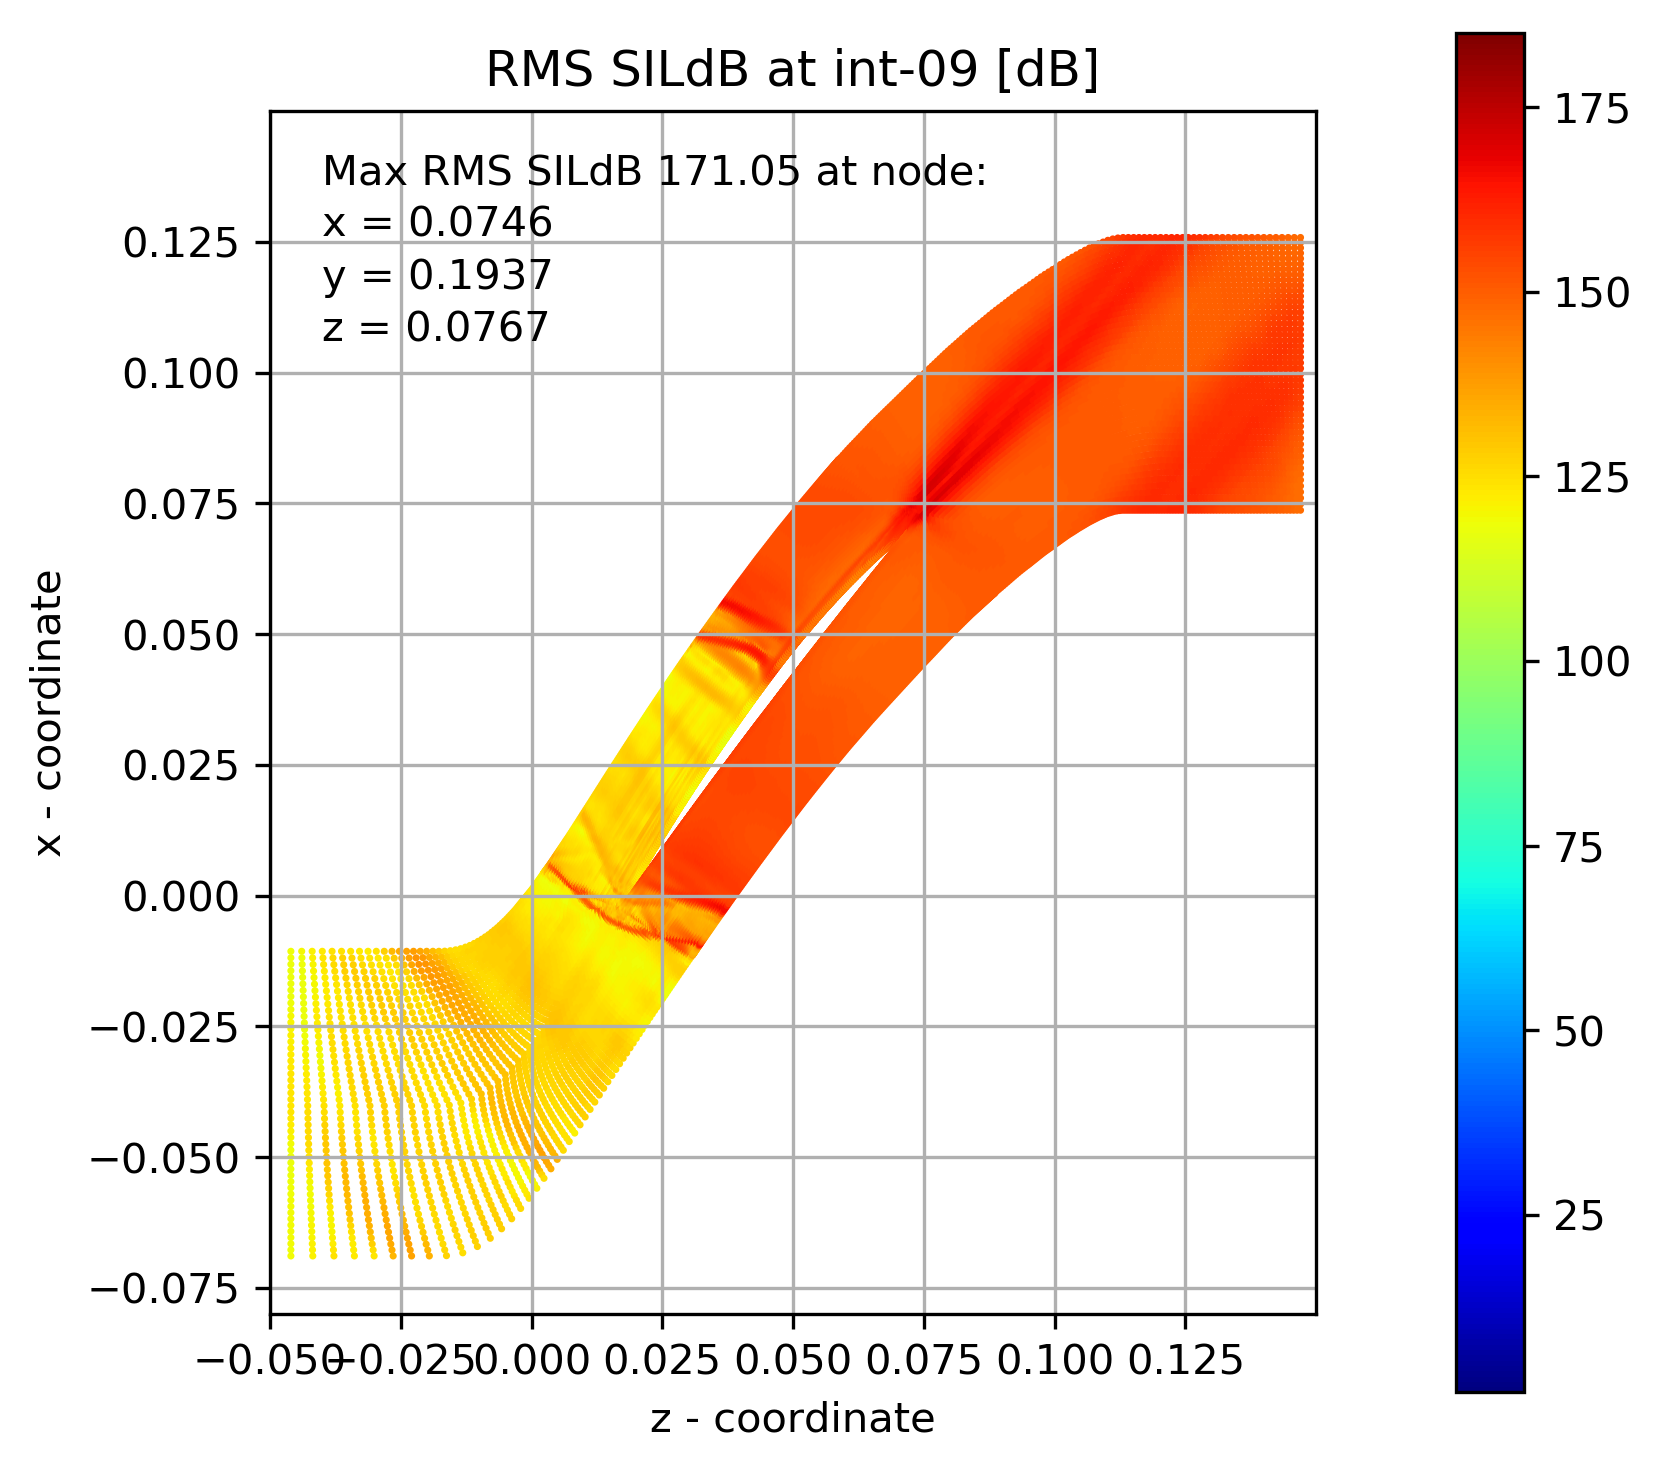
\includegraphics[width=0.75\textwidth]{Figures/int-09-rms-sildb.png} \label{int-09-rms-sildb}
  \caption{RMS Sound intensity decibel level at int-09 mark}
\end{figure}


%int-10
\begin{figure}[ht]
  \centering
  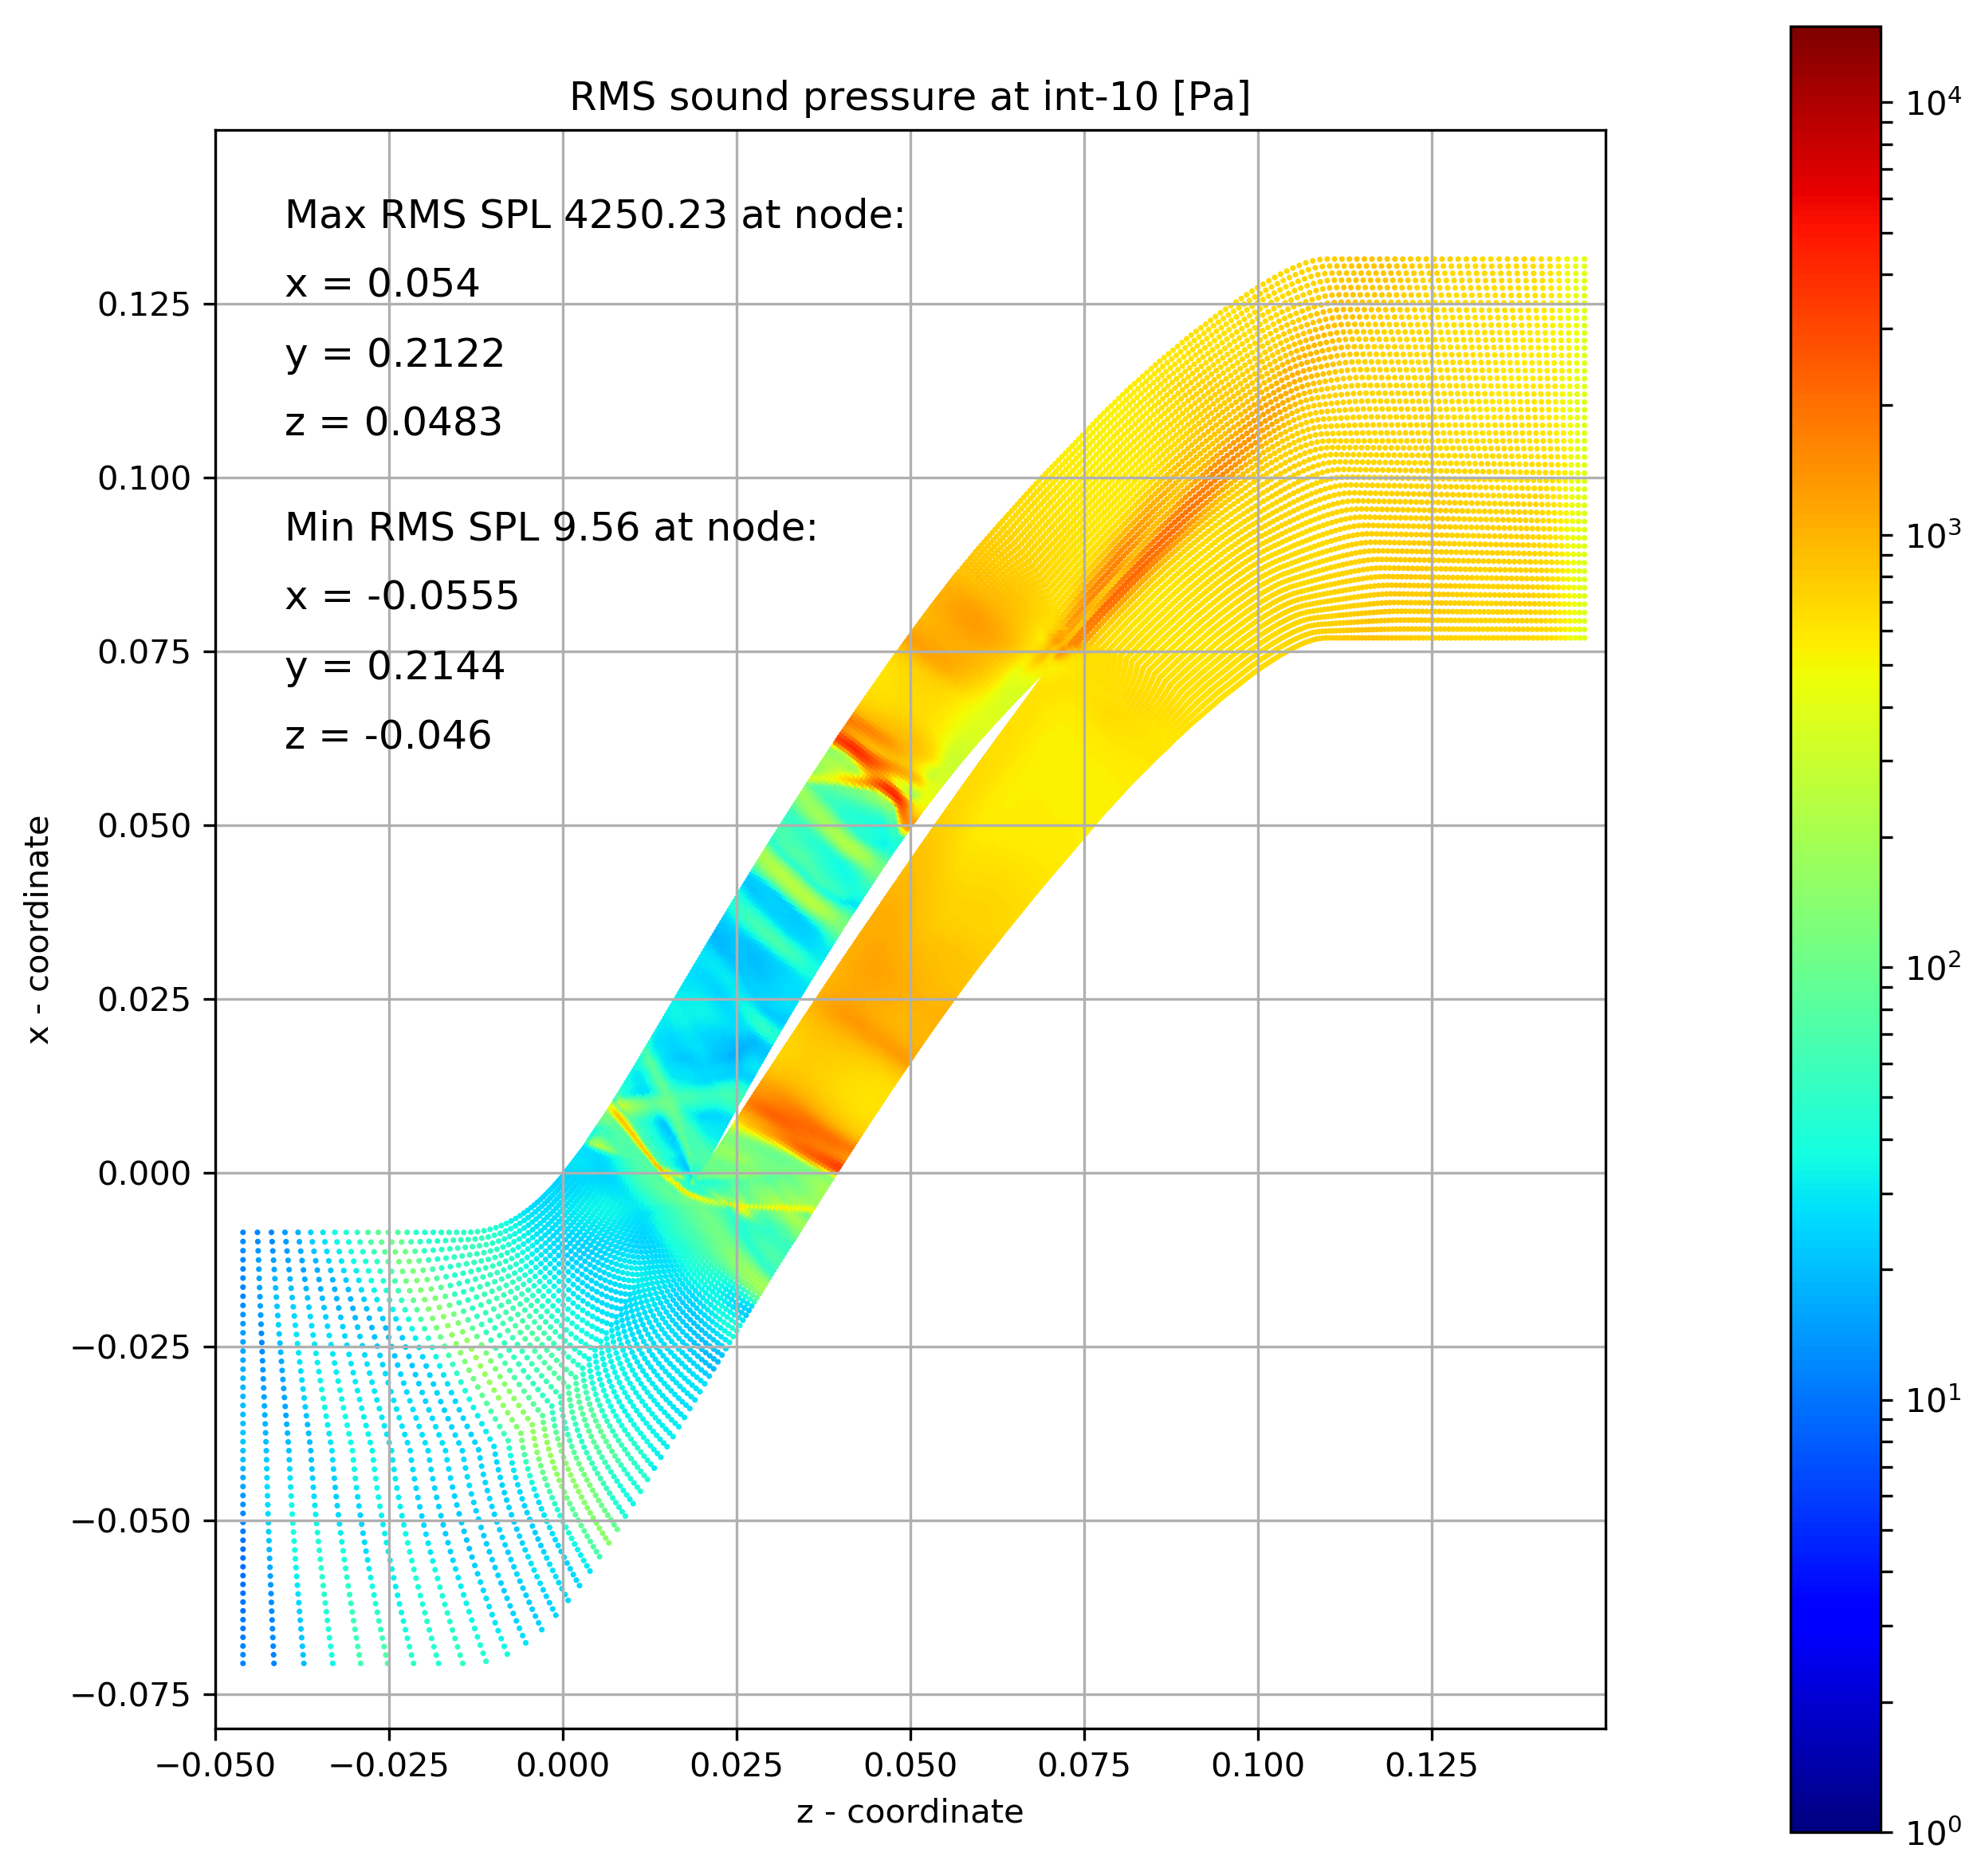
\includegraphics[width=0.75\textwidth]{Figures/int-10-rms-spl.png} \label{int-10-rms-spl}
  \caption{RMS Sound pressure at int-10 mark}
  
  \vspace*{\floatsep}% https://tex.stackexchange.com/q/26521/5764

  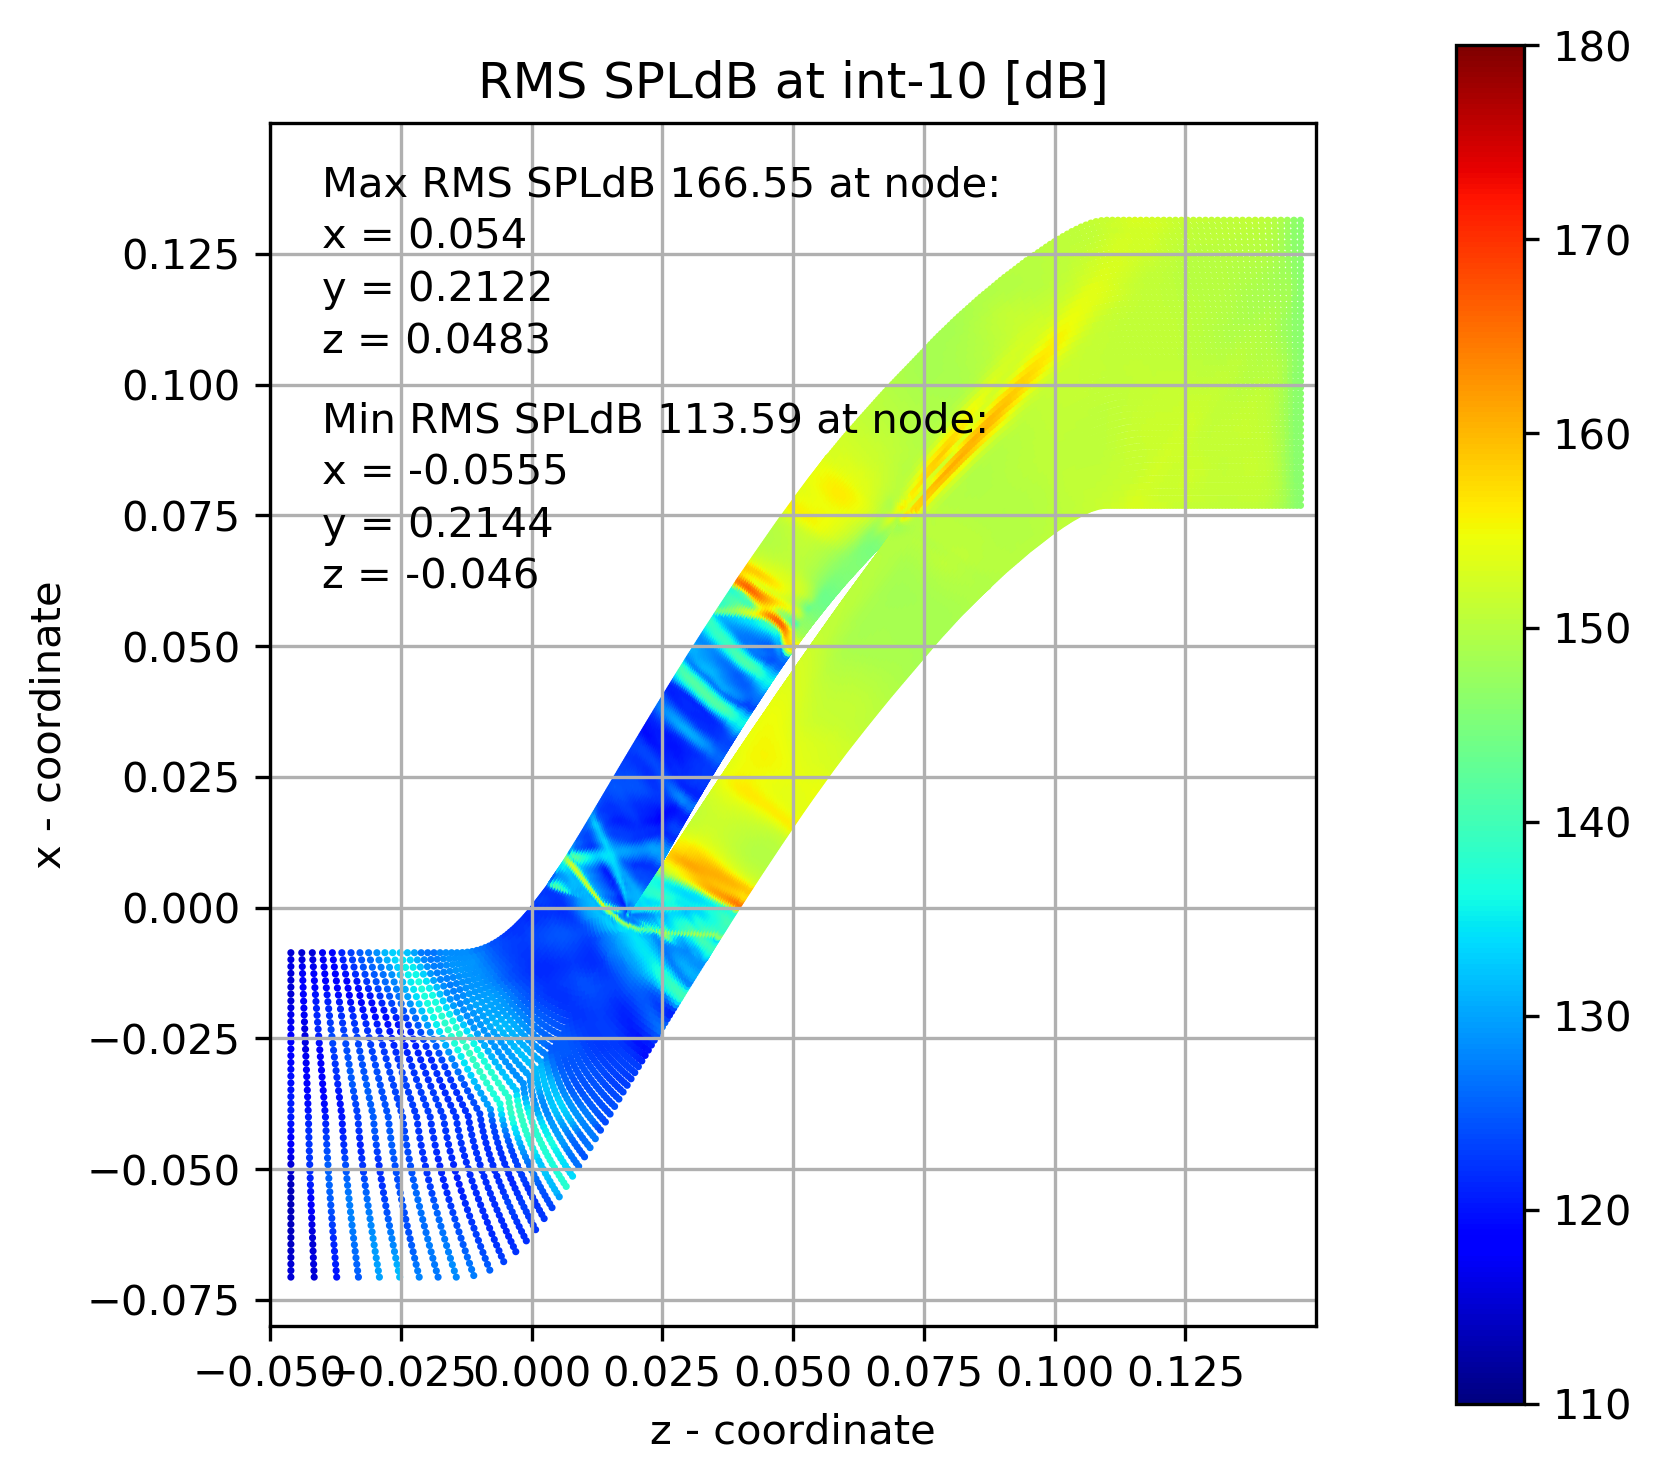
\includegraphics[width=0.75\textwidth]{Figures/int-10-rms-spldb.png} \label{int-10-rms-spldb}
  \caption{RMS Sound pressure decibel level at int-10 mark}
\end{figure}
%int-10
\begin{figure}[ht]
  \centering
  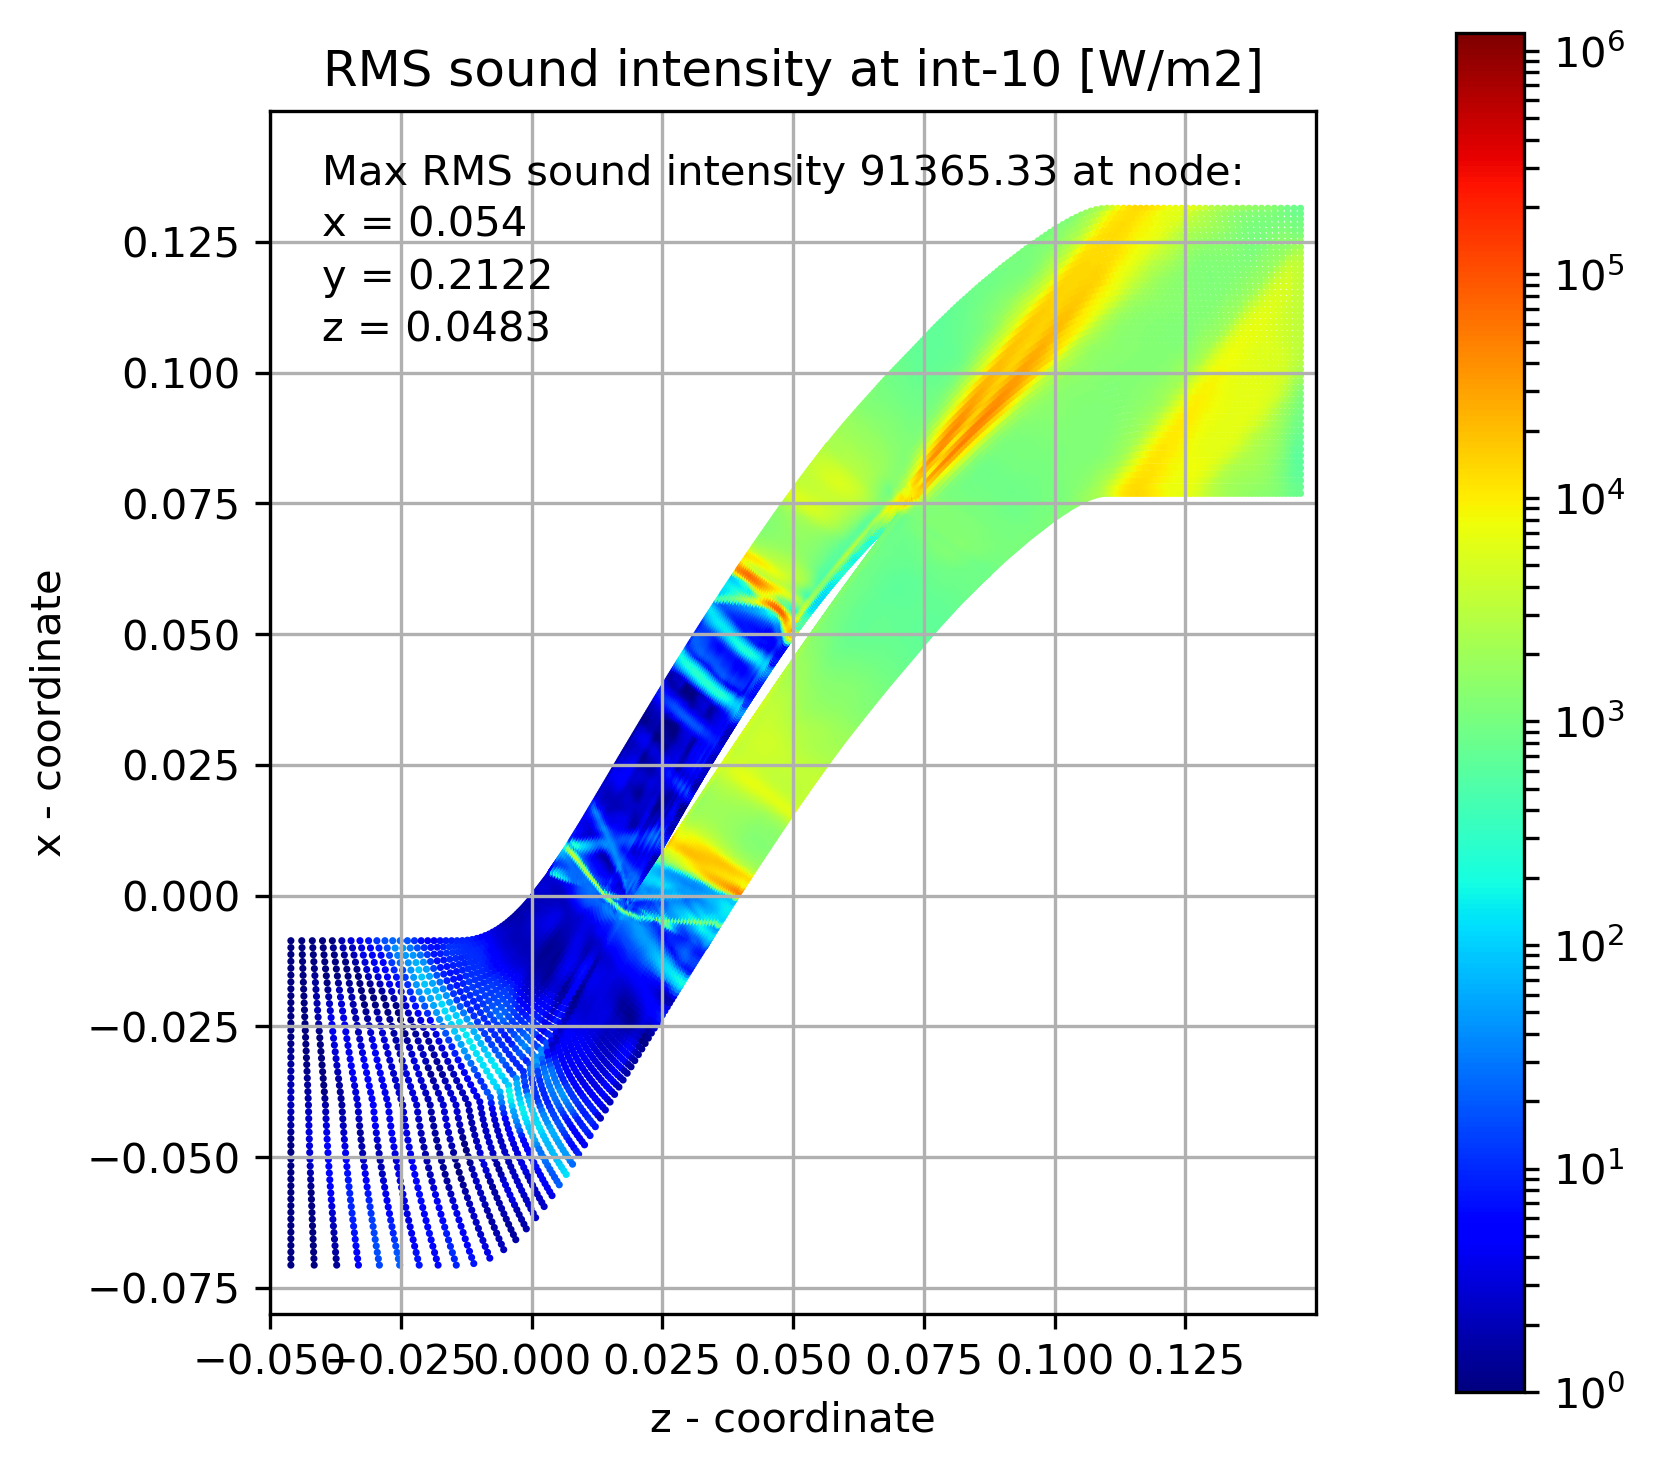
\includegraphics[width=0.75\textwidth]{Figures/int-10-rms-sil.png} \label{int-10-rms-sil}
  \caption{RMS Sound intensity at int-10 mark}
  
  \vspace*{\floatsep}% https://tex.stackexchange.com/q/26521/5764

  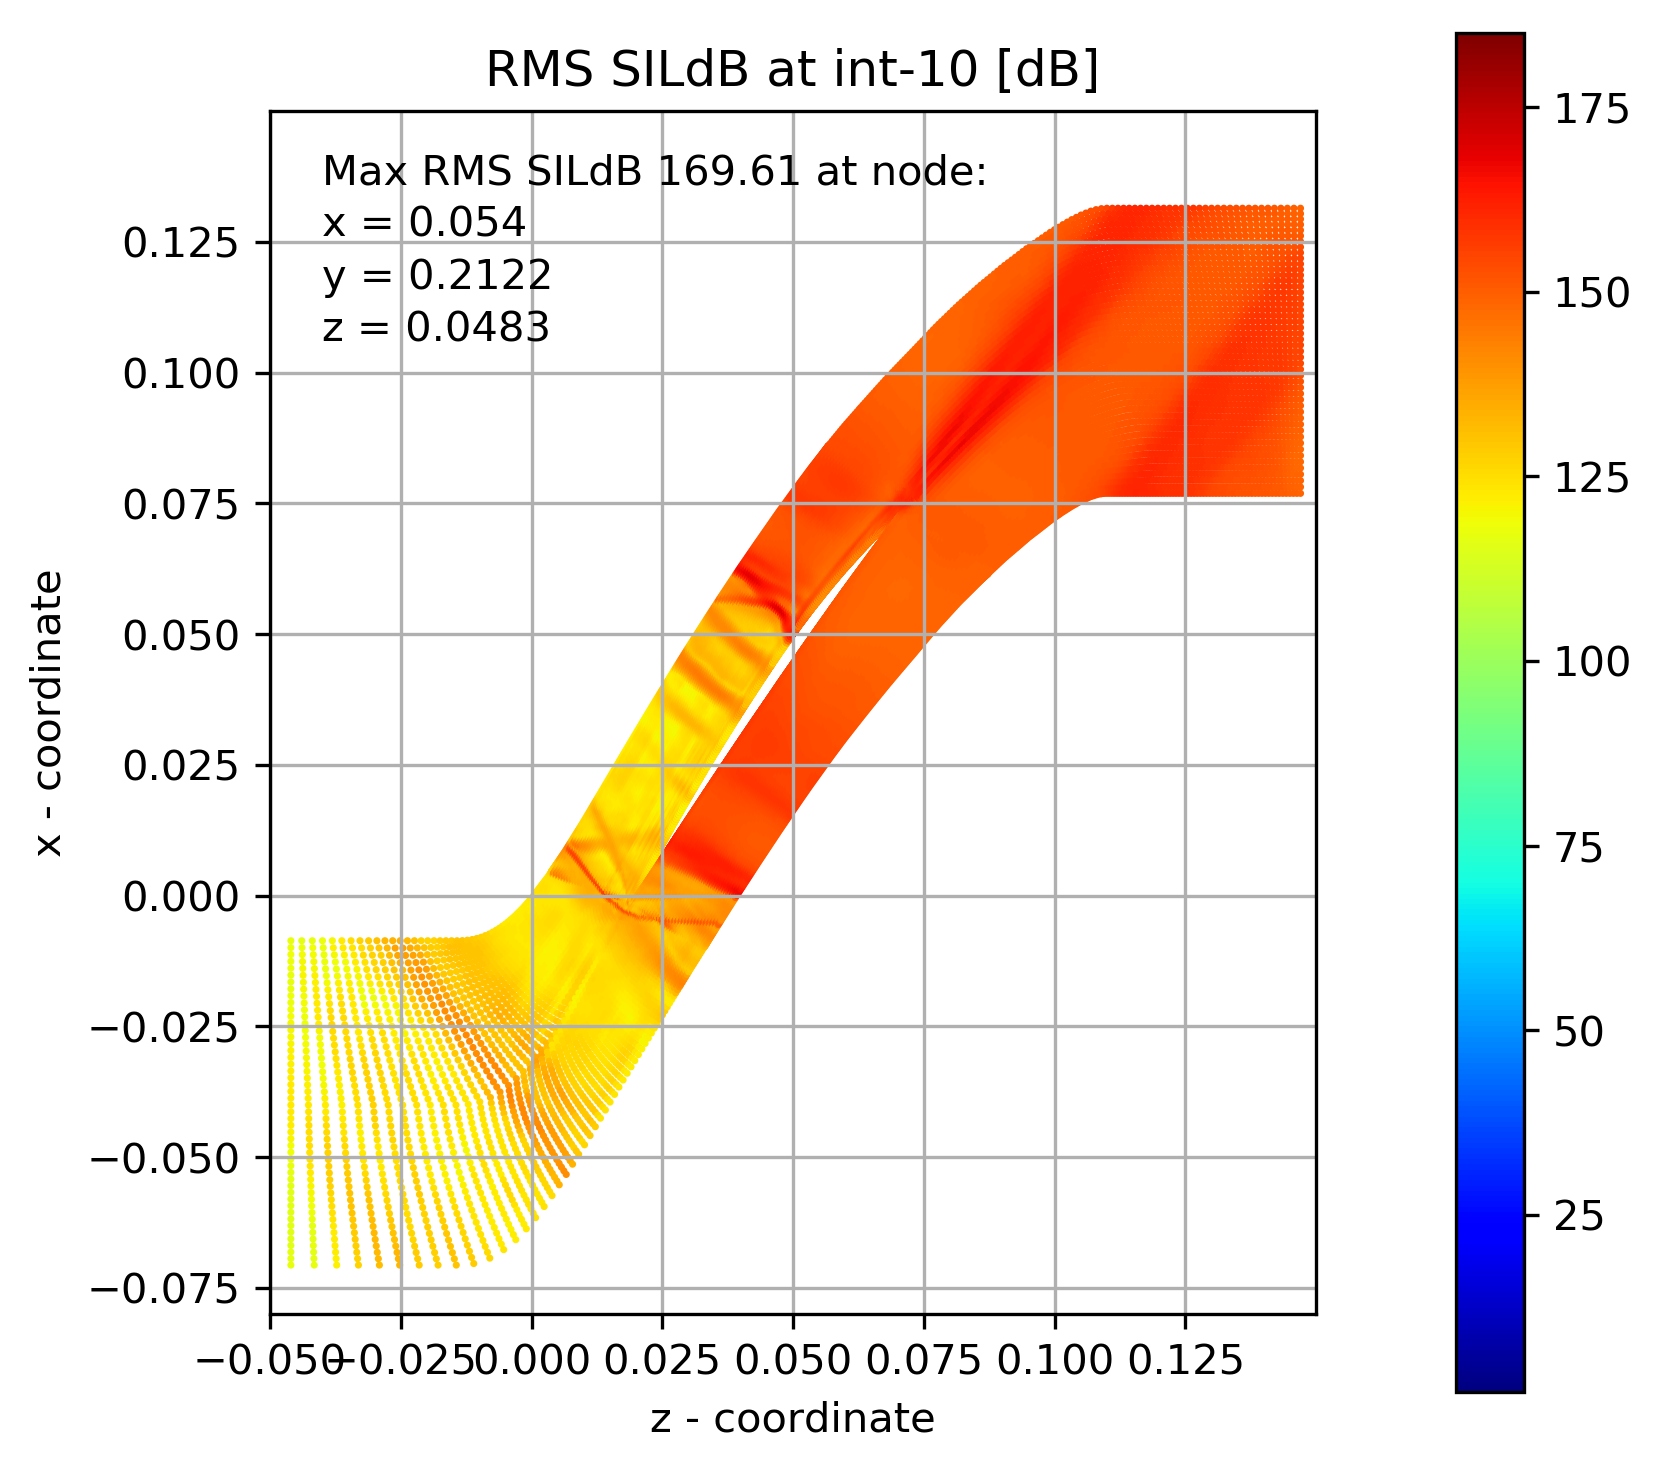
\includegraphics[width=0.75\textwidth]{Figures/int-10-rms-sildb.png} \label{int-10-rms-sildb}
  \caption{RMS Sound intensity decibel level at int-10 mark}
\end{figure}


%int-11
\begin{figure}[ht]
  \centering
  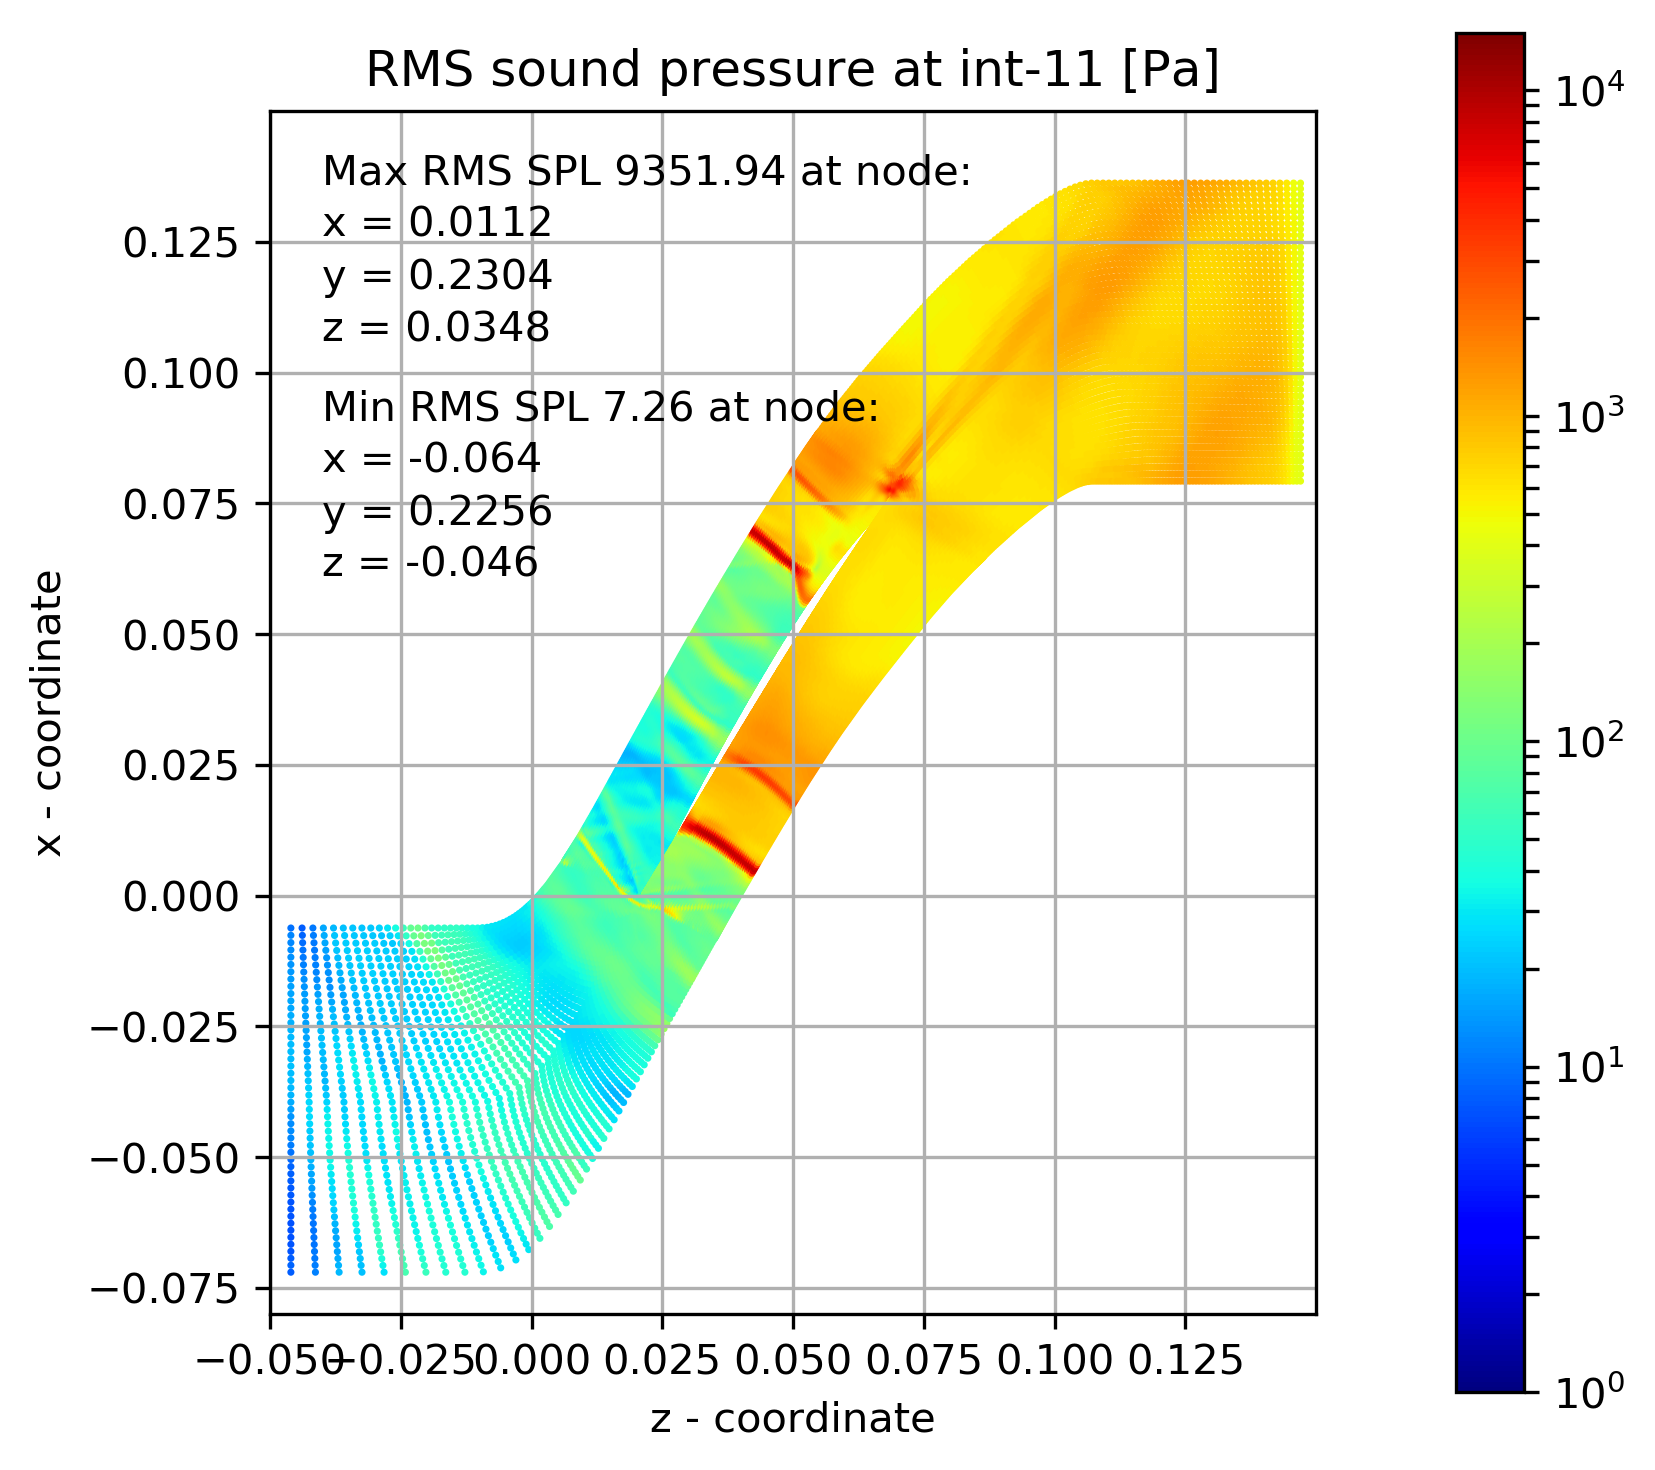
\includegraphics[width=0.75\textwidth]{Figures/int-11-rms-spl.png} \label{int-11-rms-spl}
  \caption{RMS Sound pressure at int-11 mark}
  
  \vspace*{\floatsep}% https://tex.stackexchange.com/q/26521/5764

  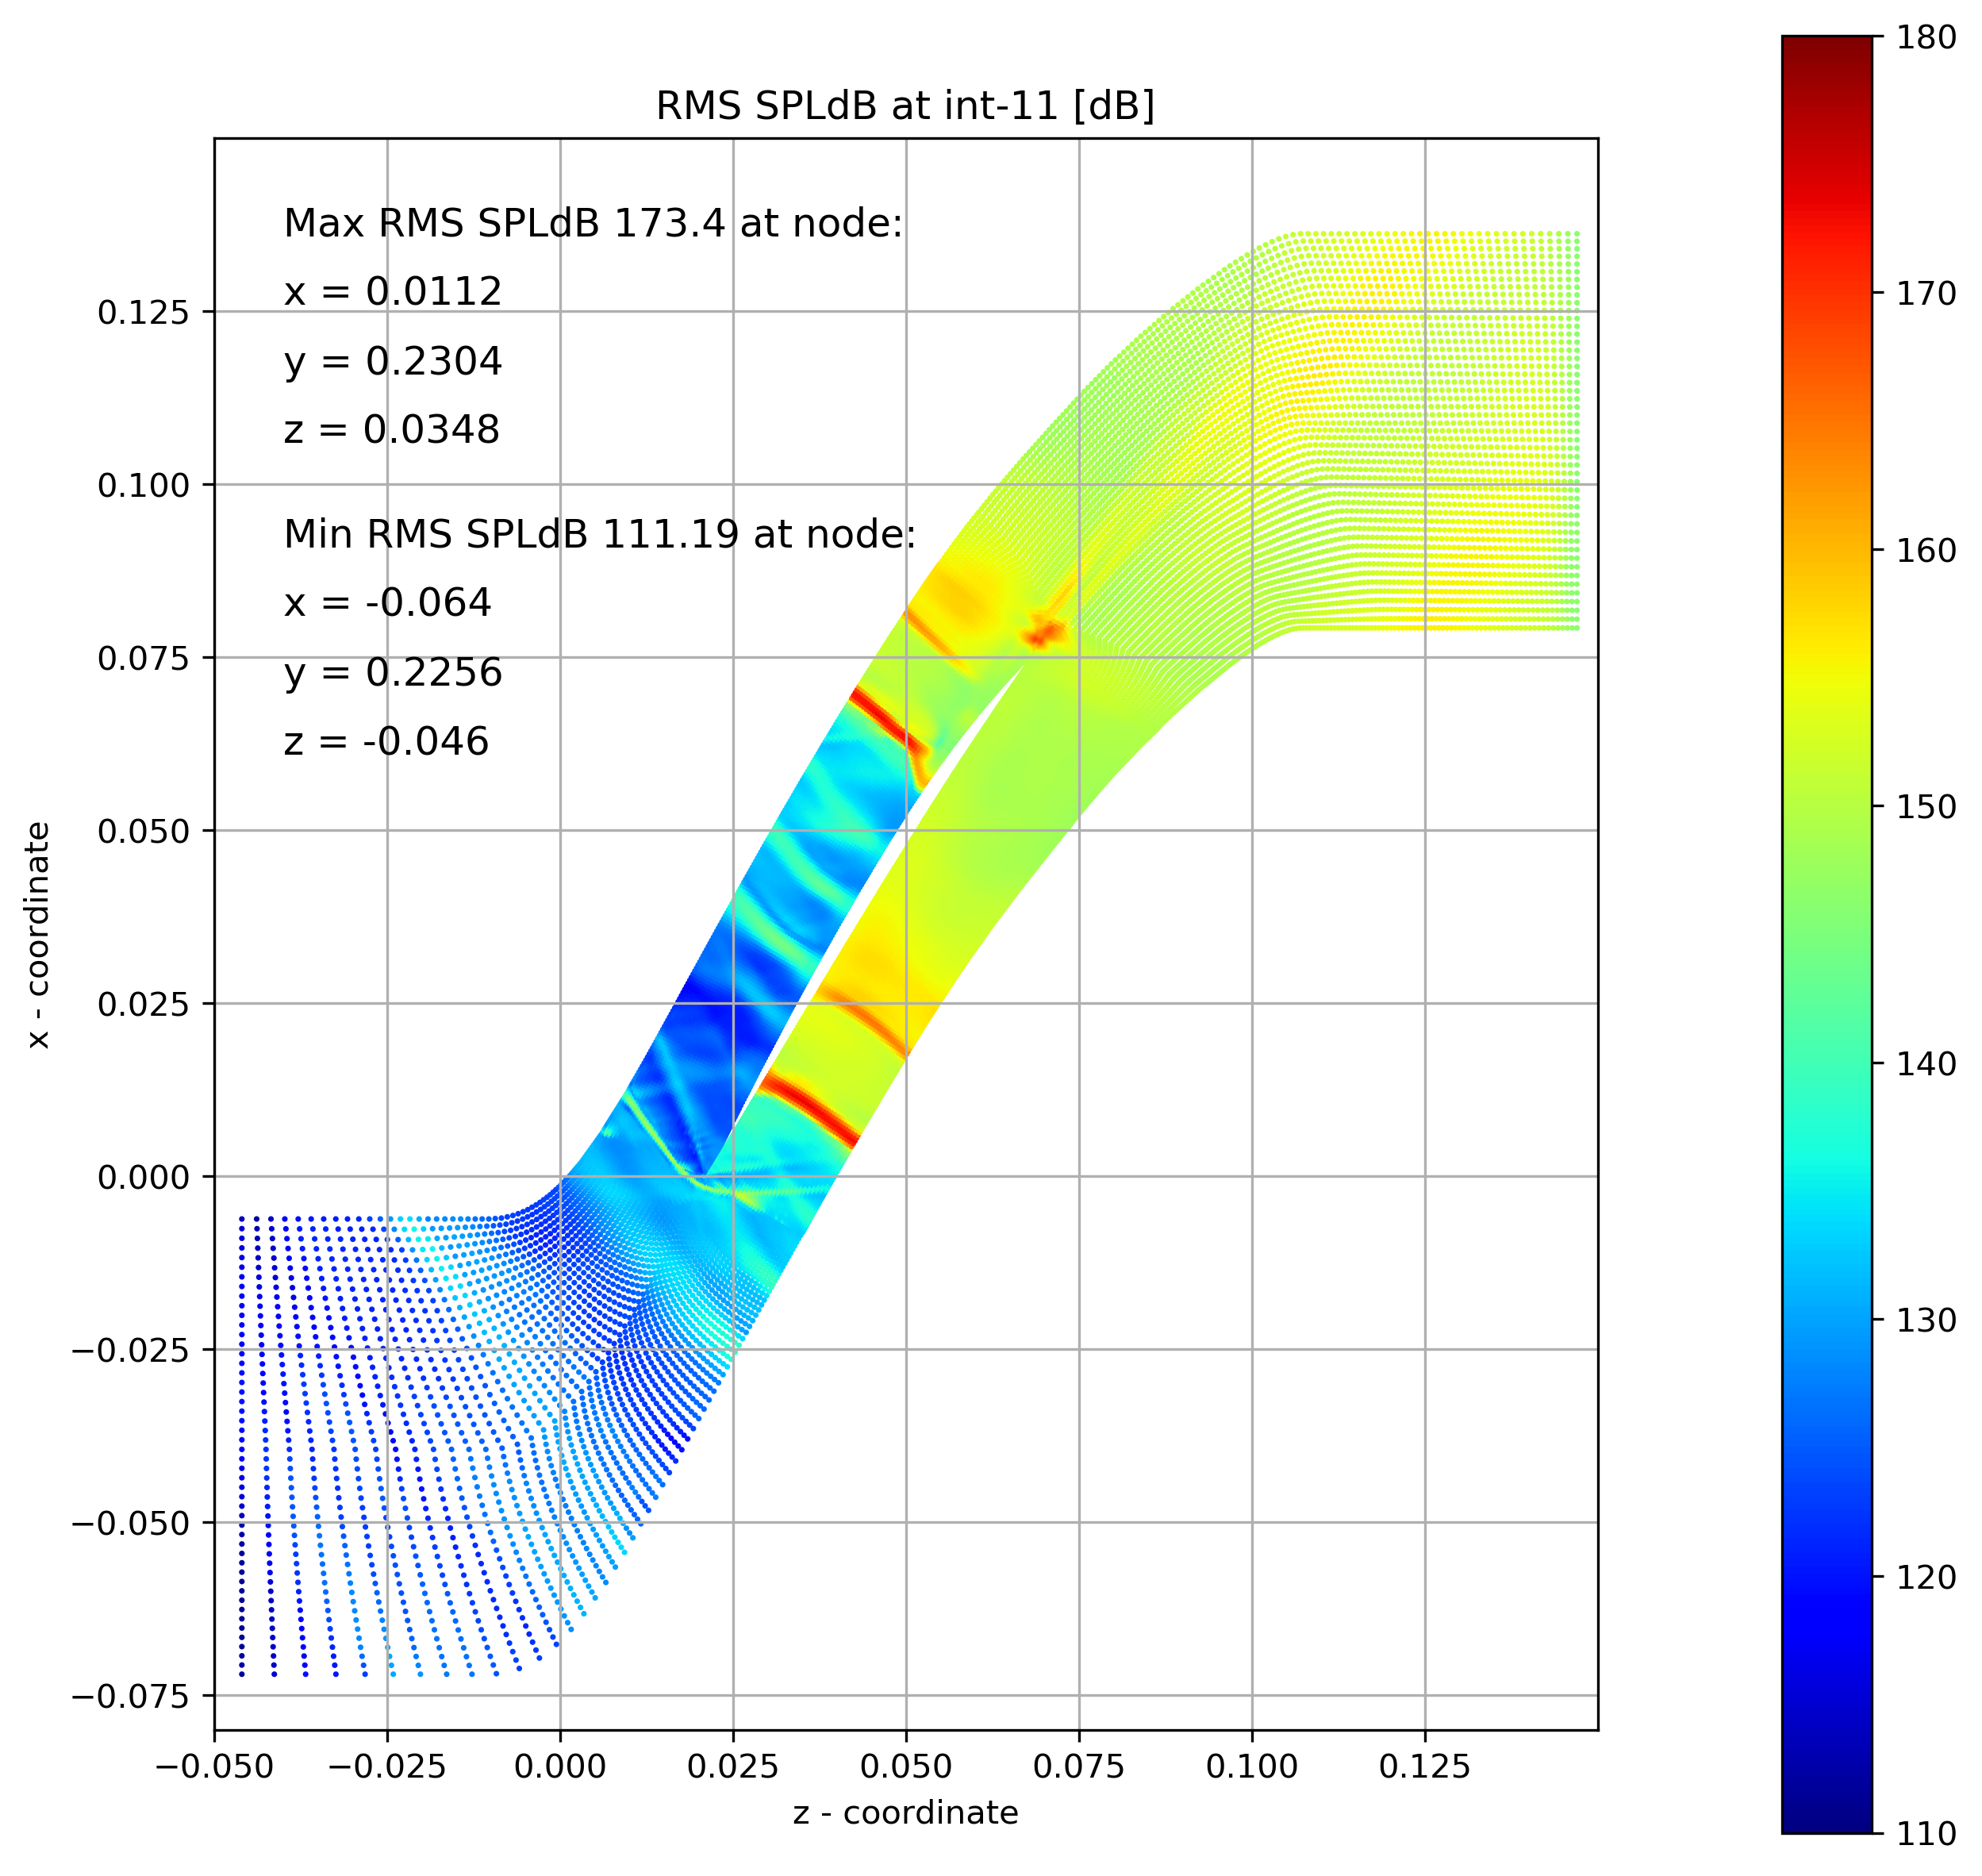
\includegraphics[width=0.75\textwidth]{Figures/int-11-rms-spldb.png} \label{int-11-rms-spldb}
  \caption{RMS Sound pressure decibel level at int-11 mark}
\end{figure}
%int-11
\begin{figure}[ht]
  \centering
  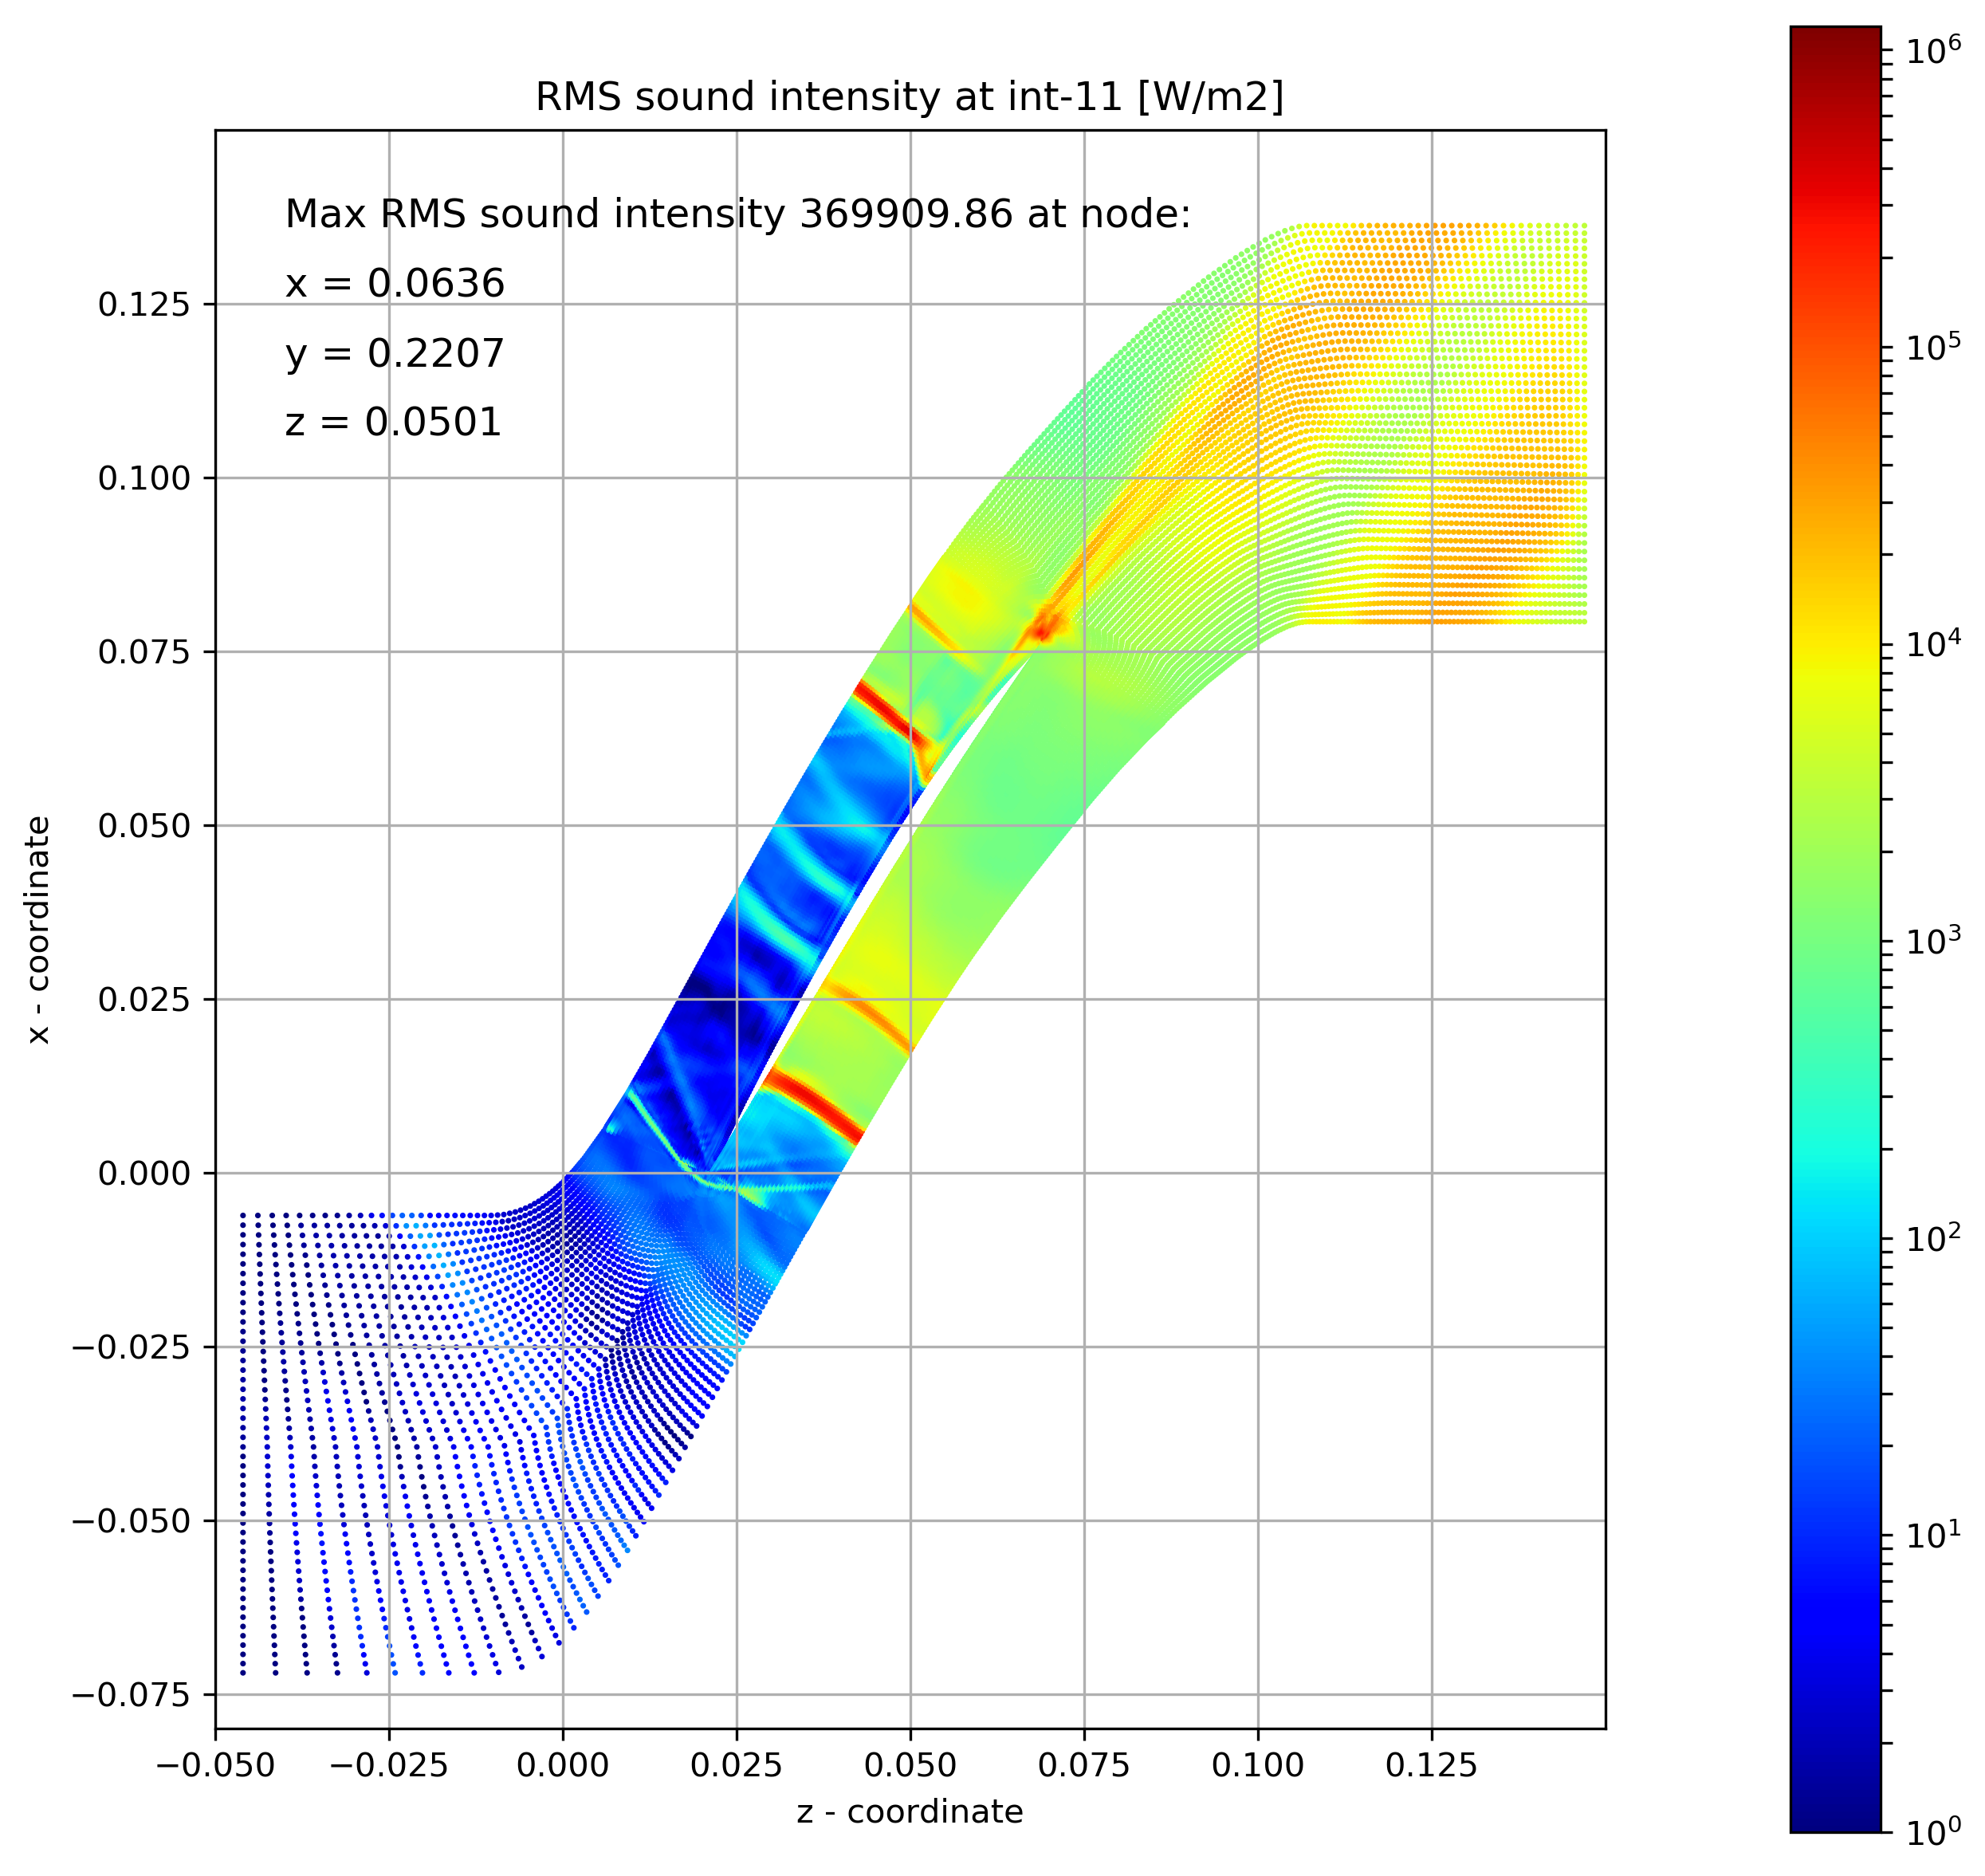
\includegraphics[width=0.75\textwidth]{Figures/int-11-rms-sil.png} \label{int-11-rms-sil}
  \caption{RMS Sound intensity at int-11 mark}
  
  \vspace*{\floatsep}% https://tex.stackexchange.com/q/26521/5764

  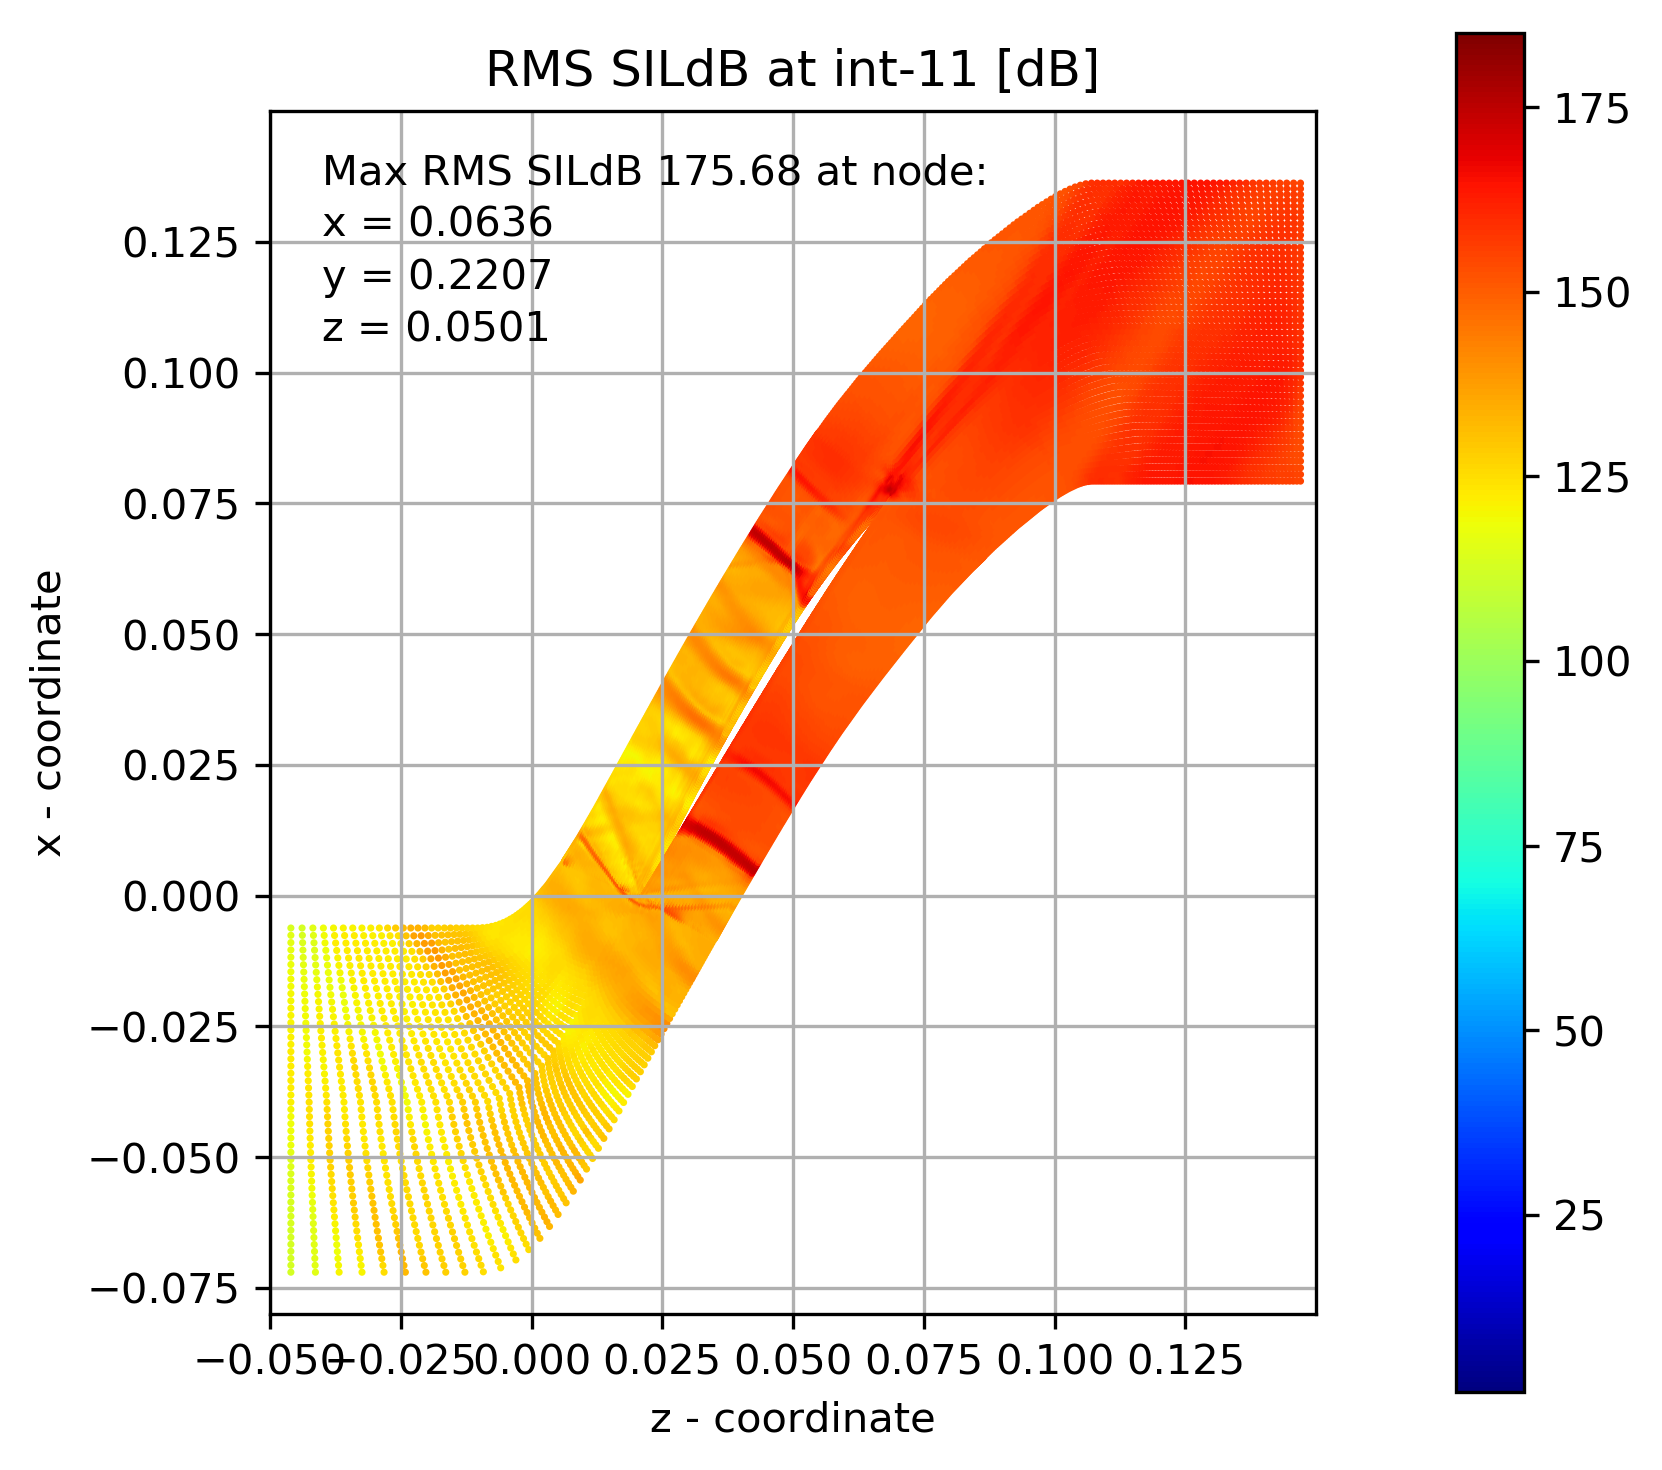
\includegraphics[width=0.75\textwidth]{Figures/int-11-rms-sildb.png} \label{int-11-rms-sildb}
  \caption{RMS Sound intensity decibel level at int-11 mark}
\end{figure}


%int-12
\begin{figure}[ht]
  \centering
  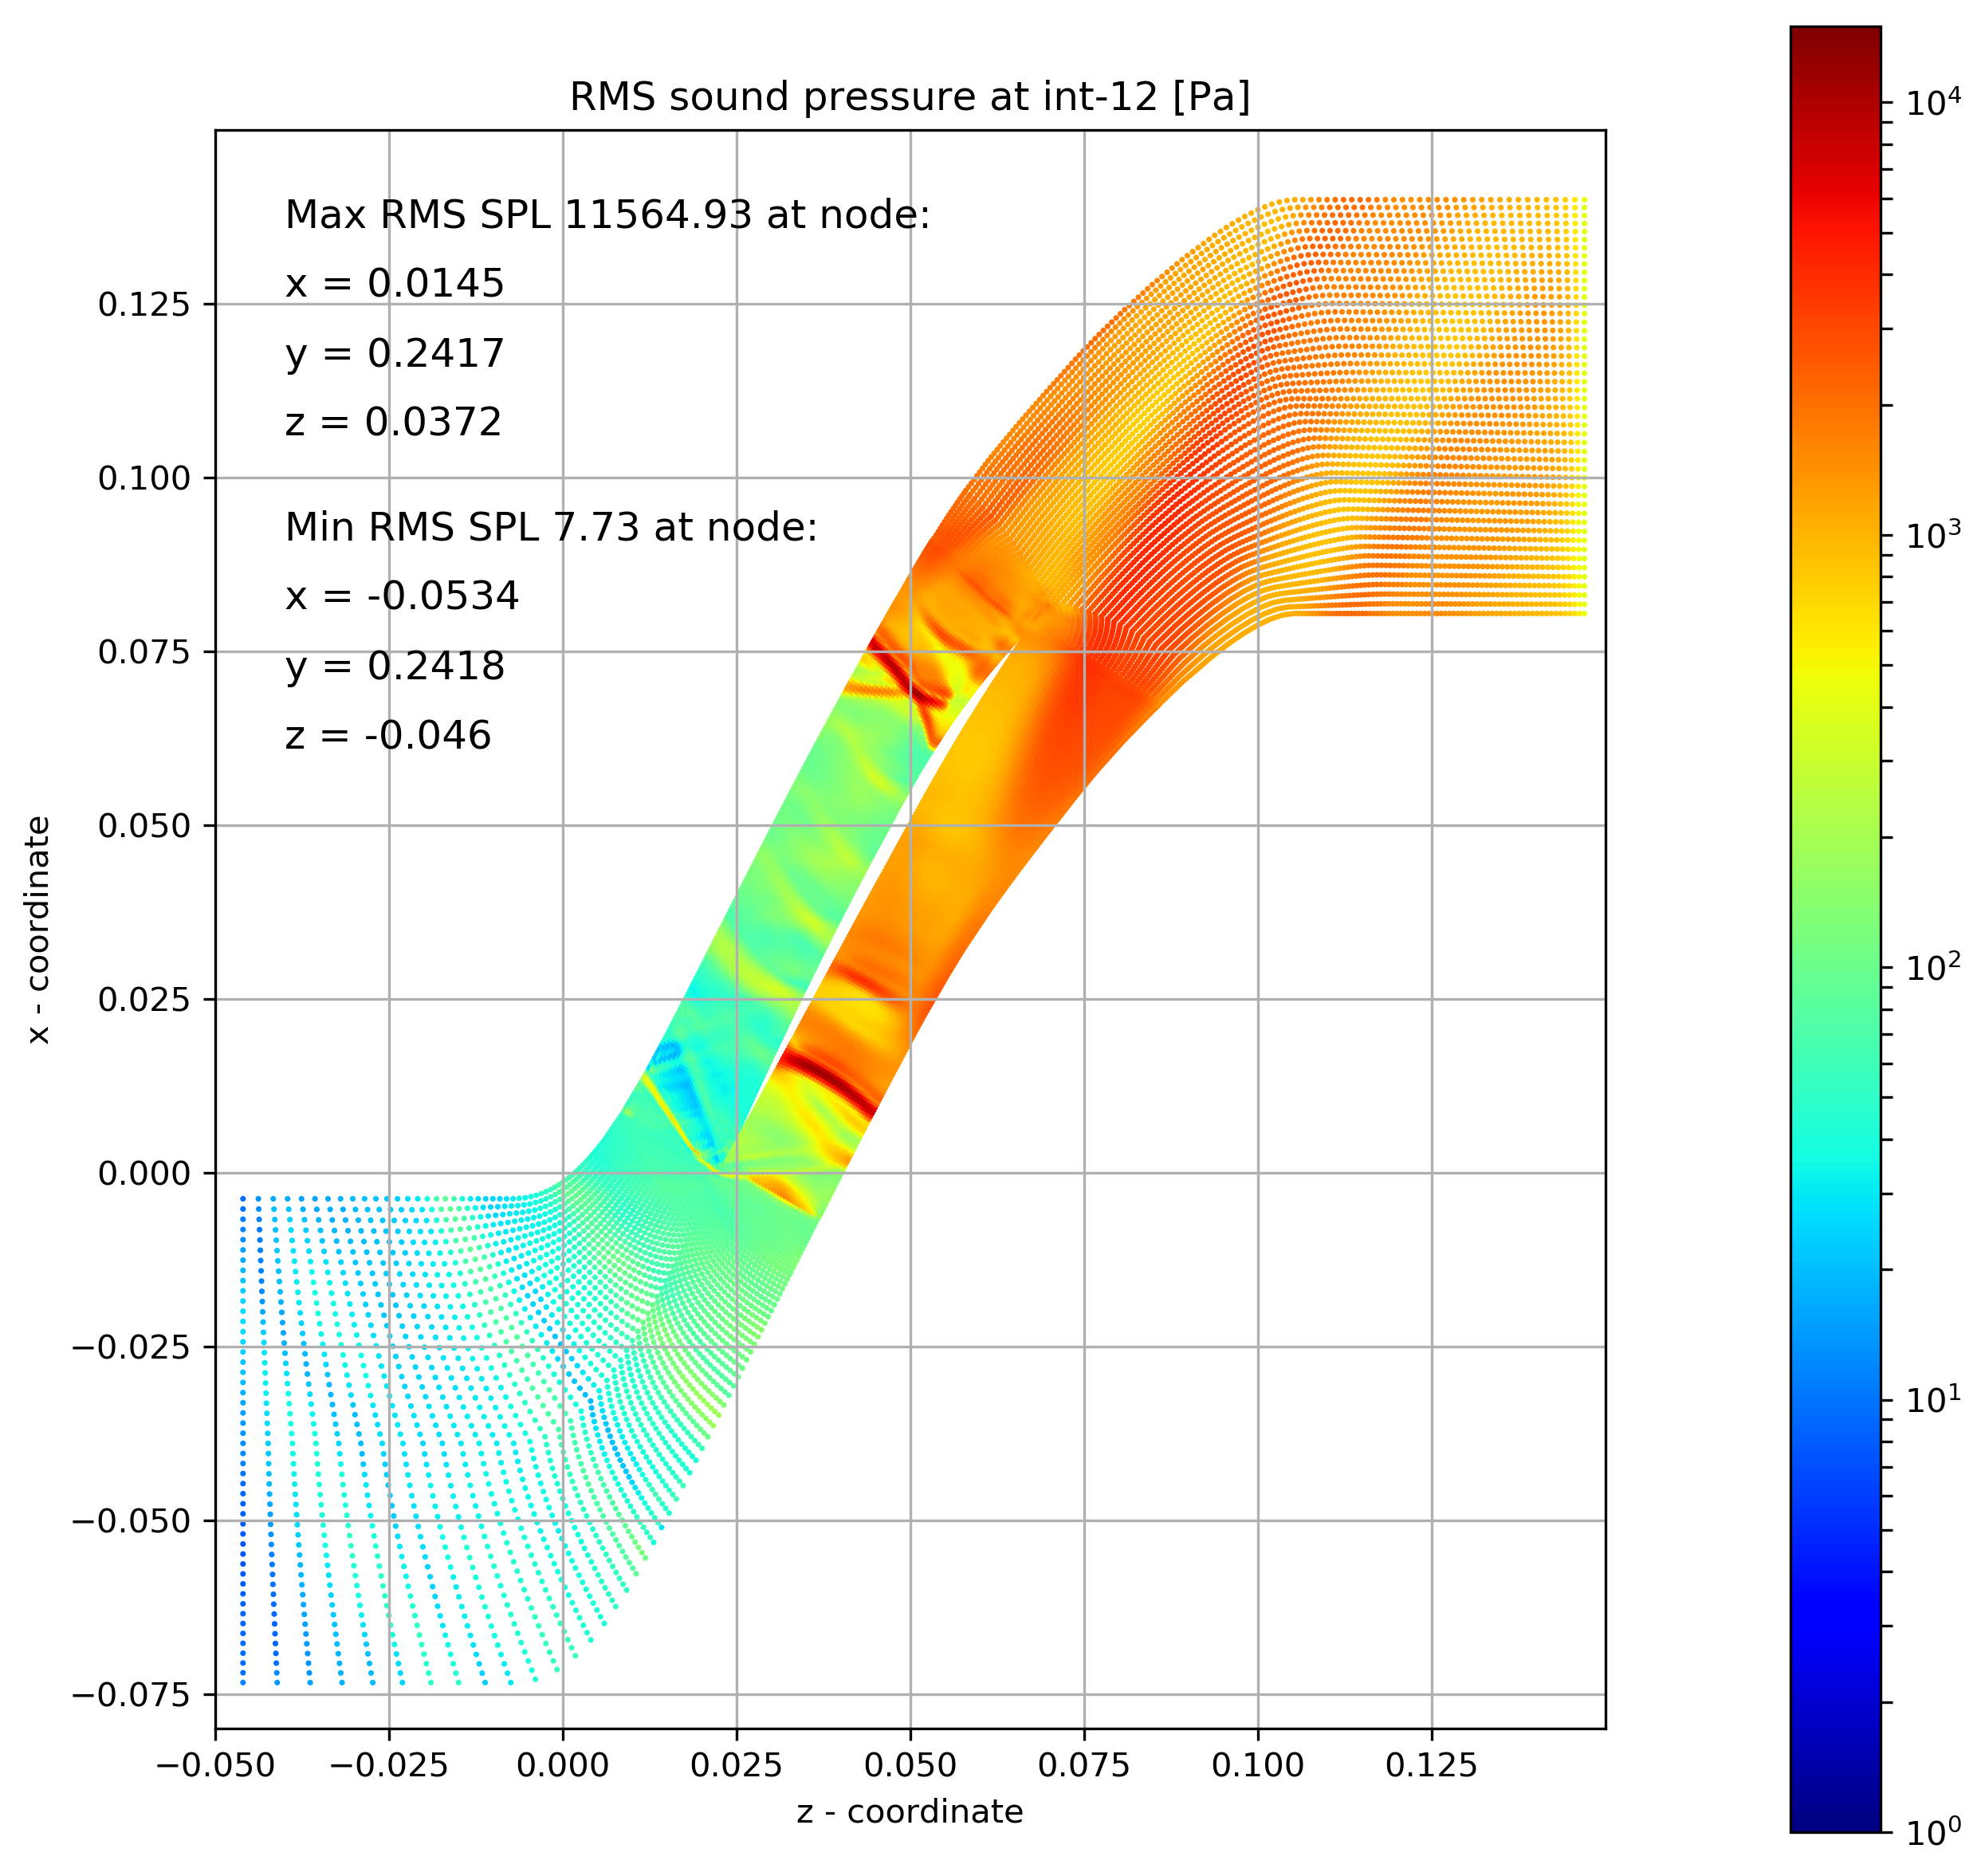
\includegraphics[width=0.75\textwidth]{Figures/int-12-rms-spl.png} \label{int-12-rms-spl}
  \caption{RMS Sound pressure at int-12 mark}
  
  \vspace*{\floatsep}% https://tex.stackexchange.com/q/26521/5764

  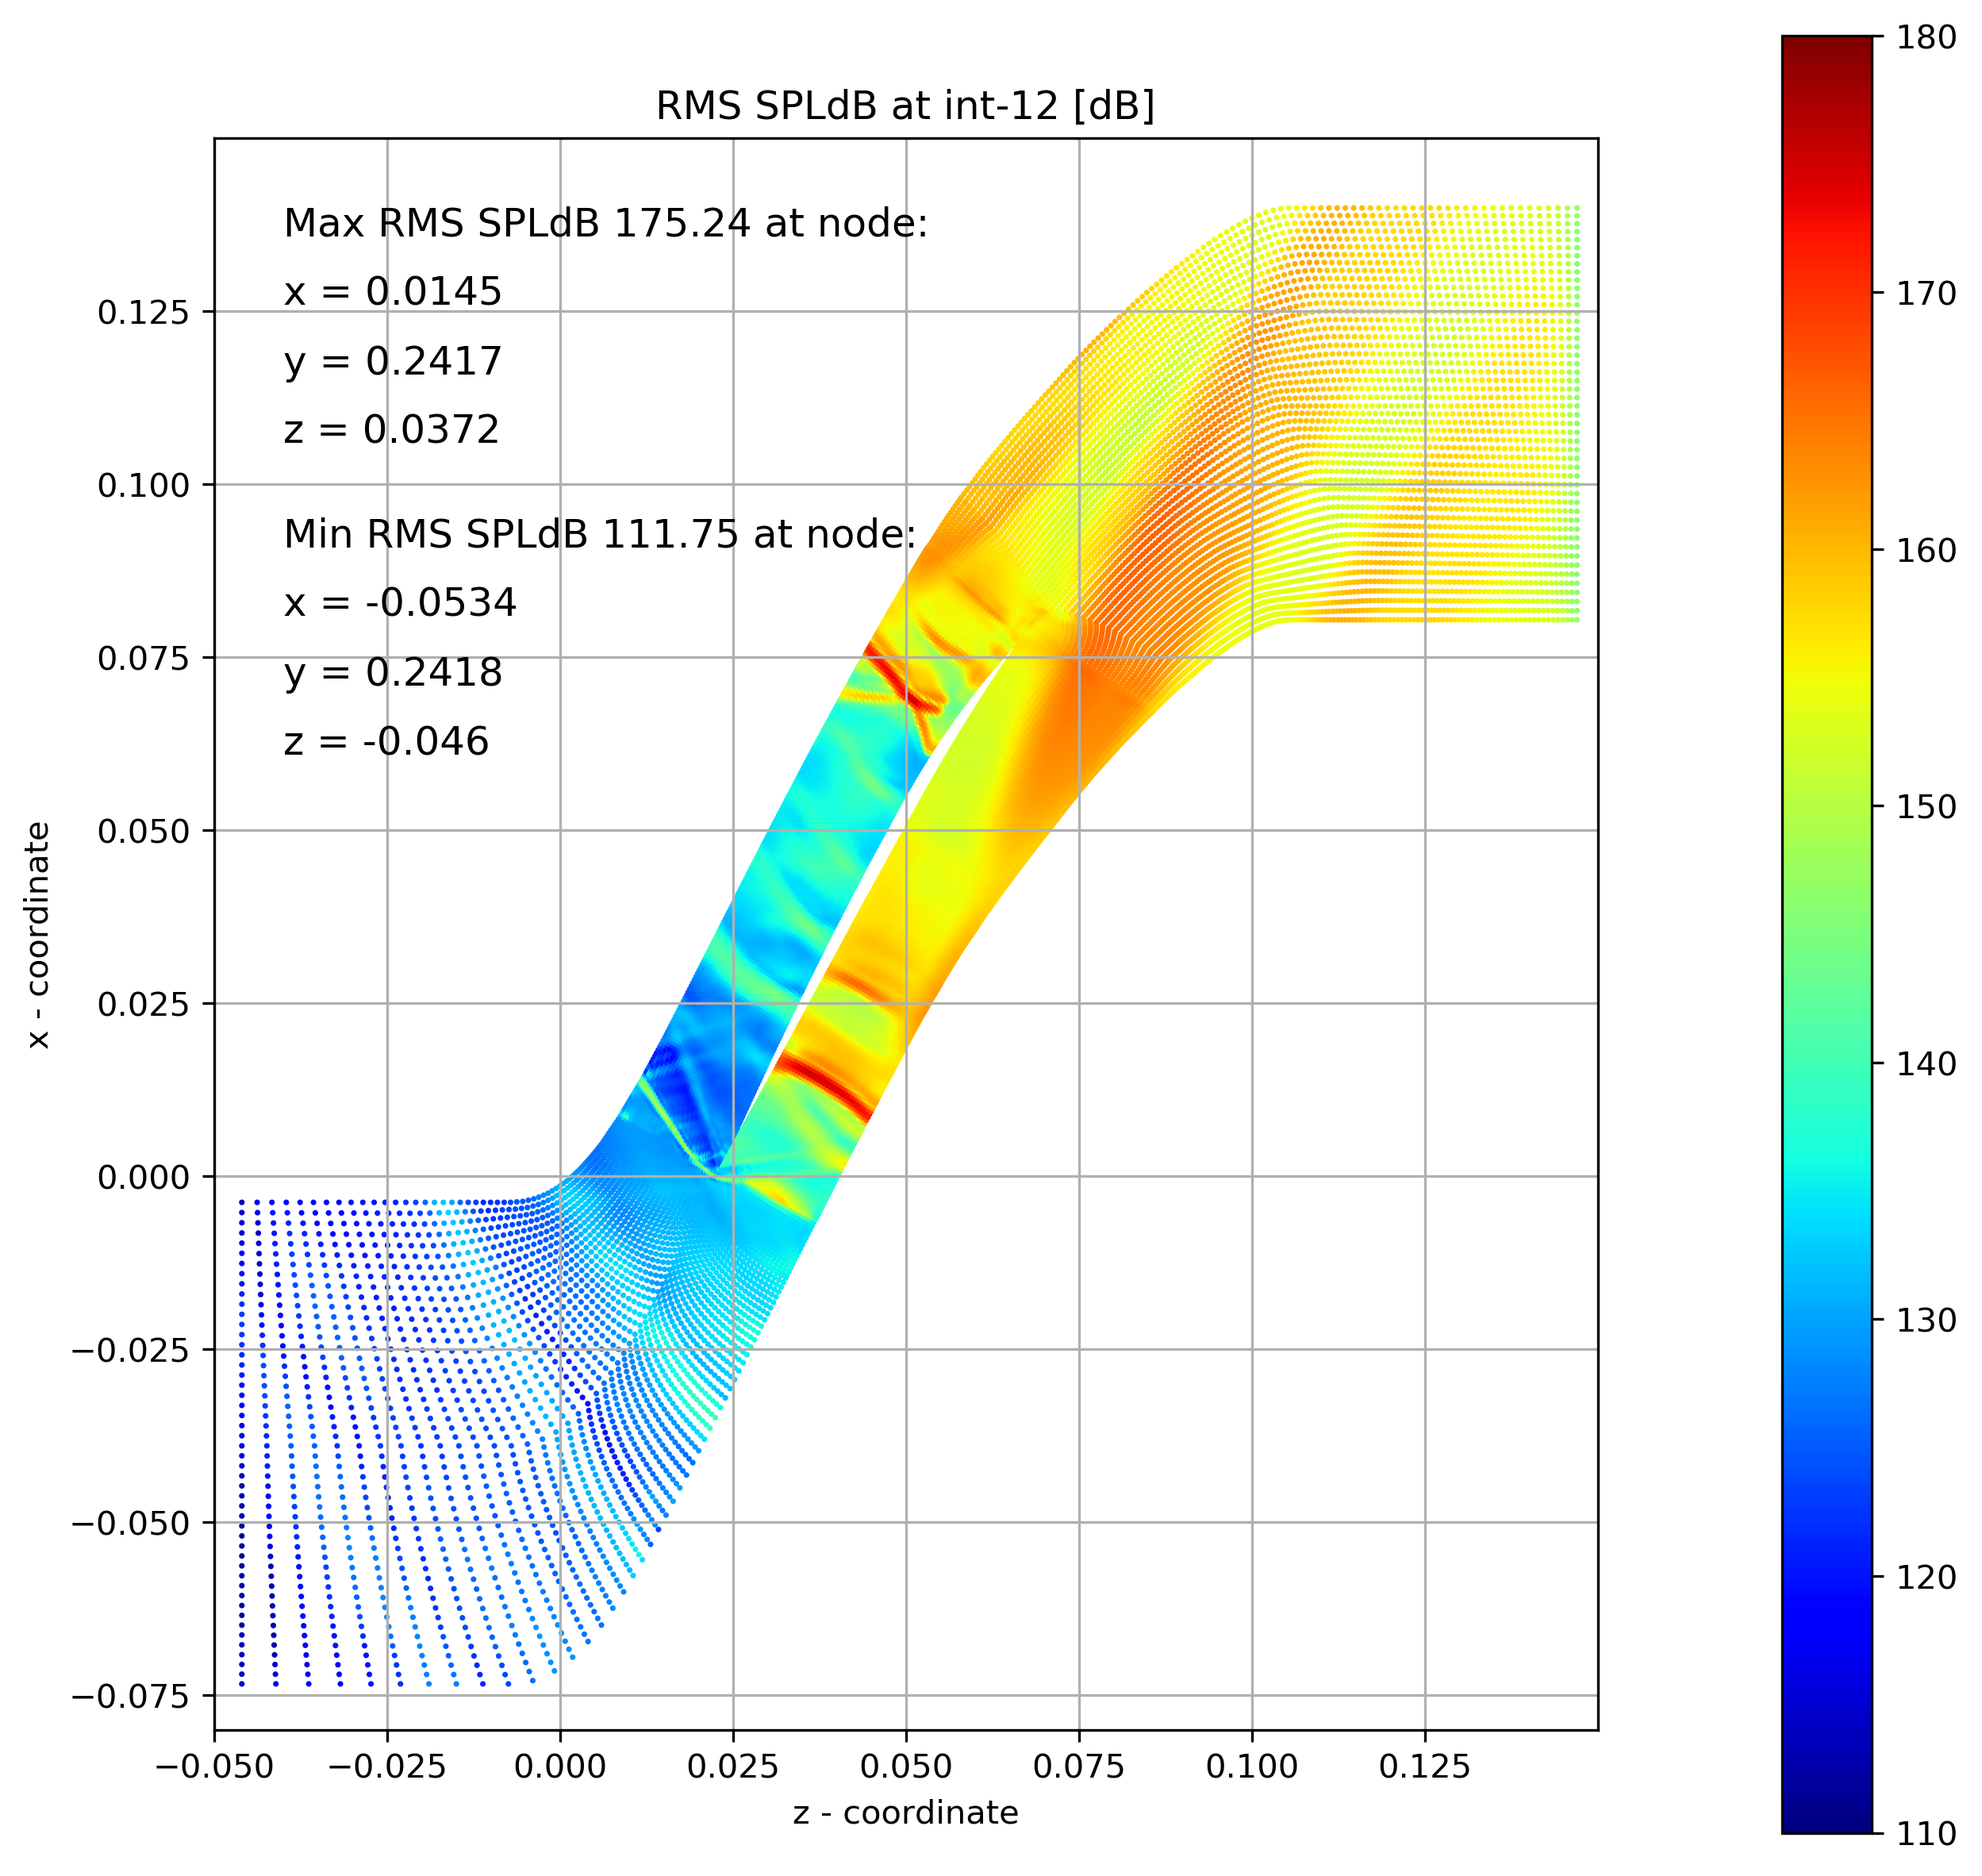
\includegraphics[width=0.75\textwidth]{Figures/int-12-rms-spldb.png} \label{int-12-rms-spldb}
  \caption{RMS Sound pressure decibel level at int-12 mark}
\end{figure}
%int-12
\begin{figure}[ht]
  \centering
  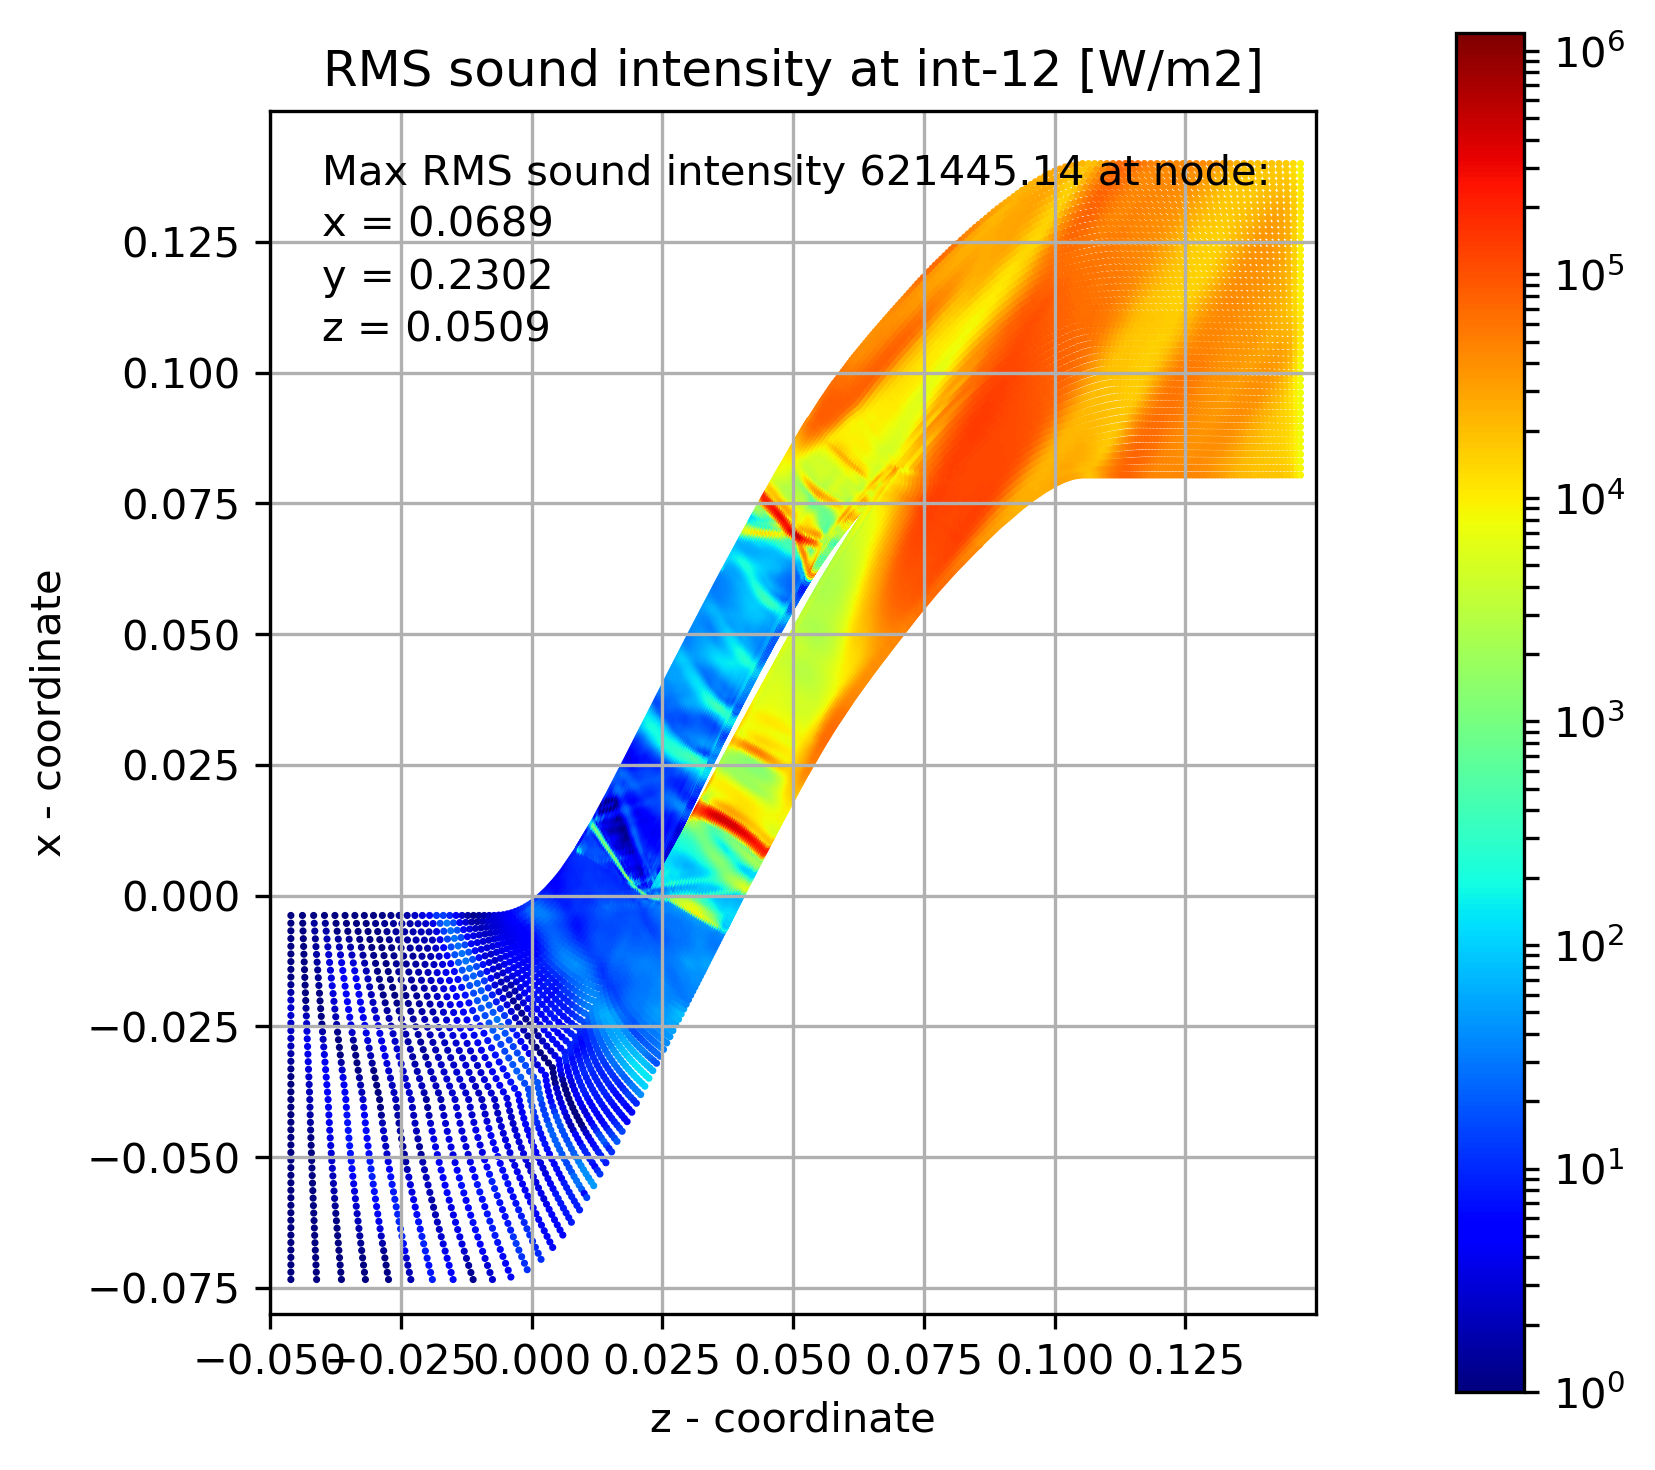
\includegraphics[width=0.75\textwidth]{Figures/int-12-rms-sil.png} \label{int-12-rms-sil}
  \caption{RMS Sound intensity at int-12 mark}
  
  \vspace*{\floatsep}% https://tex.stackexchange.com/q/26521/5764

  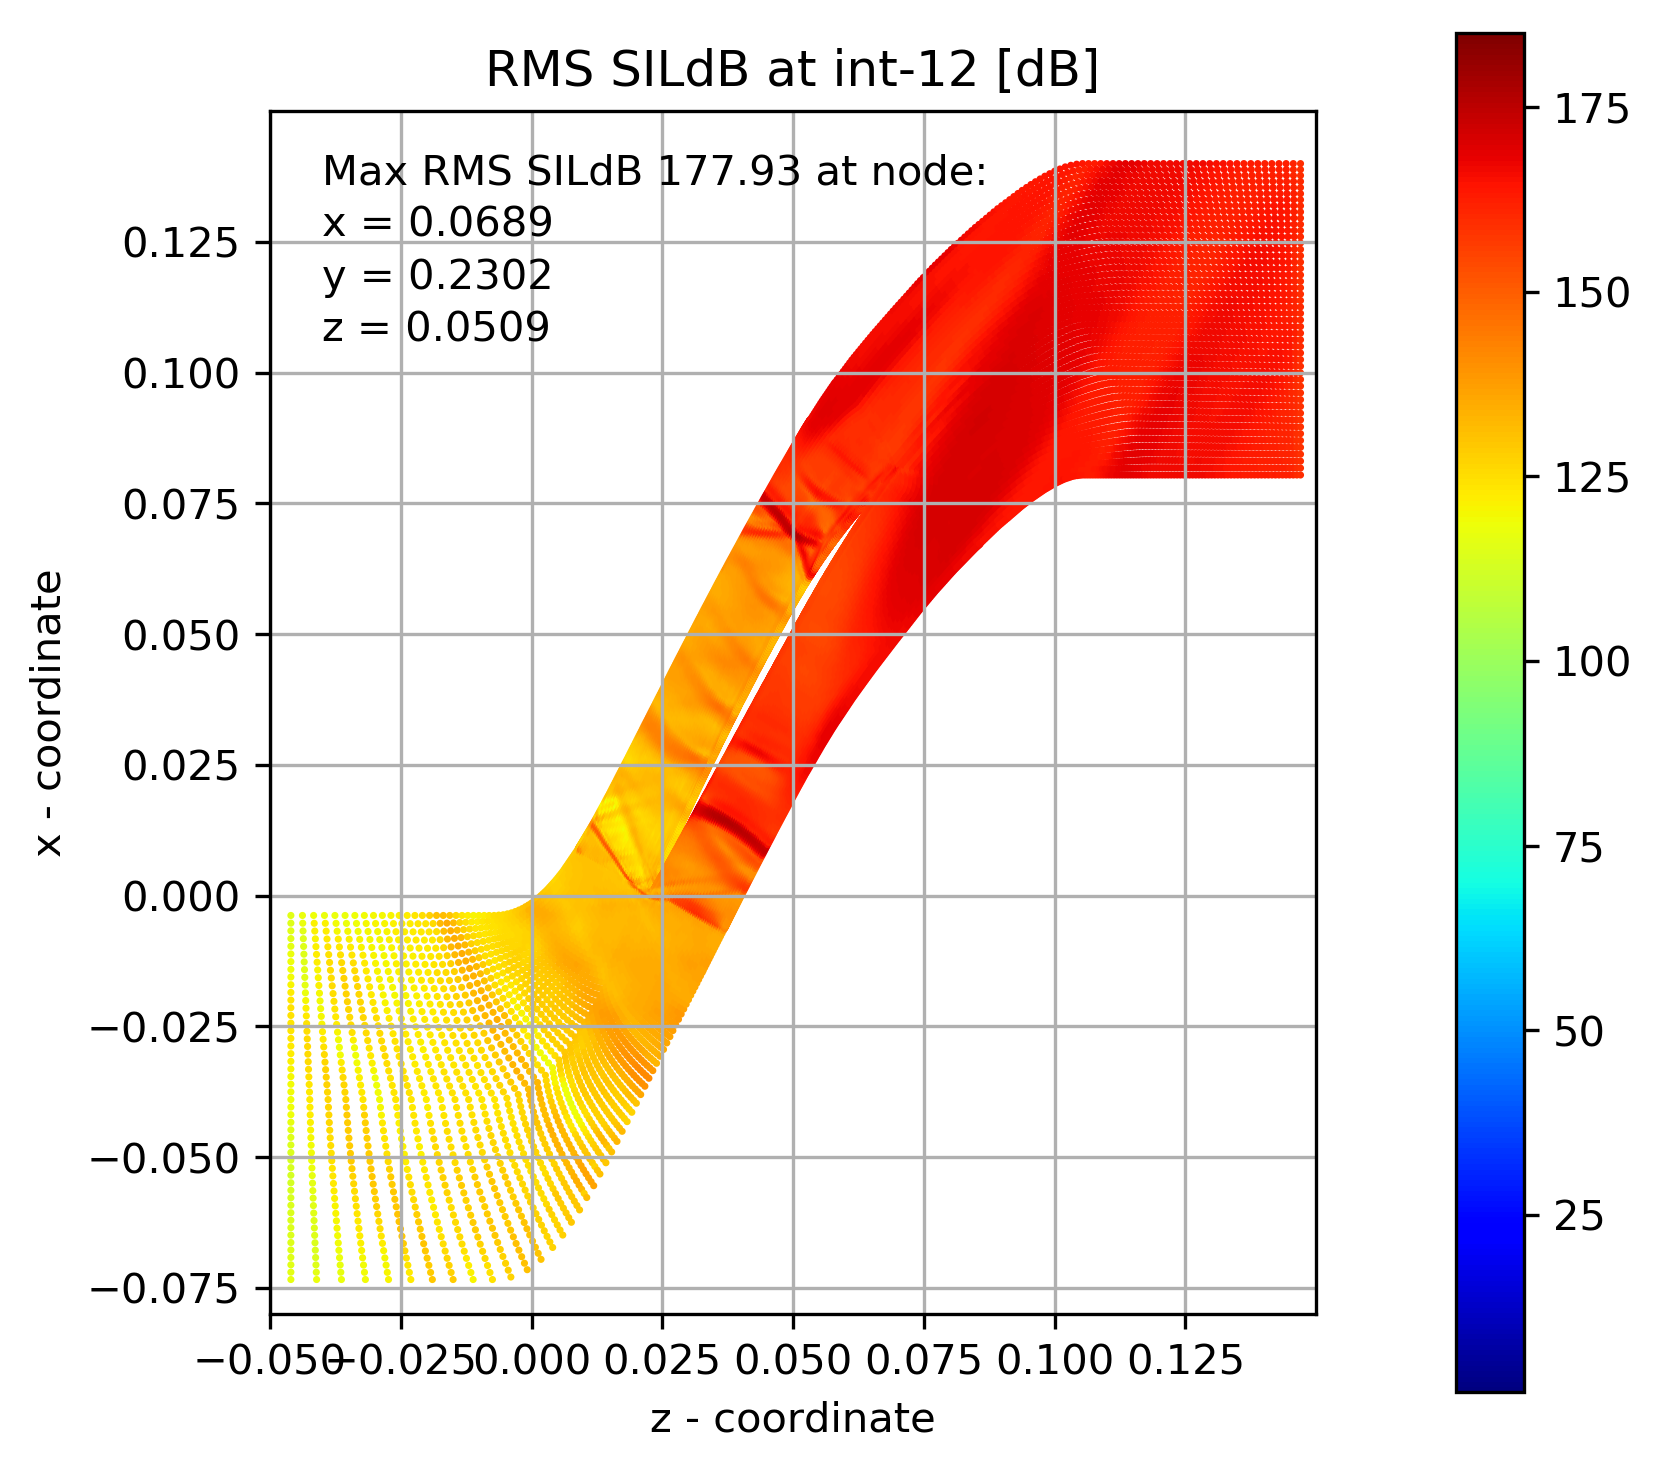
\includegraphics[width=0.75\textwidth]{Figures/int-12-rms-sildb.png} \label{int-12-rms-sildb}
  \caption{RMS Sound intensity decibel level at int-12 mark}
\end{figure}


%int-tip
\begin{figure}[ht]
  \centering
  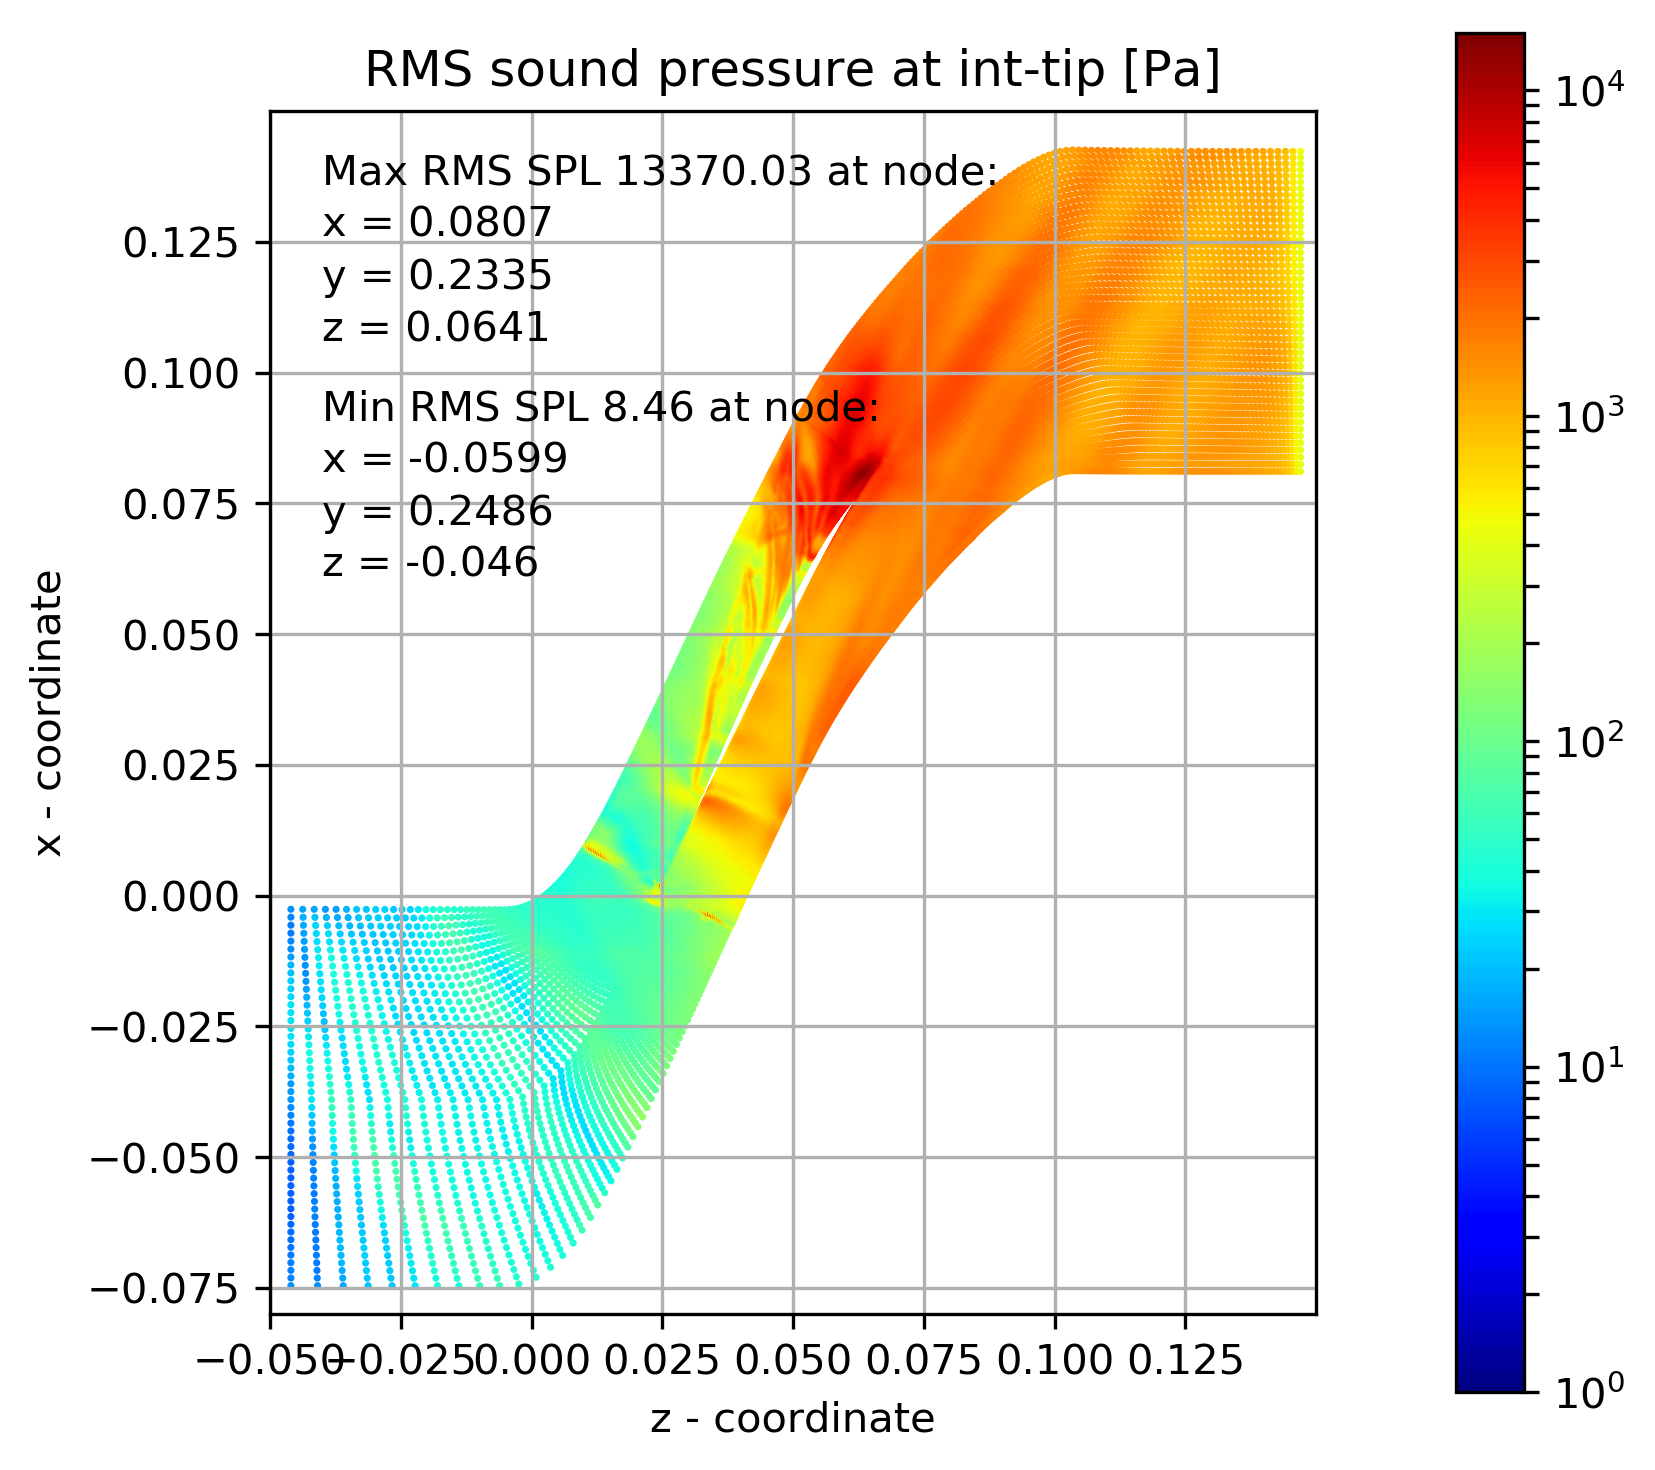
\includegraphics[width=0.75\textwidth]{Figures/int-tip-rms-spl.png} \label{int-tip-rms-spl}
  \caption{RMS Sound pressure at int-tip mark}
  
  \vspace*{\floatsep}% https://tex.stackexchange.com/q/26521/5764

  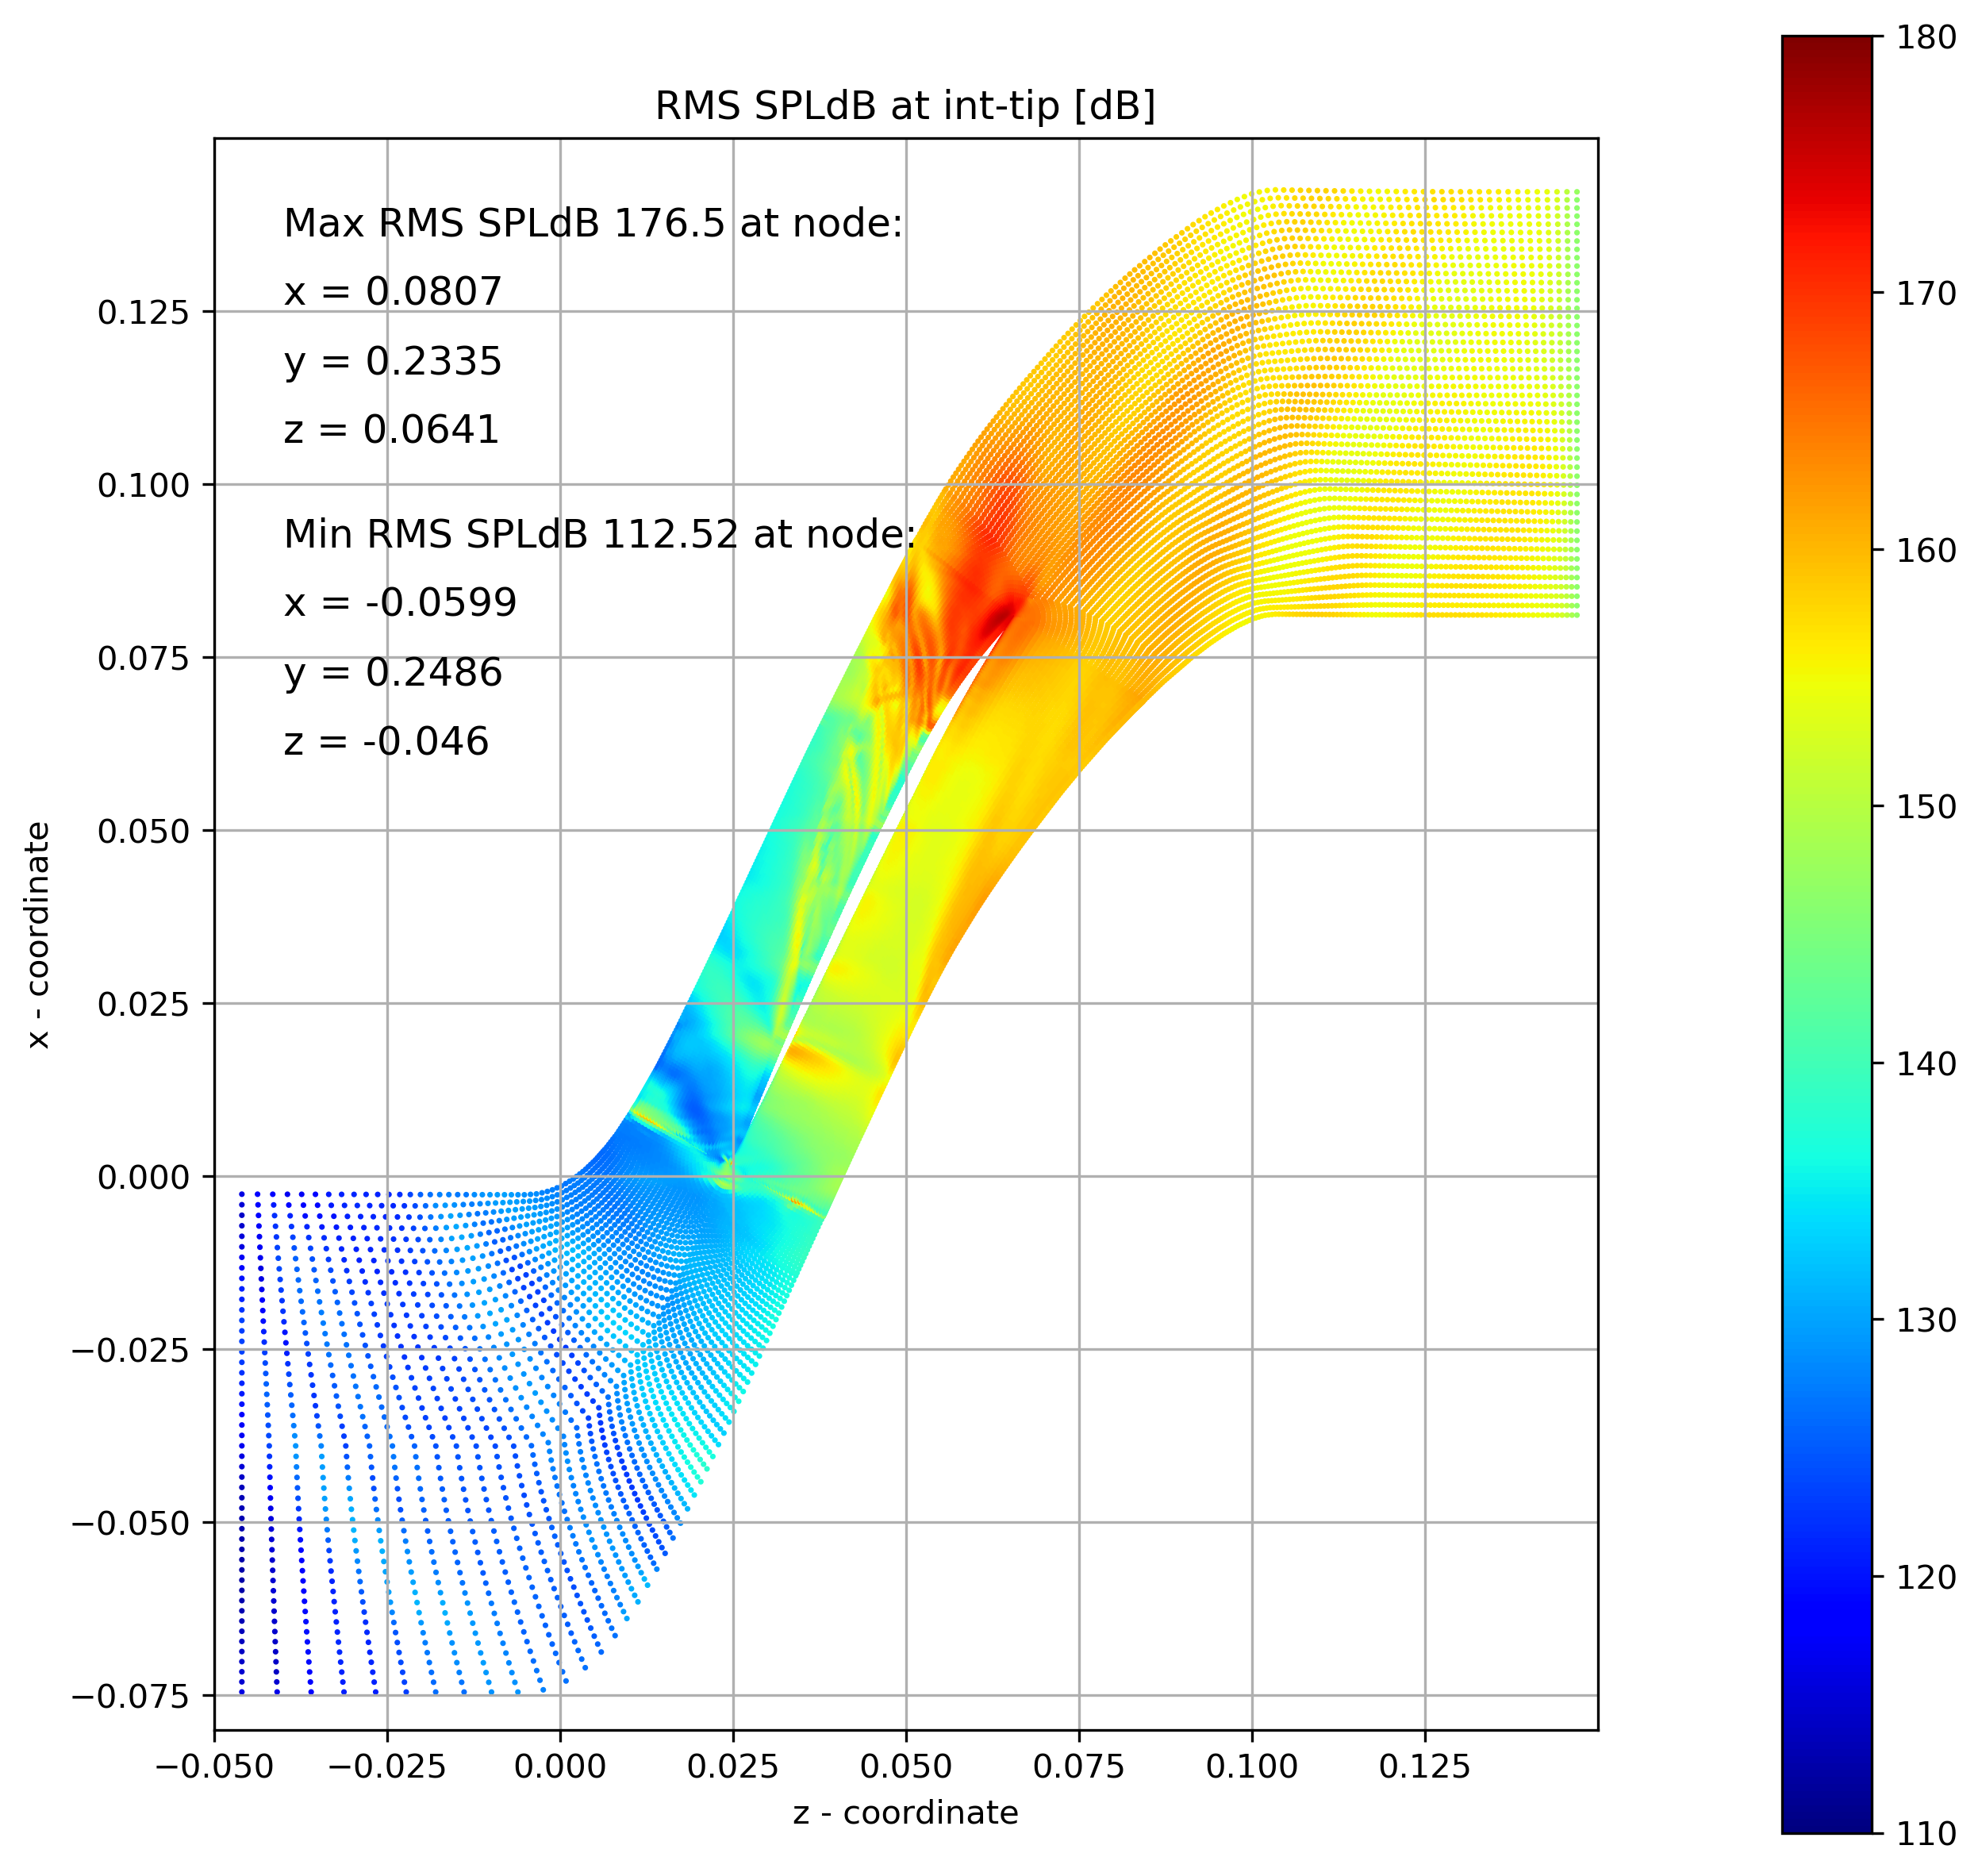
\includegraphics[width=0.75\textwidth]{Figures/int-tip-rms-spldb.png} \label{int-tip-rms-spldb}
  \caption{RMS Sound pressure decibel level at int-tip mark}
\end{figure}
%int-12
\begin{figure}[ht]
  \centering
  \includegraphics[width=0.75\textwidth]{Figures/int-tip-rms-sil.png} \label{int-tip-rms-sil}
  \caption{RMS Sound intensity at int-tip mark}
  
  \vspace*{\floatsep}% https://tex.stackexchange.com/q/26521/5764

  \includegraphics[width=0.75\textwidth]{Figures/int-tip-rms-sildb.png} \label{int-tip-rms-sildb}
  \caption{RMS Sound intensity decibel level at int-tip mark}
\end{figure}